\documentclass[11pt, oneside, openany]{scrbook}
% Layout
\usepackage{geometry}
% Math
\usepackage{mathtools}  % loads amsmath
\usepackage{amssymb}    % loads amsfonts
\usepackage{amsthm}
\usepackage{bbm}
% Tables and figures
\usepackage{array}
\usepackage{booktabs}
\usepackage{multirow}
\usepackage{longtable}
\usepackage{graphicx}
\usepackage{float}
\usepackage{lscape}
% Graphics
\usepackage{xcolor}
% No tikz here: nothing in the body draws any more --- the Bloch sphere is drawn standalone in figures/bloch_sphere.tex.
\usepackage{qcircuit}
% Algorithms
\usepackage{algorithm}
\usepackage{algpseudocode}
% Bibliography
\usepackage{csquotes}
\usepackage[style=numeric,url=false,sortcites=true]{biblatex}
\addbibresource{bibliography.bib}
\DeclareDelimFormat{postnotedelim}{\addcomma\addnbspace} % a postnote stays on its number's line: [20, Thm. 3] never splits
% Hyperlinks and cross-refs (late!)
\usepackage[colorlinks, linkcolor=black, citecolor=black, urlcolor=blue!70!black]{hyperref}
\hypersetup{pdftitle={Symmetry Groups of the Platonic Solid POVMs: Binary Polyhedral Groups as Quantum Circuits}, pdfsubject={Quantum information; binary polyhedral groups; Platonic solid POVMs; classical shadows}, pdfkeywords={binary polyhedral groups; binary icosahedral group; golden gate; exact synthesis; Clifford hierarchy; magic states; SIC-POVM; mutually unbiased bases; informationally complete POVM; classical shadows; robust shadow estimation; dual frame; Naimark dilation; readout twirling; unitary t-designs; Platonic solids}} % indexed by search engines and Scholar; invisible on the page
\usepackage{bookmark}
\usepackage[all]{hypcap} % anchors a float at the top of its box, so a \ref click lands on the figure and not on the caption below it; must follow hyperref.
% Typography (last is fine)
\usepackage{microtype}

% Set depth of Table of Contents
\setcounter{tocdepth}{3} 

% Set depth of section numbering (optional, but recommended if in TOC)
\setcounter{secnumdepth}{3}

\AtEveryBibitem{
  \clearfield{urlday}
  \clearfield{urlmonth}
  \clearfield{urlyear}
  \clearfield{isbn}
  \clearfield{issn}
  % \clearfield{pages}
  \clearfield{url}
  \clearfield{pubstate}
}
\appto{\bibsetup}{\emergencystretch=1em}%

% Set page margins
\geometry{a4paper, margin=1in}

% Define math operators
\DeclareMathOperator{\SU}{SU}
\DeclareMathOperator{\SO}{SO}
\DeclareMathOperator{\U}{U}
\DeclareMathOperator{\PU}{PU}
\DeclareMathOperator{\Tr}{Tr}
\DeclareMathOperator{\Var}{Var}

\newcommand{\C}{\mathbb{C}}
\newcommand{\R}{\mathbb{R}}

% Identity matrix - using \mathbb{1} to distinguish from groups
\newcommand{\Id}{\mathbbm{1}}

% Pauli matrices
\newcommand{\sigmax}{\sigma_x}
\newcommand{\sigmay}{\sigma_y}
\newcommand{\sigmaz}{\sigma_z}
\newcommand{\sigmavec}{\boldsymbol{\sigma}}
\newcommand{\pmat}[1]{\begin{pmatrix} #1 \end{pmatrix}}

% Polyhedral groups - using mathcal to distinguish from identity
\newcommand{\Tgroup}{\mathcal{T}}  % Tetrahedral group
\newcommand{\Ogroup}{\mathcal{O}}  % Octahedral group
\newcommand{\Igroup}{\mathcal{I}}  % Icosahedral group
\newcommand{\Ggroup}{\mathcal{G}}

% Binary polyhedral groups
\newcommand{\TwoT}{2\Tgroup}
\newcommand{\TwoO}{2\Ogroup}
\newcommand{\TwoI}{2\Igroup}
\newcommand{\TwoG}{2\Ggroup}

% Constants
\newcommand{\phig}{\tau} % Golden ratio symbol in Conway/Smith
\newcommand{\invphig}{\sigma} % Inverse golden ratio symbol

% Theorem environments
% NOT scoped to chapter or section. The only numbered statements in the thesis
% are the seven in Appendix~D.1.1, so a flat counter is unambiguous and shortest
% to cite ("by Lemma 2"). Scoping would collide: [chapter] gives "Lemma D.1"
% beside "Appendix D.1", and [section] gives "Theorem D.1.1" beside the
% subsection D.1.1 itself.
\newtheorem{theorem}{Theorem}
\newtheorem{lemma}[theorem]{Lemma}
\newtheorem{corollary}[theorem]{Corollary}
\newtheorem{definition}[theorem]{Definition}
\newtheorem{example}[theorem]{Example}
\newtheorem{remark}[theorem]{Remark}

% Proof sketches (Appendix D.1.1). A proof in every respect but the tombstone: a QED box claims "proved", which a one-line sketch does not. The \renewcommand is local to the environment group, so real proofs keep their box.
\newenvironment{sketch}{\renewcommand{\qedsymbol}{}\begin{proof}[Sketch]}{\end{proof}}

% Helper macros to replace physics package functionality
\newcommand{\ket}[1]{|#1\rangle}
\newcommand{\bra}[1]{\langle#1|}
\newcommand{\braket}[2]{\langle#1|#2\rangle}
\newcommand{\ketbra}[2]{|#1\rangle\langle#2|}
\DeclarePairedDelimiter{\norm}{\lVert}{\rVert}
\DeclarePairedDelimiter{\abs}{\lvert}{\rvert}

\title{Symmetry Groups of the Platonic Solid POVMs}
\subtitle{Binary Polyhedral Groups as Quantum Circuits}
\author{Anton Atanasov Dandarov}
\date{\today}

\begin{document}

\frontmatter

% ===== JKU cover sheet (replaces \maketitle) ==================================
\begin{titlepage}
\sffamily
\noindent
\begin{minipage}[t]{0.58\textwidth}\vspace{0pt}%
{\huge\bfseries Symmetry Groups of the\\Platonic Solid POVMs\par}
\vspace{6mm}
{\large Binary Polyhedral Groups as Quantum Circuits\par}
\end{minipage}\hfill
\begin{minipage}[t]{0.34\textwidth}\vspace{0pt}\raggedright\small

\includegraphics[width=\linewidth]{figures/jku_en_black.pdf}\\[8mm]
\textbf{Author}\\[1mm]
To Be Finalized\\[5mm]% Anton Atanasov Dandarov\\[5mm]
\textbf{Submission}\\[1mm]
Institute for Integrated Circuits and Quantum Computing\\[5mm]
\textbf{Thesis Supervisor}\\[1mm]
To Be Finalized\\[5mm]% Univ.-Prof.\ Dr.\ Richard Kueng\\[5mm]
\textbf{Assistant Thesis Supervisor}\\[1mm]
To Be Finalized\\[5mm]% Jadwiga Wilkens, MSc\\[5mm]
September 2026
\end{minipage}
\vfill
\noindent
\begin{minipage}[b]{0.58\textwidth}\small
Bachelor's Thesis\\
to confer the academic degree of\\
Bachelor of Science\\
in the Bachelor's Program\\
Artificial Intelligence
\end{minipage}\hfill
\begin{minipage}[b]{0.34\textwidth}\raggedright\small
JOHANNES KEPLER\\
UNIVERSITY LINZ\\
Altenberger Str.\ 69\\
4040 Linz, Austria\\
jku.at
\end{minipage}
\end{titlepage}

% ===== Sworn declaration (JKU bachelor wording, verbatim) =====================
\thispagestyle{empty}

\begin{center}\bfseries\Large Sworn Declaration\end{center}

\bigskip

\noindent I hereby declare under oath that the submitted Bachelor Thesis has been written solely by me without any third-party assistance, information other than provided sources or aids have not been used and those used have been fully documented. Sources for literal, paraphrased and cited quotes have been accurately credited. The submitted document here present is identical to the electronically submitted text document.

\bigskip

\noindent\textbf{Aids used.} Anthropic's Claude was used throughout as a research and engineering aid.

\clearpage

\begin{center}\bfseries\Large Abstract\end{center}


\bigskip

We study the symmetry groups of the Platonic solid POVMs: the binary polyhedral groups $\TwoT$, $\TwoO$, and $\TwoI$, exact unitary $2$-, $3$-, and $5$-designs. A unified treatment, bringing together mathematical construction, quantum circuits, and cost, is missing. We provide it, in the single-qubit setting, via two complementary constructions and a compilation, implemented with symbolic computation. The result is an atlas of all 192 group elements, fully reproducible from accompanying code, its gate sequences, none deeper than four, doubling as POVM rotation circuits. Once anchored to the Pauli group, $\TwoT$ and $\TwoO$ are entirely Clifford, while the binary icosahedral group $\TwoI$ requires at most one non-Clifford gate per element---the golden gate $\Phi$. As a double-coset decomposition, $\TwoI = \TwoT \sqcup \TwoT\,\Phi\,\TwoT$. We prove that only the octahedral POVM admits exact implementation over our gate sets (Clifford${}+T$ among them), and never deterministically; in our orientation, the other four point at magic states. We consider the POVMs in classical shadow estimation, where an inexact implementation is paid for in estimator variance; scalability keeps us to local shadows, a per-qubit factorized regime. We compare two randomized implementations: both support robust shadow estimation, but calibrate different scalars; calibration must match protocol. Every Platonic solid POVM has a Naimark dilation circuit, though never an exact one, and a prepended draw from $\TwoT$, the least group that suffices, twirls measurement-side noise to exactly depolarizing (and makes approximation cost variance, never bias). Only the antipodal solids decompose into projective measurements, which excludes the tetrahedral SIC. There, one drawn rotation must both realize the POVM and twirl the noise: among groups, granted by $\TwoT$ for all but the dodecahedron, which requires $\TwoI$.

\clearpage

\microtypesetup{protrusion=false} % disables protrusion locally in the document
\tableofcontents % prints Table of Contents
\microtypesetup{protrusion=true} % enables protrusion

\mainmatter

\chapter{Introduction}

Quantum measurements rich in symmetry are in vogue---symmetry pays, especially so in dimensionality-cursed settings. A pivotal abstraction is that of the $t$-design, and we will see spherical, complex projective, and unitary $t$-designs all come into play. In particular, rank-one tight informationally complete POVMs are exactly (weighted) complex projective $2$-designs and are optimal for linear state tomography~\cite{scott2006tightinformationallycomplete}. In the single-qubit case, inscribing a Platonic solid in the Bloch sphere---its vertices the outcomes---yields one such optimal measurement, inheriting the solid's symmetry: the tetrahedron is \textit{the} SIC-POVM, the octahedron the complete set of MUBs, and the icosahedron a tight (fewest-points) projective $5$-design~\cite{lyubich2007tightprojectivedesigns,nasmith2023tight}.

Behind each such measurement stands a group. The rotations carrying a Platonic solid to itself form its symmetry group (dual solids share theirs, so the five solids yield three groups), and these lift, through the $\SU(2)\to\SO(3)$ double cover, to the \textit{binary polyhedral groups} $\TwoT$, $\TwoO$, and $\TwoI$---the three exceptional finite subgroups of $\SU(2)$, and the unitaries that permute the outcomes of the corresponding POVM. These same groups have garnered attention in fault-tolerant quantum computation: the binary icosahedral group $\TwoI$, paired with a single $T$-like gate, gives a remarkably efficient single-qubit universal gate set~\cite{parzanchevski2018supergoldengatespu2,blackman2022fastnavigationicosahedral}, even as it harbors an exotic gate $\Phi$ that lies outside the Clifford hierarchy~\cite{kubischta2023familyquantumcodes}. The symmetry group behind the measurement, then, is also behind a gate set---making the group itself a natural object of study.

The necessary pieces exist, yet in separate literatures. How to construct the groups is found in mathematical expositions~\cite{conway2009quaternionsoctonionstheir,coxeter1973regularpolytopes,vanhoboken2002platonicsolidsbinary}, written for algebra and geometry rather than quantum use. Circuits for the Platonic solid POVMs \textit{are} given---by \textcite{decker2004quantumcircuitssinglequbit}---but that work predates the modern design, shadow~\cite{huang2020predictingmanyproperties}, and $\TwoI$ developments and does the POVM circuit \textit{only}. Discussion of gate cost is in the golden-gate~\cite{parzanchevski2018supergoldengatespu2,blackman2022fastnavigationicosahedral}, stabilizer~\cite{bravyi2019simulationquantumcircuits}, and hardware~\cite{barends2014rollingquantumdice} literatures, but without treating measurement.

On the measurement side, close to a unified account is the classification of highly symmetric qubit POVMs by \textcite{slomczynski2015highlysymmetricpovms}, which organizes them by symmetry but stops at their informational power; \textcite{nguyen2020symmetriesmeasurementsquantum} build symmetric measurement assemblages \textit{from} a group and its unitary representation, never examining circuits. On the fault-tolerance side, a rare bridge is the twisted unitary $t$-group construction of \textcite{kubischta2024quantumcodestwisted}, which links designs to codes, but not measurements. No single account puts the pieces together. Once the group behind a Platonic solid POVM must run as gates, what does its symmetry exact?

This thesis provides that account: it constructs the three binary polyhedral groups, circuit-implements them, and weighs what they cost. Its central artifact is a unified, cost-aware atlas of all three groups, backed by symbolic computation, whose gate sequences double as rotation circuits for the POVMs. We give the complete single-qubit picture. We find $\TwoI$, though exotic, to be \textit{almost Clifford}: every element realizable with at most a single $\Phi$ gate. Over every gate set here---$\TwoT$, Clifford, Clifford${}+T$, $\TwoI$, Clifford${}+\Phi$---only the octahedral POVM admits an exact implementation, and never deterministically. A randomized implementation is here one of two protocols: prepending a drawn rotation to a dilation circuit, or the drawn rotation itself realizing the POVM projectively.
% NOTE: This is the contributions paragraph.

Several threads run throughout this thesis. The first is geometry. The solids enter as measurements, inscribed in the Bloch sphere, with vertices as outcomes. One dimension up, the groups themselves form vertex sets of highly symmetric 4D configurations ($\TwoT$ the 24-cell, $\TwoO$ its union with its dual, $\TwoI$ the 600-cell), a correspondence we exploit for one of our constructions. Moreover, the 24-cell completes to a 600-cell in two ways, via even or odd coordinate permutations. This means that $\SU(2)$ holds two copies of $\TwoI$ over the same $\TwoT$; our atlas commits to one, and the choice descends to the Bloch sphere, splitting the icosahedral measurements into two families, no single group copy serving both.

The second thread is gate sequences. Once anchored to a fixed copy of the Pauli group, the groups are generated by \textit{named} gates (the Paulis among them), and group questions become circuit questions: which elements are Clifford, how deep a sequence must run, how much exotic (non-Clifford) resource it requires. In fact, the anchored $\TwoO$ \textit{is} the single-qubit Clifford group $\mathcal{C}_1$, and $\TwoT$ sits inside it. The atlas of Appendix~\ref{app:atlas} answers element by element, and we then show that the single-$\Phi$ ceiling for $\TwoI$ is forced---a double-coset decomposition, $\TwoI = \TwoT \sqcup \TwoT\,\Phi\,\TwoT$. We adopt the fault-tolerant cost model, with Clifford gates cheap and non-Clifford ones dear.

The third thread is the measurements themselves. We define the POVMs as \textit{transitive covariant}: the group carries any effect to any other (so all effects have equal trace). They exhibit high design strengths, which depend only on the group, not the solid. It is in robust shadow estimation that we finally consider them in use. There, the two randomized implementations render measurement-side noise exactly depolarizing, each with its own gate overhead, while an unrandomized one saves the gates and pays with a calibration blind spot.

Binding the threads together is algebra. We use a small toolkit repeatedly: equivariance becomes covariance, orbit--stabilizer does decisive counting, and Schur's lemma fixes the form of the effects, before returning to settle a noise question at the end. Two cases recur as exceptions. The icosahedral group is the largest of the three, bringing with it the exotic gate $\Phi$, the golden ratio in its matrix entries. The tetrahedron is the one solid without antipodal vertices, so the one measurement no mixture of projective measurements can realize; its POVM (the SIC) is indecomposable~\cite{dariano2005classicalrandomnessquantum}, in fact a mixture of no other measurements at all. 

The preliminaries of Chapter~\ref{cha:theoreticalbackground} are standard; the fluent reader may start at Section~\ref{sec:platonic-solids}. Much of this thesis is in its appendices, deliberately. The central artifact is one of them: Appendix~\ref{app:atlas} is the atlas, all three groups element by element, with the POVM coordinates it acts on in Appendix~\ref{app:povm-atlas}; both are data. Appendix~\ref{app:decker} carries the five POVM circuits and the proofs of the exactness claim above; Appendix~\ref{app:shadows} derives the estimator channel and the gate overhead of each randomized implementation; Appendix~\ref{app:synthesis} proves the single-$\Phi$ ceiling forced and prices $\Phi$ itself; all three are argument. Appendix~\ref{app:rotations} is reference, cited in passing. The code is in an accompanying repository at \url{https://github.com/ArachnidaDuality/platonic-povm-groups}; reproduction is one \texttt{uv run} command.

Figure~\ref{fig:tetrahedron-recipe}, on the next page, works the tetrahedron in six steps: from four Bloch vectors to four effects, through the circuit that performs them, to the twelve rotations that permute their outcomes and, drawn uniformly, twirl the noise; a foot strip gives a brief on all five solids, which each also get a similar figure in Appendix~\ref{app:decker}. Each step names where the thesis derives it, so the one case worked up front is also an itinerary.


% Figure 1.1 --- the complete recipe, worked on the tetrahedron.
\begin{figure}[p]
  % Figure 1.1 --- "The tetrahedral POVM, end to end".  The layout only.
%
% LAYOUT AS INSTRUCTION: the six numbered steps are the band headers, so the
% page's skeleton and its instructions are one object.  Under each header sits
% the thing that discharges it; at each header's right margin sits the thesis
% pointer that derives it, so the right edge reads as a table of contents for
% the seventeen pages that follow.  The banner carries one too, and it is the
% only one that points at a page rather than a derivation: the five Appendix D
% cards run these same steps on the other four solids, and each of them points
% back here from its own title line.  Every pointer is a live \ref --- this file
% is \input into bsc-thesis.tex rather than compiled as one standalone PDF
% exactly so that a moved appendix cannot rot a baked-in "Table E.1".
%
% The six numerals must read 1..6 straight down the left edge: the banner
% promises "the order one uses them", so step 4 (predict/invert) sits at the
% FOOT of band B, after the bits have been read, not at the foot of band A.
%
% Everything numeric comes from code/data/recipe_tet_data.tex (beside the
% other fragments the thesis \input's from there), which
% code/_build_recipe_figure.py writes after twelve assertions against the npz
% data and Tables A.1, 5.2, D.1, D.3 and D.4.  The twelfth reads THIS file and
% checks the permutations, pair numbers, angles and identities quoted in the
% prose below against the computed group -- so the sentences may be rewritten
% freely, but the facts in them cannot drift.  Only the prose and the step
% heads are hand-written here; the caption lives in bsc-thesis.tex.
%
% ASSEMBLY RULES (each one bought with a measurement; do not "tidy" them):
%   * rows are stacked in one \vbox and separated by \vskip<n>pt\nointerlineskip.
%     Without \nointerlineskip LaTeX adds ~13.6pt of baseline glue PER ROW and
%     the page runs ~150pt over its budget.
%   * a two-column row is one \hbox to \hsize{<left>\hfil<right>} whose columns
%     are \vtop's opening with \hbox{}\nointerlineskip, which is what top-aligns
%     them (a \vtop otherwise aligns on its first line's baseline).
%   * every prose block is \PBOX: \sloppy plus \emergencystretch, or the
%     unbreakable math atoms throw overfull boxes into the neighbouring column.
%   * graphics are centred with \CTR (\hss ... \hss) and not \centerline,
%     which would report the overhang as overfull.  The circuit is the one
%     exception: its 307.5bp page carries all 13.7bp of xy-pic's slack on the
%     RIGHT (measured ink 0.648..293.816bp), so centring its box hangs the
%     \lstick ket bar ~1.4pt into the left margin.  It is set flush left
%     instead, which puts the ket bar 0.65pt inside the column, on the same
%     vertical as the step numerals and the four band rules.
%   * exactly four band rules.  No other rules, no boxes, no tints, no colour.
%   * every step head must fit on ONE line; an overfull head collides with its
%     own pointer.
%
% WORDING RULES (each is a constraint on the prose, not a suggestion):
%   * the rotation table's last column is the READING, g^{-1}: "I prepended
%     your word and read 1234 -- what did I measure?"  Head 5 is what defines
%     it ("outcomes 1234 then read as its row"), rider 4 gives the worked case,
%     and the frames read site by site are the same rows.  The generator
%     emits g^{-1} and checks all twelve off the rebuilt circuit; the price is
%     that readings compose in reverse operator order, which the page never
%     prints (pair 10's example is order-blind).
%   * bold by the claim, not the noun: rotation claims plain ("$F$ turns the
%     labelled solid", "with $F$, outcomes ... read as", "$Z$ then $X$ ... is
%     pair 10's half-turn"), SU(2) claims bold ($\mathbf F^3=-\Id$,
%     $\mathbf{XZ}=-\mathbf{ZX}$, the words in the table).  Rider 3 carries
%     both fonts in one sentence on purpose: that IS its point.
%   * no italic run-in heads (the thesis has none); riders open as plain
%     sentences.
%   * the two protocol names: twirled-native stays, defined in place and
%     hyperlinked to its section; randomized-projective does not appear --
%     the strip's head is "coin over axes" (hyperlinked to the coin words,
%     Table D.1), so band B's "the coin below" lands on a column that says
%     coin, and the printed octahedral set on the row the link opens.
%   * no cold "Decker's" in the body: the caption carries the name and the
%     cite; the body says "the published circuit" and "this one included".
%
% All macros below are \def and therefore local to the figure environment.
\parindent=0pt \parskip=0pt
% Auto-generated by code/_build_recipe_figure.py -- DO NOT EDIT.
% The four data blocks of Figure 1.1 (paper/figures/recipe_tet_body.tex
% \input's this as ../code/data/recipe_tet_data and calls them).  Every number is derived from code/data/*.npz and checked back
% against Tables A.1, 5.2, D.1, D.3 and D.4 before this file is written; see
% the builder's docstring for the twelve assertions.
% Requires: booktabs, mathtools, hyperref, and the thesis macros \Id, \pmat,
% \bra, \ket, \TwoT, \TwoO, \TwoI.
% Regenerate with `cd code && uv run _build_recipe_figure.py`.

\newcommand{\RecipeMasterTable}{{\small
\setlength{\tabcolsep}{4pt}\renewcommand{\arraystretch}{0.90}%
\begin{tabular}{@{}c l c c r@{}}
\toprule
$k$ & $\hat n_k\ (\times\tfrac{1}{\sqrt3})$ & $E_k\ (\times\tfrac{\sqrt3}{12})$ & bits & $\bra{0}E_k\ket{0}$ \\
\midrule
1 & $(+1,+1,+1)$ & $\pmat{\sqrt3+1 & 1-i \\ 1+i & \sqrt3-1}$ & $00$ & $0.3943$ \\
2 & $(-1,-1,+1)$ & $\pmat{\sqrt3+1 & -1+i \\ -1-i & \sqrt3-1}$ & $01$ & $0.3943$ \\
3 & $(-1,+1,-1)$ & $\pmat{\sqrt3-1 & -1-i \\ -1+i & \sqrt3+1}$ & $10$ & $0.1057$ \\
4 & $(+1,-1,-1)$ & $\pmat{\sqrt3-1 & 1+i \\ 1-i & \sqrt3+1}$ & $11$ & $0.1057$ \\
\bottomrule
\end{tabular}}}

\newcommand{\RecipeCircuitParams}{%
$U_A=\sqrt2\bigl(\begin{smallmatrix}\alpha & \beta\\ \beta & -\alpha\end{smallmatrix}\bigr)$\par
$T^\dagger=\mathrm{diag}(1,e^{-i\pi/4})$\par
\vskip1pt $\alpha=\sqrt{(3{+}\sqrt3)/12}=0.6280$\par
$\beta=\sqrt{(3{-}\sqrt3)/12}=0.3251$}

\newcommand{\RecipeRotationTable}{{\small
\setlength{\tabcolsep}{3pt}\renewcommand{\arraystretch}{0.88}%
\begin{tabular}{@{}r l l c c@{}}
\toprule
pair & $a$-word & $b$-word & axis & $1234\mapsto$ \\
\midrule
1 & $\Id$ & $\mathbf{X}\mathbf{X}$ & --- & 1234 \\
2 & $\mathbf{F}$ & $\mathbf{F}^{\dagger}\mathbf{F}^{\dagger}$ & $\hat n_1$ & 1342 \\
3 & $\mathbf{F}^{\dagger}$ & $\mathbf{F}\mathbf{F}$ & $-\hat n_1$ & 1423 \\
4 & $\mathbf{X}$ & $\mathbf{X}^{\dagger}$ & $\hat x$ & 4321 \\
5 & $\mathbf{Z}$ & $\mathbf{Z}^{\dagger}$ & $\hat z$ & 2143 \\
6 & $\mathbf{F}\mathbf{X}$ & $\mathbf{F}\mathbf{X}^{\dagger}$ & $\hat n_2$ & 4213 \\
7 & $\mathbf{F}^{\dagger}\mathbf{Z}$ & $\mathbf{F}^{\dagger}\mathbf{Z}^{\dagger}$ & $-\hat n_4$ & 2314 \\
8 & $\mathbf{X}\mathbf{F}$ & $\mathbf{X}^{\dagger}\mathbf{F}$ & $\hat n_3$ & 2431 \\
9 & $\mathbf{X}\mathbf{F}^{\dagger}$ & $\mathbf{X}^{\dagger}\mathbf{F}^{\dagger}$ & $-\hat n_2$ & 3241 \\
10 & $\mathbf{X}\mathbf{Z}$ & $\mathbf{X}\mathbf{Z}^{\dagger}$ & $\hat y$ & 3412 \\
11 & $\mathbf{Z}\mathbf{F}$ & $\mathbf{Z}^{\dagger}\mathbf{F}$ & $\hat n_4$ & 3124 \\
12 & $\mathbf{Z}\mathbf{F}^{\dagger}$ & $\mathbf{Z}^{\dagger}\mathbf{F}^{\dagger}$ & $-\hat n_3$ & 4132 \\
\bottomrule
\end{tabular}}}

\newcommand{\RecipeSeriesStrip}{{\footnotesize
\setlength{\tabcolsep}{4pt}\renewcommand{\arraystretch}{0.88}%
\begin{tabular}{@{}l c c c c l l l@{}}
\toprule
The same six steps run & $V$ & group & anc. & dead & reorientation exact? & relabelling & \hyperref[tab:decker-vs-coin]{coin over axes} \\
\midrule
\textbf{Tetrahedron} & \textbf{4} & $\TwoT$ & 1 & 0 & $T^\dagger$, over Clifford${}+T$ & identity & none: no antipodes \\
Octahedron & 6 & $\TwoO$ & 2 & 2 & no thesis gate set & permuted & 3 axes --- \textbf{exact} \\
Cube & 8 & $\TwoO$ & 2 & 0 & $T^\dagger$, over Clifford${}+T$ & permuted & 4 axes \\
Icosahedron & 12 & $\TwoI$ & 3 & 4 & no thesis gate set & permuted & 6 axes, no $\Phi$ \\
Dodecahedron & 20 & $\TwoI$ & 4 & 12 & no thesis gate set & permuted & 10 axes, 4 with one $\Phi$ \\
\bottomrule
\end{tabular}}}

\long\def\NIS#1{\vskip #1\nointerlineskip}
\long\def\CTR#1#2{\hbox to #1{\hss #2\hss}}
\long\def\PBOX#1#2{\vtop{\hsize=#1\parindent0pt\sloppy\emergencystretch=1.5em\footnotesize #2}}
\long\def\COL#1#2{\vtop{\hsize=#1\parindent0pt\hbox{}\nointerlineskip #2}}
\long\def\FULLHEAD#1#2#3{\hbox to \hsize{\small\textbf{#1}\,#2\hfil{\footnotesize #3}}}
\def\BANDRULE{\vskip3pt\hrule height0.5pt\vskip3pt\nointerlineskip}
%
\vbox{\hsize\textwidth\parindent0pt
%
% --- banner ---------------------------------------------------------------
\hbox to \hsize{\large\bfseries The tetrahedral POVM, end to end\hfil{\normalfont\footnotesize All five solids in Appendix~\ref{app:decker}}}%
\NIS{2pt}%
\PBOX{\hsize}{Six steps, in the order one uses them; each names where this
thesis derives it. Operator order: $\mathbf{FX}$ applies $\mathbf X$ first.}%
\BANDRULE
%
% --- band A: step 1 --------------------------------------------------------
\FULLHEAD{1}{Take the four Bloch vectors; make each one an effect,
  $E_k=\tfrac{1}{V}(\Id+\hat n_k\cdot\sigmavec)$.}%
  {Table~\ref{tab:povm-atlas} $\cdot$ Equation~\eqref{eq:povmform}}%
\NIS{4pt}%
\hbox to \hsize{%
  \COL{166pt}{\CTR{166pt}{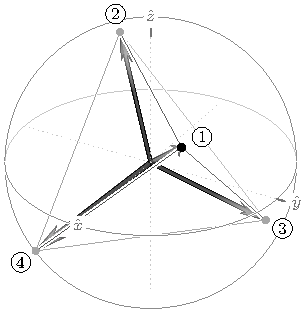
\includegraphics{figures/recipe_tet_sphere.pdf}}}%
  \hfil
  \COL{276pt}{\CTR{276pt}{\RecipeMasterTable}%
    \NIS{4pt}%
    \PBOX{276pt}{$V=4$;
      $\sum_k E_k=\Id$; $\Tr E_k=\tfrac12$; each rank one;
      $|\braket{\psi_j}{\psi_k}|^2=\tfrac13$ for $j\neq k$: the SIC condition,
      at the Welch bound.}}%
}%
\BANDRULE
%
% --- band B: steps 2, 3 and 4 ----------------------------------------------
% Head 2 names the dashed box and says it is off: everything printed in this
% band---the four probabilities, the bits, the outcome key---is the circuit
% run WITHOUT the U_g prefix, and the alpha^2 claim below is only true so.
% Head 3 gives the bit order, because a reader who takes the bits
% data-wire-first swaps vertices 2 and 3 on every shot; ancilla-first (top
% wire) is Table D.4's own convention and what assertion 9's rebuild returns.
\FULLHEAD{2}{Run this circuit, step~5's dashed box omitted; measure both
  wires.}%
  {Figure~\ref{fig:tet_povm_circuit} $\cdot$ Appendix~\ref{app:decker}}%
\NIS{2pt}%
\FULLHEAD{3}{Read the two bits, top wire first, as a vertex.}%
  {Table~\ref{tab:decker-labels}}%
\NIS{4pt}%
\hbox to \hsize{%
  \COL{306pt}{\hbox to 306pt{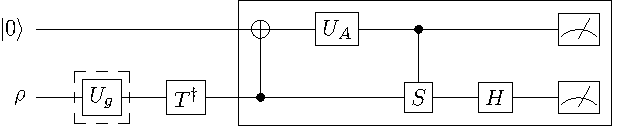
\includegraphics{figures/recipe_tet_circuit.pdf}\hss}}%
  \hfil
  \COL{136pt}{\PBOX{136pt}{\RecipeCircuitParams}}%
}%
\NIS{3pt}%
% The opening clause is the one sentence on the page that says what a
% reorientation IS (the strip's "reorientation exact?" column is unparseable
% without it); the generator checks it off the rebuilt circuit (check 9: the
% box without T-dagger measures our effects turned 45 degrees about z).
% The exactness sentence is the thesis's own (Sections 4.2.2 and 5.1) and each part
% of it is load-bearing: the italic on \textit{deterministic}, without which
% the two clauses read as a flat contradiction; the parenthetical "any
% dilation, this one included", which is what says the circuit printed just
% above is not exact; and "admits an exact implementation", which must not be
% reduced to a pronoun.  Four lines.  What paid for the opening clause is
% "each also the top-left entry of its own E_k" --- the master table's last
% head now reads <0|E_k|0>, which says the same thing beside the matrices.
\PBOX{\hsize}{$T^\dagger$ reorients the published circuit, the solid box, to
  our pose. On $\rho=\ketbra{0}{0}$ the data wire is untouched until the
  final $H$, so the four probabilities are $\alpha^2,\alpha^2,\beta^2,\beta^2$:
  the $\bra{0}E_k\ket{0}$ column above---but no \textit{deterministic}
  protocol over any gate set of this thesis---any dilation, this one
  included---implements any Platonic solid POVM exactly
  (Theorem~\ref{thm:main}); only the octahedral POVM admits an exact
  implementation, exhibited by the coin below, $\{\Id, \mathbf F, \mathbf F^\dagger\}$.}%
\NIS{4pt}%
\FULLHEAD{4}{Predict $p(k)=\Tr[E_k\rho]=\tfrac14(1+\hat n_k\cdot r)$; or
  invert, $r=3\sum_k p(k)\hat n_k$.}%
  {Section~\ref{sec:platonic-solid-povms} $\cdot$ Appendix~\ref{sec:shadows:setup}}%
\BANDRULE
%
% --- band C: steps 5 and 6 -------------------------------------------------
% Head 5 defines the rotation table's last column: the reading, g^{-1}.
\FULLHEAD{5}{Rotate it: prepend one atlas word; outcomes $1234$ then read as
  its row.}%
  {Table~\ref{tab:binary-tetrahedral-group-2t} $\cdot$ Section~\ref{subsec:rotated-povms}}%
\NIS{2pt}%
\FULLHEAD{6}{Twirl: draw that word uniformly.}%
  {Section~\ref{subsec:randomized-implementations} $\cdot$ Appendix~\ref{sec:shadows:channels}}%
\NIS{4pt}%
\hbox to \hsize{%
  \COL{156pt}{\RecipeRotationTable}%
  \hfil
  \COL{290pt}{\CTR{290pt}{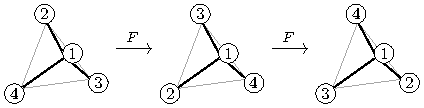
\includegraphics{figures/recipe_tet_frames.pdf}}%
    \NIS{3pt}%
    \PBOX{290pt}{$F$ turns the labelled solid $120^\circ$ about
      vertex~1's axis; twice is pair~3, a third brings it home---but
      $\mathbf F^3=-\Id$. Pairs 4, 5, 10 turn $180^\circ$.\par\vskip3pt
      Twelve rotations, twenty-four unitaries: each pair is one rotation and
      two atlas words $\pm U$---pair~2 is $\mathbf F$ and
      $\mathbf F^\dagger\mathbf F^\dagger=-\mathbf F$, both
      $1234\mapsto1342$.\par\vskip3pt
      Two permutations make one: $Z$ then $X$, or $X$ then $Z$, is pair~10's
      half-turn about $\hat y$---but $\mathbf{XZ}=-\mathbf{ZX}$; the order
      shows up only as the sign.\par\vskip3pt
      Prepending $U_g$ rotates the effects by $g^{-1}$: with $F$, outcomes
      $1,2,3,4$ read as vertices $1,3,4,2$. Drawn afresh each shot and
      relabelled, that is
      \hyperref[subsec:randomized-implementations]{\textit{twirled-native}},
      and measurement-side noise then averages to depolarizing.}}%
}%
\BANDRULE
%
% --- band D: the series strip ----------------------------------------------
\CTR{\hsize}{\RecipeSeriesStrip}%
}%

  \caption{\textbf{The tetrahedral POVM, end to end.} Every object is assembled from later chapters and checkable against them---the vectors from Table~\ref{tab:povm-atlas}, in the pose of Figure~\ref{fig:platonic-solid-povms}, the effects from Equation~\eqref{eq:povmform}, the circuit from Figure~\ref{fig:tet_povm_circuit} after \textcite{decker2004quantumcircuitssinglequbit}, the twelve rotations from Table~\ref{tab:binary-tetrahedral-group-2t}.}
  \label{fig:tetrahedron-recipe}
\end{figure}
\clearpage

\chapter{Theoretical Background} \label{cha:theoreticalbackground}

This chapter collects what the rest of the thesis uses, and no more. Sections~\ref{sec:quantuminfobasics} and~\ref{sec:measurement} are standard quantum information; the thesis's own objects begin at Section~\ref{sec:platonic-solids}, the quaternion convention $U_q$ sits in Section~\ref{subsec:su2-h1}, and the algebra is introduced where it is used.

\section{Quantum Information and Computing Basics} \label{sec:quantuminfobasics}

Quantum information processing is a paradigm of its own, and not merely a flavor of classical computing; this section fixes the notation, and the introductory texts carry the rest~\cite{nielsen2010quantumcomputationquantum,watrous2025understandingquantuminformation,watrous2018theoryquantuminformation}.

\subsection{Quantum Bits}

A quantum bit, or qubit, has two basis states $\ket{0}$ and $\ket{1}$, named after the classical bits; $\ket{\psi}$ denotes a general state, and the `$\ket{\cdot}$' is a ket, the Dirac notation.

\subsubsection{Single Qubit}

A qubit can be in a superposition of its basis states,
\[
\ket{\psi} = \alpha \ket{0} + \beta \ket{1},
\]
with complex amplitudes $\alpha$, $\beta$ obeying the normalization condition $\abs{\alpha}^2 + \abs{\beta}^2 = 1$. The computational basis states are the standard basis vectors of $\mathbb{C}^2$, $\ket{0} = (1, 0)^\top$ and $\ket{1} = (0, 1)^\top$, so $\ket{\psi}$ is the unit vector $(\alpha, \beta)^\top$; physics is basis independent---the state is the \textit{physical object}, and $(\alpha, \beta)$ merely its representation in one arbitrary basis. Two vectors differing only by a global phase represent the same state: quantum states are \textit{equivalent up to global phase}. Measuring in the computational basis returns $0$ with probability $\abs{\alpha}^2$ and $1$ with probability $\abs{\beta}^2$, Born's rule, given in general in Section~\ref{sec:measurement}.

\subsubsection{Bloch Sphere Representation}

Any single-qubit \textit{pure} state, one given by a single ket, can be represented as a point on a sphere,
\[
  \ket{\psi}
  = \cos\!\left(\frac{\theta}{2}\right)\ket{0}
  + e^{i\phi}\sin\!\left(\frac{\theta}{2}\right)\ket{1},
\]
with polar angle $\theta\in[0,\pi]$ measured from the $+z$~axis and azimuthal angle $\phi\in[0,2\pi)$ measured from the $+x$~axis in the $xy$-plane. This sphere is known as the \textit{Bloch sphere} and is depicted in Figure~\ref{fig:bloch-sphere}.

\begin{figure}[h]
\centering
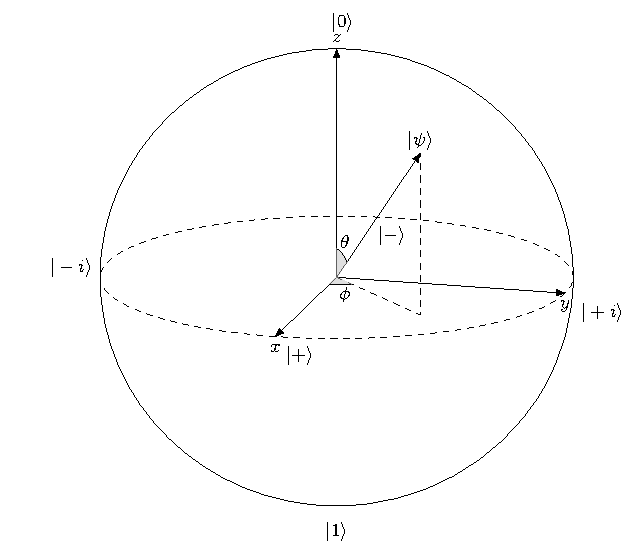
\includegraphics{figures/bloch_sphere.pdf}
\caption{The Bloch sphere, with the six Pauli eigenstates of Table~\ref{tab:pauli-eigenstates} labeled. Every single-qubit state is $\rho=\frac{1}{2}(\Id+\vec{r}\cdot(\sigma_x, \sigma_y, \sigma_z))$ with Bloch vector $\vec{r}\in\mathbb{R}^{3}$, $\norm{\vec{r}}\leq 1$, the \textit{Bloch ball}: pure states on the surface, mixed states inside.}
\label{fig:bloch-sphere}
\end{figure}

At the six intersections of the coordinate axes with the sphere sit the eigenstates of the three Pauli operators
\[
  \sigma_x = \begin{pmatrix} 0 & 1 \\ 1 & 0 \end{pmatrix}, \qquad
  \sigma_y = \begin{pmatrix} 0 & -i \\ i & 0 \end{pmatrix}, \qquad
  \sigma_z = \begin{pmatrix} 1 & 0 \\ 0 & -1 \end{pmatrix}.
\]
These eigenstates form three mutually unbiased bases~\cite{wootters1989optimalstatedeterminationmutually}, shown in Table~\ref{tab:pauli-eigenstates}. We denote the vector of Paulis $(\sigma_x, \sigma_y, \sigma_z)$ as $\sigmavec$. Together with the identity $\sigma_0 = \Id$, the three Pauli matrices form a basis for the real vector space of $2\times 2$ Hermitian matrices.

\begin{table}[h]
\centering
\renewcommand{\arraystretch}{1.05}
\begin{tabular}{cccc}
  \hline
  \textbf{Axis} & \textbf{State} & \textbf{Expansion} & $(\theta,\,\phi)$ \\
  \hline
  $+z$ & $\ket{0}$  & $\ket{0}$ & $(0,\;-)$ \\
  $-z$ & $\ket{1}$  & $\ket{1}$ & $(\pi,\;-)$ \\
  $+x$ & $\ket{+}$  & $\tfrac{1}{\sqrt{2}}\bigl(\ket{0}+\ket{1}\bigr)$ & $(\tfrac{\pi}{2},\;0)$ \\
  $-x$ & $\ket{-}$  & $\tfrac{1}{\sqrt{2}}\bigl(\ket{0}-\ket{1}\bigr)$ & $(\tfrac{\pi}{2},\;\pi)$ \\
  $+y$ & $\ket{+i}$ & $\tfrac{1}{\sqrt{2}}\bigl(\ket{0}+i\ket{1}\bigr)$ & $(\tfrac{\pi}{2},\;\tfrac{\pi}{2})$ \\
  $-y$ & $\ket{-i}$ & $\tfrac{1}{\sqrt{2}}\bigl(\ket{0}-i\ket{1}\bigr)$ & $(\tfrac{\pi}{2},\;\tfrac{3\pi}{2})$ \\
  \hline
\end{tabular}
\caption{Eigenstates of the Pauli operators and their Bloch sphere coordinates.
  These six states comprise three mutually unbiased bases for $\mathbb{C}^{2}$.}
\label{tab:pauli-eigenstates}
\end{table}

\subsubsection{Multiple Qubits}

The state space of $n$ qubits is the tensor product $\mathbb{C}^2 \otimes \cdots \otimes \mathbb{C}^2 \cong \mathbb{C}^{2^n}$ of the individual spaces; this finite-dimensional Hilbert space is the only one the thesis needs. The normalization condition reads $\braket{\psi}{\psi} = 1$, with $\bra{\psi} = \ket{\psi}^\dagger = (\ket{\psi}^*)^\top$ the Hermitian transpose of $\ket{\psi}$.

\subsubsection{Density Operators}

The \textit{density operator} $\rho$ (also called density matrix) of a state $\ket{\psi}$ is $\rho = \ketbra{\psi}{\psi}$; for representing the state of a system the two are equivalent. One may alternatively define the density operators as the positive operators $\rho$ on the state space that have trace\footnote{The \textit{trace} of a matrix---and any linear operator admits a matrix representation---is defined as the sum of its diagonal elements. For a matrix with entries $A_{ij}$ we define its trace as $\Tr[A] = \sum_{i} A_{ii}$.} one, $\Tr[\rho] = 1$. The formalism also covers probabilistic mixtures: an ensemble $\{p_i, \ket{\psi_i}\}$, the system being in state $\ket{\psi_i}$ with probability $p_i$, has density operator $\rho = \sum_{i} p_i \ketbra{\psi_i}{\psi_i}$. A \textit{mixed state} has $\Tr[\rho^2] < 1$, and a pure one has $\Tr[\rho^2] = 1$.

\subsection{Quantum Circuits: How To ``Run'' Something on a Quantum Computer} \label{sec:quantum_circuits}

A quantum computation is modeled as a quantum circuit: qubits are wires read from left to right, elementary gates are boxes on them, and a meter is a measurement; Figure~\ref{fig:tetrahedron-recipe} shows one, and Appendix~\ref{app:decker} five more. Wires start in $\ket{0}$ unless labeled otherwise: the all-zeros input $\ket{0}^{\otimes n}$ is the convention, and the state hardware prepares.

\subsubsection{Unitary Evolution, Gates}

It is a postulate of quantum mechanics that quantum states evolve through being acted on by unitary operators---\textit{unitary evolution}. In a circuit diagram, these appear as \textit{gates}. A unitary operator $U$ is such that $U^\dagger U = U U^\dagger = \Id$, where $U^\dagger$ is the Hermitian transpose $(U^*)^\top$, so that the normalization condition survives the evolution; on $n$ qubits, $U$ is a $2^n \times 2^n$ complex matrix. Geometrically, valid quantum gates correspond to rotations of the state vector on the hypersphere defined by the normalization condition: they change the direction of the state vector, never its length. While any unitary operation is a valid physical evolution, in practice any unitary we wish to implement will be decomposed (compiled) into a sequence of gates from a defined \textit{gate set}~\cite{nielsen2010quantumcomputationquantum}.

\subsubsection{Measurement, Readout}

Classical information leaves the computer through a \textit{measurement}, treated in more detail in Section~\ref{sec:measurement}; a circuit's readout is with respect to the computational basis, and returns a bitstring. Outcomes are random, and hardware is noisy, so even a deterministic circuit is executed repeatedly (``shots'') to build a statistical distribution of outcomes, and the readout data are post-processed, classically. A circuit acts on every branch of a superposition at once, but a measurement returns one outcome; out of the full, ``hidden'' information of a quantum system, we can only extract one measurement's worth. A challenge in designing quantum algorithms is arranging for that one measurement to, so to say, ``deliver the goods.''

\section{Measurement} \label{sec:measurement}

The description of the measurement is one of the fundamental postulates of quantum mechanics; we give it in its general form, and then as the POVMs the thesis is built on.

\subsection{General Measurements}

In the most general case, a measurement is a collection of measurement operators $\{M_m\}$, each associated with a measurement outcome $m$. When a measurement operator $M_m$ acts on a state $\ket{\psi}$ the probability of observing the associated outcome is $$p(m) = \bra{\psi}M_m^\dagger M_m \ket{\psi},$$ the post-measurement state being $M_m \ket{\psi} / \sqrt{p(m)}$, and the measurement must satisfy the \textit{completeness relation} $\sum_m{M_m^\dagger M_m} = \Id$, guaranteeing that the probabilities sum to 1.

\subsection{Projective Measurements}

Projective measurements arise when we restrict the general operators $\{M_m\}$ to satisfy Hermiticity and orthogonality,
\[
    M_m = M_m^\dagger, \qquad M_m M_{m'} = \delta_{mm'} M_m,
\]
where $\delta_{mm'}$ is the Kronecker delta; each $M_m = P_m$ is then a projector, Hermitian and \textit{idempotent} ($P_m^2 = P_m$). The $P_m$ project onto mutually orthogonal subspaces, and outcome $m$ has probability $p(m) = \bra{\psi} P_m \ket{\psi}$. A Hermitian operator $O = \sum_\lambda \lambda P_\lambda$, an \textit{observable}, defines one such measurement through its spectral decomposition, the outcome being the real eigenvalue $\lambda$. The ``meter'' symbol of Figure~\ref{fig:tetrahedron-recipe} stands for a projective measurement in the computational basis, i.e., $P_0 = \ketbra{0}{0}$ and $P_1 = \ketbra{1}{1}$.

\subsection{Positive Operator-Valued Measures (POVMs)}

When only the outcome statistics matter, and not the post-measurement state of the system, the POVM formalism is the useful one. A POVM is a collection of operators ${E_m}$, also referred to as \textit{effects}, such that $$E_m = M_m^\dagger M_m$$ for some general measurement $\{M_m\}$. The postulates of quantum mechanics then give us $$p(m) = \bra{\psi} E_m \ket{\psi} = \Tr[E_m \rho] \quad \text{and} \quad \sum_m E_m = \Id .$$

An alternative way to define the POVM $\{E_m\}$ is as a collection of \textit{positive}\footnote{A positive operator $E_m \ge 0$ is an operator such that $\bra{\psi} E_m \ket{\psi} \ge 0.$} operators $E_m \ge 0$ which satisfy the completeness relation $\sum_m E_m = \Id$.

The concrete realization of an arbitrary POVM is not trivial: the only directly realizable measurements are projective, and POVM effects need not be pairwise orthogonal. One route is Naimark’s dilation theorem~\cite[Thm.~2.42]{watrous2018theoryquantuminformation}: embed the POVM in a larger space, where the effects become orthogonal again (e.g., Section~\ref{subsec:deckercircuits}). The other, open only to some POVMs, is a classical mixture of projective measurements (Section~\ref{subsec:randomized-implementations}).
% Keep ``realization'' here: in this thesis the word is the mechanism-to-measurement relation, while ``implementation'' names the protocols (the three weighed in Chapter~\ref{cha:discussion}, two of them the randomized ones of Section~\ref{subsec:randomized-implementations}) and ``implementable'' carries the exactness claim (only the octahedron is exactly implementable). Swapping this one to ``implementation'' would assert a second implementability notion two chapters before that one is defined.

\section{Platonic Solids} \label{sec:platonic-solids}

The Platonic solids have been an object of geometric fascination for a very long time. First rigorously described by the ancient Greeks~\cite[Book~XIII]{euclid1956thirteenbookseuclids}, they have also been used in an attempt by \textcite{kepler1596prodromusdissertationumcosmographicarum} to build a model of the solar system. They continue to appear as useful objects of study in new contexts---such as quantum measurement~\cite{tavakoli2020platonicsolidsfundamental}. The Platonic solids are the tetrahedron with four vertices, the octahedron with six, the cube with eight, the icosahedron with twelve, and the dodecahedron with twenty; Figure~\ref{fig:platonic-solid-povms} draws all five on the Bloch sphere.

\subsection{Constructing the Solids: Definition} \label{subsec:constructing-solids}

The most succinct definition of a solid is through its Schl\"{a}fli symbol $\{p, q\}$, a convex polyhedron with regular $p$-gonal faces, $q$ meeting at each vertex~\cite{coxeter1973regularpolytopes}: the tetrahedron $\{3,3\}$, the cube $\{4,3\}$, the octahedron $\{3,4\}$, the icosahedron $\{3,5\}$, and the dodecahedron $\{5,3\}$ are the five integer solutions of $1/p + 1/q > 1/2$ with $p, q \geq 3$ (Appendix~\ref{app:rotations:schlafli}).

To obtain vertex coordinates in $\R^3$, one may compute the orbit of a seed vector under \textit{cyclic} permutations of coordinates and arbitrary sign flips. The tetrahedron is the four-vertex orbit of $(1,1,1)$ under \textit{even} sign flips alone, $\{(\pm 1, \pm 1, \pm 1) : xyz > 0\}$; the octahedron the orbit of $(0,0,1)$; and the cube the full orbit of $(1,1,1)$, namely all $(\pm 1, \pm 1, \pm 1)$. With the golden ratio $\phig = (1+\sqrt{5})/2$ and its inverse $\invphig = 1/\phig$, the icosahedron is the orbit of $(0,\phig,1)$, and the dodecahedron's twenty vertices are the union of the orbit of $(0, \invphig, \phig)$ with the cube.\footnote{Bare $\invphig$ is the inverse golden ratio, after Conway and Smith; Pauli matrices---always subscripted $\sigma_a$ or bolded $\boldsymbol{\sigma}$.}\footnote{The transposed seed $(0,1,\phig)$, also standard, generates the icosahedron's other vertex family (Appendix~\ref{sec:povm-atlas:families}).} Note that these seeds are unnormalized.

\subsection{Platonic Solids and Their Rotational Symmetry Groups}

The five Platonic solids come in dual pairs, the octahedron with the cube and the icosahedron with the dodecahedron, with the exception of the tetrahedron, which is self-dual. Their rotational symmetry groups, called the \textit{polyhedral groups}, are finite subgroups of the rotation group $\SO(3)$; Table~\ref{tab:permutation-structure} presents the details, adapted from work by \textcite{vanhoboken2002platonicsolidsbinary}. We denote as $\Tgroup$, $\Ogroup$, and $\Igroup$ the tetrahedral, octahedral, and icosahedral groups, respectively.

\subsection{Permutation Group Structure of Polyhedral Groups}

The rotational symmetry groups of the Platonic solids are isomorphic to well-known permutation groups, which provides an alternative way to understand their structure and action. The permutations of $n$ objects form the \textit{symmetric group} $S_n$, of order $n!$, and the even ones, products of an even number of transpositions, its \textit{alternating group} $A_n$, of order $n!/2$. We have the following three results.

The tetrahedral symmetry group $\Tgroup$ acts on the vertices of the tetrahedron by evenly permuting them, i.e., $\Tgroup$ is isomorphic to the group of even permutations of four elements $A_4$; Figure~\ref{fig:tetrahedron-recipe} lists all twelve, as permutations of the labeled vertices.

The octahedral symmetry group $\Ogroup$, while acting on the cube's eight vertices, and thus being embedded in $S_8$, can be seen to be acting on the four main diagonals of the cube. Since every rotation permutes the diagonals, and the action is faithful, only the identity fixing all four, we see that $\Ogroup \cong S_4$.

The icosahedral symmetry group $\Igroup$ can be examined as acting on five inscribed cubes in the dodecahedron. Any rotation of the dodecahedron takes an inscribed cube to another inscribed cube, permuting the set of five. We can examine each rotation type directly to see how the cubes will be permuted evenly, or make a structural argument to show that $\Igroup \cong A_5$~\cite[Thm.~7.4.4]{artin2011algebra}.

These results are compiled in Table~\ref{tab:permutation-structure}, together with each solid's vertex count $V$ and the design strength $t$ of its POVM (Section~\ref{subsec:tdesigns}). The parameters $(n_1, n_2, n_3)$ in the table are precisely $(p, q, 2)$, read from the Schl\"{a}fli symbol $\{p,q\}$ of each solid; more details in Appendix~\ref{app:rotations:schlafli}. The table returns in Section~\ref{sec:povmsinuse}, where its last row decides which group the dodecahedron's randomized implementation must draw from.

\begin{table}[H]
\centering
\begin{tabular}{cccccccc}
\toprule
Solid & $\{p,q\}$ & $(n_1, n_2, n_3)$ & Acts on & $|G|$ & $G$ & $V$ & $t$ \\
\midrule
Tetrahedron  & $\{3,3\}$ & $(3,3,2)$ & 4 vertices            & 12 & $\Tgroup \cong A_4$ & $\mathbf{4}$  & 2 \\
Octahedron   & $\{3,4\}$ & $(3,4,2)$ & 4 face-axes           & 24 & $\Ogroup \cong S_4$ & $\mathbf{6}$  & \multirow{2}{*}{3} \\
Cube         & $\{4,3\}$ & $(4,3,2)$ & 4 diagonals           & 24 & $\Ogroup \cong S_4$ & $8$           & \\
Icosahedron  & $\{3,5\}$ & $(3,5,2)$ & 5 edge-axis octahedra & 60 & $\Igroup \cong A_5$ & $\mathbf{12}$ & \multirow{2}{*}{5} \\
Dodecahedron & $\{5,3\}$ & $(5,3,2)$ & 5 inscribed cubes     & 60 & $\Igroup \cong A_5$ & $20$          & \\
\bottomrule
\end{tabular}
\caption{Permutation realizations of the polyhedral rotation groups~\cite{vanhoboken2002platonicsolidsbinary}, with each solid's vertex count $V$ and the design strength $t$ of its POVM (Section~\ref{subsec:tdesigns}). The triple $(n_1, n_2, n_3)$ records the face, vertex, and edge stabilizer orders (see Appendix~\ref{app:rotations:schlafli}). Dual pairs share the rotation group $G$, and $t$ is constant within each group block; bold $V$ marks a tight complex projective design, and the frame potentials behind $t$ are in Table~\ref{tab:povm-properties}.}
\label{tab:permutation-structure}
\end{table}

\section{The Binary Polyhedral Groups} \label{sec:binary-polyhedral-groups}

The algebra we need is standard~\cite{artin2011algebra}. A \textit{group} $G$ is a set with an associative composition, an identity $1$, and inverses; its \textit{order} $|G|$ is its number of elements, and a \textit{subgroup} $H \leq G$ is a subset closed under composition and inverses. For a subset $U \subseteq G$, $\langle U \rangle$ is the subgroup \textit{generated} by $U$, the smallest containing it, i.e., all products of elements of $U$ and their inverses; the bracket notation $\langle \cdot \rangle$ is slightly overloaded between this algebraic use, the Dirac inner product, and the expectation value, but context will always make our meaning clear. For $H \leq G$ and $a \in G$, the subset $aH = \{ah : h \in H\}$ is a \textit{left coset} of $H$; all left cosets of $H$ have $|H|$ elements and partition $G$. A \textit{homomorphism} $\varphi: G \rightarrow G'$ is a map with $\varphi(ab) = \varphi(a)\varphi(b)$; a bijective one is an \textit{isomorphism}, and $G \cong G'$ means one exists. Its \textit{kernel} $\ker\varphi = \{g \in G : \varphi(g) = 1\}$ is a subgroup, and the cosets of the kernel form a group, the \textit{quotient group} $G/\ker\varphi$, isomorphic to the image $\operatorname{im}\varphi = \varphi(G)$. The matrix groups we need are the \textit{unitary group} $\mathrm{U}(n)$ of complex $n \times n$ matrices with $U^\dagger = U^{-1}$, the abstract home of quantum gates; its determinant-one subgroup, the \textit{special unitary group} $\SU(n)$; and the \textit{rotation group} $\SO(n)$ of real matrices with $P^\top = P^{-1}$ and determinant one.

\subsection{Quaternions and the Isomorphism \texorpdfstring{$\SU(2) \cong \mathbb{H}_1$}{SU(2) ≅ H1}} \label{subsec:su2-h1}

Pure single-qubit states are vectors in $\C^2$ up to a global phase, with transformations governed by $\SU(2)$, and the discrete subgroups of $\SU(2)$ are best constructed through the unit quaternions~\cite{stillwell2008naivelietheory}. A \textit{quaternion} is written $q = w + xi + yj + zk$, with $w$, $x$, $y$, $z$ real coefficients and $i$, $j$, $k$ the basis elements; the quaternions $\mathbb{H}$ form a four-dimensional real vector space, and multiply by Hamilton's defining relation---famously cut in stone on the Brougham Bridge~\cite{vanderwaerden1976hamiltonsdiscoveryquaternions}:
$$ i^2 = j^2 = k^2 = ijk = -1, $$
from which $ij = k = -ji$, so that $\mathbb{H}$ is non-commutative, not a field. Given a quaternion $q$, its \textit{conjugate} $\bar{q}$ and \textit{norm} $\abs{q}$ are
$$ \bar{q} = w - xi - yj - zk, \qquad \abs{q}^2 = q \bar{q} = w^2 + x^2 + y^2 + z^2, $$
which give the multiplicative group of \textit{unit quaternions} $\mathbb{H}_1 = \{ q \in \mathbb{H} : \abs{q} = 1 \}$, in which $\bar{q} = q^{-1}$.

There is a fundamental isomorphism between $\SU(2)$ and the group of unit quaternions $\mathbb{H}_1$~\cite{stillwell2008naivelietheory}. A unit quaternion $q = w + xi + yj + zk$ maps to the unitary matrix
$$
U_q = \begin{pmatrix} w + ix & y + iz \\ -y + iz & w - ix \end{pmatrix} = w\Id + i\,(xZ + yY + zX).
$$
The constraint $\det(U_q) = 1$ requires $w^2 + x^2 + y^2 + z^2 = 1$, the 3-sphere $S^3 \subset \mathbb{R}^4$; and $q \mapsto U_q$ is multiplicative, so quaternions and unitaries are interchangeable in all algorithms of Chapter~\ref{cha:methods}. This $U_q$ and the seed coordinates of Section~\ref{subsec:constructing-solids} are two choices everything later is oriented by.

\subsection{The Double Cover \texorpdfstring{$\SU(2) \to \SO(3)$}{SU(2) → SO(3)}} \label{subsec:double-cover}

The matrix $U_q$ acts on the quantum state space and corresponds to a 3D rotation by angle $\theta = 2\arccos(w)$ about the Bloch axis $\hat n = -(z, y, x) / \sin(\theta/2)$, the na\"ive $(x, y, z)$ reversed and negated.\footnote{Two conventions map a quaternion to a rotation---the physics one we use here, and the standard math textbook one. The two \textit{do not agree}. Our definition of $U_q$ forces the quaternion units $i$, $j$, $k$ to be $\pi$ rotations about the Bloch $\hat z$, $\hat y$, $\hat x$ axes, in that order. The choice of convention matters. More in Appendix~\ref{sec:povm-atlas:families}.} The unitaries $U_q$ and $-U_q$ (corresponding to quaternions $q$ and $-q$) produce the same 3D rotation: structurally, the rotation is the conjugation action on the Bloch sphere, $\vec r \cdot \sigmavec \mapsto U_q\,(\vec r \cdot \sigmavec)\,U_q^\dagger$, in which $U_q$ enters twice---once daggered---so a global sign cancels. And only the sign cancels: any unitary acting trivially on the whole Bloch sphere commutes with all three Pauli matrices, hence is a scalar, and $\det = 1$ leaves exactly $\pm\Id$. This establishes the well-known 2-to-1 surjective homomorphism
$$ \phi: \SU(2) \to \SO(3), $$
with kernel $\ker\phi = \{\Id, -\Id\}$. Equivalently, $\SO(3) \cong \SU(2)/\{\pm\Id\}$.

The \textit{binary polyhedral groups} are defined as the preimages under $\phi$ of the rotational symmetry groups of the Platonic solids (Section~\ref{sec:platonic-solids}):
$$
\TwoT = \phi^{-1}(\Tgroup), \quad \TwoO = \phi^{-1}(\Ogroup), \quad \TwoI = \phi^{-1}(\Igroup).
$$
The double cover gives these groups twice the order of the corresponding polyhedral group. We call these groups \textit{exceptional}: the finite subgroups of $\SO(3)$ are the cyclic and dihedral groups together with $\Tgroup$, $\Ogroup$, and $\Igroup$~\cite{artin2011algebra}; the binary polyhedral groups lift the three exceptions. Geometrically, each is a point set on $S^3$: every $\SU(2)$ operator is uniquely identified with a 4D coordinate $(w, x, y, z)$ there, and Section~\ref{sec:construction4dpolytopes} constructs all three from the vertices of 4D polytopes. We write $\TwoG$ for any one of $\TwoT$, $\TwoO$, or $\TwoI$ when a statement applies uniformly to all three, with $\Ggroup$ the corresponding polyhedral group $\Tgroup$, $\Ogroup$, or $\Igroup$.

\section{The Platonic Solid POVMs} \label{sec:platonic-solid-povms}

With the binary polyhedral groups in hand, we can define the Platonic solid POVMs and examine them in detail. They are shown in Figure~\ref{fig:platonic-solid-povms}; a supplementary interactive visualization, \texttt{extras/povms.html}, is in the repository. We deal with the single-qubit case.

\begin{figure}[p]
  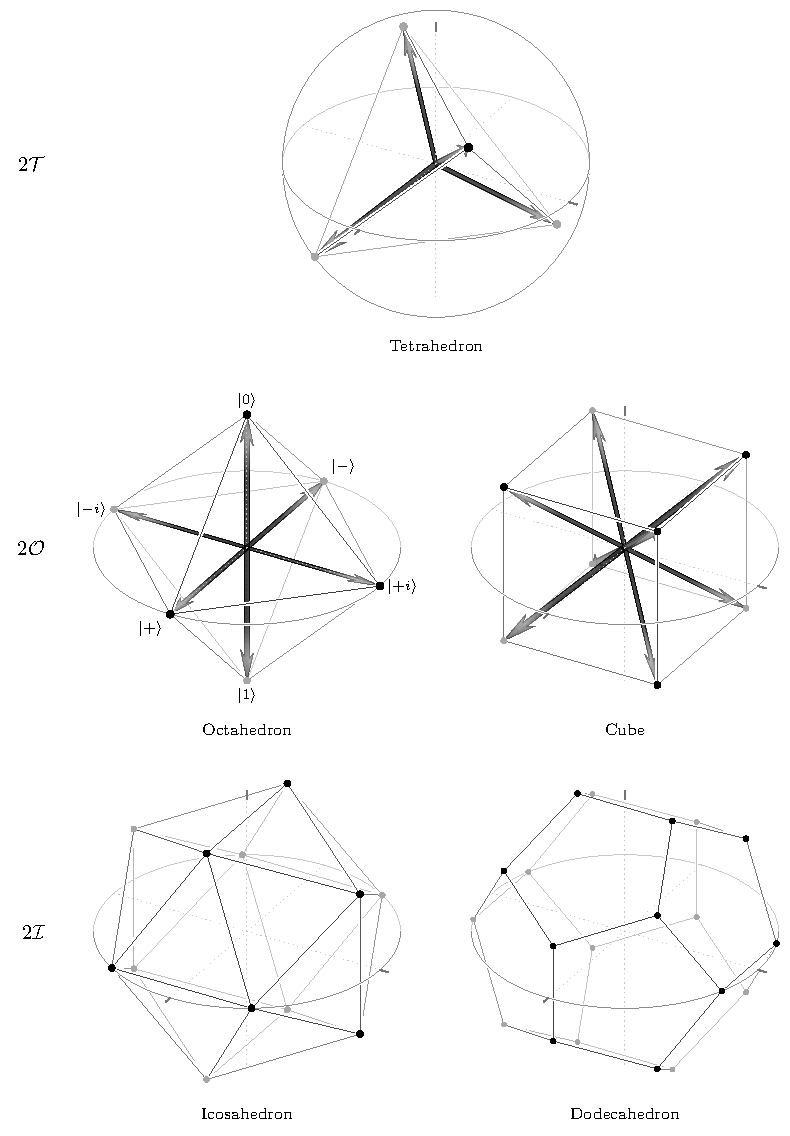
\includegraphics[width=0.95\textwidth]{figures/platonic_solid_povms.pdf}
  \caption{The five Platonic solid POVMs.}
  \label{fig:platonic-solid-povms}
\end{figure}

\subsection{Definition}

A Platonic solid POVM is a set of positive operators $E = \{ E_k \}_{k=1}^V$ defined by the vertices of a Platonic solid. For a solid with $V$ vertices described by unit vectors $\{ \hat{n}_k \} \subset \R^3$ on the Bloch sphere, the POVM elements are rank-1 projectors scaled to satisfy the completeness relation $\sum_k E_k = \Id$:
\begin{equation} \label{eq:povmform}
E_k = \frac{2}{V} \ketbra{\psi_k}{\psi_k} = \frac{2}{V} \frac12 \left( \Id + \hat{n}_k \cdot \sigmavec \right)
\end{equation}
A full list of coordinates can be found in Appendix~\ref{sec:povm-atlas:vertices}.

\subsection{Group-Covariant POVMs} \label{subsec:groupcovariantpovms}

\label{subsec:orbit-stabilizer}Groups become practically useful when they \textit{act} on something. An \textit{action} of a group $G$ on a set $S$ is a map $G \times S \rightarrow S$, $(g, s) \mapsto g \cdot s$, with $1 \cdot s = s$ and $(gg') \cdot s = g \cdot (g' \cdot s)$. The set $S$ can be anything: vertices of a polyhedron, basis vectors of a Hilbert space, or---most importantly for this thesis---indices of a measurement outcome. The \textit{orbit} of $s$ is $O_s = \{ g \cdot s : g \in G \}$, the orbits partition $S$, and the action is \textit{transitive} if $S$ is a single orbit, every $s$ sent to every other by some $g$; the \textit{stabilizer} $G_s = \{ g \in G : g \cdot s = s \}$ of $s$ is a subgroup. Given two actions of the same group $G$, on sets $X$ and $Y$, we may ask when a map between $X$ and $Y$ respects both. A map $f: X \rightarrow Y$ is \textit{$G$-equivariant} if
\begin{equation} \label{eq:equivariance}
  f(g \cdot x) = g \cdot f(x), \qquad \forall\, g \in G,\, x \in X.
\end{equation}

A POVM $\{E_k\}_{k=1}^V$ is \textit{group-covariant}~\cite{holevo2011probabilisticstatisticalaspects, decker2005implementationgroupcovariantpositive,chiribella2004extremalcovariantpositive} under a group $G$ with unitary representation $U: G \rightarrow \mathrm{U}(d)$, $g \mapsto U_g$ (a homomorphism; representations proper are Section~\ref{subsec:schur}'s), if there is an associated permutation action of $G$ on the indices $\{1, \dots, V\}$ such that
\[
  E_{g(k)} = U_g E_k U_g^\dagger \qquad \forall\, g \in G,\, k.
\]
This goes for any subgroup of such a $G$, so by the POVM's \textit{covariance group} we mean the largest in $\SU(2)$. Equivalently, the indexing map $k \mapsto E_k$ is $G$-equivariant~\eqref{eq:equivariance} between the permutation action on indices and the conjugation action on operators. This group action partitions the effects into one or more orbits. Covariance alone does not guarantee that every effect can be mapped to every other effect.

\subsection{Transitive Covariant POVMs}

A group-covariant POVM is \textit{transitive covariant}, or single-orbit covariant, if the group $G$ acts transitively on its effects. That is, for any two effects $E_i$ and $E_j$, there exists an element $g \in G$ such that:
$$ E_j = U_g E_i U_g^\dagger $$
Because the trace is invariant under cyclic permutation (and thus invariant under unitary conjugation $\Tr[U_g E_i U_g^\dagger] = \Tr[E_i]$), transitivity strictly implies that the POVM is \textit{equal-trace}, also called unbiased~\cite{liu2021relatingmeasurementdisturbance}: all effects have the same trace, which completeness fixes at $\Tr[E_k] = d / V$ in dimension $d$. The converse, however, does not universally hold: a POVM can be equal-trace and group-covariant while possessing multiple distinct orbits under the group action. Equal trace is one of the conditions for a POVM to be SIC (more on which in Section~\ref{subsubsec:tetrahedral-sic}), and is oft-overlooked, but strictly necessary~\cite{geng2021whatareminimal}.

\subsubsection{The Platonic solid POVMs are Transitive Covariant} \label{subsubsec:platonic-transitive}

Conjugating an effect $E_k = \frac{1}{V}(\Id + \hat{n}_k \cdot \sigmavec)$ by $U_g$ for any $g \in \TwoG$ gives
\[
U_g E_k U_g^\dagger = \frac{1}{V} \left( \Id + U_g (\hat{n}_k \cdot \sigmavec) U_g^\dagger \right) = \frac{1}{V} \left( \Id + (\phi(U_g)\, \hat{n}_k) \cdot \sigmavec \right),
\]
where $\phi(U_g) \in \SO(3)$ is the rotation corresponding to $U_g$ under the double cover (Section~\ref{subsec:double-cover}). Conjugation by $U_g$ for $g \in \TwoG$ thus rotates each POVM element's Bloch vector by $\phi(U_g)$. Since the polyhedral group $\Ggroup$ acts transitively on the vertices of its Platonic solid and $\TwoG$ covers $\Ggroup$, conjugation by $\TwoG$ acts transitively on the POVM's effects. The Platonic solid POVMs are therefore transitive covariant under $\TwoG$ (on the Bloch sphere, $\Ggroup$):
\[
  \{\, U_g E_k U_g^\dagger \,\}_{g \in \TwoG} = \{ E_k \}_k.
\]

For every $U \in \SU(2)$, conjugation carries the Bloch vector $\hat{n}_k$ to $\phi(U)\,\hat{n}_k$, and $\hat{n} \mapsto \frac{1}{V}(\Id + \hat{n} \cdot \sigmavec)$ is a bijection. So $U$ permutes the effects exactly when $\phi(U)$ maps the vertex set to itself---and a rotation doing that carries the vertices' convex hull, the solid itself (Section~\ref{subsec:constructing-solids}), to itself, hence lies in $\Ggroup$. Since $\TwoG = \phi^{-1}(\Ggroup)$ and $\ker\phi = \{\pm\Id\} \subset \TwoG$, the unitaries permuting the effects are precisely $\TwoG$: it is \textit{the} covariance group of Section~\ref{subsec:groupcovariantpovms}, not merely one of them.

\subsection{Representations and Schur's Lemma} \label{subsec:schur}

A \textit{representation} of a finite group $G$ on a finite-dimensional complex vector space $W$ is a group homomorphism $\pi: G \rightarrow \mathrm{GL}(W)$ into the invertible linear maps of $W$~\cite{serre1977linearrepresentationsfinite}; when $\pi$ is clear from context we write $g \cdot v$ for $\pi(g) v$, a representation being in particular a linear action of $G$ on $W$, and the unitaries $U_g$ of a covariant POVM are one. A subspace $W' \subseteq W$ is \textit{$G$-invariant} if $\pi(g) W' \subseteq W'$ for every $g \in G$; the subspaces $\{0\}$ and $W$ always are, and $(\pi, W)$ is \textit{irreducible} if $W \neq \{0\}$ and these two are its only $G$-invariant subspaces. Given representations $(\pi_1, W_1)$ and $(\pi_2, W_2)$ of $G$, a linear map $T: W_1 \rightarrow W_2$ is an \textit{intertwiner} if $T\, \pi_1(g) = \pi_2(g)\, T$ for all $g \in G$; equivalently, if $T$ is $G$-equivariant (Equation~\eqref{eq:equivariance}) with respect to the actions $\pi_1$ and $\pi_2$. We denote the space of intertwiners by $\mathrm{Hom}_G(W_1, W_2)$.

Schur's Lemma constrains the structure of intertwiners between irreducible representations. It is short to state, short to prove, and far-reaching: it is the mechanism by which symmetry forces an operator to be a scalar multiple of the identity. Let $(\pi_1, W_1)$ and $(\pi_2, W_2)$ be irreducible representations of a finite group $G$ over $\mathbb{C}$, and let $T \in \mathrm{Hom}_G(W_1, W_2)$. Then $T$ is either zero or an isomorphism; and if in addition $W_1 = W_2$ and $\pi_1 = \pi_2$, then $T = \lambda\, \Id$ for some $\lambda \in \mathbb{C}$.\footnote{By the intertwining condition, $\ker T$ is a $G$-invariant subspace of $W_1$ and $\operatorname{im} T$ one of $W_2$; irreducibility forces $\ker T \in \{ \{0\}, W_1 \}$ and $\operatorname{im} T \in \{ \{0\}, W_2 \}$, so a nonzero $T$ has $\ker T = \{0\}$ and $\operatorname{im} T = W_2$, an isomorphism. For the second claim, $T$ has an eigenvalue $\lambda \in \mathbb{C}$ since $W_1 = W_2$ is finite-dimensional over $\mathbb{C}$, and $T - \lambda \Id$ is an intertwiner with nontrivial kernel, so by the first part it is zero.}

A mild corollary, used next and again in Section~\ref{sec:single-qubit-noise}: when a representation $(\pi, W)$ decomposes as $W = \bigoplus_i W_i$ into pairwise non-isomorphic irreducible subrepresentations, any self-intertwiner $T \in \mathrm{Hom}_G(W, W)$ is diagonal in that decomposition, acting as a scalar on each $W_i$. (The cross terms $W_i \to W_j$ for $i \neq j$ vanish by the first claim of the lemma; the diagonal restrictions are scalars by the second.)

\subsection{Stabilizer Subgroups and Commutation}

For a group-covariant POVM, we can examine the symmetry of individual effects. The stabilizer $G_k = \{ h \in G : h(k) = k \}$ of an index $k$ fixes its effect, so covariance restricted to $h \in G_k$ reads
$$ E_k = E_{h(k)} = U_h E_k U_h^\dagger \quad \forall h \in G_k, $$
and multiplying on the right by $U_h$ gives the commutation relation $E_k U_h = U_h E_k$. Every effect $E_k$ thus commutes with $U_h$ for every $h$ in its stabilizer $G_k$: it is a self-intertwiner of the stabilizer's representation, so the corollary to Schur's Lemma (Section~\ref{subsec:schur}) forces $E_k$ to act as a scalar on each irreducible piece of that representation. On the Bloch sphere, $G_k$ acts as the rotations about the vertex $\hat n_k$, so $U_h$ and $E_k$ alike are diagonal in the eigenbasis of $\hat n_k \cdot \sigmavec$: Equation~\eqref{eq:povmform}'s form. This greatly simplifies the estimation of observables from measurement~\cite{nguyen2022optimisingshadowtomography}: reconstruction reduces to the per-solid constants of Table~\ref{tab:shadow-reconstruction}. In this context, transitivity and this restriction are called \textit{uniformity} and \textit{rigidity}~\cite{nguyen2020symmetriesmeasurementsquantum}.

\subsection{Informational Completeness}

A POVM is \textit{informationally complete} (distinct states give distinct outcome distributions) when its effects span the real vector space of Hermitian operators on $\C^d$. For the single-qubit, rank-1 form of Equation~\eqref{eq:povmform} this 4-dimensional space is spanned by $\{\Id, \sigma_x, \sigma_y, \sigma_z\}$, and the condition reduces to the Bloch vectors $\{\hat n_k\}$ spanning $\R^3$. All Platonic solid POVMs are informationally complete (IC-POVMs). In fact, they satisfy the stronger condition
$$ \frac{1}{V} \sum_k \ket{\psi_k}\bra{\psi_k}^{\otimes 2} = \frac{1}{6} (\Id^{\otimes 2} + \operatorname{SWAP}_{12}),$$
with $\operatorname{SWAP}_{12}$ the \textit{swap operator} exchanging the two tensor factors of $(\C^2)^{\otimes 2}$; this characterizes the POVMs as complex projective $2$-designs, in the sense of Section~\ref{subsec:tdesigns}. Loosely, we may view this operator as swapping wires in a circuit diagram, but it is better thought of as the representation of $(1\ 2) \in S_2$. The two checks are verified in Appendix~\ref{sec:povm-atlas:ic}.

\subsection{Spherical vs.\ Complex Projective \texorpdfstring{$t$}{t}-designs} \label{subsec:tdesigns}

It is in their properties as \textit{designs} that the Platonic solid POVMs can be more usefully distinguished. We make sure to carefully note what \textit{kind} of design is formed by which solid, living in which space. A third kind, over the groups rather than the solids, waits until Section~\ref{subsec:unitary-designs}.

\subsubsection{Spherical Designs}

A finite non-empty set of vectors $\mathcal{V}$ on the unit sphere $S^{d-1}$ of the $d$-dimensional Euclidean space $\mathbb{R}^d$ is a \textit{spherical} $t$-design if, for any polynomial $f \in \mathbb{R}[x_1, \dots, x_d]$ of degree $\leq t$, we have
$$ \frac{1}{|S^{d-1}|} \int_{S^{d-1}} f(x) \, d\Omega(x) = \frac{1}{|\mathcal{V}|} \sum_{v \in \mathcal{V}} f(v) $$
where $\Omega$ is the surface measure on $S^{d-1}$ and $|S^{d-1}| = \int_{S^{d-1}} d\Omega(x)$~\cite{hirao2025sphericaldesignsfinite}. The concept was first introduced by \textcite{delsarte1977sphericalcodesdesigns}. The maximum value of $t$ for a given $\mathcal{V}$ is known as its \textit{design strength}. A $t$-design is \textit{tight} if it uses the minimum possible number of points for that particular value of $t$; such designs are rare, and difficult to classify~\cite{nasmith2023tight}.

\subsubsection{Complex Projective Designs}

Of more relevance is the extension of the concept of a spherical design to the complex projective space $\mathbb{CP}^{d-1}$, whose elements are unit vectors $\ket{v}$ in $\C^d$ up to global phase, equivalently the rank-1 projectors $\ketbra{v}{v}$. A finite set of vectors $\mathcal{V}$ (such as those forming a POVM) are a complex projective $t$-design if the following relation holds:
$$ \frac{1}{|\mathcal{V}|} \sum_{v \in \mathcal{V}} (\ketbra{v}{v})^{\otimes t} = \binom{d+t-1}{t}^{-1} \Pi_{\mathrm{sym}}^{(t)} $$
where $\Pi_{\mathrm{sym}}^{(t)}$ is the projector onto the totally symmetric subspace of $(\C^d)^{\otimes t}$, the states fixed by every permutation of the tensor factors~\cite{scott2006tightinformationallycomplete, roy2007weightedcomplexprojective, harrow2013churchsymmetricsubspace}. (For $t=1$: $\Pi_{\mathrm{sym}}^{(1)} = \Id_d.$ For $t=2$: $\Pi_{\mathrm{sym}}^{(2)} = \frac{1}{2}(\Id + \operatorname{SWAP}_{12}).$ We refer to the literature for more details~\cite[Ch.~7]{watrous2018theoryquantuminformation}.)

Alternatively, the Welch bounds~\cite{welch1974lowerboundsmaximum}, stated in terms of the average squared overlap, are saturated for all $k \leq t$ if and only if the set of vectors is a $t$-design in $\mathbb{CP}^{d-1}$~\cite{klappenecker2005mutuallyunbiasedbases, datta2012geometrywelchbounds,belovs2008criterionattainingwelch}. That is, the \textit{frame potential}
$$ \Phi_t(\mathcal{V})=\frac{1}{|\mathcal{V}|^2}\sum_{i,j} |\braket{\psi_i}{\psi_j}|^{2t}$$ saturates the bound
$$\Phi_t\ge \binom{d+t-1}{t}^{-1}.$$

Each Platonic solid POVM's design strength $t$, decided by this Welch bound computation with the vertex count $V = |\mathcal{V}|$, is in Table~\ref{tab:permutation-structure}, spherical and projective strength agreeing throughout; the frame potentials are printed once, in Table~\ref{tab:povm-properties} of Appendix~\ref{sec:povm-atlas:designs}.

\subsection{Special Cases}

The Platonic solid POVMs have received much study---some more than others. In particular, the tetrahedral and octahedral POVMs are well-known; more recently, the binary icosahedral group $\TwoI$ underlying the icosahedral POVM has received some attention as a fault-tolerant gate set~\cite{parzanchevski2018supergoldengatespu2, kubischta2023familyquantumcodes,kubischta2024quantumcodestwisted,zhang2025transversalgatesnonadditive}. We cover the exceptional solid per group below.

\subsubsection{Tetrahedral} \label{subsubsec:tetrahedral-sic}

The tetrahedron is a spherical 2-design, a complex projective 2-design, and tight. The tetrahedral POVM is the usual example of a Symmetric Informationally Complete POVM (SIC-POVM)~\cite{renes2004symmetricinformationallycompletea}: $d^2$ rank-1 effects $E_i \propto \ketbra{\psi_i}{\psi_i}$ with constant pairwise overlap $|\braket{\psi_i}{\psi_j}|^2 = 1/(d+1)$. \textit{Symmetric}, as the equal overlaps mean no pair of outcomes is favored, and are exactly what saturate the Welch bound $\Phi_2 = 1/3$ of Table~\ref{tab:povm-properties}. Geometrically, for $d = 2$ they force a regular tetrahedron---unique up to rotation. \textit{Informationally complete}: at $d^2 = 4$ effects, it is IC with the fewest outcomes possible~\cite{geng2021whatareminimal}. Whether SICs exist in every dimension---\textit{Zauner's conjecture}---remains a famous open problem~\cite{zauner2011quantumdesignsfoundations}. Moreover, the tetrahedral POVM is \textit{indecomposable}: alone among the five, it is not a classical mixture of other measurements, projective or not~\cite{dariano2005classicalrandomnessquantum}. It has been implemented as a single setting on real hardware~\cite{stricker2022experimentalsinglesettingquantum}.

\subsubsection{Octahedral}

The octahedral POVM is the classical example of a set of Mutually Unbiased Bases (MUB): orthonormal bases such that a state prepared in one basis, measured in another, gives every outcome with equal probability $1/d$. Its six Bloch vectors are exactly the Pauli eigenstates of Table~\ref{tab:pauli-eigenstates}, read as the maximal set of MUBs in $d = 2$---thus also a complex projective 2-design~\cite{klappenecker2005mutuallyunbiasedbases}. In fact, as the set of qubit stabilizer states for $n = 1$, it is actually a 3-design~\cite{kueng2015qubitstabilizerstates}---and tight. It has been implemented as a single setting on real hardware~\cite{an2024efficientcharacterizationsmultiphoton}.

\subsubsection{Icosahedral}

The icosahedron is the unique tight spherical 5-design on $S^2$~\cite[Example~5.16]{delsarte1977sphericalcodesdesigns}, and a tight complex projective 5-design on $\mathbb{CP}^1$, where it is rather exceptional: it is a counterexample to \textcite{hoggar1989tight45designs}'s proposed bounds on the existence of tight $t$-designs; \textcite{lyubich2007tightprojectivedesigns} repaired the proof by showing it is the unique case in $\mathbb{CP}^1$ whose angle set is not rational.

\section{Single-Qubit Noise} \label{sec:single-qubit-noise}

We've worked so far in the ideal case---unitary evolution, faithful readout. A real apparatus adds noise, and single-qubit noise can be modeled elegantly. The most general evolution of a quantum state is a completely positive trace-preserving map, a \textit{channel}~\cite[Ch.~8]{nielsen2010quantumcomputationquantum}, and on one qubit every channel acts on the Bloch vector $r$ as an affine map
$$ r \mapsto Tr + t, $$
with $T$ a real $3 \times 3$ matrix and $t \in \R^3$ a shift~\cite[App.~A.2]{acharya2021informationallycompletepovmbased}. The matrix distorts the ball---shrinking, rotating, squashing---and the shift displaces it, complete positivity bounding how far either can go and enforcing physicality. (This $T$ is the noise's matrix, not the $T$-gate; this $t$ is a shift, not a design strength.)

Three kinds of noise will come up, all diagonal in the Bloch basis $\hat x$, $\hat y$, $\hat z$, i.e., each axis maps into itself, none leaks into another, and the one shift points along $\hat z$. \textit{Depolarizing} noise at rate $p$ contracts the ball uniformly, $T = (1-p)\Id$, $t = 0$. \textit{Dephasing} at rate $p$ applies $\sigma_z$ with probability $p$, $T = \mathrm{diag}(1-2p,\, 1-2p,\, 1)$, $t = 0$: the equator contracts, nothing along the $\hat z$-axis moves. \textit{Amplitude damping} at rate $\gamma$ models decay toward $\ket{0}$, $T = \mathrm{diag}(\sqrt{1-\gamma},\, \sqrt{1-\gamma},\, 1-\gamma)$, $t = (0, 0, \gamma)$: the ball deforms and rides up the $\hat z$-axis. Dephasing and amplitude damping both fix $\ket{0}$, i.e., $T\hat z + t = \hat z$, so probing for noise via preparing $\ket{0}$ states cannot see them.

This invites a symmetry attack. Draw a rotation $R_g$ uniformly from a finite subgroup $G$ of $\SO(3)$. Conjugate the channel by it---apply the rotation, let the noise act, undo the rotation---and then average over the draw. The channel is \textit{twirled}:
$$ T \mapsto \frac{1}{|G|} \sum_{g \in G} R_g^\top\, T\, R_g, \qquad t \mapsto \frac{1}{|G|} \sum_{g \in G} R_g^\top\, t. $$
The averaged matrix commutes with every rotation in $G$ (re-index the sum), so if $G$ acts irreducibly on $\R^3$ the corollary to Schur's Lemma (Section~\ref{subsec:schur})---its intertwiner $T$, here in the flesh---forces it to be $\lambda \Id$;\footnote{The lemma was stated over $\C$, where every operator has an eigenvalue; a real matrix need not. Odd dimension rescues the argument: the characteristic polynomial of the averaged $T$ is a real cubic, so it has a real root $\lambda$, and $T - \lambda\Id$ is again an intertwiner, its kernel a nonzero invariant subspace that irreducibility makes all of $\R^3$.} conjugation preserves the trace, so the scalar is $\lambda = \Tr[T]/3$, and the $G$-twirl of \textit{any} noise is exactly depolarizing. The averaged shift dies outright: re-indexing again shows it is fixed by every rotation in $G$, and a nonzero fixed vector would span an invariant line, which irreducibility forbids. This collapse is why the groups of this thesis, all acting irreducibly, can promise depolarizing noise as a theorem---to be discussed in Chapter~\ref{cha:discussion}.

Noise numbers come on two scales: the quantum channel's and the lab data's. The matrix $T$ and the scalar $\Tr[T]/3$ belong to the channel; with no noise they are $\Id$ and $1$. The observable estimators of Chapter~\ref{cha:discussion} and Appendix~\ref{app:shadows} never see the channel directly. They see it through a measurement, and the measurement scales things too. Measure an ideal Platonic solid POVM repeatedly on a state with Bloch vector $r$ and average the observed vertices: the mean is not $r$ but $r/3$, forced by the $2$-design property of Section~\ref{subsec:tdesigns}, a geometric consequence. A scalar estimated from data (a calibration) therefore carries that third, and with \textit{no} noise it reads $1/3$. The two scales, a factor of $3$ apart, both return later. When in doubt, ask what the number would read with no noise at all: $1$ is the channel's scale, $1/3$ a calibration's.

\chapter{Methods} \label{cha:methods}

Two questions are answered in this chapter. What the group elements are, we answer twice over, from minimal quaternion generators and from 4D polytope vertices. Seeking to run them on a quantum computer leads us to canonical gate generators---an exact gate sequence for every element. We compile, then, as well as construct.

\section{Finding the Elements: Quaternion Generators and 4D Polytopes} \label{sec:constructingthebpg}

\textcite[\S3.5]{conway2009quaternionsoctonionstheir} give each binary polyhedral group a minimal generating set within the quaternions, a shared generator $\zeta$ (their $\omega$) together with one group-specific generator:
\[
    \TwoT = \langle i, \zeta \rangle, \quad \TwoO = \langle \frac{j+k}{\sqrt{2}}, \zeta \rangle, \quad \TwoI = \langle \frac{i + \invphig j + \phig k}{2}, \zeta \rangle, \qquad \zeta = \frac{-1+i+j+k}{2}.
\]
From there, a breadth-first (BFS) closure, multiplying known elements by the generators until nothing new appears, is guaranteed to produce exactly 24 elements for $\TwoT$, 48 for $\TwoO$, and 120 for $\TwoI$ (\texttt{conway\_group} in the repository's \texttt{main.py}).

\label{sec:construction4dpolytopes}The 24, 48, and 120 elements of $\TwoT$, $\TwoO$, $\TwoI$ are also exactly the vertex sets of three highly symmetric 4D configurations: the 24-cell, its union with its dual, and the 600-cell~\cite{coxeter1973regularpolytopes, dechant2013platonicsolidsgenerate}. In particular, the 24-cell and 600-cell are regular 4D polytopes, with Schl\"{a}fli symbols $\{3,4,3\}$ and $\{3,3,5\}$. Under $(a, b, c, d) \mapsto a + bi + cj + dk$, a finite set of points on $S^3 \subset \mathbb{R}^4$ closed under quaternion multiplication is a finite subgroup of $\SU(2)$, so explicit vertex coordinates (Appendix~\ref{app:rotations:coordinates}) construct the groups directly. The 600-cell is the 24-cell plus 96 vertices, the even coordinate permutations of the base coordinate $(\pm 1, \pm \phig, \pm \invphig, 0)/2$, an inclusion we will see in the quantum context.

\section{Compiling Them: Canonical Gate Generators}

While the quaternionic generators are algebraically elegant, we ultimately wish to work with these groups in the context of quantum information. To this end, we can define them via sets of \textit{canonical} quantum gate generators~\cite{kubischta2023familyquantumcodes}.

\subsection{Working in SU(2)} \label{sec:workinginsu2}

It is common in quantum computing to ignore global phases, treating the single-qubit quantum gates as living in $\PU(2) = \U(2)/\U(1)$, leading to the intuition that a $2\pi$ rotation on the Bloch sphere is the identity ($Z^2 = \Id$). A crucial distinction must be made for the binary polyhedral group unitaries, which we will treat as living in $\SU(2)$.

The binary polyhedral groups are subgroups of the unit quaternions $\mathbb{H}_1 \cong S^3 \cong \SU(2)$, which form the double cover of $\SO(3) \cong \SU(2)/\{\pm\Id\} \cong \PU(2)$. In this setup, a $2\pi$ rotation corresponds to $-\Id$, requiring a $4\pi$ rotation to return to identity. To maintain the group structure, all gates must be symmetrized to have determinant $+1$.

To generate these groups correctly, we must use the \textit{symmetrized gates}~\cite{kubischta2023familyquantumcodes}, defined as:
\[
\mathbf{X} = -i X, \quad \mathbf{Z} = -i Z, \quad \mathbf{H} = -i H, \quad \mathbf{S} = e^{-i\pi/4} S, \quad \mathbf{F} = \mathbf{H}\mathbf{S}^\dagger
\]
These definitions ensure that $\det(U) = 1$ for all generators. For example: $\mathbf{Z}^2 = (-iZ)^2 = -\Id$.

\subsection{Canonical Generators} \label{sec:canonicalgenerators}
Following \textcite{kubischta2023familyquantumcodes}, the binary tetrahedral group $\TwoT$ is generated by the symmetrized facet gate $\mathbf{F}$, along with symmetrized Paulis; the binary octahedral group $\TwoO$ \textit{is}---in $\SU(2)$---the single-qubit Clifford group $\mathcal{C}_1$, the normalizer of $\langle \mathbf{X}, \mathbf{Z} \rangle$; and the binary icosahedral group $\TwoI$ is generated by adding the \textit{golden gate} $\Phi$:
$$ \TwoT = \langle \mathbf{X}, \mathbf{Z}, \mathbf{F} \rangle, \qquad \TwoO = \langle \mathbf{X}, \mathbf{Z}, \mathbf{F}, \mathbf{H}, \mathbf{S} \rangle, \qquad \TwoI = \langle \mathbf{X}, \mathbf{Z}, \mathbf{F}, \Phi \rangle. $$
The golden gate $\Phi$ is defined in terms of the golden ratio $\phig$, and we may also define the gate $\Phi^\star$ in terms of the inverse golden ratio $\invphig$ to get:
\begin{equation}\label{eq:golden-gate}
    \Phi = \frac{1}{2} \begin{pmatrix} \phig + i\phig^{-1} & 1 \\ -1 & \phig - i\phig^{-1} \end{pmatrix}, \quad \Phi^\star = \frac{1}{2} \begin{pmatrix} -\invphig - i\invphig^{-1} & 1 \\ -1 & -\invphig + i\invphig^{-1} \end{pmatrix},
\end{equation}
which lets us alternatively generate $\langle \mathbf{X}, \mathbf{Z}, \mathbf{F}, \Phi^\star \rangle$---a second group, isomorphic to $\TwoI$, though not the same.\footnote{Our $\Phi^\star$ is the entry-wise image of $\Phi$ under $\sqrt{5} \mapsto -\sqrt{5}$; \textcite{kubischta2023familyquantumcodes} additionally take a complex conjugate---giving $\mathbf{Z} \Phi^{\star\dagger} \mathbf{Z}^\dagger$---but both generate the same target. The choice is cosmetic; more in Section~\ref{sec:constructionrelationship}.}\footnote{Plain or superscripted, $\Phi$ is the golden gate; subscripted, $\Phi_t$ is always a frame potential.}

BFS over these gates then generates each group as gate sequences, minimizing total circuit depth (Appendix~\ref{app:synthesis}). Inverses are in the initial generating set, and the facet gate counts as one primitive, depth-1.

\subsection{Algorithm: \texorpdfstring{$\Phi$}{Φ}-Aware Dijkstra} \label{sec:magicawaredijkstra}

A standard breadth-first search treats all generators as equal cost. For $\TwoI$, however, $\Phi$ is an exotic resource, whereas the gates $\{\mathbf{X}, \mathbf{Z}, \mathbf{F}\}$ that generate $\TwoT$ are cheap Clifford gates. The left-coset decomposition $\TwoI = \bigsqcup_{k=0}^4 \Phi^k (\TwoT)$ already implies that every element needs at most four $\Phi$ gates, all at the start of the circuit~\cite{kubischta2023familyquantumcodes}, but read naively, with generators restricted to positive powers, it spends $\Phi^4$ where $\Phi^{-1}$ (itself $\mathbf{X} \Phi \mathbf{X}^\dagger$: one $\Phi$ in a Pauli jacket) will do.

Instead, we perform a shortest-path search on the Cayley graph of~$\TwoI$. The vertices of this graph are the group elements; for each generator $g$ and each vertex $v$ there is a directed edge $v \to vg$. We assign each edge a cost
\begin{equation*}
    c(g) =
    \begin{cases}
        0 & g \in \{\mathbf{X},\, \mathbf{Z},\, \mathbf{F},\, \mathbf{H},\, \mathbf{S}\} \cup \{\text{all adjoints}\}, \\[4pt]
        1 & g \in \{\Phi,\, \Phi^\dagger\},
    \end{cases}
\end{equation*}
so that the total cost of a gate sequence $g_1 g_2 \cdots g_d$ is its \textit{$\Phi$-count}, the number of non-Clifford gates it contains~\cite{mooney2021costoptimalsinglequbitgate}. (For the Clifford${}+T$ set, $T = \mathrm{diag}(1, e^{i\pi/4})$, the same count is the $T$-count. We discuss $\Phi$ \textit{itself} in Appendix~\ref{app:synthesis}.) Each search runs over its group's generator set, adjoints included, so that $\mathbf{Z}^{-1}$ is reached directly as $\mathbf{Z}^\dagger$ (depth~1) rather than as $\mathbf{Z}^3$ (depth~3).
% The thesis prints $\Phi$-count throughout; the code and the npz keys keep the older name ``magic cost'', and the repository's readme carries the dictionary.

The optimization target is \textit{lexicographic}: we first minimize the $\Phi$-count~$m$, then, among sequences of equal $\Phi$-count, minimize the circuit depth~$d$. We write $(m', d') \prec (m, d)$ when $m' < m$, or $m' = m$ and $d' < d$. This is the ordering that Algorithm~\ref{alg:dijkstra_gen} exploits.

\begin{algorithm}[H] %
\caption{$\Phi$-aware synthesis via Dijkstra's algorithm}
\label{alg:dijkstra_gen}
\begin{algorithmic}[1]
\Require Generator set $S$ with costs $c(g)$; target set $T \subseteq \TwoI$
\Ensure For each $U \in T$: an optimal gate sequence, its $\Phi$-count $m$, and its depth $d$
\State Initialize the search frontier $\mathcal{Q} \gets \{(\,0,\; 0,\; \Id,\; \varepsilon\,)\}$
    \Comment{Each entry is $(m,\, d,\, U,\, \text{sequence})$}
\State Initialize visited map $\mathcal{V} \gets \{\Id \mapsto (0, 0)\}$
\While{$\mathcal{Q} \neq \varnothing$ and not all targets found}
    \State Extract the entry $(m,\, d,\, U,\, w)$ from $\mathcal{Q}$ with minimal $(m, d)$
    \If{$U \in T$ and $U$ not yet recorded}
        \State Record $(w, m, d)$ for $U$ \Comment{We've obtained the end result for $U$.}
    \EndIf
    \For{each $g \in S$}
        \State $U' \gets U \cdot g$, \quad $m' \gets m + c(g)$, \quad $d' \gets d + 1$
        \If{$(m', d') \prec \mathcal{V}[U']$}
            \State Update $\mathcal{V}[U'] \gets (m', d')$
            \State Insert $(m',\, d',\, U',\, w \cdot g)$ into $\mathcal{Q}$
        \EndIf
    \EndFor
\EndWhile
\end{algorithmic}
\end{algorithm}

Because every Clifford edge has zero weight, the algorithm exhausts the full Clifford orbit (i.e., the $\TwoT$ coset) at each $\Phi$-count before advancing to the next. For the all-Clifford groups $\TwoT$ and $\TwoO$ the search reduces to an ordinary breadth-first search that minimizes depth alone.

We run each search once in $\SU(2)$, and once in $\PU(2)$, where $q$ and $-q$ are one vertex.

\section{Implementation Details} \label{sec:implementationdetails}

All computation is symbolic, in Python with SymPy~\cite{meurer2017sympysymboliccomputing}. Quaternion components are expressions over $\mathbb{Q}(\sqrt{2}, \sqrt{5})$---rationals, $\sqrt{2}$, and the golden ratio $\phig$---with no floating-point approximation at any stage. Closure and equality are exact. Code is in \texttt{code/main.py}, with a notebook alongside. %

Three independent checks establish correctness. First, the algebraic closure of the Conway--Smith generators and the 4D polytope vertices produce identical element sets, of orders 24, 48, and 120. Second, every synthesized sequence is replayed symbolically and compared against its target quaternion: exact in $\SU(2)$, up to sign ($q \equiv -q$) in $\PU(2)$. Third, \texttt{code/numpy\_atlas.py} re-derives the groups, synthesis, and POVMs in NumPy.

\subsection{Normal Form Comparison}

SymPy's \texttt{simplify} is a heuristic, not a normal form: two expressions denoting the same algebraic number need not reduce to the same tree---for rich enough expression classes, zero-testing is outright undecidable~\cite{richardson1968undecidableproblemsinvolving}. Hashing simplified expressions could then let a search visit the same group element twice, silently corrupting group orders and shortest sequences. But every quaternion component lies in $\mathbb{Q}(\sqrt{2}, \sqrt{5})$, uniquely $a + b\sqrt{2} + c\sqrt{5} + d\sqrt{10}$ with rational $a, b, c, d$; reduction to this $4$-tuple is a canonical form, on which equality comparison and hashing are well-behaved. Sixteen ordered rational numbers per quaternion. Equality and membership checks run on hashes of these tuples, and never rely on \texttt{simplify}.

\subsection{Global Phase Tracking}

Each symmetrized gate is $\mathsf{G}_{\SU(2)} = \varphi_\mathsf{G} \, \mathsf{G}_{\U(2)}$ for a known phase factor $\varphi_\mathsf{G}$, with an adjoint carrying $\overline{\varphi_\mathsf{G}}$. Being complex scalars, phase factors pull out of a product. An $\SU(2)$ search match pins the symmetrized product to $q$, a $\PU(2)$ match to $\pm q$, the target quaternion up to a sign. A sequence of standard gates therefore multiplies out to $\varphi \, U_q$ with $\varphi = \pm \big(\prod_\mathsf{G} \varphi_\mathsf{G}\big)^{-1}$, the sign $+$ if the symmetrized product is $U_q$ and $-$ if it is $-U_q$.

Recording $\varphi$ is what turns the bold letters of the atlas into an exact $\U(2)$ identity for the standard ones a device runs, and tracks which of $\pm q$ a standard-gate circuit lands on. Computing $\varphi$ is also verification: it forces a comparison against both $+q$ and $-q$ that'd otherwise not run. Finally, called as a controlled subroutine, a gate turns its unobservable global phase into an observable relative one (we study no controlled $U_q$; the preamble of Appendix~\ref{app:atlas} gives the control's correction). In all cases, $\varphi$ is an 8th root of unity $\omega^k$, with $\omega = e^{i\pi/4}$.

\subsection{Antipodal pairing}

Elements are grouped into antipodal pairs $(q, -q)$, reflecting the double cover. Both members map to the same $\PU(2)$ element, so the atlas prints the Bloch rotation only once per pair; each row keeps its \textit{own} $\SU(2)$ sequences and phases---though \textit{either} row's sequence serves both members, as $\varphi U = (-\varphi)(-U)$.
Each pair is keyed by the lexicographically smaller of the two canonical coefficient tuples (those of $q$ and of $-q$), hashed---a sign-invariant key that is deterministic across runs.

\section{Three Routes, One Anchored Group Copy} \label{sec:constructionrelationship}

The routes differ in their starting points---minimal quaternion generators, explicit 4D coordinates, quantum gates---not in the elements they reach: the Conway--Smith closure computes precisely the vertices of the 24-cell, its union with its dual, and the 600-cell; the gate-generated unitaries are the same quaternions once more, seen through $\mathbb{H}_1 \cong \SU(2)$. Stronger than a group isomorphism, we have \textit{equality}, element for element. Section~\ref{sec:implementationdetails} verifies it as such: identical element sets for the two constructions, a replayed gate sequence for every element for the compilation.

That the gates generate precisely the Conway--Smith quaternions is a \textit{choice}. Abstractly, $\SU(2)$ contains infinitely many conjugate copies $u\,\TwoG\,u^{-1}$ of each binary polyhedral group. Rotate the 600-cell about the vertex $1$ (the identity quaternion) and its vertices still form a group isomorphic to $\TwoI$: a rotation of $S^3$ fixing the point $1$ is exactly a quaternion conjugation $q \mapsto u q \bar{u}$. The ``canonical'' generators of \textcite{kubischta2023familyquantumcodes} anchor the copy by requiring it to contain the symmetrized $\TwoT = \langle \mathbf{X}, \mathbf{Z}, \mathbf{F} \rangle$, Paulis included. Their motivation is purely algebraic: \textit{Clifford} and \textit{$\Phi$-count}---working notions of fault tolerance---are defined relative to a fixed copy of the Pauli group. Only the anchored copy of $\TwoO$ \textit{is} the single-qubit Clifford group; a rotated copy is isomorphic to it, but its elements are not Clifford gates. Statements such as ``$\TwoT$ and $\TwoO$ are entirely Clifford'' or ``one $\Phi$ always suffices'' (Section~\ref{sec:reading-atlas}) are about the anchored copies.

For us the anchor is also geometric. As quaternions, the eight $\SU(2)$ Paulis are $\{\pm 1, \pm i, \pm j, \pm k\}$, the permutations of $(\pm 1, 0, 0, 0)$, vertices of the 24-cell. As rotations, seen through the double cover, they collapse in antipodal pairs to four: the identity and the half-turns about the three Bloch axes $\hat x$, $\hat y$, $\hat z$---the $\pi$ rotations of the footnote in Section~\ref{subsec:double-cover}. Since a copy's elements are the vertices of its 4D polytope (by latitude in Appendix~\ref{app:rotations:4dastimetables}), anchoring is a geometric condition: to contain $\langle \mathbf{X}, \mathbf{Z}, \mathbf{F} \rangle$ is to count the whole 24-cell---these eight points among its twenty-four---as vertices. The projected rotation group $\phi(\TwoG)$ then contains the three half-turns, whose axes become symmetry axes of the projected solid. We call them the \textit{Pauli axes}: labeled directions, fixed by the $X$ and $Z$ gates.\footnote{Two-fold edge axes for $\Tgroup$ and $\Igroup$, four-fold vertex axes for $\Ogroup$ (Table~\ref{tab:permutation-structure}): of the five solids, only the octahedron has vertices \textit{on} the axes---visible in Figure~\ref{fig:platonic-solid-povms}, where only its vertices touch the dotted lines. The placement will matter: Section~\ref{sec:magicfindings} finds only the octahedral POVM exactly implementable, and never deterministically.} Both constructions count all twenty-four among their vertices without aiming to; only the compilation route has to ask.

How constraining is this anchor? For $\TwoT$ and $\TwoO$, there is exactly one anchored copy of each. For $\TwoI$, the geometric construction of Section~\ref{sec:construction4dpolytopes} completed the 600-cell via \textit{even} coordinate permutations of a base coordinate---what would the \textit{odd} ones have built? A second 600-cell, and a second anchored copy of $\TwoI$. (The 24-cell part, which houses the Paulis, is indifferent to the choice.) Algebraically, the new copy is $\langle \mathbf{X}, \mathbf{Z}, \mathbf{F}, \Phi^\star \rangle$, with $\Phi^\star$ from Equation~\eqref{eq:golden-gate}. The substitution $\sqrt{5} \mapsto -\sqrt{5}$ (equivalently, $\phig \leftrightarrow -\invphig$) fixes $\mathbf{X}$, $\mathbf{Z}$, $\mathbf{F}$ and carries $\Phi$, entry by entry, to $\Phi^\star$. On the base coordinate of Appendix~\ref{app:rotations:coordinates}, it swaps the second and third entries (up to signs the vertex set absorbs)---a single transposition, turning even permutations odd. The two copies are different subgroups of $\SU(2)$, intersecting exactly in the shared 24-cell---the common $\TwoT$ part, Clifford---and conjugation by any Clifford gate outside $\TwoT$ exchanges them~\cite{kubischta2023familyquantumcodes}.\footnote{For instance, $\mathbf{S}\,\langle \mathbf{X}, \mathbf{Z}, \mathbf{F}, \Phi \rangle\,\mathbf{S}^\dagger = \langle \mathbf{X}, \mathbf{Z}, \mathbf{F}, \Phi^\star \rangle$. Why can no Clifford gate $\mathbf{C} \notin \TwoT$ fix the $\Phi$ copy? Such a $\mathbf{C}$ lies outside $\TwoI$ altogether ($\TwoO \cap \TwoI = \TwoT$), so $\langle \TwoI, \mathbf{C} \rangle$ would be a finite subgroup of $\SU(2)$ properly containing $\TwoI$; none exists.} This thesis commits to the $\Phi$ copy: the atlas of Appendix~\ref{app:atlas} and every statement downstream are based on it. Our findings transfer to the $\Phi^\star$ copy under that substitution. The choice is visible on the Bloch sphere too: each anchored 600-cell copy is the covariance group of exactly one of the icosahedron's two vertex families---Appendix~\ref{sec:povm-atlas:families}.

\chapter{Results} \label{cha:results}

We produced, for every element of $\TwoT$, $\TwoO$, and $\TwoI$, a unit quaternion, its $2\times2$ unitary, and explicit gate sequences realizing it---given as an atlas in Appendix~\ref{app:atlas}. A reader who needs only the elements themselves, as quaternions or unitaries---to study them as finite subgroups of $\SU(2)$, or to drive a different gate set or synthesizer---can lift them straight from the table.

It is the gate sequences that carry this chapter's findings, of which two stand out. First, $\TwoT$ and $\TwoO$ are entirely Clifford. Second, $\TwoI$ is \textit{almost Clifford}: every one of its elements is realizable with at most a single non-Clifford $\Phi$ gate, surrounded by at most three Clifford gates. The same sequences rotate the Platonic solid POVMs and, drawn at random, power the two randomized implementations of Section~\ref{subsec:randomized-implementations}; Appendix~\ref{sec:shadows:twirlednatvsrandomproj} derives the estimator channel of each, and Section~\ref{sec:povmsinuse} weighs them in use. Of course, all gate statements are relative to our anchored group copies.

\section{Reading The Atlas} \label{sec:reading-atlas}

Each group occupies its own table in Appendix~\ref{app:atlas}: $\TwoT$ in Table~\ref{tab:binary-tetrahedral-group-2t}, $\TwoO$ in Table~\ref{tab:binary-octahedral-group-2o}, and $\TwoI$ in Table~\ref{tab:binary-icosahedral-group-2i}. That appendix's preamble explains the conventions, and showcases one row pair in full. Table~\ref{tab:synthesis-summary} below summarizes key statistics; the rest of this section proceeds group by group.

\begin{table}[h]
\centering
\begin{tabular}{l c c c c c c}
\toprule
Group & Order & Pairs & Clifford pairs & Non-Clifford pairs & Max depth & Max $\Phi$ \\
\midrule
$\TwoT$ & 24  & 12 & 12 (100\%) & 0 (0\%)   & 2 & 0 \\
$\TwoO$ & 48  & 24 & 24 (100\%) & 0 (0\%)   & 3 & 0 \\
$\TwoI$ & 120 & 60 & 12 (20\%)  & 48 (80\%) & 4 & 1 \\
\bottomrule
\end{tabular}
\caption{Synthesis summary. A pair is \textit{Clifford} if its Dijkstra $\Phi$-count is zero; max depth and max $\Phi$ are the largest depth and $\Phi$-count of a Dijkstra sequence, the synthesis the atlas prints (Appendix~\ref{app:atlas}). No element of any group ever \textit{needs} more than a single $\Phi$ (Appendix~\ref{sec:synthesis:doublecoset}).}
\label{tab:synthesis-summary}
\end{table}

More details on the depth and $\Phi$-count distribution are in Appendix~\ref{app:synthesis}.

\subsection{\texorpdfstring{$\TwoT$}{2T} and \texorpdfstring{$\TwoO$}{2O} are entirely Clifford}

Both groups are generated entirely by Clifford gates: $\mathbf{X}$, $\mathbf{Z}$, $\mathbf{F}$ for $\TwoT$; those with $\mathbf{H}$, $\mathbf{S}$ for $\TwoO$; adjoints included. Every element therefore has $\Phi$-count zero. No element of $\TwoT$ requires more than depth~2, and only four elements of $\TwoO$ need depth~3. The anchored $\TwoO$ \textit{is} the single-qubit Clifford group $\mathcal{C}_1$ in $\SU(2)$, and $\TwoT$ is a subgroup of it.

\subsection{One \texorpdfstring{$\Phi$}{Φ} always suffices} \label{subsec:one-phi-suffices}

Of the 60 antipodal pairs in $\TwoI$, exactly 12 have $\Phi$-count zero: precisely the subgroup $\TwoT \leq \TwoI$, the elements whose quaternion components lie in $\mathbb{Q}$, with no dependence on the golden ratio. The other 48 pairs each require at least one realization of the non-Clifford gate $\Phi$, and never more than one. That ceiling is not automatic. The depth-minimizing BFS synthesis can spend two, or even three, $\Phi$ gates; it is the $\Phi$-aware Dijkstra synthesis (Algorithm~\ref{alg:dijkstra_gen}) that delivers the ceiling, preferring a longer Clifford-only sequence over any sequence carrying extra $\Phi$. The trade costs at most three extra Clifford gates and two extra levels of depth, the depth-2 $\Phi\Phi$ becoming the depth-4 $\mathbf{F}\mathbf{X}\Phi^\dagger \mathbf{Z}$. The two synthesizers differ on 17 elements of $\TwoI$, listed in Table~\ref{tab:bfs-vs-dijkstra}; in every case the Dijkstra sequence has $\Phi$-count~1. What the atlas exhibits, element by element, is the double-coset decomposition
\begin{equation*}
    \TwoI \;=\; \TwoT \;\sqcup\; \TwoT\,\Phi\,\TwoT.
\end{equation*}
Membership in $\TwoT\,\Phi\,\TwoT$ means the element factors as Clifford--$\Phi$--Clifford, and $\Phi$-count zero reaches exactly the embedded $\TwoT$, so minimum $\Phi$-count is an invariant of the element itself, $0$ on $\TwoT$ and $1$ everywhere else; the atlas supplies an explicit factorization in every case. That the four nontrivial left cosets $\Phi\,\TwoT, \dots, \Phi^4\,\TwoT$ fuse into a single double coset is a structural fact; Appendix~\ref{sec:synthesis:doublecoset} proves it by an orbit--stabilizer count.


\subsection{The Groups as Unitary Designs} \label{subsec:unitary-designs}

The designs of Section~\ref{sec:platonic-solid-povms} have a third level: a finite set of unitaries $\mathcal{U}$ is a \textit{unitary $t$-design} when its \textit{frame potential} $\Phi_t^{(U)}$ meets its Haar lower bound, as in the Welch bound test~\cite{roy2009unitarydesignscodes}:
$$\Phi_t^{(U)} \;=\; \frac{1}{\abs{\mathcal{U}}^2}\sum_{U, U' \in \mathcal{U}} \abs{\Tr[U^\dagger U']}^{2t} \;\ge\; \int_{\SU(2)} \abs{\Tr[U]}^{2t} \, dU \;=\; \frac{1}{t+1}\binom{2t}{t}.$$
The right-hand side is the $t$-th Catalan number: $1, 2, 5, 14, 42, 132$ for $t = 1, \dots, 6$. Averaging over the set then matches the Haar (uniform) measure on $\SU(2)$ up to moments of order $t$. The atlas unitaries let us compute: $\TwoT$, $\TwoO$, and $\TwoI$ are exact unitary $2$-, $3$-, and $5$-designs. $\TwoI$ first fails at $t = 6$, and only just ($\Phi_6^{(U)} = 133$ against the Haar value $132$)~\cite{gross2007evenlydistributedunitaries}. It is, up to scalars, the unique group that is a unitary $t$-design with $t \ge 4$ in any dimension~\cite[Cor.~2]{bannai2018unitarytgroups}. The same statement thus holds at all three levels: spherical designs on the vertex sets, complex projective designs on the effects, unitary designs on the groups.
% The full math display sits here; the implications for noise and twirling are not forward-referenced.

\section{Quantum Circuit Realizations} \label{sec:circuit-realizations}

If the elements of the group are generated as unitaries (or quaternions), they must be translated into gates executable on a quantum computer. This can go two ways: as a continuous-angle rotation, or as a discrete gate sequence; the atlas of Appendix~\ref{app:atlas} holds both. We call a row of that atlas an \textit{atlas word}---at once an element of $\TwoG$ (a unit quaternion, hence a Bloch rotation) and the gate sequence realizing it, with its depth and $\Phi$-count. We can then put the realized elements to work in circuits for the Platonic solid POVMs.

\subsection{Axis-Angle Map: Generic, Continuous, not Exact}

A unit quaternion is already a Bloch-sphere rotation---at an angle $\theta$ about an axis $\hat{n}$---hence the gate $R_{\hat{n}}(\theta)$, with a Z-Y-Z decomposition $R_{\hat z}(\theta_1)R_{\hat y}(\theta_2)R_{\hat z}(\theta_3)$ up to global phase. This is \textit{generic}: it uses no group structure, works for any unitary, and where continuous rotations are available it is all one needs. But an arbitrary-angle rotation is not a fault-tolerant primitive: it must be approximated over a discrete gate set~\cite[\S4.5.3]{nielsen2010quantumcomputationquantum}, and our $\Phi$-count does not price it. Exact realization is what the atlas supplies; the rest of the chapter takes it up.

\subsection{Decker's Circuits for the Platonic Solid POVMs} \label{subsec:deckercircuits}

\textcite{decker2004quantumcircuitssinglequbit} showed that all five Platonic solid POVMs can be implemented as quantum circuits exploiting the symmetry of the solid. We treat them briefly here, comprehensively in Appendix~\ref{app:decker}. Importantly, Decker's circuits and this thesis disagree on how the solids are \textit{oriented}. Decker wants each solid's cyclic symmetry axis on $\hat z$ (e.g., through a face center). We want $\langle \mathbf{X}, \mathbf{Z}, \mathbf{F} \rangle \subseteq \TwoG$ (Section~\ref{sec:constructionrelationship}), hence Pauli axes---one atlas word a symmetry of the solid. Throughout, \textit{atlas orientation} names this pose, in which the atlas supplies the solid's own rotation group; Table~\ref{tab:povm-atlas} gives our ordered, labeled vertex coordinates. % Section~\ref{subsubsec:using-decker} below examines what it takes to amend this.

Via Naimark's theorem, the POVM on a data qubit $\rho$ is realized as a projective measurement on a larger register with ancillae initialized to $\ket{0}$. The circuit implements $\tilde{M}^\dagger$, the extension unitary of the Naimark embedding $\tilde{M}$ that builds the POVM; it factors into a permutation $Q^\dagger$ (a CNOT), an inter-orbit unitary $A^\dagger \otimes \Id$ relating the vertex orbits of a cyclic subgroup, and a discrete Fourier transform $\Id \otimes \mathsf{F}_m^\dagger$ resolving each $m$-vertex orbit, padded to $\mathsf{F}_m^\dagger \oplus I_k$ when the orbits do not fill the lower register. The entries of $A^\dagger$ are geometric parameters, $\alpha$ and $\beta$ here, the Fourier block resolving symmetry \textit{around} the $z$-axis and $A^\dagger$ the structure \textit{along} it.

For the tetrahedral POVM, with 4 vertices, a single ancilla suffices---and it is the one exception to the form above, needing an extra diagonal phase correction. The Naimark extension unitary factors as
$$\tilde{M}^\dagger = (\Id_2 \otimes \mathsf{F}_2)\;\mathrm{diag}(1,1,1,i)\;\Bigl(\sqrt{2}\pmat{\alpha & \beta \\ \beta & -\alpha} \otimes \Id_2\Bigr)\; Q^\dagger,$$
where $\alpha = \sqrt{(3+\sqrt{3})/12}$, $\beta = \sqrt{(3-\sqrt{3})/12}$, $\mathsf{F}_2 = H$ is the Hadamard, and $Q^\dagger$ is a CNOT. The resulting circuit is shown in Figure~\ref{fig:tet_povm_circuit}.

\begin{figure}[h]
\centering

$\Qcircuit @C=2.0em @R=1.5em {
    \lstick{\ket{0}} & \qw        & \qw                & \targ     & \gate{U_A} & \ctrl{1} & \qw      & \meter \gategroup{1}{4}{2}{8}{1.1em}{-} \\
    \lstick{\rho}    & \gate{U_g} \gategroup{2}{2}{2}{2}{.7em}{--} & \gate{T^\dagger} & \ctrl{-1} & \qw        & \gate{S} & \gate{H} & \meter
}$

\caption{Quantum circuit for a tetrahedral POVM, due to \textcite{decker2004quantumcircuitssinglequbit}. The CNOT implements $Q^\dagger$; $U_A = \sqrt{2}\bigl(\begin{smallmatrix} \alpha & \beta \\ \beta & -\alpha \end{smallmatrix}\bigr)$ encodes inter-orbit structure; controlled-$S$ provides the phase correction $\mathrm{diag}(1,1,1,i)$; and $H = \mathsf{F}_2$ is the Fourier transform. The solid box is Decker's circuit as published; everything to its left is ours. The fixed $T^\dagger = \mathrm{diag}(1, e^{-i\pi/4})$ is the reorientation carrying Decker's tetrahedron to ours, vertex for vertex; see Section~\ref{subsubsec:using-decker}. Neither an atlas element nor Clifford, it is exact over Clifford${}+T$ and over no gate set here without a $T$ in it (Appendix~\ref{sec:decker:using}). The dashed box marks an optional rotation $U_g \in \TwoT$. Held fixed, it produces a rotated POVM. Drawn uniformly at random, the \textit{twirled-native} implementation of Section~\ref{subsec:randomized-implementations}; omitted, the native implementation---Decker's circuit, reoriented, outcomes permuted to match ours: here alone, the identity permutation.}
\label{fig:tet_povm_circuit}
\end{figure}

The remaining POVM circuits are presented in Appendix~\ref{app:decker}, which also proves that no \textit{deterministic} protocol over any gate set of this thesis---any dilation, Decker's included---implements any Platonic solid POVM exactly (Appendix~\ref{sec:decker:exactness}). Only the octahedral POVM admits an exact implementation, exhibited by a coin.

\subsubsection{Reorientation and Relabelling} \label{subsubsec:using-decker}

The size of the Fourier block $\mathsf{F}_m$ is exactly the order of the $\hat z$-axis Decker chose, so our mismatch can be read off it. Only the tetrahedron's $2$ and the cube's $4$ agree with our own. Figure~\ref{fig:platonic-solid-povms} shows how our $\hat z$-axis meets each solid; Table~\ref{tab:permutation-structure} counts the order. Using a Decker circuit against our vertex list, Table~\ref{tab:povm-atlas}, takes: (i) a reorientation; (ii) an outcome permutation in post-processing---or neither, sticking with the original circuit and list (Appendix~\ref{sec:decker:using}).

There is only one exception to (ii), the circuit in Figure~\ref{fig:tet_povm_circuit}, where the reorientation happens to perfectly match, vertex for vertex. Appendix~\ref{sec:decker:using} tabulates a reorientation for each of the five solids, and shows that only the tetrahedron's and the cube's is exact---over Clifford${}+T$, as $T^\dagger$.

\subsection{Rotated POVMs via Group Element Circuits} \label{subsec:rotated-povms}

Since the Platonic solid POVMs are covariant (Section~\ref{subsec:groupcovariantpovms}), applying a group element $U_g$ to the data qubit before measurement yields a \textit{rotated} POVM: the effects become $U_g^\dagger E_k U_g$, so the Bloch-sphere vertices are permuted by $g^{-1}$; the same measurement, with its outcomes relabelled. The vertices so permuted are our orientation's, and not Decker's. For instance, setting $U_g = F = HS^\dagger$ turns our tetrahedron by $120^{\circ}$ about the axis through its $(1,1,1)/\sqrt{3}$ vertex, fixing that vertex and $3$-cycling the rest---note the introduced gates solely from $\langle \mathbf{X}, \mathbf{Z}, \mathbf{F} \rangle$.

The atlas in Appendix~\ref{app:atlas} provides an exact gate sequence for every $U_g \in \TwoG$. Prepending $U_g$ to the data wire of any circuit in Appendix~\ref{app:decker}, ahead of its reorientation and as indicated by the dashed box in Figure~\ref{fig:tet_povm_circuit}, gives the rotated POVM circuit. Drawn uniformly at random, the same rotation circuits power \textit{randomized} implementations of these POVMs. Two genuinely distinct protocols can claim the descriptor; the next subsection defines each. Depending on the group, our rotation circuits fall into one of three classes, discussed in Chapter~\ref{cha:discussion}.

\subsection{Two Randomized Implementations} \label{subsec:randomized-implementations}

A randomized implementation of a covariant POVM draws a group element $g$ uniformly at random each shot, applies its rotation circuit $U_g$, and undoes the rotation in classical post-processing, relabelling outcomes by $g^{-1}$. Without saying what comes after $U_g$, the definition is ambiguous: it describes two different protocols, which admit different solids, consume different resources, and---Section~\ref{sec:povmsinuse} will show---calibrate differently in the presence of noise.

We call the following apparatus a \textit{native} implementation: Decker's dilation, reoriented, outcomes permuted to match ours---the same circuit and classical post-processing run every shot. In what we will call the \textit{twirled-native} implementation, a drawn $U_g$ is prepended to it, as in the dashed box of Figure~\ref{fig:tet_povm_circuit}; nothing else changes, and every solid qualifies, the SIC included.

In what we will call the \textit{randomized-projective} implementation, the dilation is dispensed with altogether: the drawn rotation is followed by a fixed alignment gate taking a vertex axis to $\hat{z}$, and then a bare computational-basis measurement, so each shot projects along a randomly selected vertex axis, and the draw itself assembles the POVM's effects exactly, that gate aside---possible precisely when the vertices come in antipodal pairs, which excludes the tetrahedral SIC.

In the literature, twirled-native is the POVM analogue of measurement or readout \textit{twirling}~\cite{berg2022modelfreereadouterrormitigation}, and randomized-projective is the measurement primitive of the \textit{randomized measurements}~\cite{elben2022randomizedmeasurementtoolbox}. Our naming is for clarity within this thesis. The projective route is, in the language of \textcite[App.~D]{nguyen2022optimisingshadowtomography}, \textit{preprocessing}: the POVM simulated as a convex mixture of projective measurements---and the same POVM, they note, admits many simulating ensembles; we draw from finite groups only.
% The berg2022 chain closes at Section~\ref{sec:shadows:bills}'s Wilkens paragraph, which states that they run randomized-projective with calibration coefficient $\eta = T_{zz}/3$; no footnote here.

Our two randomized implementations differ in what they use randomness \textit{for}. It has two jobs. The first is to \textit{realize} the measurement: a $V/2$-way \textit{coin} over the vertex axes, one group element per axis, any one that, with the alignment gate, carries that axis to $\hat z$ (standing in for Decker's ancillas). The second is to \textit{twirl}: averaged over the full draw, noise on the measurement side is rendered depolarizing, hence correctable by one calibrated scalar. Twirled-native performs only the twirl, the Naimark circuit already realizing the POVM; randomized-projective must do both with a single draw, a thrift whose consequences for calibration Section~\ref{sec:povmsinuse} prices and Appendix~\ref{sec:shadows:channels} derives. That we hold every element of every binary polyhedral group as an exact gate sequence lets us price realization right now, as nearly all Clifford: the octahedron's three axes need only $\{\Id, \mathbf{F}, \mathbf{F}^\dagger\}$, the cube's four $\{\Id, \mathbf{Z}, \mathbf{F}, \mathbf{F}^\dagger\}$, all depth-one Clifford words. The icosahedron's six axes are reached at depth two with no $\Phi$ at all---a $5$-design POVM realized by a Clifford coin. Of the dodecahedron's ten, only four carry a $\Phi$, one apiece. Table~\ref{tab:decker-vs-coin} lists the realizing sets, for this first job only. The projective route meets the literature so: on the octahedron the alignment gate is the identity, and randomized-projective is random Pauli measurements.

\chapter{Discussion} \label{cha:discussion}


This chapter weighs what the atlas buys. Section~\ref{sec:magicfindings} considers the circuits. Section~\ref{sec:povmsinuse} considers the POVMs in use, where the implementation choices come due.

\section{\texorpdfstring{$\Phi$}{Φ}-Count and Exactness} \label{sec:magicfindings}

Table~\ref{tab:complexity_hierarchy} compares the three binary polyhedral groups: order, 4D polytope, generators, field, and gate class. $\TwoO$ is the single-qubit Clifford group, and $\TwoI$ alone carries a non-Clifford gate, $\Phi$; what that gate costs, and then what the measurement circuits cost, is this section's subject.

\begin{table}[htbp]
\centering
\begin{tabular}{@{} l c c c @{}}
\toprule
\textbf{Property} & $\TwoT$ & $\TwoO$ & $\TwoI$ \\
\midrule
Group Order & 24 & 48 & 120 \\
4D Polytope & 24-cell & 24-cell $\cup$ dual & 600-cell \\
Generators & $\langle \mathbf{X}, \mathbf{Z}, \mathbf{F} \rangle$ & $\langle \mathbf{X}, \mathbf{Z}, \mathbf{F}, \mathbf{H}, \mathbf{S} \rangle$ & $\langle \mathbf{X}, \mathbf{Z}, \mathbf{F}, \Phi \rangle$ \\
Algebraic Field & $\mathbb{Q}(i)$ & $\mathbb{Q}(\sqrt{2}, i)$ & $\mathbb{Q}(\sqrt{5}, i)$ \\
Gate Class & Sub-Clifford & Clifford ($\mathcal{C}_1$) & Exotic \\
\bottomrule
\end{tabular}
\caption{Hierarchy of the binary polyhedral groups. The field is that of the group's matrix entries; the gate class is what its atlas words are made of.}
\label{tab:complexity_hierarchy}
\end{table}

In the cost model of fault tolerance~\cite{gottesman2010introductionquantumerror}, Clifford gates are cheap and non-Clifford gates dear, requiring magic-state distillation and injection~\cite{bravyi2005universalquantumcomputation,campbell2017roadsfaulttolerantuniversal}. $\TwoI$ is the exotic group of Table~\ref{tab:complexity_hierarchy} yet \textit{almost Clifford}: its non-Clifford content never exceeds a single gate (Section~\ref{subsec:one-phi-suffices}). One caveat is in order. Our count is of $\Phi$ gates rather than $T$ gates, and $\Phi$ is not a gate for which standard distillation protocols exist~\cite{kubischta2026flexiblefaulttolerantgate}, so the statement is relative to the icosahedral gate set. Indeed, $\Phi$ lies outside the third level of the Clifford hierarchy, and in fact outside the hierarchy altogether~\cite{kubischta2023familyquantumcodes} (Appendix~\ref{sec:synthesis:cost}). This gate-set-relative cheapness is, however, precisely what makes $\TwoI$ attractive as a scaffold for universal compilation: navigating within the group is essentially free, and the expensive resources can be reserved for leaving it~\cite{blackman2022fastnavigationicosahedral}.

We can now deliver the classification promised in Section~\ref{subsec:rotated-povms}. The rotation circuit $U_g$ prepended to the data qubit of a POVM circuit is an atlas word, and falls into one of three classes according to the covariance group of the solid. For the tetrahedral POVM, $U_g \in \TwoT$ is a sequence of at most two gates from $\{\mathbf{X}, \mathbf{Z}, \mathbf{F}\}$ and their adjoints---sub-Clifford. For the octahedral and cube POVMs, $U_g \in \TwoO$ is a Clifford circuit of depth at most three. For the icosahedral and dodecahedral POVMs, $U_g \in \TwoI$ has depth at most four and, by the above, contains at most one $\Phi$. Rotating any Platonic solid POVM therefore costs at most one non-Clifford gate on top of the reoriented native circuit.

It remains to price the measurement circuits themselves. \textit{Only} the octahedral POVM admits an exact implementation, with no approximation. And by no deterministic protocol even there---such a protocol's effect weights are dyadic (Theorem~\ref{thm:weight}), and the octahedron's are $1/3$---the octahedron's exactness is exhibited via randomization. The \textit{gate sets of this thesis} are $\TwoT$, Clifford, Clifford${}+T$, $\TwoI$, Clifford${}+\Phi$ and their unions, each adjoined with an entangling Clifford such as CNOT. Every one of them generates matrices over a field whose real subfield sits inside $\mathbb{Q}(\sqrt{2},\sqrt{5})$ (the field row of Table~\ref{tab:complexity_hierarchy}), and any protocol built from such gates---with finitely many ancillas, intermediate measurements with feedforward, and any classical randomness---can only realize rank-$1$ effects whose Bloch vectors have coordinates in that field. The octahedron's vertices are the Pauli axes and qualify; the other four solids demand $\sqrt{3}$ or $\sqrt{5+2\sqrt{5}}$, which none of the gate sets can grant. Appendix~\ref{sec:decker:exactness} gives the proofs and the per-solid arithmetic.

The vertices of the four inexact solids sit on the rotation axes of $F$ and $\Phi$, whose eigenstates are magic states; namely, $F$'s $T$-type pair of eigenstates the fault-tolerance cost model charges to distill, and $\Phi$'s icosahedral pair of eigenstates. The same field obstruction that puts those states beyond exact preparation puts the measurements pointing at them beyond exact implementation. \textit{The measurement inherits the magic}: only the octahedron is exactly implementable, never deterministically. A coin-free, discard-free, bounded-round protocol over our gate sets realizes a solid's effects only at dyadic weight, $\Tr[E_k] = 2/V \in \mathbb{Z}[\tfrac{1}{2}]$, and the octahedron's weigh $1/3$. In atlas orientation the octahedron is the solid whose vertices are the Pauli axes; the other four require approximation in every pose. This inheritance cannot be dodged, only relocated. Section~\ref{sec:povmsinuse:randomizing} meets it as radicals in the dilation and alignment on the coin, though at a variance premium quadratic in the approximation error and no bias (Appendix~\ref{sec:shadows:belief}).
% Why the hedge survives one clause and not the other: the bar on the four is pose-free --- Lemma~\ref{lem:witness} is rotation-proof, so a witness outside $K_\R$ is outside it in every pose. The Pauli-axes half is not: our octahedron turned $45^\circ$ about $\hat z$ is still over $K_\R$, exactly implementable over Clifford${}+T$ (bases $\Id$, $TH$, $T^3H$), and its vertices are no longer the Pauli axes.
% Kept out on purpose: the per-gate, per-solid axis list (Appendix~\ref{sec:decker:exactness} draws the same dictionary), the clause that the randomness itself stays all but free, and the reorientation's separate $\mathbb{Q}(\sqrt{5})$ demand, which only the dilation owes --- all Section~\ref{sec:povmsinuse:randomizing}'s to say, and it does. The two bills named above are the pointer's, not claims: it meets them as ``and'', Section~\ref{sec:povmsinuse:randomizing} pays them as ``or''.

\section{The POVMs in Use} \label{sec:povmsinuse}

% NOTE: the promise of this section is the POVMs *in use*; the machinery stays in Appendix F, and the findings here follow F's order, so the two can be read side by side.

% Three subsections, placed on Appendix~F's spine so the two can be read side by side. The paragraph below stays an unnumbered lede, so its ``computed, not sampled'' caveat governs all three. Section~\ref{sec:magicfindings} deliberately takes none: under two pages, and the ``and'' in its title already marks its one seam.
% Cross-reference granularity here: a subsection label is cited where an appendix restates one of this section's claims and must attribute it (Appendix~F's shrinkage $1/3$ points at \ref{sec:povmsinuse:frames}); \ref{sec:povmsinuse:noise} is cited by no restatement --- it only defers to the appendices --- so its one cite is the itinerary in this section's own lede. The coarse \ref{sec:povmsinuse} is kept where the pointer is an itinerary rather than a warrant.
It remains to see the Platonic solid POVMs \textit{in use}. We consider observable estimation with classical shadows---a natural task for an informationally complete measurement. The machinery stays in Appendix~\ref{app:shadows}; every deterministic claim below is computed, not sampled. Section~\ref{sec:povmsinuse:frames} takes up overcompleteness and dual optimization, Section~\ref{sec:povmsinuse:noise} noise calibration and its blind spot, and Section~\ref{sec:povmsinuse:randomizing} what randomization buys (with an exhaustive group sweep).

\subsection{Overcompleteness and the Dual Frame} \label{sec:povmsinuse:frames}

POVMs can be analyzed as \textit{measurement frames}~\cite{scott2006tightinformationallycomplete,innocenti2023shadowtomographygeneral}; \textit{classical shadows}~\cite{huang2020predictingmanyproperties} predict the expected values of an exponential number of observables from a polynomial number of computational basis measurements via randomization. For a POVM used in shadow estimation, then, the estimator is fixed by the choice of \textit{dual frame} to the measurement~\cite{innocenti2023shadowtomographygeneral}. The tetrahedral POVM, its four effects the minimum informational completeness permits, has a unique dual; the other four solids are overcomplete frames with $4V - 16$ leftover dimensions in their duals, a resource that can be spent on lowering estimator variance~\cite{malmi2024enhancedobservableestimation,fischer2024dualframeoptimizationinformationally,caprotti2024optimizingquantumtomography}. At the canonical dual, the complex projective $2$-design property of Section~\ref{sec:platonic-solid-povms} makes the measurement channel depolarizing with shrinkage $1/3$, giving closed-form reconstruction~\cite{nguyen2022optimisingshadowtomography}; the octahedral POVM, its vertices the Pauli axes, is \textit{already} effectively the classical shadows protocol with randomized Pauli measurements.

Whether those leftover dimensions buy variance, and how much an optimized dual recovers, is the dual-optimization question~\cite{innocenti2023shadowtomographygeneral,korhonen2025improvingshadowestimation,caprotti2026postprocessingoptimizationoptimal,mangini2025lowvarianceestimationsa,melegari2026exploitingovercompletenessplatonicsolid}; this thesis leaves it open. Overcompleteness, on its own, is no guarantee of advantage. \textcite{melegari2026exploitingovercompletenessplatonicsolid} optimized also over orientation and effect weights, and, for the octahedron, found reweighting the more impactful of the two. Reweighting, however, comes at the cost of transitive covariance, which this thesis keeps. (We compare only two orientations, ours vs.\ Decker's; and for the two $5$-designs, design strength buys orientation-independence; Appendix~\ref{sec:decker:using}.)

Moreover, if for scalability we keep our estimators per-qubit factorized (the community's \textit{local shadows}), it is that factorization---not the optimization---that caps the gains~\cite{melegari2026exploitingovercompletenessplatonicsolid}. The per-qubit estimator is cheap and unbiased. There are reported order-of-magnitude gains past it, but they come only by paying in full for an exact joint dual, or accepting, e.g., $k$-local and tensor-network approximations that trade optimality for scale~\cite{korhonen2025improvingshadowestimation,mangini2025lowvarianceestimationsa}. \textcite{caprotti2026postprocessingoptimizationoptimal} bound the best any dual can do, in general; the best a dual can do within the factorized class that keeps estimation scalable remains open.
% The comparative is warranted where it stands: \textcite{melegari2026exploitingovercompletenessplatonicsolid} sweep the locality parameter $k$ of the $k$-LO duals across the same four solids (no tetrahedron) at 8--16 qubits and read the ceiling the same way --- theirs is hedged, but the $k$-dependence is measured and their best cell moves with $k$ rather than with vertex count. Our own evidence stays out of print, in \texttt{code/shadow\_walkthrough.ipynb}: the trained dual is within one point of the per-site oracle at every size to $n = 16$ ($14.8\% \to 14.1\%$ against $15.6\% \to 15.1\%$, npz \texttt{nscale/*/var}), so the shortfall is not the optimizer's, and the dual-independent floor is only $1.35\%$ of the variance at $n = 16$, so it does not bound the class either.

\subsection{Noise, Calibration, and a Blind Spot} \label{sec:povmsinuse:noise}

The other thing to settle is noise. Classical shadows, as originally formulated, do not treat it; robust shadow estimation~\cite{chen2021robustshadowestimationa} does so, via calibration: learn the noisy measurement channel on the known state $\ket{0}^{\otimes n}$, and invert the learned channel in place of the ideal one. For our estimators, calibration is a single scalar, the calibrated shrinkage, and a single scalar describes a single noise family: we presume depolarizing noise. Where the presumption holds, bias that no shot count can remove becomes a variance premium (Appendix~\ref{sec:shadows:robust}). This exchange has been demonstrated on real hardware in precisely the factorized estimator class~\cite{wilkens2026localrobustshadowsa}. %

This thesis presents a choice among three implementations: the native circuit alone, the native circuit twirled, or the randomized-projective route (Section~\ref{subsec:randomized-implementations})---and the choice bears on our presumption. Native applies no random gates---a saving in overhead, not in synthesis, as our fixed reorientation is exact only for the tetrahedron and cube, over Clifford${}+T$ (Appendix~\ref{sec:decker:using}). But it leaves the original noise in place, and a $\ket{0}$-calibration is blind to any channel that fixes $\ket{0}$: given, say, dephasing or amplitude damping, the calibration reads as noiseless, and the estimator silently returns biased expectations (Appendix~\ref{sec:shadows:blind})---an extreme case of a known silent-failure hazard~\cite{brieger2025stabilityclassicalshadowsa}.
% The \textit{only} in the reorientation clause above is load-bearing: native buys no synthesis saving because three of the five solids must be approximated, and the sentence says which two need not --- drop the qualifier and the claim goes too wide by two.

The blindness is structural, and no number of shots will repair it. Closing it takes a calibration richer than one state---e.g., for Pauli-basis measurements, a \textit{blind calibration}, needing no trusted probe at all~\cite{jeanette2026blindcalibrationquantum}---or an implementation that changes the noise.

\subsection{What Randomization Buys} \label{sec:povmsinuse:randomizing}

Twirling changes the noise without changing the measurement. The twirled-native implementation prepends the drawn rotation to the Naimark circuit and undoes it in post-processing; any noise on the measurement side is thereby averaged over the group, and twirling over a unitary $2$-design forces the average to be \textit{exactly} depolarizing~\cite{dankert2009exactapproximateunitary}---Schur's lemma again (Section~\ref{subsec:schur}).

Whatever the single-qubit channel $r \mapsto Tr + t$, its twirl shrinks uniformly by $\Tr[T]/3$ and its offset vanishes;\footnote{The map $r \mapsto Tr + t$ is Section~\ref{sec:single-qubit-noise}'s. The twirled $\Tr[T]/3$ is the noise's own factor, ideal $1$; the measurement's $1/3$ multiplies it downstream, and the calibrated shrinkage is their product (Appendix~\ref{sec:shadows:channels}).} we can presume depolarizing noise as a theorem. And since dilation realizes every solid, the tetrahedral SIC twirls like the rest. Nor does the draw cost a $\Phi$ gate: a $2$-design suffices, and $\TwoT$---the minimal group $2$-design in dimension two~\cite[\S III\,C]{gross2007evenlydistributedunitaries}, sitting inside both $\TwoO$ and $\TwoI$, every element Clifford at depth two or less---twirls for \textit{every} solid. What twirled-native pays is the dilation itself: the one to four ancillas of Appendix~\ref{app:decker} and the forced radicals inside, plus reorientation and an outcome permutation if following this thesis to the letter. Even the twirl's one assumption, noise independent of the drawn rotation, is easiest to believe here: the part that does vary is a depth-$\le 2$ Clifford gate sequence.
% NOTE: the corollary is *shown* at work, not only named --- for the effects (the self-intertwiner paragraph in the Platonic-solid-POVMs section), and in Appendix~F for BOTH twirl routes: projective (the average commutes with every rotation, so irreducibility makes it scalar and the trace fixes $T_{zz}$) and twirled-native (the displayed $\Tr[T]/3$ average). F also bounds what Schur cannot do (correlated averages, Section~\ref{sec:shadows:twirlednatvsrandomproj}). This section names-with-pointer by design; the machinery stays in F.

The randomized-projective implementation twirls with the same group draw, no dilation. One qubit, a drawn rotation, a fixed alignment, a $\hat z$ readout---and no route to the tetrahedral SIC (Section~\ref{subsec:randomized-implementations}). Thrift has consequences. The two jobs that subsection distinguished---realizing the POVM, twirling the noise---must now both be done by one and the same draw, and the jobs disagree about how much group they need.

Among finite rotation groups in $\SO(3)$, only $\Tgroup$, $\Ogroup$, and $\Igroup$ act irreducibly, so $\Tgroup$ twirls regardless and no smaller group will work. On the other hand, realization requires a bigger group as the axis count grows. That is, in order of increasing antipodal vertex count: below the icosahedron it is the twirl, not realization, that needs $\TwoT$; at the icosahedron five tetrahedral subgroups do both, our anchored $\TwoT$ among them;\footnote{The other copies twirl just as well, at one $\Phi$ for $18$ of their $24$ elements. Severing Section~\ref{sec:constructionrelationship}'s anchoring costs non-Clifford gates here, where elsewhere it voids the claim that our groups are Clifford at all.} the dodecahedron requires $\TwoI$. That last one is the last row of Table~\ref{tab:permutation-structure} at work: $\Igroup$ permutes \textit{five} inscribed cubes, a tetrahedral subgroup is precisely the stabilizer of \textit{one}, and that cube's eight vertices are dodecahedron vertices, but the subgroup's orbits are four, four, twelve.

An exhaustive sweep of all $30$ subgroups of $\Ogroup$ and all $59$ of $\Igroup$ settles the verdict above.\footnote{Every randomized-implementation claim in this section, except the gate-noise paragraph's, is verified in \texttt{code/randomized\_implementations.py} (with accompanying notebook)---symbolically, or as a group average against the atlas, computed and not sampled.} Nothing short of $\Igroup$ realizes the dodecahedron. Among group draws this forces the full $\TwoI$---at most one $\Phi$ per shot, $0.8$ on average (Appendix~\ref{sec:synthesis:doublecoset}). The golden gate $\Phi$ is strictly necessary in the dodecahedral case alone. For the Platonic case, the sweep settles the group-draw restriction of the optimal-unitaries question of \textcite[App.~D]{nguyen2022optimisingshadowtomography} over every finite subgroup of $\SO(3)$---not just for those of the covariance group, since a draw whose orbit is the vertex set must permute that set, and so lies inside the solid's rotation group already (Section~\ref{subsubsec:platonic-transitive}). The fixed alignment remains. By Section~\ref{sec:magicfindings} it is exact for no solid but the octahedron---the radicals of twirled-native's dilation resurface here. The fixed alignment is the one gate the randomized-projective protocol cannot draw from the atlas.

The estimator-channel factor differs between protocols. Run the two randomized implementations against the very same apparatus noise and their calibrations return different numbers, each correct for its own protocol. In randomized-projective the readout axis is selected by the same $g$ that conjugates the noise; that correlation survives the group average, and the factor is $T_{zz}$, the noise as seen along the readout axis---not the $\Tr[T]/3$ of twirled-native. Moreover, a calibration returns not the factor itself but its third, the calibrated shrinkage above. The calibrated shrinkage is therefore not portable between protocols: you must calibrate the protocol you run. The wrong one costs bias, not a variance premium, and no shot count removes it. Appendix~\ref{sec:shadows:channels} derives both factors; \textcite{onorati2024noisemitigatedrandomizedmeasurements} met the $T_{zz}$ and $\Tr[T]/3$ pair, collapsing into one number under depolarizing noise, as the decay parameters of two randomized-benchmarking calibrations---here it splits two implementations of one measurement.

The twirl's one remaining assumption---noise independent of the drawn rotation---is violated by noise arising \textit{inside} the rotation circuits, per elementary gate: the single map $T$ above becomes a family $T_g$. The atlas lets us price the violation. Appendix~\ref{sec:shadows:gatenoise} runs each drawn rotation as its synthesized circuit, amplitude damping after \textit{each} gate, averages the estimator channel over the draw exactly, and reads off the bias that survives the $\ket{0}$-calibration---structural, but small; in randomized-projective, $\TwoI$, deeper on average (the depth and $\Phi$ columns of Table~\ref{tab:shadow-gatenoise}), pays about twice the residual $Z$ bias (the table's $Z_0$) of the all-Clifford $\TwoO$.
% Auto-generated by code/randomized_implementations.py.
% Include this file with \input{...}.
% Requires: \usepackage{booktabs}, \usepackage{float}, and the thesis
% macros \TwoT, \TwoO, \TwoI, \Tgroup, \Ogroup, \Igroup, \Id,
% \Tr, \SO, \R, \phig.
% Regenerate with `cd code && uv run randomized_implementations.py`.

\begin{table}[h]\centering
\small
\setlength{\tabcolsep}{4.5pt}
\renewcommand{\arraystretch}{1.05}
\begin{tabular}{l c c c c c}
\toprule
 & Tetrahedron & Octahedron & Cube & Icosahedron & Dodecahedron \\
\midrule
\addlinespace[2pt]
\multicolumn{6}{l}{\textit{The solid}} \\
\quad Vertices $V$ & 4 & 6 & 8 & 12 & 20 \\
\quad Vertex axes & --- & 3 & 4 & 6 & 10 \\
\quad Spherical design $t$ & 2 & 3 & 3 & 5 & 5 \\
\quad Field demand & $\sqrt{3}$ & --- (none) & $\sqrt{3}$ & $\sqrt{5+2\sqrt{5}}$ & $\sqrt{3}$ \\
\addlinespace[2pt]
\multicolumn{6}{l}{\textit{Native route (Decker's dilation)}} \\
\quad Naimark register & 2\,qb (4) & 3\,qb (8) & 3\,qb (8) & 4\,qb (16) & 5\,qb (32) \\
\quad Dead outcomes & 0 & 2 & 0 & 4 & 12 \\
\addlinespace[2pt]
\multicolumn{6}{l}{\textit{Projective route (the coin)}} \\
\quad Coin words, one per axis & --- & 3 & 4 & 6 & 10 \\
\quad Coin cost (depth\,/\,$\Phi$) & --- & $1 / 0$ & $1 / 0$ & $2 / 0$ & $2 / 1$ \\
\addlinespace[2pt]
\multicolumn{6}{l}{\textit{Realization vs.\ twirling}} \\
\quad Smallest group that realizes & --- & $C_3$ (3) & $C_4, V_4$ (4) & $\Tgroup$ (12) & $\Igroup$ (60) \\
\quad Smallest group that twirls & $\Tgroup$ (12) & $\Tgroup$ (12) & $\Tgroup$ (12) & $\Tgroup$ (12) & $\Tgroup$ (12) \\
\quad Which one binds & --- & twirl & twirl & both & realize \\
\addlinespace[2pt]
\multicolumn{6}{l}{\textit{The draw (clears both)}} \\
\quad Group & $\TwoT^{\ast}$ & $\TwoT$ & $\TwoT$ & $\TwoT$ & $\TwoI$ \\
\quad Draw cost (depth\,/\,$\Phi$) & --- & $2 / 0$ & $2 / 0$ & $2 / 0$ & $4 / 1$ \\
\bottomrule
\end{tabular}
\caption{The implementation ledger. Only the octahedron is exact (Section~\ref{sec:magicfindings}); the twirl bar sits at $\Tgroup$ for every solid while realization climbs $3$, $4$, $12$, $60$, so a $\TwoT$ draw clears both for all but the dodecahedron, whose draw needs $\TwoI$ ($0.8\,\Phi$ per shot on average). \textit{Naimark register} counts qubits, data included, with the register dimension; \textit{dead outcomes} are computational results that are zero effects by construction; cost pairs are maxima over the min-$\Phi$ atlas words, the alignment and the native corrections excluded. $^{\ast}$No coin; $\TwoT$ is its twirled-native draw.}
\label{tab:implementation-ledger}
\end{table}


There are, then, two decisions to make. The first picks the circuit that realizes the measurement: Decker's dilation admits every solid and pays in ancillas, forced radicals, reorientation and relabelling; the projective coin runs on the bare data qubit but exists only for the antipodal solids---the SIC requires dilation. The second decides whether to add the randomized draw---layered on the dilation, folded into the coin: randomize, and any measurement-side noise becomes provably depolarizing (our calibration's presumption turned theorem). The draw's circuits are all-Clifford in every case but one: on the coin, the one draw must also realize, and the dodecahedron's ten axes need $\Phi$. Abstain from the draw, and the gates are saved, but $\ket{0}$-calibration keeps its blind spot. And on the coin, a toss is not optional---realization \textit{is} randomization---so it remains to choose the ensemble from which to draw. The coin words of Table~\ref{tab:decker-vs-coin} are the least that realizes; the twirl needs more: among groups, $\Tgroup$ is the least that twirls. (Non-group draws can twirl too, seen on hardware within a narrowed noise class~\cite{wilkens2026localrobustshadowsa}. A forty-element draw halves the dodecahedron's bill to $0.4\,\Phi$ per shot, for arbitrary noise; Appendix~\ref{sec:shadows:bills}.) That makes four settings; Table~\ref{tab:implementation-ledger} shows all their parts, solid by solid.

The field demand of Section~\ref{sec:magicfindings} is indifferent to both decisions, paid as radicals in the dilation or as the alignment on the coin (and if opted for, the reorientation of a dilation has its own field demand). In any case, the SIC is lost to the projective route---the twirl can come along regardless. No setting dominates; the symmetry that governs these POVMs also sets the terms.

\chapter{Conclusion} \label{cha:conclusion}


We set out to give a unified treatment of the symmetry groups of the Platonic solid POVMs---the binary polyhedral groups---pulling together pieces scattered, and sometimes quite obscure, across the literature: to construct them, to circuit-implement them, and to see what they cost. We find $\TwoT$ and $\TwoO$ are entirely Clifford; $\TwoI$ is exotic, yet \textit{almost Clifford}, every element realizable with at most one $\Phi$ gate, the double-coset decomposition $\TwoI = \TwoT \sqcup \TwoT\,\Phi\,\TwoT$ making this explicit.

This structure is what the binary polyhedral group atlas of Appendix~\ref{app:atlas} shows, and where all our threads meet: each row is at once a unit quaternion (a vertex in the 4D geometry of Appendix~\ref{app:rotations}), a gate sequence with its depth and $\Phi$-count, and, prepended to a fixed, reoriented measurement circuit, the rotation of a transitive covariant POVM. The icosahedral case repeatedly calls attention to itself. Its almost-Clifford structure makes $\TwoI$ attractive, but comes with a catch: $\Phi$ lies outside the Clifford hierarchy, and admits no standard distillation protocol, so its cost, though minimal, is unavoidable and gate-set-relative. Moreover, only the octahedral POVM admits an exact implementation over our gate sets, and never deterministically; the other four \textit{inherit magic} (Appendix~\ref{sec:decker:exactness}).

We also weigh the POVMs in use, in classical shadow estimation, through an exhaustive subgroup sweep (Table~\ref{tab:two-bars-sweep}) and closed-form estimator channels (Appendix~\ref{sec:shadows:channels}), deterministic claims computed, not sampled; the picture that emerges is one of ever-present tradeoffs and few free advantages. Overcompleteness by itself guarantees none. Robustness to noise is likewise complicated: there are two randomized implementations, calibrating different scalars, both rendering measurement-side noise exactly depolarizing---via all-Clifford draws in every case but the dodecahedron's projective route (never $\Phi$-free). The dilation alone, no draw prepended, leaves $\ket{0}$-calibration blind to noise fixing $\ket{0}$. Under either randomized implementation, inexact gates cost variance, quadratic in the error, never bias---it is calibrating the wrong protocol that will cost bias. And the tetrahedral SIC is the one measurement projective randomization cannot realize. The dilation with a drawn rotation still works.

The exceptional subgroups of $\SU(2)$ are small enough to be known completely. The atlas, then, is an instrument. The single-$\Phi$ ceiling, below what left cosets alone suggest, was found by our algorithms, and only after did orbit--stabilizer counting prove it was forced. We computed first and explained after---and we can recommend the order.

% ``Unbiased estimator'' in the open question below is exactly ``dual'': any linear unbiased estimator equivariant under the covariance group --- jointly under $G^n$ included --- is the canonical product dual, since the seed dual element is a self-intertwiner of the vertex stabilizer, so $a\Id + b\,n\cdot\sigma$ per site, and duality forces $a = 1/2$, $b = 3/2$ (checked numerically for four solids, one and two qubits). An equivariant estimator past the factorization cap must therefore be nonlinear, hence biased. The corollary is not printed in the body; if it ever is, the stabilizer argument above is the proof.
We've limited our scope to the single-qubit case, and favored breadth over depth. There's plenty left to do. For $\TwoI$: a distillation protocol for $\Phi$, and whether it can be used for universal compilation at scale~\cite{blackman2022fastnavigationicosahedral}. For the dilation alone: a calibration richer than one state to close its blind spot. Orthogonal to both, the multi-qubit landscape is different in kind: $\TwoI$ is the largest of the exceptional finite subgroups of $\SU(2)$, and nothing plays its role past one qubit~\cite[Cor.~2]{bannai2018unitarytgroups}; the twisted unitary $t$-groups~\cite{kubischta2024quantumcodestwisted} are a natural place to look next. Another direction is the estimator, the classical post-processing of the outcome strings: the best unbiased one within the per-qubit factorized class is open, and so is whether a machine-learned estimator---generative models already train on these strings~\cite{carrasquilla2019reconstructingquantumstates}---can beat it without paying in bias. Finally, and perhaps most pertinent: draws narrowed to the noise a device actually has.
% Huang et al. prove protocol-level worst-case optimality, not the class-relative claim; near-optimality is only suggested by the ~15% convergence.
% kubischta2026flexiblefaulttolerantgate does not touch this claim --- it is a gate-gadget paper in which $\TwoI$ appears only as an example code; the warrant on the clause is bannai2018 Cor.~2, which is dimension-agnostic, and kubischta2024's twisted relaxation is already named in-sentence.

We opened by asserting that symmetry pays. It does: the group alone fixes the design strengths, supplies the gate set, and, drawn at random, twirls measurement-side noise to exactly depolarizing. But never for free, and never in isolation. Every piece touches every other, behind each standing a group.

\printbibliography[heading=bibintoc]

\appendix
\chapter{Binary Polyhedral Groups Atlas} \label{app:atlas}

The tables list, per element of $\TwoT$, $\TwoO$, and $\TwoI$, one gate sequence, minimizing $\Phi$-count, then depth (Algorithm~\ref{alg:dijkstra_gen}), with its depth, $\Phi$-count, and phase $\varphi$; and, once per antipodal pair, the Bloch rotation $R_{\hat{n}}(\theta)$, the unit quaternion $q$, and the unitary $U_q$. For $\TwoT$ and $\TwoO$ it is also the minimum-depth sequence; for the 17 elements of $\TwoI$ where the two differ, marked~\textsuperscript{B} in Table~\ref{tab:binary-icosahedral-group-2i}, Table~\ref{tab:bfs-vs-dijkstra} prints both in this format, one pair showcased below.

$\phig$ is the golden ratio and $\invphig$ its inverse.

Gate sequences are written in operator order, so $\mathbf{F}\mathbf{X}$ means $\mathbf{F} \cdot \mathbf{X}$: in a circuit, $\mathbf{X}$ is applied first. The facet gate $F = HS^\dagger$ is a named generator in all three groups and counts as depth~1, though it is two logical primitives; for $\TwoT$ and $\TwoI$ the canonical generating sets force this (Section~\ref{sec:canonicalgenerators}), but for $\TwoO$ the reported depths are gate-set-relative, i.e., re-expandable in $\{\mathbf{X}, \mathbf{Z}, \mathbf{H}, \mathbf{S}\}$.

Sequences are in the symmetrized gates of Section~\ref{sec:workinginsu2}, in bold ($\Phi$ needs no phase); a dagger is the $\SU(2)$ inverse, for a Hermitian gate a sign: $\mathbf{Z}^\dagger = -\mathbf{Z}$, which is the same standard gate, the sign going into $\varphi$. Read in the standard gates, a sequence equals $\varphi U = (-\varphi)(-U)$ for the row's unitary $U = \pm U_q$, with $\varphi = \omega^k$ and $\omega = e^{i\pi/4}$; controlled, $\varphi$ is undone by $\mathrm{diag}(1,\, \varphi^{-1})$ on the control, where the pair's sign becomes a single $Z$---the double cover made physical.

Rows come in antipodal pairs $(q, -q)$, the $a$- and $b$-rows, reflecting the $\SU(2) \to \SO(3)$ double cover. A global sign being invisible on the Bloch sphere, the pair is one element of $\PU(2)$. The rotation $R_{\hat{n}}(\theta)$, quaternion $q$, and unitary $U_q$ print once per pair, the latter two with the $a$-row's sign; sequences and phases are per row, $\varphi$ belonging to the sequence, not the element. The $a$-row is also the $\PU(2)$ answer, the row to run for the rotation alone, i.e., the class $\pm q$: it minimizes depth, and $\Phi$-count then depth, over the pair. The $\Phi$-count belongs to the rotation, shared by both rows. Use the $\varphi$ printed beside the sequence you actually run.

The rotation $R_{\hat{n}}(\theta)$ is computed off the member with $w \ge 0$ by the convention of Section~\ref{subsec:double-cover}, $\theta = 2\arccos w$ about $n = -(z, y, x)$, printed unnormalized ($\hat n = n/|n|$) and, for half-turns, signed to a positive first nonzero entry; the textbook $(x, y, z)$ would read the same quaternions as the other icosahedral family's rotations (Appendix~\ref{sec:povm-atlas:families}). Pairs are ordered by $\Phi$-count, then depth, so Table~\ref{tab:binary-icosahedral-group-2i} opens with the twelve Clifford pairs of $\TwoI$, its $\TwoT$ subgroup, i.e., a Table~\ref{tab:binary-tetrahedral-group-2t} reprint.

\par\vspace{2pt}\centerline{\small\setlength{\tabcolsep}{2pt}
\begin{tabular}{r c c l c c c l c c c l l}
\toprule
\# & \multicolumn{4}{c}{Min depth (BFS)} & \multicolumn{4}{c}{Min $\Phi$ (Dijkstra)} & \multicolumn{2}{c}{$R_{\hat{n}}(\theta)$} & Quaternion & Unitary \\
\cmidrule(lr){2-5}\cmidrule(lr){6-9}\cmidrule(lr){10-11}
 & Depth & $\Phi$ & Sequence & $\varphi$ & Depth & $\Phi$ & Sequence & $\varphi$ & $n$ & $\theta$ & $\pm q$ & $\pm U_q$ \\
\midrule
53a & 3 & 2 & $\mathbf{Z}\Phi\Phi$ & $\omega^{2}$ & 3 & 1 & $\Phi^{\dagger}\mathbf{Z}\mathbf{F}^{\dagger}$ & $\omega$ & \multirow{2}{*}{$\begin{psmallmatrix} \tau \\ 0 \\ \sigma \end{psmallmatrix}$} & \multirow{2}{*}{$120^\circ$} & \multirow{2}{*}{$\pm \tfrac{1}{2}(1,\, {-\sigma},\, 0,\, {-\tau})$} & \multirow{2}{*}{$\pm \tfrac{1}{2}\begin{psmallmatrix} 1 - i\sigma & -i\tau \\ -i\tau & 1 + i\sigma \end{psmallmatrix}$} \\
53b & 3 & 2 & $\mathbf{Z}^{\dagger}\Phi\Phi$ & $\omega^{-2}$ & 3 & 1 & $\Phi^{\dagger}\mathbf{Z}^{\dagger}\mathbf{F}^{\dagger}$ & $\omega^{-3}$ & & & & \\
\bottomrule
\end{tabular}}\nopagebreak
\vspace{2pt}\par\nopagebreak
{\footnotesize Pair $53$ of Table~\ref{tab:binary-icosahedral-group-2i}, reprinted with the minimum-depth (BFS) synthesis the tables otherwise do not print. Depth $3$ either way, but Dijkstra spends one $\Phi$, BFS two; $\theta = 2\arccos\tfrac{1}{2} = 120^\circ$ comes off $q$. The rows differ by one dagger, and $\mathbf{Z}^{\dagger} = -\mathbf{Z}$, so both spell one standard circuit per block: run $Z\Phi\Phi$ and you have built $\omega^{2}U_q$, equally $\omega^{-2}(-U_q)$; the $\varphi$ you read says which.\par}
% NOTE (guard): hand-typed, and the only pair of $\TwoI$ whose minimum-depth (BFS) synthesis prints outside Table~\ref{tab:bfs-vs-dijkstra}, which carries the 17 where the two differ. code/main.py's verify_sample_row reads it back against 2I pair 53, both blocks, the shared cells and the caption's claims, and prints the replacement rows on failure.

\clearpage %

% Auto-generated binary polyhedral group tables
% Include this file in your document with \input{...}
% Requires: \usepackage{longtable, booktabs, multirow, hyperref}, mathtools
% (psmallmatrix), and the thesis macros \Id, \PU, \TwoT, \TwoO, \TwoI.

% LAYOUT: one row per group element. The two rows of an antipodal pair (q, -q)
% print together (\\* forbids a page break between them), the BFS-shallower
% member first -- the member Appendix F's gate-noise study runs, and the pair's
% projective answer: it minimises depth and (Phi, depth) over the pair, which is
% why the PU(2) synthesizers get no columns (they return its words up to phase;
% verify_atlas_layout asserts all of this before this file is written).
% Per row: the element's own min-magic SU(2) word (Dijkstra) with Depth, Phi
% count, Sequence and phase; for 2T and 2O it is also the min-depth word, on
% every row, and the block's title says so. 2I's min-depth (BFS) words are in
% atlas.txt, in differing_rows.tex where they differ -- those rows carry a
% superscript B left of their #, a link to Table B.1, and an anchor its #
% links back to -- and one pair in the preamble's sample row. Per pair,
% spanning both rows:
% the Bloch rotation R_n(theta) and +-q, +-U_q, the sign the first row's.
% Pairs are ordered by magic cost, then depth, then the word, so Table A.3
% opens with Table A.1 (verify_atlas_nesting). atlas.txt keeps the full grid.

% CONVENTIONS:
% Sequences are in operator order: $FX$ means $F \cdot X$, i.e. $X$ is applied first.
% Bold gates are the symmetrized SU(2) generators, $\mathbf{G} = \varphi_\mathsf{G} G$
% with $\det = 1$; $\Phi$ is in SU(2) as it stands and prints plain. The dagger is
% the inverse in SU(2), so $\mathbf{X}^\dagger = -\mathbf{X}$ and likewise $\mathbf{Z}$, $\mathbf{H}$.
% $F = HS^\dagger$ is a named generator in all three groups (depth 1).
% $\varphi$ is per row: the row's word, read in the standard gates, equals
% $\varphi$ times the row's unitary; $\varphi = \omega^k$, $\omega = e^{i\pi/4}$.
% $R_{\hat n}(\theta)$: the pair's Bloch rotation, $\theta = 2\arccos w$ about
% $n = -(z, y, x)$ for the member with $w \ge 0$ (Section 2.4's convention); $n$ is
% printed unnormalized, $\hat n = n/|n|$, half-turn axes signed to a positive first nonzero entry.
% verify_atlas_rotations checks every pair against $U_q$'s conjugation action.
% Quaternion and unitary carry their common scalar out front; $\tau$ is the golden
% ratio and $\sigma$ its inverse.

% --- Binary Tetrahedral Group 2T ---
\begin{longtable}{r c c l c c c l l}
\caption{Binary Tetrahedral Group $\TwoT$. Gates in operator order; bold means symmetrized (Section~\ref{sec:workinginsu2}); for $\PU(2)$, read the $a$-row.}\label{tab:binary-tetrahedral-group-2t}\\
\toprule
\# & \multicolumn{4}{c}{Min depth and min $\Phi$} & \multicolumn{2}{c}{$R_{\hat{n}}(\theta)$} & Quaternion & Unitary \\
\cmidrule(lr){2-5}\cmidrule(lr){6-7}
 & Depth & $\Phi$ & Sequence & $\varphi$ & $n$ & $\theta$ & $\pm q$ & $\pm U_q$ \\
\midrule
\endfirsthead
\midrule
\# & \multicolumn{4}{c}{Min depth and min $\Phi$} & \multicolumn{2}{c}{$R_{\hat{n}}(\theta)$} & Quaternion & Unitary \\
\cmidrule(lr){2-5}\cmidrule(lr){6-7}
 & Depth & $\Phi$ & Sequence & $\varphi$ & $n$ & $\theta$ & $\pm q$ & $\pm U_q$ \\
\midrule
\endhead
  1a & 0 & 0 & $\Id$ & $1$ & \multirow{2}{*}{---} & \multirow{2}{*}{$0$} & \multirow{2}{*}{$\pm (1,\, 0,\, 0,\, 0)$} & \multirow{2}{*}{$\pm \begin{psmallmatrix} 1 & 0 \\ 0 & 1 \end{psmallmatrix}$} \\*
  1b & 2 & 0 & $\mathbf{X}\mathbf{X}$ & $-1$ & & & & \\
  \addlinespace[3pt]
  2a & 1 & 0 & $\mathbf{F}$ & $\omega$ & \multirow{2}{*}{$\begin{psmallmatrix} 1 \\ 1 \\ 1 \end{psmallmatrix}$} & \multirow{2}{*}{$120^\circ$} & \multirow{2}{*}{$\pm \tfrac{1}{2}(1,\, {-1},\, {-1},\, {-1})$} & \multirow{2}{*}{$\pm \tfrac{1}{2}\begin{psmallmatrix} 1 - i & -1 - i \\ 1 - i & 1 + i \end{psmallmatrix}$} \\*
  2b & 2 & 0 & $\mathbf{F}^{\dagger}\mathbf{F}^{\dagger}$ & $\omega^{-2}$ & & & & \\
  \addlinespace[3pt]
  3a & 1 & 0 & $\mathbf{F}^{\dagger}$ & $\omega^{-1}$ & \multirow{2}{*}{$\begin{psmallmatrix} {-1} \\ {-1} \\ {-1} \end{psmallmatrix}$} & \multirow{2}{*}{$120^\circ$} & \multirow{2}{*}{$\pm \tfrac{1}{2}(1,\, 1,\, 1,\, 1)$} & \multirow{2}{*}{$\pm \tfrac{1}{2}\begin{psmallmatrix} 1 + i & 1 + i \\ -1 + i & 1 - i \end{psmallmatrix}$} \\*
  3b & 2 & 0 & $\mathbf{F}\mathbf{F}$ & $\omega^{2}$ & & & & \\
  \addlinespace[3pt]
  4a & 1 & 0 & $\mathbf{X}$ & $\omega^{2}$ & \multirow{2}{*}{$\begin{psmallmatrix} 1 \\ 0 \\ 0 \end{psmallmatrix}$} & \multirow{2}{*}{$180^\circ$} & \multirow{2}{*}{$\pm (0,\, 0,\, 0,\, {-1})$} & \multirow{2}{*}{$\pm \begin{psmallmatrix} 0 & -i \\ -i & 0 \end{psmallmatrix}$} \\*
  4b & 1 & 0 & $\mathbf{X}^{\dagger}$ & $\omega^{-2}$ & & & & \\
  \addlinespace[3pt]
  5a & 1 & 0 & $\mathbf{Z}$ & $\omega^{2}$ & \multirow{2}{*}{$\begin{psmallmatrix} 0 \\ 0 \\ 1 \end{psmallmatrix}$} & \multirow{2}{*}{$180^\circ$} & \multirow{2}{*}{$\pm (0,\, {-1},\, 0,\, 0)$} & \multirow{2}{*}{$\pm \begin{psmallmatrix} -i & 0 \\ 0 & i \end{psmallmatrix}$} \\*
  5b & 1 & 0 & $\mathbf{Z}^{\dagger}$ & $\omega^{-2}$ & & & & \\
  \addlinespace[3pt]
  6a & 2 & 0 & $\mathbf{F}\mathbf{X}$ & $\omega^{3}$ & \multirow{2}{*}{$\begin{psmallmatrix} {-1} \\ {-1} \\ 1 \end{psmallmatrix}$} & \multirow{2}{*}{$120^\circ$} & \multirow{2}{*}{$\pm \tfrac{1}{2}({-1},\, 1,\, {-1},\, {-1})$} & \multirow{2}{*}{$\pm \tfrac{1}{2}\begin{psmallmatrix} -1 + i & -1 - i \\ 1 - i & -1 - i \end{psmallmatrix}$} \\*
  6b & 2 & 0 & $\mathbf{F}\mathbf{X}^{\dagger}$ & $\omega^{-1}$ & & & & \\
  \addlinespace[3pt]
  7a & 2 & 0 & $\mathbf{F}^{\dagger}\mathbf{Z}$ & $\omega$ & \multirow{2}{*}{$\begin{psmallmatrix} {-1} \\ 1 \\ 1 \end{psmallmatrix}$} & \multirow{2}{*}{$120^\circ$} & \multirow{2}{*}{$\pm \tfrac{1}{2}(1,\, {-1},\, {-1},\, 1)$} & \multirow{2}{*}{$\pm \tfrac{1}{2}\begin{psmallmatrix} 1 - i & -1 + i \\ 1 + i & 1 + i \end{psmallmatrix}$} \\*
  7b & 2 & 0 & $\mathbf{F}^{\dagger}\mathbf{Z}^{\dagger}$ & $\omega^{-3}$ & & & & \\
  \addlinespace[3pt]
  8a & 2 & 0 & $\mathbf{X}\mathbf{F}$ & $\omega^{3}$ & \multirow{2}{*}{$\begin{psmallmatrix} {-1} \\ 1 \\ {-1} \end{psmallmatrix}$} & \multirow{2}{*}{$120^\circ$} & \multirow{2}{*}{$\pm \tfrac{1}{2}({-1},\, {-1},\, 1,\, {-1})$} & \multirow{2}{*}{$\pm \tfrac{1}{2}\begin{psmallmatrix} -1 - i & 1 - i \\ -1 - i & -1 + i \end{psmallmatrix}$} \\*
  8b & 2 & 0 & $\mathbf{X}^{\dagger}\mathbf{F}$ & $\omega^{-1}$ & & & & \\
  \addlinespace[3pt]
  9a & 2 & 0 & $\mathbf{X}\mathbf{F}^{\dagger}$ & $\omega$ & \multirow{2}{*}{$\begin{psmallmatrix} 1 \\ 1 \\ {-1} \end{psmallmatrix}$} & \multirow{2}{*}{$120^\circ$} & \multirow{2}{*}{$\pm \tfrac{1}{2}(1,\, 1,\, {-1},\, {-1})$} & \multirow{2}{*}{$\pm \tfrac{1}{2}\begin{psmallmatrix} 1 + i & -1 - i \\ 1 - i & 1 - i \end{psmallmatrix}$} \\*
  9b & 2 & 0 & $\mathbf{X}^{\dagger}\mathbf{F}^{\dagger}$ & $\omega^{-3}$ & & & & \\
  \addlinespace[3pt]
  10a & 2 & 0 & $\mathbf{X}\mathbf{Z}$ & $-1$ & \multirow{2}{*}{$\begin{psmallmatrix} 0 \\ 1 \\ 0 \end{psmallmatrix}$} & \multirow{2}{*}{$180^\circ$} & \multirow{2}{*}{$\pm (0,\, 0,\, 1,\, 0)$} & \multirow{2}{*}{$\pm \begin{psmallmatrix} 0 & 1 \\ -1 & 0 \end{psmallmatrix}$} \\*
  10b & 2 & 0 & $\mathbf{X}\mathbf{Z}^{\dagger}$ & $1$ & & & & \\
  \addlinespace[3pt]
  11a & 2 & 0 & $\mathbf{Z}\mathbf{F}$ & $\omega^{3}$ & \multirow{2}{*}{$\begin{psmallmatrix} 1 \\ {-1} \\ {-1} \end{psmallmatrix}$} & \multirow{2}{*}{$120^\circ$} & \multirow{2}{*}{$\pm \tfrac{1}{2}({-1},\, {-1},\, {-1},\, 1)$} & \multirow{2}{*}{$\pm \tfrac{1}{2}\begin{psmallmatrix} -1 - i & -1 + i \\ 1 + i & -1 + i \end{psmallmatrix}$} \\*
  11b & 2 & 0 & $\mathbf{Z}^{\dagger}\mathbf{F}$ & $\omega^{-1}$ & & & & \\
  \addlinespace[3pt]
  12a & 2 & 0 & $\mathbf{Z}\mathbf{F}^{\dagger}$ & $\omega$ & \multirow{2}{*}{$\begin{psmallmatrix} 1 \\ {-1} \\ 1 \end{psmallmatrix}$} & \multirow{2}{*}{$120^\circ$} & \multirow{2}{*}{$\pm \tfrac{1}{2}(1,\, {-1},\, 1,\, {-1})$} & \multirow{2}{*}{$\pm \tfrac{1}{2}\begin{psmallmatrix} 1 - i & 1 - i \\ -1 - i & 1 + i \end{psmallmatrix}$} \\*
  12b & 2 & 0 & $\mathbf{Z}^{\dagger}\mathbf{F}^{\dagger}$ & $\omega^{-3}$ & & & & \\
  \addlinespace[3pt]
\bottomrule
\end{longtable}

% --- Binary Octahedral Group 2O ---
\begin{longtable}{r c c l c c c l l}
\caption{Binary Octahedral Group $\TwoO$. Gates in operator order; bold means symmetrized (Section~\ref{sec:workinginsu2}); for $\PU(2)$, read the $a$-row.}\label{tab:binary-octahedral-group-2o}\\
\toprule
\# & \multicolumn{4}{c}{Min depth and min $\Phi$} & \multicolumn{2}{c}{$R_{\hat{n}}(\theta)$} & Quaternion & Unitary \\
\cmidrule(lr){2-5}\cmidrule(lr){6-7}
 & Depth & $\Phi$ & Sequence & $\varphi$ & $n$ & $\theta$ & $\pm q$ & $\pm U_q$ \\
\midrule
\endfirsthead
\midrule
\# & \multicolumn{4}{c}{Min depth and min $\Phi$} & \multicolumn{2}{c}{$R_{\hat{n}}(\theta)$} & Quaternion & Unitary \\
\cmidrule(lr){2-5}\cmidrule(lr){6-7}
 & Depth & $\Phi$ & Sequence & $\varphi$ & $n$ & $\theta$ & $\pm q$ & $\pm U_q$ \\
\midrule
\endhead
  1a & 0 & 0 & $\Id$ & $1$ & \multirow{2}{*}{---} & \multirow{2}{*}{$0$} & \multirow{2}{*}{$\pm (1,\, 0,\, 0,\, 0)$} & \multirow{2}{*}{$\pm \begin{psmallmatrix} 1 & 0 \\ 0 & 1 \end{psmallmatrix}$} \\*
  1b & 2 & 0 & $\mathbf{X}\mathbf{X}$ & $-1$ & & & & \\
  \addlinespace[3pt]
  2a & 1 & 0 & $\mathbf{F}$ & $\omega$ & \multirow{2}{*}{$\begin{psmallmatrix} 1 \\ 1 \\ 1 \end{psmallmatrix}$} & \multirow{2}{*}{$120^\circ$} & \multirow{2}{*}{$\pm \tfrac{1}{2}(1,\, {-1},\, {-1},\, {-1})$} & \multirow{2}{*}{$\pm \tfrac{1}{2}\begin{psmallmatrix} 1 - i & -1 - i \\ 1 - i & 1 + i \end{psmallmatrix}$} \\*
  2b & 2 & 0 & $\mathbf{F}^{\dagger}\mathbf{F}^{\dagger}$ & $\omega^{-2}$ & & & & \\
  \addlinespace[3pt]
  3a & 1 & 0 & $\mathbf{F}^{\dagger}$ & $\omega^{-1}$ & \multirow{2}{*}{$\begin{psmallmatrix} {-1} \\ {-1} \\ {-1} \end{psmallmatrix}$} & \multirow{2}{*}{$120^\circ$} & \multirow{2}{*}{$\pm \tfrac{1}{2}(1,\, 1,\, 1,\, 1)$} & \multirow{2}{*}{$\pm \tfrac{1}{2}\begin{psmallmatrix} 1 + i & 1 + i \\ -1 + i & 1 - i \end{psmallmatrix}$} \\*
  3b & 2 & 0 & $\mathbf{F}\mathbf{F}$ & $\omega^{2}$ & & & & \\
  \addlinespace[3pt]
  4a & 1 & 0 & $\mathbf{H}$ & $\omega^{2}$ & \multirow{2}{*}{$\begin{psmallmatrix} 1 \\ 0 \\ 1 \end{psmallmatrix}$} & \multirow{2}{*}{$180^\circ$} & \multirow{2}{*}{$\pm \tfrac{1}{\sqrt{2}}(0,\, {-1},\, 0,\, {-1})$} & \multirow{2}{*}{$\pm \tfrac{1}{\sqrt{2}}\begin{psmallmatrix} -i & -i \\ -i & i \end{psmallmatrix}$} \\*
  4b & 1 & 0 & $\mathbf{H}^{\dagger}$ & $\omega^{-2}$ & & & & \\
  \addlinespace[3pt]
  5a & 1 & 0 & $\mathbf{S}$ & $\omega$ & \multirow{2}{*}{$\begin{psmallmatrix} 0 \\ 0 \\ 1 \end{psmallmatrix}$} & \multirow{2}{*}{$90^\circ$} & \multirow{2}{*}{$\pm \tfrac{1}{\sqrt{2}}(1,\, {-1},\, 0,\, 0)$} & \multirow{2}{*}{$\pm \tfrac{1}{\sqrt{2}}\begin{psmallmatrix} 1 - i & 0 \\ 0 & 1 + i \end{psmallmatrix}$} \\*
  5b & 2 & 0 & $\mathbf{Z}^{\dagger}\mathbf{S}^{\dagger}$ & $\omega^{-3}$ & & & & \\
  \addlinespace[3pt]
  6a & 1 & 0 & $\mathbf{S}^{\dagger}$ & $\omega^{-1}$ & \multirow{2}{*}{$\begin{psmallmatrix} 0 \\ 0 \\ {-1} \end{psmallmatrix}$} & \multirow{2}{*}{$90^\circ$} & \multirow{2}{*}{$\pm \tfrac{1}{\sqrt{2}}(1,\, 1,\, 0,\, 0)$} & \multirow{2}{*}{$\pm \tfrac{1}{\sqrt{2}}\begin{psmallmatrix} 1 + i & 0 \\ 0 & 1 - i \end{psmallmatrix}$} \\*
  6b & 2 & 0 & $\mathbf{Z}\mathbf{S}$ & $\omega^{3}$ & & & & \\
  \addlinespace[3pt]
  7a & 1 & 0 & $\mathbf{X}$ & $\omega^{2}$ & \multirow{2}{*}{$\begin{psmallmatrix} 1 \\ 0 \\ 0 \end{psmallmatrix}$} & \multirow{2}{*}{$180^\circ$} & \multirow{2}{*}{$\pm (0,\, 0,\, 0,\, {-1})$} & \multirow{2}{*}{$\pm \begin{psmallmatrix} 0 & -i \\ -i & 0 \end{psmallmatrix}$} \\*
  7b & 1 & 0 & $\mathbf{X}^{\dagger}$ & $\omega^{-2}$ & & & & \\
  \addlinespace[3pt]
  8a & 1 & 0 & $\mathbf{Z}$ & $\omega^{2}$ & \multirow{2}{*}{$\begin{psmallmatrix} 0 \\ 0 \\ 1 \end{psmallmatrix}$} & \multirow{2}{*}{$180^\circ$} & \multirow{2}{*}{$\pm (0,\, {-1},\, 0,\, 0)$} & \multirow{2}{*}{$\pm \begin{psmallmatrix} -i & 0 \\ 0 & i \end{psmallmatrix}$} \\*
  8b & 1 & 0 & $\mathbf{Z}^{\dagger}$ & $\omega^{-2}$ & & & & \\
  \addlinespace[3pt]
  9a & 2 & 0 & $\mathbf{F}\mathbf{H}$ & $\omega^{3}$ & \multirow{2}{*}{$\begin{psmallmatrix} {-1} \\ 0 \\ 0 \end{psmallmatrix}$} & \multirow{2}{*}{$90^\circ$} & \multirow{2}{*}{$\pm \tfrac{1}{\sqrt{2}}({-1},\, 0,\, 0,\, {-1})$} & \multirow{2}{*}{$\pm \tfrac{1}{\sqrt{2}}\begin{psmallmatrix} -1 & -i \\ -i & -1 \end{psmallmatrix}$} \\*
  9b & 2 & 0 & $\mathbf{F}\mathbf{H}^{\dagger}$ & $\omega^{-1}$ & & & & \\
  \addlinespace[3pt]
  10a & 2 & 0 & $\mathbf{F}\mathbf{X}$ & $\omega^{3}$ & \multirow{2}{*}{$\begin{psmallmatrix} {-1} \\ {-1} \\ 1 \end{psmallmatrix}$} & \multirow{2}{*}{$120^\circ$} & \multirow{2}{*}{$\pm \tfrac{1}{2}({-1},\, 1,\, {-1},\, {-1})$} & \multirow{2}{*}{$\pm \tfrac{1}{2}\begin{psmallmatrix} -1 + i & -1 - i \\ 1 - i & -1 - i \end{psmallmatrix}$} \\*
  10b & 2 & 0 & $\mathbf{F}\mathbf{X}^{\dagger}$ & $\omega^{-1}$ & & & & \\
  \addlinespace[3pt]
  11a & 2 & 0 & $\mathbf{F}^{\dagger}\mathbf{S}^{\dagger}$ & $\omega^{-2}$ & \multirow{2}{*}{$\begin{psmallmatrix} 0 \\ 1 \\ 1 \end{psmallmatrix}$} & \multirow{2}{*}{$180^\circ$} & \multirow{2}{*}{$\pm \tfrac{1}{\sqrt{2}}(0,\, 1,\, 1,\, 0)$} & \multirow{2}{*}{$\pm \tfrac{1}{\sqrt{2}}\begin{psmallmatrix} i & 1 \\ -1 & -i \end{psmallmatrix}$} \\*
  11b & 2 & 0 & $\mathbf{S}\mathbf{F}$ & $\omega^{2}$ & & & & \\
  \addlinespace[3pt]
  12a & 2 & 0 & $\mathbf{F}^{\dagger}\mathbf{Z}$ & $\omega$ & \multirow{2}{*}{$\begin{psmallmatrix} {-1} \\ 1 \\ 1 \end{psmallmatrix}$} & \multirow{2}{*}{$120^\circ$} & \multirow{2}{*}{$\pm \tfrac{1}{2}(1,\, {-1},\, {-1},\, 1)$} & \multirow{2}{*}{$\pm \tfrac{1}{2}\begin{psmallmatrix} 1 - i & -1 + i \\ 1 + i & 1 + i \end{psmallmatrix}$} \\*
  12b & 2 & 0 & $\mathbf{F}^{\dagger}\mathbf{Z}^{\dagger}$ & $\omega^{-3}$ & & & & \\
  \addlinespace[3pt]
  13a & 2 & 0 & $\mathbf{H}\mathbf{F}^{\dagger}$ & $\omega$ & \multirow{2}{*}{$\begin{psmallmatrix} 1 \\ 0 \\ 0 \end{psmallmatrix}$} & \multirow{2}{*}{$90^\circ$} & \multirow{2}{*}{$\pm \tfrac{1}{\sqrt{2}}(1,\, 0,\, 0,\, {-1})$} & \multirow{2}{*}{$\pm \tfrac{1}{\sqrt{2}}\begin{psmallmatrix} 1 & -i \\ -i & 1 \end{psmallmatrix}$} \\*
  13b & 2 & 0 & $\mathbf{H}^{\dagger}\mathbf{F}^{\dagger}$ & $\omega^{-3}$ & & & & \\
  \addlinespace[3pt]
  14a & 2 & 0 & $\mathbf{X}\mathbf{F}$ & $\omega^{3}$ & \multirow{2}{*}{$\begin{psmallmatrix} {-1} \\ 1 \\ {-1} \end{psmallmatrix}$} & \multirow{2}{*}{$120^\circ$} & \multirow{2}{*}{$\pm \tfrac{1}{2}({-1},\, {-1},\, 1,\, {-1})$} & \multirow{2}{*}{$\pm \tfrac{1}{2}\begin{psmallmatrix} -1 - i & 1 - i \\ -1 - i & -1 + i \end{psmallmatrix}$} \\*
  14b & 2 & 0 & $\mathbf{X}^{\dagger}\mathbf{F}$ & $\omega^{-1}$ & & & & \\
  \addlinespace[3pt]
  15a & 2 & 0 & $\mathbf{X}\mathbf{F}^{\dagger}$ & $\omega$ & \multirow{2}{*}{$\begin{psmallmatrix} 1 \\ 1 \\ {-1} \end{psmallmatrix}$} & \multirow{2}{*}{$120^\circ$} & \multirow{2}{*}{$\pm \tfrac{1}{2}(1,\, 1,\, {-1},\, {-1})$} & \multirow{2}{*}{$\pm \tfrac{1}{2}\begin{psmallmatrix} 1 + i & -1 - i \\ 1 - i & 1 - i \end{psmallmatrix}$} \\*
  15b & 2 & 0 & $\mathbf{X}^{\dagger}\mathbf{F}^{\dagger}$ & $\omega^{-3}$ & & & & \\
  \addlinespace[3pt]
  16a & 2 & 0 & $\mathbf{X}\mathbf{H}$ & $-1$ & \multirow{2}{*}{$\begin{psmallmatrix} 0 \\ 1 \\ 0 \end{psmallmatrix}$} & \multirow{2}{*}{$90^\circ$} & \multirow{2}{*}{$\pm \tfrac{1}{\sqrt{2}}({-1},\, 0,\, 1,\, 0)$} & \multirow{2}{*}{$\pm \tfrac{1}{\sqrt{2}}\begin{psmallmatrix} -1 & 1 \\ -1 & -1 \end{psmallmatrix}$} \\*
  16b & 2 & 0 & $\mathbf{X}\mathbf{H}^{\dagger}$ & $1$ & & & & \\
  \addlinespace[3pt]
  17a & 2 & 0 & $\mathbf{X}\mathbf{S}$ & $\omega^{3}$ & \multirow{2}{*}{$\begin{psmallmatrix} 1 \\ {-1} \\ 0 \end{psmallmatrix}$} & \multirow{2}{*}{$180^\circ$} & \multirow{2}{*}{$\pm \tfrac{1}{\sqrt{2}}(0,\, 0,\, 1,\, {-1})$} & \multirow{2}{*}{$\pm \tfrac{1}{\sqrt{2}}\begin{psmallmatrix} 0 & 1 - i \\ -1 - i & 0 \end{psmallmatrix}$} \\*
  17b & 2 & 0 & $\mathbf{X}^{\dagger}\mathbf{S}$ & $\omega^{-1}$ & & & & \\
  \addlinespace[3pt]
  18a & 2 & 0 & $\mathbf{X}\mathbf{S}^{\dagger}$ & $\omega$ & \multirow{2}{*}{$\begin{psmallmatrix} 1 \\ 1 \\ 0 \end{psmallmatrix}$} & \multirow{2}{*}{$180^\circ$} & \multirow{2}{*}{$\pm \tfrac{1}{\sqrt{2}}(0,\, 0,\, {-1},\, {-1})$} & \multirow{2}{*}{$\pm \tfrac{1}{\sqrt{2}}\begin{psmallmatrix} 0 & -1 - i \\ 1 - i & 0 \end{psmallmatrix}$} \\*
  18b & 2 & 0 & $\mathbf{X}^{\dagger}\mathbf{S}^{\dagger}$ & $\omega^{-3}$ & & & & \\
  \addlinespace[3pt]
  19a & 2 & 0 & $\mathbf{X}\mathbf{Z}$ & $-1$ & \multirow{2}{*}{$\begin{psmallmatrix} 0 \\ 1 \\ 0 \end{psmallmatrix}$} & \multirow{2}{*}{$180^\circ$} & \multirow{2}{*}{$\pm (0,\, 0,\, 1,\, 0)$} & \multirow{2}{*}{$\pm \begin{psmallmatrix} 0 & 1 \\ -1 & 0 \end{psmallmatrix}$} \\*
  19b & 2 & 0 & $\mathbf{X}\mathbf{Z}^{\dagger}$ & $1$ & & & & \\
  \addlinespace[3pt]
  20a & 2 & 0 & $\mathbf{Z}\mathbf{F}$ & $\omega^{3}$ & \multirow{2}{*}{$\begin{psmallmatrix} 1 \\ {-1} \\ {-1} \end{psmallmatrix}$} & \multirow{2}{*}{$120^\circ$} & \multirow{2}{*}{$\pm \tfrac{1}{2}({-1},\, {-1},\, {-1},\, 1)$} & \multirow{2}{*}{$\pm \tfrac{1}{2}\begin{psmallmatrix} -1 - i & -1 + i \\ 1 + i & -1 + i \end{psmallmatrix}$} \\*
  20b & 2 & 0 & $\mathbf{Z}^{\dagger}\mathbf{F}$ & $\omega^{-1}$ & & & & \\
  \addlinespace[3pt]
  21a & 2 & 0 & $\mathbf{Z}\mathbf{F}^{\dagger}$ & $\omega$ & \multirow{2}{*}{$\begin{psmallmatrix} 1 \\ {-1} \\ 1 \end{psmallmatrix}$} & \multirow{2}{*}{$120^\circ$} & \multirow{2}{*}{$\pm \tfrac{1}{2}(1,\, {-1},\, 1,\, {-1})$} & \multirow{2}{*}{$\pm \tfrac{1}{2}\begin{psmallmatrix} 1 - i & 1 - i \\ -1 - i & 1 + i \end{psmallmatrix}$} \\*
  21b & 2 & 0 & $\mathbf{Z}^{\dagger}\mathbf{F}^{\dagger}$ & $\omega^{-3}$ & & & & \\
  \addlinespace[3pt]
  22a & 2 & 0 & $\mathbf{Z}\mathbf{H}$ & $-1$ & \multirow{2}{*}{$\begin{psmallmatrix} 0 \\ {-1} \\ 0 \end{psmallmatrix}$} & \multirow{2}{*}{$90^\circ$} & \multirow{2}{*}{$\pm \tfrac{1}{\sqrt{2}}({-1},\, 0,\, {-1},\, 0)$} & \multirow{2}{*}{$\pm \tfrac{1}{\sqrt{2}}\begin{psmallmatrix} -1 & -1 \\ 1 & -1 \end{psmallmatrix}$} \\*
  22b & 2 & 0 & $\mathbf{Z}\mathbf{H}^{\dagger}$ & $1$ & & & & \\
  \addlinespace[3pt]
  23a & 3 & 0 & $\mathbf{X}\mathbf{F}^{\dagger}\mathbf{S}^{\dagger}$ & $1$ & \multirow{2}{*}{$\begin{psmallmatrix} 0 \\ 1 \\ {-1} \end{psmallmatrix}$} & \multirow{2}{*}{$180^\circ$} & \multirow{2}{*}{$\pm \tfrac{1}{\sqrt{2}}(0,\, 1,\, {-1},\, 0)$} & \multirow{2}{*}{$\pm \tfrac{1}{\sqrt{2}}\begin{psmallmatrix} i & -1 \\ 1 & -i \end{psmallmatrix}$} \\*
  23b & 3 & 0 & $\mathbf{X}\mathbf{S}\mathbf{F}$ & $-1$ & & & & \\
  \addlinespace[3pt]
  24a & 3 & 0 & $\mathbf{X}\mathbf{Z}\mathbf{H}$ & $\omega^{-2}$ & \multirow{2}{*}{$\begin{psmallmatrix} 1 \\ 0 \\ {-1} \end{psmallmatrix}$} & \multirow{2}{*}{$180^\circ$} & \multirow{2}{*}{$\pm \tfrac{1}{\sqrt{2}}(0,\, {-1},\, 0,\, 1)$} & \multirow{2}{*}{$\pm \tfrac{1}{\sqrt{2}}\begin{psmallmatrix} -i & i \\ i & i \end{psmallmatrix}$} \\*
  24b & 3 & 0 & $\mathbf{X}\mathbf{Z}\mathbf{H}^{\dagger}$ & $\omega^{2}$ & & & & \\
  \addlinespace[3pt]
\bottomrule
\end{longtable}

% --- Binary Icosahedral Group 2I ---
\begin{longtable}{r c c l c c c l l}
\caption{Binary Icosahedral Group $\TwoI$. Gates in operator order; bold means symmetrized (Section~\ref{sec:workinginsu2}); for $\PU(2)$, read the $a$-row.}\label{tab:binary-icosahedral-group-2i}\\
\toprule
\# & \multicolumn{4}{c}{Min $\Phi$ (Dijkstra)} & \multicolumn{2}{c}{$R_{\hat{n}}(\theta)$} & Quaternion & Unitary \\
\cmidrule(lr){2-5}\cmidrule(lr){6-7}
 & Depth & $\Phi$ & Sequence & $\varphi$ & $n$ & $\theta$ & $\pm q$ & $\pm U_q$ \\
\midrule
\endfirsthead
\midrule
\# & \multicolumn{4}{c}{Min $\Phi$ (Dijkstra)} & \multicolumn{2}{c}{$R_{\hat{n}}(\theta)$} & Quaternion & Unitary \\
\cmidrule(lr){2-5}\cmidrule(lr){6-7}
 & Depth & $\Phi$ & Sequence & $\varphi$ & $n$ & $\theta$ & $\pm q$ & $\pm U_q$ \\
\midrule
\endhead
  1a & 0 & 0 & $\Id$ & $1$ & \multirow{2}{*}{---} & \multirow{2}{*}{$0$} & \multirow{2}{*}{$\pm (1,\, 0,\, 0,\, 0)$} & \multirow{2}{*}{$\pm \begin{psmallmatrix} 1 & 0 \\ 0 & 1 \end{psmallmatrix}$} \\*
  1b & 2 & 0 & $\mathbf{X}\mathbf{X}$ & $-1$ & & & & \\
  \addlinespace[3pt]
  2a & 1 & 0 & $\mathbf{F}$ & $\omega$ & \multirow{2}{*}{$\begin{psmallmatrix} 1 \\ 1 \\ 1 \end{psmallmatrix}$} & \multirow{2}{*}{$120^\circ$} & \multirow{2}{*}{$\pm \tfrac{1}{2}(1,\, {-1},\, {-1},\, {-1})$} & \multirow{2}{*}{$\pm \tfrac{1}{2}\begin{psmallmatrix} 1 - i & -1 - i \\ 1 - i & 1 + i \end{psmallmatrix}$} \\*
  2b & 2 & 0 & $\mathbf{F}^{\dagger}\mathbf{F}^{\dagger}$ & $\omega^{-2}$ & & & & \\
  \addlinespace[3pt]
  3a & 1 & 0 & $\mathbf{F}^{\dagger}$ & $\omega^{-1}$ & \multirow{2}{*}{$\begin{psmallmatrix} {-1} \\ {-1} \\ {-1} \end{psmallmatrix}$} & \multirow{2}{*}{$120^\circ$} & \multirow{2}{*}{$\pm \tfrac{1}{2}(1,\, 1,\, 1,\, 1)$} & \multirow{2}{*}{$\pm \tfrac{1}{2}\begin{psmallmatrix} 1 + i & 1 + i \\ -1 + i & 1 - i \end{psmallmatrix}$} \\*
  3b & 2 & 0 & $\mathbf{F}\mathbf{F}$ & $\omega^{2}$ & & & & \\
  \addlinespace[3pt]
  4a & 1 & 0 & $\mathbf{X}$ & $\omega^{2}$ & \multirow{2}{*}{$\begin{psmallmatrix} 1 \\ 0 \\ 0 \end{psmallmatrix}$} & \multirow{2}{*}{$180^\circ$} & \multirow{2}{*}{$\pm (0,\, 0,\, 0,\, {-1})$} & \multirow{2}{*}{$\pm \begin{psmallmatrix} 0 & -i \\ -i & 0 \end{psmallmatrix}$} \\*
  4b & 1 & 0 & $\mathbf{X}^{\dagger}$ & $\omega^{-2}$ & & & & \\
  \addlinespace[3pt]
  5a & 1 & 0 & $\mathbf{Z}$ & $\omega^{2}$ & \multirow{2}{*}{$\begin{psmallmatrix} 0 \\ 0 \\ 1 \end{psmallmatrix}$} & \multirow{2}{*}{$180^\circ$} & \multirow{2}{*}{$\pm (0,\, {-1},\, 0,\, 0)$} & \multirow{2}{*}{$\pm \begin{psmallmatrix} -i & 0 \\ 0 & i \end{psmallmatrix}$} \\*
  5b & 1 & 0 & $\mathbf{Z}^{\dagger}$ & $\omega^{-2}$ & & & & \\
  \addlinespace[3pt]
  6a & 2 & 0 & $\mathbf{F}\mathbf{X}$ & $\omega^{3}$ & \multirow{2}{*}{$\begin{psmallmatrix} {-1} \\ {-1} \\ 1 \end{psmallmatrix}$} & \multirow{2}{*}{$120^\circ$} & \multirow{2}{*}{$\pm \tfrac{1}{2}({-1},\, 1,\, {-1},\, {-1})$} & \multirow{2}{*}{$\pm \tfrac{1}{2}\begin{psmallmatrix} -1 + i & -1 - i \\ 1 - i & -1 - i \end{psmallmatrix}$} \\*
  6b & 2 & 0 & $\mathbf{F}\mathbf{X}^{\dagger}$ & $\omega^{-1}$ & & & & \\
  \addlinespace[3pt]
  7a & 2 & 0 & $\mathbf{F}^{\dagger}\mathbf{Z}$ & $\omega$ & \multirow{2}{*}{$\begin{psmallmatrix} {-1} \\ 1 \\ 1 \end{psmallmatrix}$} & \multirow{2}{*}{$120^\circ$} & \multirow{2}{*}{$\pm \tfrac{1}{2}(1,\, {-1},\, {-1},\, 1)$} & \multirow{2}{*}{$\pm \tfrac{1}{2}\begin{psmallmatrix} 1 - i & -1 + i \\ 1 + i & 1 + i \end{psmallmatrix}$} \\*
  7b & 2 & 0 & $\mathbf{F}^{\dagger}\mathbf{Z}^{\dagger}$ & $\omega^{-3}$ & & & & \\
  \addlinespace[3pt]
  8a & 2 & 0 & $\mathbf{X}\mathbf{F}$ & $\omega^{3}$ & \multirow{2}{*}{$\begin{psmallmatrix} {-1} \\ 1 \\ {-1} \end{psmallmatrix}$} & \multirow{2}{*}{$120^\circ$} & \multirow{2}{*}{$\pm \tfrac{1}{2}({-1},\, {-1},\, 1,\, {-1})$} & \multirow{2}{*}{$\pm \tfrac{1}{2}\begin{psmallmatrix} -1 - i & 1 - i \\ -1 - i & -1 + i \end{psmallmatrix}$} \\*
  8b & 2 & 0 & $\mathbf{X}^{\dagger}\mathbf{F}$ & $\omega^{-1}$ & & & & \\
  \addlinespace[3pt]
  9a & 2 & 0 & $\mathbf{X}\mathbf{F}^{\dagger}$ & $\omega$ & \multirow{2}{*}{$\begin{psmallmatrix} 1 \\ 1 \\ {-1} \end{psmallmatrix}$} & \multirow{2}{*}{$120^\circ$} & \multirow{2}{*}{$\pm \tfrac{1}{2}(1,\, 1,\, {-1},\, {-1})$} & \multirow{2}{*}{$\pm \tfrac{1}{2}\begin{psmallmatrix} 1 + i & -1 - i \\ 1 - i & 1 - i \end{psmallmatrix}$} \\*
  9b & 2 & 0 & $\mathbf{X}^{\dagger}\mathbf{F}^{\dagger}$ & $\omega^{-3}$ & & & & \\
  \addlinespace[3pt]
  10a & 2 & 0 & $\mathbf{X}\mathbf{Z}$ & $-1$ & \multirow{2}{*}{$\begin{psmallmatrix} 0 \\ 1 \\ 0 \end{psmallmatrix}$} & \multirow{2}{*}{$180^\circ$} & \multirow{2}{*}{$\pm (0,\, 0,\, 1,\, 0)$} & \multirow{2}{*}{$\pm \begin{psmallmatrix} 0 & 1 \\ -1 & 0 \end{psmallmatrix}$} \\*
  10b & 2 & 0 & $\mathbf{X}\mathbf{Z}^{\dagger}$ & $1$ & & & & \\
  \addlinespace[3pt]
  11a & 2 & 0 & $\mathbf{Z}\mathbf{F}$ & $\omega^{3}$ & \multirow{2}{*}{$\begin{psmallmatrix} 1 \\ {-1} \\ {-1} \end{psmallmatrix}$} & \multirow{2}{*}{$120^\circ$} & \multirow{2}{*}{$\pm \tfrac{1}{2}({-1},\, {-1},\, {-1},\, 1)$} & \multirow{2}{*}{$\pm \tfrac{1}{2}\begin{psmallmatrix} -1 - i & -1 + i \\ 1 + i & -1 + i \end{psmallmatrix}$} \\*
  11b & 2 & 0 & $\mathbf{Z}^{\dagger}\mathbf{F}$ & $\omega^{-1}$ & & & & \\
  \addlinespace[3pt]
  12a & 2 & 0 & $\mathbf{Z}\mathbf{F}^{\dagger}$ & $\omega$ & \multirow{2}{*}{$\begin{psmallmatrix} 1 \\ {-1} \\ 1 \end{psmallmatrix}$} & \multirow{2}{*}{$120^\circ$} & \multirow{2}{*}{$\pm \tfrac{1}{2}(1,\, {-1},\, 1,\, {-1})$} & \multirow{2}{*}{$\pm \tfrac{1}{2}\begin{psmallmatrix} 1 - i & 1 - i \\ -1 - i & 1 + i \end{psmallmatrix}$} \\*
  12b & 2 & 0 & $\mathbf{Z}^{\dagger}\mathbf{F}^{\dagger}$ & $\omega^{-3}$ & & & & \\
  \addlinespace[3pt]
  13a & 1 & 1 & $\Phi$ & $1$ & \multirow{2}{*}{$\begin{psmallmatrix} 0 \\ {-1} \\ {-\sigma} \end{psmallmatrix}$} & \multirow{2}{*}{$72^\circ$} & \multirow{2}{*}{$\pm \tfrac{1}{2}(\tau,\, \sigma,\, 1,\, 0)$} & \multirow{2}{*}{$\pm \tfrac{1}{2}\begin{psmallmatrix} \tau + i\sigma & 1 \\ -1 & \tau - i\sigma \end{psmallmatrix}$} \\*
  13b & 3 & 1 & $\mathbf{X}\mathbf{X}\Phi$ & $-1$ & & & & \\
  \addlinespace[3pt]
  14a & 1 & 1 & $\Phi^{\dagger}$ & $1$ & \multirow{2}{*}{$\begin{psmallmatrix} 0 \\ 1 \\ \sigma \end{psmallmatrix}$} & \multirow{2}{*}{$72^\circ$} & \multirow{2}{*}{$\pm \tfrac{1}{2}(\tau,\, {-\sigma},\, {-1},\, 0)$} & \multirow{2}{*}{$\pm \tfrac{1}{2}\begin{psmallmatrix} \tau - i\sigma & -1 \\ 1 & \tau + i\sigma \end{psmallmatrix}$} \\*
  14b & 3 & 1 & $\mathbf{X}\mathbf{X}\Phi^{\dagger}$ & $-1$ & & & & \\
  \addlinespace[3pt]
  15a & 2 & 1 & $\mathbf{F}\Phi$ & $\omega$ & \multirow{2}{*}{$\begin{psmallmatrix} 1 \\ \sigma \\ 0 \end{psmallmatrix}$} & \multirow{2}{*}{$72^\circ$} & \multirow{2}{*}{$\pm \tfrac{1}{2}(\tau,\, 0,\, {-\sigma},\, {-1})$} & \multirow{2}{*}{$\pm \tfrac{1}{2}\begin{psmallmatrix} \tau & -\sigma - i \\ \sigma - i & \tau \end{psmallmatrix}$} \\*
  15b & 3 & 1 & $\mathbf{F}^{\dagger}\mathbf{F}^{\dagger}\Phi$ & $\omega^{-2}$ & & & & \\
  \addlinespace[3pt]
  16a & 2 & 1 & $\mathbf{F}\Phi^{\dagger}$ & $\omega$ & \multirow{2}{*}{$\begin{psmallmatrix} \sigma \\ 1 \\ \tau \end{psmallmatrix}$} & \multirow{2}{*}{$180^\circ$} & \multirow{2}{*}{$\pm \tfrac{1}{2}(0,\, {-\tau},\, {-1},\, {-\sigma})$} & \multirow{2}{*}{$\pm \tfrac{1}{2}\begin{psmallmatrix} -i\tau & -1 - i\sigma \\ 1 - i\sigma & i\tau \end{psmallmatrix}$} \\*
  16b & 2 & 1 & $\Phi\mathbf{F}^{\dagger}$ & $\omega^{-1}$ & & & & \\
  \addlinespace[3pt]
  17a & 2 & 1 & $\mathbf{F}^{\dagger}\Phi$ & $\omega^{-1}$ & \multirow{2}{*}{$\begin{psmallmatrix} 1 \\ \tau \\ \sigma \end{psmallmatrix}$} & \multirow{2}{*}{$180^\circ$} & \multirow{2}{*}{$\pm \tfrac{1}{2}(0,\, \sigma,\, \tau,\, 1)$} & \multirow{2}{*}{$\pm \tfrac{1}{2}\begin{psmallmatrix} i\sigma & \tau + i \\ -\tau + i & -i\sigma \end{psmallmatrix}$} \\*
  17b & 2 & 1 & $\Phi^{\dagger}\mathbf{F}$ & $\omega$ & & & & \\
  \addlinespace[3pt]
  18a & 2 & 1 & $\mathbf{F}^{\dagger}\Phi^{\dagger}$ & $\omega^{-1}$ & \multirow{2}{*}{$\begin{psmallmatrix} {-\sigma} \\ 0 \\ {-1} \end{psmallmatrix}$} & \multirow{2}{*}{$72^\circ$} & \multirow{2}{*}{$\pm \tfrac{1}{2}(\tau,\, 1,\, 0,\, \sigma)$} & \multirow{2}{*}{$\pm \tfrac{1}{2}\begin{psmallmatrix} \tau + i & i\sigma \\ i\sigma & \tau - i \end{psmallmatrix}$} \\*
  18b & 3 & 1 & $\mathbf{F}\mathbf{F}\Phi^{\dagger}$ & $\omega^{2}$ & & & & \\
  \addlinespace[3pt]
  19a & 2 & 1 & $\mathbf{X}\Phi$ & $\omega^{2}$ & \multirow{2}{*}{$\begin{psmallmatrix} \tau \\ \sigma \\ {-1} \end{psmallmatrix}$} & \multirow{2}{*}{$180^\circ$} & \multirow{2}{*}{$\pm \tfrac{1}{2}(0,\, 1,\, {-\sigma},\, {-\tau})$} & \multirow{2}{*}{$\pm \tfrac{1}{2}\begin{psmallmatrix} i & -\sigma - i\tau \\ \sigma - i\tau & -i \end{psmallmatrix}$} \\*
  19b & 2 & 1 & $\mathbf{X}^{\dagger}\Phi$ & $\omega^{-2}$ & & & & \\
  \addlinespace[3pt]
  20a & 2 & 1 & $\mathbf{X}\Phi^{\dagger}$ & $\omega^{2}$ & \multirow{2}{*}{$\begin{psmallmatrix} \tau \\ {-\sigma} \\ 1 \end{psmallmatrix}$} & \multirow{2}{*}{$180^\circ$} & \multirow{2}{*}{$\pm \tfrac{1}{2}(0,\, {-1},\, \sigma,\, {-\tau})$} & \multirow{2}{*}{$\pm \tfrac{1}{2}\begin{psmallmatrix} -i & \sigma - i\tau \\ -\sigma - i\tau & i \end{psmallmatrix}$} \\*
  20b & 2 & 1 & $\mathbf{X}^{\dagger}\Phi^{\dagger}$ & $\omega^{-2}$ & & & & \\
  \addlinespace[3pt]
  21a & 2 & 1 & $\mathbf{Z}\Phi$ & $\omega^{2}$ & \multirow{2}{*}{$\begin{psmallmatrix} 1 \\ 0 \\ \tau \end{psmallmatrix}$} & \multirow{2}{*}{$144^\circ$} & \multirow{2}{*}{$\pm \tfrac{1}{2}(\sigma,\, {-\tau},\, 0,\, {-1})$} & \multirow{2}{*}{$\pm \tfrac{1}{2}\begin{psmallmatrix} \sigma - i\tau & -i \\ -i & \sigma + i\tau \end{psmallmatrix}$} \\*
  21b & 2 & 1 & $\mathbf{Z}^{\dagger}\Phi$ & $\omega^{-2}$ & & & & \\
  \addlinespace[3pt]
  22a & 2 & 1 & $\mathbf{Z}\Phi^{\dagger}$ & $\omega^{2}$ & \multirow{2}{*}{$\begin{psmallmatrix} 1 \\ 0 \\ {-\tau} \end{psmallmatrix}$} & \multirow{2}{*}{$144^\circ$} & \multirow{2}{*}{$\pm \tfrac{1}{2}({-\sigma},\, {-\tau},\, 0,\, 1)$} & \multirow{2}{*}{$\pm \tfrac{1}{2}\begin{psmallmatrix} -\sigma - i\tau & i \\ i & -\sigma + i\tau \end{psmallmatrix}$} \\*
  22b & 2 & 1 & $\mathbf{Z}^{\dagger}\Phi^{\dagger}$ & $\omega^{-2}$ & & & & \\
  \addlinespace[3pt]
  23a & 2 & 1 & $\Phi\mathbf{F}$ & $\omega$ & \multirow{2}{*}{$\begin{psmallmatrix} \sigma \\ 0 \\ 1 \end{psmallmatrix}$} & \multirow{2}{*}{$72^\circ$} & \multirow{2}{*}{$\pm \tfrac{1}{2}(\tau,\, {-1},\, 0,\, {-\sigma})$} & \multirow{2}{*}{$\pm \tfrac{1}{2}\begin{psmallmatrix} \tau - i & -i\sigma \\ -i\sigma & \tau + i \end{psmallmatrix}$} \\*
  23b & 3 & 1 & $\Phi\mathbf{F}^{\dagger}\mathbf{F}^{\dagger}$ & $\omega^{-2}$ & & & & \\
  \addlinespace[3pt]
  24a & 2 & 1 & $\Phi\mathbf{Z}$ & $\omega^{2}$ & \multirow{2}{*}{$\begin{psmallmatrix} {-1} \\ 0 \\ \tau \end{psmallmatrix}$} & \multirow{2}{*}{$144^\circ$} & \multirow{2}{*}{$\pm \tfrac{1}{2}(\sigma,\, {-\tau},\, 0,\, 1)$} & \multirow{2}{*}{$\pm \tfrac{1}{2}\begin{psmallmatrix} \sigma - i\tau & i \\ i & \sigma + i\tau \end{psmallmatrix}$} \\*
  24b & 2 & 1 & $\Phi\mathbf{Z}^{\dagger}$ & $\omega^{-2}$ & & & & \\
  \addlinespace[3pt]
  25a & 2 & 1 & $\Phi^{\dagger}\mathbf{F}^{\dagger}$ & $\omega^{-1}$ & \multirow{2}{*}{$\begin{psmallmatrix} {-1} \\ {-\sigma} \\ 0 \end{psmallmatrix}$} & \multirow{2}{*}{$72^\circ$} & \multirow{2}{*}{$\pm \tfrac{1}{2}(\tau,\, 0,\, \sigma,\, 1)$} & \multirow{2}{*}{$\pm \tfrac{1}{2}\begin{psmallmatrix} \tau & \sigma + i \\ -\sigma + i & \tau \end{psmallmatrix}$} \\*
  25b & 3 & 1 & $\Phi^{\dagger}\mathbf{F}\mathbf{F}$ & $\omega^{2}$ & & & & \\
  \addlinespace[3pt]
  26a & 2 & 1 & $\Phi^{\dagger}\mathbf{Z}$ & $\omega^{2}$ & \multirow{2}{*}{$\begin{psmallmatrix} {-1} \\ 0 \\ {-\tau} \end{psmallmatrix}$} & \multirow{2}{*}{$144^\circ$} & \multirow{2}{*}{$\pm \tfrac{1}{2}({-\sigma},\, {-\tau},\, 0,\, {-1})$} & \multirow{2}{*}{$\pm \tfrac{1}{2}\begin{psmallmatrix} -\sigma - i\tau & -i \\ -i & -\sigma + i\tau \end{psmallmatrix}$} \\*
  26b & 2 & 1 & $\Phi^{\dagger}\mathbf{Z}^{\dagger}$ & $\omega^{-2}$ & & & & \\
  \addlinespace[3pt]
  27a & 3 & 1 & $\mathbf{F}\mathbf{X}\Phi$ & $\omega^{3}$ & \multirow{2}{*}{$\begin{psmallmatrix} 0 \\ {-\tau} \\ 1 \end{psmallmatrix}$} & \multirow{2}{*}{$144^\circ$} & \multirow{2}{*}{$\pm \tfrac{1}{2}({-\sigma},\, 1,\, {-\tau},\, 0)$} & \multirow{2}{*}{$\pm \tfrac{1}{2}\begin{psmallmatrix} -\sigma + i & -\tau \\ \tau & -\sigma - i \end{psmallmatrix}$} \\*
  27b & 3 & 1 & $\mathbf{F}\mathbf{X}^{\dagger}\Phi$ & $\omega^{-1}$ & & & & \\
  \addlinespace[3pt]
  28a & 3 & 1 & $\mathbf{F}\mathbf{X}\Phi^{\dagger}$ & $\omega^{3}$ & \multirow{2}{*}{$\begin{psmallmatrix} {-\tau} \\ 0 \\ \sigma \end{psmallmatrix}$} & \multirow{2}{*}{$120^\circ$} & \multirow{2}{*}{$\pm \tfrac{1}{2}({-1},\, \sigma,\, 0,\, {-\tau})$} & \multirow{2}{*}{$\pm \tfrac{1}{2}\begin{psmallmatrix} -1 + i\sigma & -i\tau \\ -i\tau & -1 - i\sigma \end{psmallmatrix}$} \\*
  28b & 3 & 1 & $\mathbf{F}\mathbf{X}^{\dagger}\Phi^{\dagger}$ & $\omega^{-1}$ & & & & \\
  \addlinespace[3pt]
  29a & 3 & 1 & $\mathbf{F}\Phi\mathbf{F}$ & $\omega^{2}$ & \multirow{2}{*}{$\begin{psmallmatrix} \tau \\ \sigma \\ 1 \end{psmallmatrix}$} & \multirow{2}{*}{$180^\circ$} & \multirow{2}{*}{$\pm \tfrac{1}{2}(0,\, {-1},\, {-\sigma},\, {-\tau})$} & \multirow{2}{*}{$\pm \tfrac{1}{2}\begin{psmallmatrix} -i & -\sigma - i\tau \\ \sigma - i\tau & i \end{psmallmatrix}$} \\*
  29b & 3 & 1 & $\mathbf{F}^{\dagger}\Phi^{\dagger}\mathbf{F}^{\dagger}$ & $\omega^{-2}$ & & & & \\
  \addlinespace[3pt]
  30a & 3 & 1 & $\mathbf{F}\Phi^{\dagger}\mathbf{Z}$ & $\omega^{3}$ & \multirow{2}{*}{$\begin{psmallmatrix} {-1} \\ \sigma \\ 0 \end{psmallmatrix}$} & \multirow{2}{*}{$72^\circ$} & \multirow{2}{*}{$\pm \tfrac{1}{2}({-\tau},\, 0,\, \sigma,\, {-1})$} & \multirow{2}{*}{$\pm \tfrac{1}{2}\begin{psmallmatrix} -\tau & \sigma - i \\ -\sigma - i & -\tau \end{psmallmatrix}$} \\*
  30b & 3 & 1 & $\mathbf{F}\Phi^{\dagger}\mathbf{Z}^{\dagger}$ & $\omega^{-1}$ & & & & \\
  \addlinespace[3pt]
  31a & 3 & 1 & $\mathbf{F}^{\dagger}\mathbf{Z}\Phi$ & $\omega$ & \multirow{2}{*}{$\begin{psmallmatrix} {-\sigma} \\ 0 \\ 1 \end{psmallmatrix}$} & \multirow{2}{*}{$72^\circ$} & \multirow{2}{*}{$\pm \tfrac{1}{2}(\tau,\, {-1},\, 0,\, \sigma)$} & \multirow{2}{*}{$\pm \tfrac{1}{2}\begin{psmallmatrix} \tau - i & i\sigma \\ i\sigma & \tau + i \end{psmallmatrix}$} \\*
  31b & 3 & 1 & $\mathbf{F}^{\dagger}\mathbf{Z}^{\dagger}\Phi$ & $\omega^{-3}$ & & & & \\
  \addlinespace[3pt]
  32a & 3 & 1 & $\mathbf{F}^{\dagger}\mathbf{Z}\Phi^{\dagger}$ & $\omega$ & \multirow{2}{*}{$\begin{psmallmatrix} 1 \\ {-\tau} \\ {-\sigma} \end{psmallmatrix}$} & \multirow{2}{*}{$180^\circ$} & \multirow{2}{*}{$\pm \tfrac{1}{2}(0,\, {-\sigma},\, {-\tau},\, 1)$} & \multirow{2}{*}{$\pm \tfrac{1}{2}\begin{psmallmatrix} -i\sigma & -\tau + i \\ \tau + i & i\sigma \end{psmallmatrix}$} \\*
  32b & 3 & 1 & $\mathbf{F}^{\dagger}\mathbf{Z}^{\dagger}\Phi^{\dagger}$ & $\omega^{-3}$ & & & & \\
  \addlinespace[3pt]
  33a & 3 & 1 & $\mathbf{F}^{\dagger}\Phi^{\dagger}\mathbf{Z}$ & $\omega$ & \multirow{2}{*}{$\begin{psmallmatrix} 0 \\ \sigma \\ \tau \end{psmallmatrix}$} & \multirow{2}{*}{$120^\circ$} & \multirow{2}{*}{$\pm \tfrac{1}{2}(1,\, {-\tau},\, {-\sigma},\, 0)$} & \multirow{2}{*}{$\pm \tfrac{1}{2}\begin{psmallmatrix} 1 - i\tau & -\sigma \\ \sigma & 1 + i\tau \end{psmallmatrix}$} \\*
  33b & 3 & 1 & $\mathbf{F}^{\dagger}\Phi^{\dagger}\mathbf{Z}^{\dagger}$ & $\omega^{-3}$ & & & & \\
  \addlinespace[3pt]
  34a & 3 & 1 & $\mathbf{X}\mathbf{F}\Phi$ & $\omega^{3}$ & \multirow{2}{*}{$\begin{psmallmatrix} {-\tau} \\ 0 \\ {-\sigma} \end{psmallmatrix}$} & \multirow{2}{*}{$120^\circ$} & \multirow{2}{*}{$\pm \tfrac{1}{2}({-1},\, {-\sigma},\, 0,\, {-\tau})$} & \multirow{2}{*}{$\pm \tfrac{1}{2}\begin{psmallmatrix} -1 - i\sigma & -i\tau \\ -i\tau & -1 + i\sigma \end{psmallmatrix}$} \\*
  34b & 3 & 1 & $\mathbf{X}^{\dagger}\mathbf{F}\Phi$ & $\omega^{-1}$ & & & & \\
  \addlinespace[3pt]
  35a & 3 & 1 & $\mathbf{X}\mathbf{F}\Phi^{\dagger}$ & $\omega^{3}$ & \multirow{2}{*}{$\begin{psmallmatrix} 0 \\ \tau \\ {-1} \end{psmallmatrix}$} & \multirow{2}{*}{$144^\circ$} & \multirow{2}{*}{$\pm \tfrac{1}{2}({-\sigma},\, {-1},\, \tau,\, 0)$} & \multirow{2}{*}{$\pm \tfrac{1}{2}\begin{psmallmatrix} -\sigma - i & \tau \\ -\tau & -\sigma + i \end{psmallmatrix}$} \\*
  \llap{\textsuperscript{\hyperref[tab:bfs-vs-dijkstra]{B}}}\raisebox{2ex}[0pt][0pt]{\hypertarget{atlas:2I:35b}{}}35b & 3 & 1 & $\mathbf{X}^{\dagger}\mathbf{F}\Phi^{\dagger}$ & $\omega^{-1}$ & & & & \\
  \addlinespace[3pt]
  36a & 3 & 1 & $\mathbf{X}\mathbf{F}^{\dagger}\Phi$ & $\omega$ & \multirow{2}{*}{$\begin{psmallmatrix} 0 \\ \sigma \\ {-\tau} \end{psmallmatrix}$} & \multirow{2}{*}{$120^\circ$} & \multirow{2}{*}{$\pm \tfrac{1}{2}(1,\, \tau,\, {-\sigma},\, 0)$} & \multirow{2}{*}{$\pm \tfrac{1}{2}\begin{psmallmatrix} 1 + i\tau & -\sigma \\ \sigma & 1 - i\tau \end{psmallmatrix}$} \\*
  \llap{\textsuperscript{\hyperref[tab:bfs-vs-dijkstra]{B}}}\raisebox{2ex}[0pt][0pt]{\hypertarget{atlas:2I:36b}{}}36b & 3 & 1 & $\mathbf{X}^{\dagger}\mathbf{F}^{\dagger}\Phi$ & $\omega^{-3}$ & & & & \\
  \addlinespace[3pt]
  37a & 3 & 1 & $\mathbf{X}\mathbf{F}^{\dagger}\Phi^{\dagger}$ & $\omega$ & \multirow{2}{*}{$\begin{psmallmatrix} \tau \\ 1 \\ 0 \end{psmallmatrix}$} & \multirow{2}{*}{$144^\circ$} & \multirow{2}{*}{$\pm \tfrac{1}{2}(\sigma,\, 0,\, {-1},\, {-\tau})$} & \multirow{2}{*}{$\pm \tfrac{1}{2}\begin{psmallmatrix} \sigma & -1 - i\tau \\ 1 - i\tau & \sigma \end{psmallmatrix}$} \\*
  37b & 3 & 1 & $\mathbf{X}^{\dagger}\mathbf{F}^{\dagger}\Phi^{\dagger}$ & $\omega^{-3}$ & & & & \\
  \addlinespace[3pt]
  38a & 3 & 1 & $\mathbf{X}\mathbf{Z}\Phi$ & $-1$ & \multirow{2}{*}{$\begin{psmallmatrix} {-\sigma} \\ \tau \\ 0 \end{psmallmatrix}$} & \multirow{2}{*}{$120^\circ$} & \multirow{2}{*}{$\pm \tfrac{1}{2}({-1},\, 0,\, \tau,\, {-\sigma})$} & \multirow{2}{*}{$\pm \tfrac{1}{2}\begin{psmallmatrix} -1 & \tau - i\sigma \\ -\tau - i\sigma & -1 \end{psmallmatrix}$} \\*
  38b & 3 & 1 & $\mathbf{X}\mathbf{Z}^{\dagger}\Phi$ & $1$ & & & & \\
  \addlinespace[3pt]
  39a & 3 & 1 & $\mathbf{X}\mathbf{Z}\Phi^{\dagger}$ & $-1$ & \multirow{2}{*}{$\begin{psmallmatrix} {-\sigma} \\ {-\tau} \\ 0 \end{psmallmatrix}$} & \multirow{2}{*}{$120^\circ$} & \multirow{2}{*}{$\pm \tfrac{1}{2}(1,\, 0,\, \tau,\, \sigma)$} & \multirow{2}{*}{$\pm \tfrac{1}{2}\begin{psmallmatrix} 1 & \tau + i\sigma \\ -\tau + i\sigma & 1 \end{psmallmatrix}$} \\*
  39b & 3 & 1 & $\mathbf{X}\mathbf{Z}^{\dagger}\Phi^{\dagger}$ & $1$ & & & & \\
  \addlinespace[3pt]
  40a & 3 & 1 & $\mathbf{X}\Phi\mathbf{F}$ & $\omega^{3}$ & \multirow{2}{*}{$\begin{psmallmatrix} {-\tau} \\ 1 \\ 0 \end{psmallmatrix}$} & \multirow{2}{*}{$144^\circ$} & \multirow{2}{*}{$\pm \tfrac{1}{2}({-\sigma},\, 0,\, 1,\, {-\tau})$} & \multirow{2}{*}{$\pm \tfrac{1}{2}\begin{psmallmatrix} -\sigma & 1 - i\tau \\ -1 - i\tau & -\sigma \end{psmallmatrix}$} \\*
  40b & 3 & 1 & $\mathbf{X}^{\dagger}\Phi\mathbf{F}$ & $\omega^{-1}$ & & & & \\
  \addlinespace[3pt]
  41a & 3 & 1 & $\mathbf{X}\Phi\mathbf{Z}$ & $-1$ & \multirow{2}{*}{$\begin{psmallmatrix} \sigma \\ {-\tau} \\ 0 \end{psmallmatrix}$} & \multirow{2}{*}{$120^\circ$} & \multirow{2}{*}{$\pm \tfrac{1}{2}(1,\, 0,\, \tau,\, {-\sigma})$} & \multirow{2}{*}{$\pm \tfrac{1}{2}\begin{psmallmatrix} 1 & \tau - i\sigma \\ -\tau - i\sigma & 1 \end{psmallmatrix}$} \\*
  41b & 3 & 1 & $\mathbf{X}\Phi\mathbf{Z}^{\dagger}$ & $1$ & & & & \\
  \addlinespace[3pt]
  42a & 3 & 1 & $\mathbf{X}\Phi^{\dagger}\mathbf{F}^{\dagger}$ & $\omega$ & \multirow{2}{*}{$\begin{psmallmatrix} \tau \\ 0 \\ {-\sigma} \end{psmallmatrix}$} & \multirow{2}{*}{$120^\circ$} & \multirow{2}{*}{$\pm \tfrac{1}{2}(1,\, \sigma,\, 0,\, {-\tau})$} & \multirow{2}{*}{$\pm \tfrac{1}{2}\begin{psmallmatrix} 1 + i\sigma & -i\tau \\ -i\tau & 1 - i\sigma \end{psmallmatrix}$} \\*
  42b & 3 & 1 & $\mathbf{X}^{\dagger}\Phi^{\dagger}\mathbf{F}^{\dagger}$ & $\omega^{-3}$ & & & & \\
  \addlinespace[3pt]
  43a & 3 & 1 & $\mathbf{X}\Phi^{\dagger}\mathbf{Z}$ & $-1$ & \multirow{2}{*}{$\begin{psmallmatrix} \sigma \\ \tau \\ 0 \end{psmallmatrix}$} & \multirow{2}{*}{$120^\circ$} & \multirow{2}{*}{$\pm \tfrac{1}{2}({-1},\, 0,\, \tau,\, \sigma)$} & \multirow{2}{*}{$\pm \tfrac{1}{2}\begin{psmallmatrix} -1 & \tau + i\sigma \\ -\tau + i\sigma & -1 \end{psmallmatrix}$} \\*
  43b & 3 & 1 & $\mathbf{X}\Phi^{\dagger}\mathbf{Z}^{\dagger}$ & $1$ & & & & \\
  \addlinespace[3pt]
  44a & 3 & 1 & $\mathbf{Z}\mathbf{F}\Phi$ & $\omega^{3}$ & \multirow{2}{*}{$\begin{psmallmatrix} \sigma \\ {-1} \\ {-\tau} \end{psmallmatrix}$} & \multirow{2}{*}{$180^\circ$} & \multirow{2}{*}{$\pm \tfrac{1}{2}(0,\, {-\tau},\, {-1},\, \sigma)$} & \multirow{2}{*}{$\pm \tfrac{1}{2}\begin{psmallmatrix} -i\tau & -1 + i\sigma \\ 1 + i\sigma & i\tau \end{psmallmatrix}$} \\*
  44b & 3 & 1 & $\mathbf{Z}^{\dagger}\mathbf{F}\Phi$ & $\omega^{-1}$ & & & & \\
  \addlinespace[3pt]
  45a & 3 & 1 & $\mathbf{Z}\mathbf{F}\Phi^{\dagger}$ & $\omega^{3}$ & \multirow{2}{*}{$\begin{psmallmatrix} 1 \\ {-\sigma} \\ 0 \end{psmallmatrix}$} & \multirow{2}{*}{$72^\circ$} & \multirow{2}{*}{$\pm \tfrac{1}{2}({-\tau},\, 0,\, {-\sigma},\, 1)$} & \multirow{2}{*}{$\pm \tfrac{1}{2}\begin{psmallmatrix} -\tau & -\sigma + i \\ \sigma + i & -\tau \end{psmallmatrix}$} \\*
  \llap{\textsuperscript{\hyperref[tab:bfs-vs-dijkstra]{B}}}\raisebox{2ex}[0pt][0pt]{\hypertarget{atlas:2I:45b}{}}45b & 3 & 1 & $\mathbf{Z}^{\dagger}\mathbf{F}\Phi^{\dagger}$ & $\omega^{-1}$ & & & & \\
  \addlinespace[3pt]
  46a & 3 & 1 & $\mathbf{Z}\mathbf{F}^{\dagger}\Phi$ & $\omega$ & \multirow{2}{*}{$\begin{psmallmatrix} \tau \\ {-1} \\ 0 \end{psmallmatrix}$} & \multirow{2}{*}{$144^\circ$} & \multirow{2}{*}{$\pm \tfrac{1}{2}(\sigma,\, 0,\, 1,\, {-\tau})$} & \multirow{2}{*}{$\pm \tfrac{1}{2}\begin{psmallmatrix} \sigma & 1 - i\tau \\ -1 - i\tau & \sigma \end{psmallmatrix}$} \\*
  \llap{\textsuperscript{\hyperref[tab:bfs-vs-dijkstra]{B}}}\raisebox{2ex}[0pt][0pt]{\hypertarget{atlas:2I:46b}{}}46b & 3 & 1 & $\mathbf{Z}^{\dagger}\mathbf{F}^{\dagger}\Phi$ & $\omega^{-3}$ & & & & \\
  \addlinespace[3pt]
  47a & 3 & 1 & $\mathbf{Z}\mathbf{F}^{\dagger}\Phi^{\dagger}$ & $\omega$ & \multirow{2}{*}{$\begin{psmallmatrix} 0 \\ {-\sigma} \\ \tau \end{psmallmatrix}$} & \multirow{2}{*}{$120^\circ$} & \multirow{2}{*}{$\pm \tfrac{1}{2}(1,\, {-\tau},\, \sigma,\, 0)$} & \multirow{2}{*}{$\pm \tfrac{1}{2}\begin{psmallmatrix} 1 - i\tau & \sigma \\ -\sigma & 1 + i\tau \end{psmallmatrix}$} \\*
  47b & 3 & 1 & $\mathbf{Z}^{\dagger}\mathbf{F}^{\dagger}\Phi^{\dagger}$ & $\omega^{-3}$ & & & & \\
  \addlinespace[3pt]
  48a & 3 & 1 & $\mathbf{Z}\Phi\mathbf{F}$ & $\omega^{3}$ & \multirow{2}{*}{$\begin{psmallmatrix} 0 \\ {-\sigma} \\ {-\tau} \end{psmallmatrix}$} & \multirow{2}{*}{$120^\circ$} & \multirow{2}{*}{$\pm \tfrac{1}{2}({-1},\, {-\tau},\, {-\sigma},\, 0)$} & \multirow{2}{*}{$\pm \tfrac{1}{2}\begin{psmallmatrix} -1 - i\tau & -\sigma \\ \sigma & -1 + i\tau \end{psmallmatrix}$} \\*
  48b & 3 & 1 & $\mathbf{Z}^{\dagger}\Phi\mathbf{F}$ & $\omega^{-1}$ & & & & \\
  \addlinespace[3pt]
  49a & 3 & 1 & $\mathbf{Z}\Phi\mathbf{Z}$ & $-1$ & \multirow{2}{*}{$\begin{psmallmatrix} 0 \\ 1 \\ {-\sigma} \end{psmallmatrix}$} & \multirow{2}{*}{$72^\circ$} & \multirow{2}{*}{$\pm \tfrac{1}{2}({-\tau},\, {-\sigma},\, 1,\, 0)$} & \multirow{2}{*}{$\pm \tfrac{1}{2}\begin{psmallmatrix} -\tau - i\sigma & 1 \\ -1 & -\tau + i\sigma \end{psmallmatrix}$} \\*
  49b & 3 & 1 & $\mathbf{Z}\Phi\mathbf{Z}^{\dagger}$ & $1$ & & & & \\
  \addlinespace[3pt]
  \llap{\textsuperscript{\hyperref[tab:bfs-vs-dijkstra]{B}}}\raisebox{2ex}[0pt][0pt]{\hypertarget{atlas:2I:50a}{}}50a & 3 & 1 & $\mathbf{Z}\Phi^{\dagger}\mathbf{F}^{\dagger}$ & $\omega$ & \multirow{2}{*}{$\begin{psmallmatrix} \sigma \\ {-1} \\ \tau \end{psmallmatrix}$} & \multirow{2}{*}{$180^\circ$} & \multirow{2}{*}{$\pm \tfrac{1}{2}(0,\, {-\tau},\, 1,\, {-\sigma})$} & \multirow{2}{*}{$\pm \tfrac{1}{2}\begin{psmallmatrix} -i\tau & 1 - i\sigma \\ -1 - i\sigma & i\tau \end{psmallmatrix}$} \\*
  \llap{\textsuperscript{\hyperref[tab:bfs-vs-dijkstra]{B}}}\raisebox{2ex}[0pt][0pt]{\hypertarget{atlas:2I:50b}{}}50b & 3 & 1 & $\mathbf{Z}^{\dagger}\Phi^{\dagger}\mathbf{F}^{\dagger}$ & $\omega^{-3}$ & & & & \\
  \addlinespace[3pt]
  51a & 3 & 1 & $\mathbf{Z}\Phi^{\dagger}\mathbf{Z}$ & $-1$ & \multirow{2}{*}{$\begin{psmallmatrix} 0 \\ {-1} \\ \sigma \end{psmallmatrix}$} & \multirow{2}{*}{$72^\circ$} & \multirow{2}{*}{$\pm \tfrac{1}{2}({-\tau},\, \sigma,\, {-1},\, 0)$} & \multirow{2}{*}{$\pm \tfrac{1}{2}\begin{psmallmatrix} -\tau + i\sigma & -1 \\ 1 & -\tau - i\sigma \end{psmallmatrix}$} \\*
  51b & 3 & 1 & $\mathbf{Z}\Phi^{\dagger}\mathbf{Z}^{\dagger}$ & $1$ & & & & \\
  \addlinespace[3pt]
  52a & 3 & 1 & $\Phi\mathbf{F}\mathbf{X}$ & $\omega^{3}$ & \multirow{2}{*}{$\begin{psmallmatrix} {-\tau} \\ {-1} \\ 0 \end{psmallmatrix}$} & \multirow{2}{*}{$144^\circ$} & \multirow{2}{*}{$\pm \tfrac{1}{2}({-\sigma},\, 0,\, {-1},\, {-\tau})$} & \multirow{2}{*}{$\pm \tfrac{1}{2}\begin{psmallmatrix} -\sigma & -1 - i\tau \\ 1 - i\tau & -\sigma \end{psmallmatrix}$} \\*
  52b & 3 & 1 & $\Phi\mathbf{F}\mathbf{X}^{\dagger}$ & $\omega^{-1}$ & & & & \\
  \addlinespace[3pt]
  \llap{\textsuperscript{\hyperref[tab:bfs-vs-dijkstra]{B}}}\raisebox{2ex}[0pt][0pt]{\hypertarget{atlas:2I:53a}{}}53a & 3 & 1 & $\Phi^{\dagger}\mathbf{Z}\mathbf{F}^{\dagger}$ & $\omega$ & \multirow{2}{*}{$\begin{psmallmatrix} \tau \\ 0 \\ \sigma \end{psmallmatrix}$} & \multirow{2}{*}{$120^\circ$} & \multirow{2}{*}{$\pm \tfrac{1}{2}(1,\, {-\sigma},\, 0,\, {-\tau})$} & \multirow{2}{*}{$\pm \tfrac{1}{2}\begin{psmallmatrix} 1 - i\sigma & -i\tau \\ -i\tau & 1 + i\sigma \end{psmallmatrix}$} \\*
  \llap{\textsuperscript{\hyperref[tab:bfs-vs-dijkstra]{B}}}\raisebox{2ex}[0pt][0pt]{\hypertarget{atlas:2I:53b}{}}53b & 3 & 1 & $\Phi^{\dagger}\mathbf{Z}^{\dagger}\mathbf{F}^{\dagger}$ & $\omega^{-3}$ & & & & \\
  \addlinespace[3pt]
  \llap{\textsuperscript{\hyperref[tab:bfs-vs-dijkstra]{B}}}\raisebox{2ex}[0pt][0pt]{\hypertarget{atlas:2I:54a}{}}54a & 3 & 1 & $\Phi^{\dagger}\mathbf{Z}^{\dagger}\mathbf{F}$ & $\omega^{-1}$ & \multirow{2}{*}{$\begin{psmallmatrix} \sigma \\ 0 \\ {-1} \end{psmallmatrix}$} & \multirow{2}{*}{$72^\circ$} & \multirow{2}{*}{$\pm \tfrac{1}{2}(\tau,\, 1,\, 0,\, {-\sigma})$} & \multirow{2}{*}{$\pm \tfrac{1}{2}\begin{psmallmatrix} \tau + i & -i\sigma \\ -i\sigma & \tau - i \end{psmallmatrix}$} \\*
  54b & 3 & 1 & $\Phi^{\dagger}\mathbf{Z}\mathbf{F}$ & $\omega^{3}$ & & & & \\
  \addlinespace[3pt]
  \llap{\textsuperscript{\hyperref[tab:bfs-vs-dijkstra]{B}}}\raisebox{2ex}[0pt][0pt]{\hypertarget{atlas:2I:55a}{}}55a & 4 & 1 & $\mathbf{F}\mathbf{X}\Phi^{\dagger}\mathbf{Z}$ & $\omega^{-3}$ & \multirow{2}{*}{$\begin{psmallmatrix} 0 \\ {-\tau} \\ {-1} \end{psmallmatrix}$} & \multirow{2}{*}{$144^\circ$} & \multirow{2}{*}{$\pm \tfrac{1}{2}(\sigma,\, 1,\, \tau,\, 0)$} & \multirow{2}{*}{$\pm \tfrac{1}{2}\begin{psmallmatrix} \sigma + i & \tau \\ -\tau & \sigma - i \end{psmallmatrix}$} \\*
  \llap{\textsuperscript{\hyperref[tab:bfs-vs-dijkstra]{B}}}\raisebox{2ex}[0pt][0pt]{\hypertarget{atlas:2I:55b}{}}55b & 4 & 1 & $\mathbf{F}\mathbf{X}\Phi^{\dagger}\mathbf{Z}^{\dagger}$ & $\omega$ & & & & \\
  \addlinespace[3pt]
  56a & 4 & 1 & $\mathbf{X}\mathbf{F}^{\dagger}\Phi^{\dagger}\mathbf{Z}$ & $\omega^{3}$ & \multirow{2}{*}{$\begin{psmallmatrix} 1 \\ {-\tau} \\ \sigma \end{psmallmatrix}$} & \multirow{2}{*}{$180^\circ$} & \multirow{2}{*}{$\pm \tfrac{1}{2}(0,\, {-\sigma},\, \tau,\, {-1})$} & \multirow{2}{*}{$\pm \tfrac{1}{2}\begin{psmallmatrix} -i\sigma & \tau - i \\ -\tau - i & i\sigma \end{psmallmatrix}$} \\*
  56b & 4 & 1 & $\mathbf{X}\mathbf{F}^{\dagger}\Phi^{\dagger}\mathbf{Z}^{\dagger}$ & $\omega^{-1}$ & & & & \\
  \addlinespace[3pt]
  57a & 4 & 1 & $\mathbf{X}\mathbf{Z}\Phi\mathbf{F}$ & $\omega^{-3}$ & \multirow{2}{*}{$\begin{psmallmatrix} 1 \\ \tau \\ {-\sigma} \end{psmallmatrix}$} & \multirow{2}{*}{$180^\circ$} & \multirow{2}{*}{$\pm \tfrac{1}{2}(0,\, {-\sigma},\, \tau,\, 1)$} & \multirow{2}{*}{$\pm \tfrac{1}{2}\begin{psmallmatrix} -i\sigma & \tau + i \\ -\tau + i & i\sigma \end{psmallmatrix}$} \\*
  57b & 4 & 1 & $\mathbf{X}\mathbf{Z}^{\dagger}\Phi\mathbf{F}$ & $\omega$ & & & & \\
  \addlinespace[3pt]
  \llap{\textsuperscript{\hyperref[tab:bfs-vs-dijkstra]{B}}}\raisebox{2ex}[0pt][0pt]{\hypertarget{atlas:2I:58a}{}}58a & 4 & 1 & $\mathbf{X}\mathbf{Z}\Phi^{\dagger}\mathbf{Z}$ & $\omega^{-2}$ & \multirow{2}{*}{$\begin{psmallmatrix} \tau \\ {-\sigma} \\ {-1} \end{psmallmatrix}$} & \multirow{2}{*}{$180^\circ$} & \multirow{2}{*}{$\pm \tfrac{1}{2}(0,\, {-1},\, {-\sigma},\, \tau)$} & \multirow{2}{*}{$\pm \tfrac{1}{2}\begin{psmallmatrix} -i & -\sigma + i\tau \\ \sigma + i\tau & i \end{psmallmatrix}$} \\*
  \llap{\textsuperscript{\hyperref[tab:bfs-vs-dijkstra]{B}}}\raisebox{2ex}[0pt][0pt]{\hypertarget{atlas:2I:58b}{}}58b & 4 & 1 & $\mathbf{X}\mathbf{Z}\Phi^{\dagger}\mathbf{Z}^{\dagger}$ & $\omega^{2}$ & & & & \\
  \addlinespace[3pt]
  \llap{\textsuperscript{\hyperref[tab:bfs-vs-dijkstra]{B}}}\raisebox{2ex}[0pt][0pt]{\hypertarget{atlas:2I:59a}{}}59a & 4 & 1 & $\mathbf{X}\mathbf{Z}^{\dagger}\Phi^{\dagger}\mathbf{F}^{\dagger}$ & $\omega^{-1}$ & \multirow{2}{*}{$\begin{psmallmatrix} 0 \\ \tau \\ 1 \end{psmallmatrix}$} & \multirow{2}{*}{$144^\circ$} & \multirow{2}{*}{$\pm \tfrac{1}{2}(\sigma,\, {-1},\, {-\tau},\, 0)$} & \multirow{2}{*}{$\pm \tfrac{1}{2}\begin{psmallmatrix} \sigma - i & -\tau \\ \tau & \sigma + i \end{psmallmatrix}$} \\*
  \llap{\textsuperscript{\hyperref[tab:bfs-vs-dijkstra]{B}}}\raisebox{2ex}[0pt][0pt]{\hypertarget{atlas:2I:59b}{}}59b & 4 & 1 & $\mathbf{X}\mathbf{Z}\Phi^{\dagger}\mathbf{F}^{\dagger}$ & $\omega^{3}$ & & & & \\
  \addlinespace[3pt]
  \llap{\textsuperscript{\hyperref[tab:bfs-vs-dijkstra]{B}}}\raisebox{2ex}[0pt][0pt]{\hypertarget{atlas:2I:60a}{}}60a & 4 & 1 & $\mathbf{Z}\mathbf{F}\Phi^{\dagger}\mathbf{Z}$ & $\omega^{-3}$ & \multirow{2}{*}{$\begin{psmallmatrix} \sigma \\ 1 \\ {-\tau} \end{psmallmatrix}$} & \multirow{2}{*}{$180^\circ$} & \multirow{2}{*}{$\pm \tfrac{1}{2}(0,\, \tau,\, {-1},\, {-\sigma})$} & \multirow{2}{*}{$\pm \tfrac{1}{2}\begin{psmallmatrix} i\tau & -1 - i\sigma \\ 1 - i\sigma & -i\tau \end{psmallmatrix}$} \\*
  \llap{\textsuperscript{\hyperref[tab:bfs-vs-dijkstra]{B}}}\raisebox{2ex}[0pt][0pt]{\hypertarget{atlas:2I:60b}{}}60b & 4 & 1 & $\mathbf{Z}\mathbf{F}\Phi^{\dagger}\mathbf{Z}^{\dagger}$ & $\omega$ & & & & \\
  \addlinespace[3pt]
\bottomrule
\end{longtable}



\chapter{The Golden Gate \texorpdfstring{$\Phi$}{Φ}} \label{app:synthesis}

\section{Minimum Depth versus Minimum \texorpdfstring{$\Phi$}{Φ}-Count} \label{sec:synthesis:depth}

% Auto-generated: Appendix B, the rows of 2I where BFS and Dijkstra differ.
% Include this file in your document with \input{...}.
% Requires: \usepackage{booktabs, float, hyperref} and the thesis macro \TwoI.

% LAYOUT: atlas.tex's, minus the per-pair columns, so a row carries over.
% One row per element, keyed by its atlas row -- # is the pair number and a/b
% of Table A.3, and a link to that row, which carries a superscript B linking
% back here -- then two word blocks, min depth (BFS) and min Phi (Dijkstra),
% of Depth, Phi count, Sequence and phase, then the element's own signed
% quaternion (Table A.3 prints +-q once per pair, which is no use here: the two
% members of a pair are rows apart). Rows run by BFS Phi count, so the caption's
% 13-and-4 split reads down the page, then by # inside a tier, so a key can be
% found by eye.

% CONVENTIONS: atlas.tex's, and the same emitters -- sequences in operator order,
% bold for the symmetrized SU(2) gates, the dagger the SU(2) inverse, $\varphi$
% the WORD's phase with $\varphi = \omega^k$, $\omega = e^{i\pi/4}$. Phase is per
% block here and the two blocks disagree on it on every row, so the atlas's
% $\varphi$ (Dijkstra's) is the wrong one for the BFS word. atlas.txt keeps the
% full 2x2 synthesis grid these two blocks are two quarters of.

\begin{table}[H]
\centering
\renewcommand{\arraystretch}{1.2}
\setlength{\tabcolsep}{6pt}
\begin{tabular}{r c c l c c c l c l}
\toprule
\# & \multicolumn{4}{c}{Min depth (BFS)} & \multicolumn{4}{c}{Min $\Phi$ (Dijkstra)} & Quaternion \\
\cmidrule(lr){2-5}\cmidrule(lr){6-9}
 & Depth & $\Phi$ & Sequence & $\varphi$ & Depth & $\Phi$ & Sequence & $\varphi$ & $q$ \\
\midrule
  \hyperlink{atlas:2I:55b}{55b} & 3 & 3 & $\Phi^{\dagger}\Phi^{\dagger}\Phi^{\dagger}$ & $1$ & 4 & 1 & $\mathbf{F}\mathbf{X}\Phi^{\dagger}\mathbf{Z}^{\dagger}$ & $\omega$ & $\tfrac{1}{2}({-\sigma},\, {-1},\, {-\tau},\, 0)$ \\
  \hyperlink{atlas:2I:59b}{59b} & 3 & 3 & $\Phi\Phi\Phi$ & $1$ & 4 & 1 & $\mathbf{X}\mathbf{Z}\Phi^{\dagger}\mathbf{F}^{\dagger}$ & $\omega^{3}$ & $\tfrac{1}{2}({-\sigma},\, 1,\, \tau,\, 0)$ \\
  \hyperlink{atlas:2I:50a}{50a} & 3 & 2 & $\mathbf{X}\Phi^{\dagger}\Phi^{\dagger}$ & $\omega^{2}$ & 3 & 1 & $\mathbf{Z}\Phi^{\dagger}\mathbf{F}^{\dagger}$ & $\omega$ & $\tfrac{1}{2}(0,\, {-\tau},\, 1,\, {-\sigma})$ \\
  \hyperlink{atlas:2I:50b}{50b} & 3 & 2 & $\mathbf{X}^{\dagger}\Phi^{\dagger}\Phi^{\dagger}$ & $\omega^{-2}$ & 3 & 1 & $\mathbf{Z}^{\dagger}\Phi^{\dagger}\mathbf{F}^{\dagger}$ & $\omega^{-3}$ & $\tfrac{1}{2}(0,\, \tau,\, {-1},\, \sigma)$ \\
  \hyperlink{atlas:2I:53a}{53a} & 3 & 2 & $\mathbf{Z}\Phi\Phi$ & $\omega^{2}$ & 3 & 1 & $\Phi^{\dagger}\mathbf{Z}\mathbf{F}^{\dagger}$ & $\omega$ & $\tfrac{1}{2}(1,\, {-\sigma},\, 0,\, {-\tau})$ \\
  \hyperlink{atlas:2I:53b}{53b} & 3 & 2 & $\mathbf{Z}^{\dagger}\Phi\Phi$ & $\omega^{-2}$ & 3 & 1 & $\Phi^{\dagger}\mathbf{Z}^{\dagger}\mathbf{F}^{\dagger}$ & $\omega^{-3}$ & $\tfrac{1}{2}({-1},\, \sigma,\, 0,\, \tau)$ \\
  \hyperlink{atlas:2I:54a}{54a} & 3 & 2 & $\mathbf{F}\Phi\Phi$ & $\omega$ & 3 & 1 & $\Phi^{\dagger}\mathbf{Z}^{\dagger}\mathbf{F}$ & $\omega^{-1}$ & $\tfrac{1}{2}(\tau,\, 1,\, 0,\, {-\sigma})$ \\
  \hyperlink{atlas:2I:55a}{55a} & 2 & 2 & $\Phi\Phi$ & $1$ & 4 & 1 & $\mathbf{F}\mathbf{X}\Phi^{\dagger}\mathbf{Z}$ & $\omega^{-3}$ & $\tfrac{1}{2}(\sigma,\, 1,\, \tau,\, 0)$ \\
  \hyperlink{atlas:2I:58a}{58a} & 3 & 2 & $\Phi\mathbf{Z}\Phi^{\dagger}$ & $\omega^{2}$ & 4 & 1 & $\mathbf{X}\mathbf{Z}\Phi^{\dagger}\mathbf{Z}$ & $\omega^{-2}$ & $\tfrac{1}{2}(0,\, {-1},\, {-\sigma},\, \tau)$ \\
  \hyperlink{atlas:2I:58b}{58b} & 3 & 2 & $\Phi\mathbf{Z}^{\dagger}\Phi^{\dagger}$ & $\omega^{-2}$ & 4 & 1 & $\mathbf{X}\mathbf{Z}\Phi^{\dagger}\mathbf{Z}^{\dagger}$ & $\omega^{2}$ & $\tfrac{1}{2}(0,\, 1,\, \sigma,\, {-\tau})$ \\
  \hyperlink{atlas:2I:59a}{59a} & 2 & 2 & $\Phi^{\dagger}\Phi^{\dagger}$ & $1$ & 4 & 1 & $\mathbf{X}\mathbf{Z}^{\dagger}\Phi^{\dagger}\mathbf{F}^{\dagger}$ & $\omega^{-1}$ & $\tfrac{1}{2}(\sigma,\, {-1},\, {-\tau},\, 0)$ \\
  \hyperlink{atlas:2I:60a}{60a} & 3 & 2 & $\mathbf{X}\Phi\Phi$ & $\omega^{2}$ & 4 & 1 & $\mathbf{Z}\mathbf{F}\Phi^{\dagger}\mathbf{Z}$ & $\omega^{-3}$ & $\tfrac{1}{2}(0,\, \tau,\, {-1},\, {-\sigma})$ \\
  \hyperlink{atlas:2I:60b}{60b} & 3 & 2 & $\mathbf{X}^{\dagger}\Phi\Phi$ & $\omega^{-2}$ & 4 & 1 & $\mathbf{Z}\mathbf{F}\Phi^{\dagger}\mathbf{Z}^{\dagger}$ & $\omega$ & $\tfrac{1}{2}(0,\, {-\tau},\, 1,\, \sigma)$ \\
  \hyperlink{atlas:2I:35b}{35b} & 3 & 1 & $\mathbf{X}\Phi\mathbf{F}^{\dagger}$ & $\omega$ & 3 & 1 & $\mathbf{X}^{\dagger}\mathbf{F}\Phi^{\dagger}$ & $\omega^{-1}$ & $\tfrac{1}{2}(\sigma,\, 1,\, {-\tau},\, 0)$ \\
  \hyperlink{atlas:2I:36b}{36b} & 3 & 1 & $\mathbf{X}\Phi^{\dagger}\mathbf{F}$ & $\omega^{3}$ & 3 & 1 & $\mathbf{X}^{\dagger}\mathbf{F}^{\dagger}\Phi$ & $\omega^{-3}$ & $\tfrac{1}{2}({-1},\, {-\tau},\, \sigma,\, 0)$ \\
  \hyperlink{atlas:2I:45b}{45b} & 3 & 1 & $\mathbf{Z}\Phi\mathbf{F}^{\dagger}$ & $\omega$ & 3 & 1 & $\mathbf{Z}^{\dagger}\mathbf{F}\Phi^{\dagger}$ & $\omega^{-1}$ & $\tfrac{1}{2}(\tau,\, 0,\, \sigma,\, {-1})$ \\
  \hyperlink{atlas:2I:46b}{46b} & 3 & 1 & $\mathbf{Z}\Phi^{\dagger}\mathbf{F}$ & $\omega^{3}$ & 3 & 1 & $\mathbf{Z}^{\dagger}\mathbf{F}^{\dagger}\Phi$ & $\omega^{-3}$ & $\tfrac{1}{2}({-\sigma},\, 0,\, {-1},\, \tau)$ \\
\bottomrule
\end{tabular}
\caption{The 17 elements of $\TwoI$ where the two synthesizers return different gate sequences, in the format of Appendix~\ref{app:atlas}: $\#$ is the element's row of Table~\ref{tab:binary-icosahedral-group-2i}, its pair number and $a$ or $b$, and $q$ its own signed quaternion, which that table prints $\pm$, once per pair. BFS minimizes depth; Dijkstra minimizes $\Phi$-count, then depth. The blocks disagree on $\varphi$ on all 17 rows, so read the $\varphi$ beside the sequence you run. Rows run by BFS $\Phi$-count, then by $\#$, so the trade is read top to bottom: on the first 13 Dijkstra lowers it, from three or two $\Phi$ gates down to one, sometimes at the cost of a longer sequence; on the last four it is already one under BFS, so the two sequences differ only in arrangement, at equal depth. In every case the Dijkstra sequence contains exactly one $\Phi$.}
\label{tab:bfs-vs-dijkstra}
\end{table}


On 13 elements of $\TwoI$ the depth-minimizing BFS search spends two or three $\Phi$ gates where the $\Phi$-aware Dijkstra search of Algorithm~\ref{alg:dijkstra_gen} spends one. On 4 more elements the difference is cosmetic. Table~\ref{tab:bfs-vs-dijkstra} above shows all. Depth otherwise concentrates just under the ceiling of Table~\ref{tab:synthesis-summary}; the repository plots the distributions (\texttt{bpg-walkthrough.ipynb}).
% NOTE (guard): the six depth counts behind the ``concentrates'' claim above are asserted in code/main.py's verify_depth_concentration, so the surviving word keeps a checkable referent; the table itself is generated (code/main.py's write_differing_rows).

\section{The Double-Coset Decomposition \texorpdfstring{$\TwoI = \TwoT \sqcup \TwoT\,\Phi\,\TwoT$}{2I = 2T ⊔ 2TΦ2T}} \label{sec:synthesis:doublecoset}

Section~\ref{sec:reading-atlas} gave the decomposition $\TwoI = \TwoT \sqcup \TwoT\,\Phi\,\TwoT$, read off the atlas, element by element; this section proves it: the four nontrivial left cosets of $\TwoT$ in $\TwoI$ must fuse into one double coset.

To do a count, we need only cosets (Section~\ref{sec:binary-polyhedral-groups}), orbits and stabilizers (Section~\ref{subsec:orbit-stabilizer}), and one theorem about them: under an action of a finite group $G$ on a set $S$, the map $a G_s \mapsto a \cdot s$ is a bijection from the left cosets of the stabilizer $G_s$ onto the orbit $O_s$ of $s$, so that
$$ |G| = |G_s|\,|O_s|, $$
the \textit{orbit--stabilizer theorem}~\cite{artin2011algebra}. A \textit{double coset} $\TwoT\,g\,\TwoT = \{AgB : A, B \in \TwoT\}$ collects every element reachable from $g$ by multiplying sub-Clifford elements on either side. Like left cosets, distinct double cosets partition the group ($\TwoI$), but unlike left cosets they need not all have the same size. We proceed in three steps: count $\TwoT\,\Phi\,\TwoT$, show it is disjoint from $\TwoT$, and add the two pieces. To count $\TwoT\,\Phi\,\TwoT$, let $\TwoT$ act by left multiplication on the five left cosets $\{ \Phi^k\,\TwoT \}_{k=0}^{4}$: the double coset is the union of the orbit of $\Phi\,\TwoT$. The stabilizer of $\Phi\,\TwoT$ under this action is the subgroup $\TwoT \cap \Phi\,\TwoT\,\Phi^\dagger$, which a direct computation shows has order six.\footnote{Necessarily cyclic, as the only non-cyclic group of order six, $S_3$, contains three involutions (elements that are their own inverse), whereas $-\Id$ is the only involution in $\TwoT$.} By the orbit--stabilizer theorem the orbit consists of $24/6 = 4$ left cosets: all four nontrivial cosets $\Phi\,\TwoT, \dots, \Phi^4\,\TwoT$ fuse into the single double coset $\TwoT\,\Phi\,\TwoT$, which therefore contains $4 \cdot 24 = 96$ elements. This double coset is disjoint from $\TwoT$, since $A \Phi B \in \TwoT$ would force $\Phi = A^\dagger (A \Phi B) B^\dagger \in \TwoT$, making $\Phi$ Clifford. As $24 + 96 = 120$, the two pieces exhaust $\TwoI$.

One $\Phi$ is also \textit{necessary} outside $\TwoT$, since $\Phi$-count zero reaches exactly $\langle \mathbf{X}, \mathbf{Z}, \mathbf{F} \rangle = \TwoT$. The atlas often places $\Phi^\dagger$ in the middle instead---there's no conflict: $\Phi^\dagger = \mathbf{X}\,\Phi\,\mathbf{X}^\dagger$, one $\Phi$ in a Pauli jacket. This is the dichotomy of Section~\ref{subsec:one-phi-suffices}: minimum $\Phi$-count $0$ on the embedded $\TwoT$, and $1$ everywhere else. %

\section{Simulation Cost and Universality} \label{sec:synthesis:cost}

Section~\ref{sec:magicfindings}'s caveat rests on where $\Phi$ sits relative to the Clifford hierarchy. We can directly check: $\Phi P \Phi^\dagger$ is non-Clifford for every $P \in \{X, Y, Z\}$, so $\Phi$ lies outside the third level---and in fact outside the hierarchy altogether~\cite{kubischta2023familyquantumcodes}.
% What it means for $\Phi$ to be outside the hierarchy altogether: the closed single-qubit hierarchy is a union of 18 great circles in $S^3$ (Teixeira \& Meyer 2026), so $\Phi$ misses a measure-zero one-parameter family --- at $18^\circ$, against a maximum possible $24.09^\circ$.

We can also relate our $\Phi$-count to classical computation; for this paragraph we must go multi-qubit. Sum-over-Cliffords simulators~\cite{bravyi2019simulationquantumcircuits} run in time exponential only in the number $m$ of non-Clifford gates in an $n$-qubit circuit (the base being set by the gate's smallest $\ell_1$-norm over expressions of the gate as a linear combination of Clifford gates). In our case, this norm---the cheapest way of writing $\Phi$ as a sum of Cliffords in the $\ell_1$ sense---works out, fittingly, to a golden-ratio quantity, $\mu(\Phi) = \phig/\sqrt{2}$, attained by an explicit two-term decomposition.\footnote{Namely $\Phi = \frac{\invphig(1+i)}{2}\,S^3 + \frac{1}{\sqrt{2}}\,ZH$, which may be checked against Equation~\eqref{eq:golden-gate} using $\phig = \invphig + 1$; optimality is certified exactly, by a dual witness over $\mathbb{Q}(\sqrt{2}, i)$ meeting this bound---see \texttt{phi\_simulation\_cost.py} or the relevant notebook. The resulting per-gate simulation cost $\mu(\Phi)^2 = \phig^2/2 \approx 1.31$ is slightly steeper than the $T$ gate's $\approx 1.17$.} A circuit with $m$ $\Phi$ gates therefore has total simulation cost $\mu(\Phi)^{2m}\operatorname{poly}(n) = 2^{(2\log_2\phig - 1)\,m}\operatorname{poly}(n) \approx 2^{\,0.39m}\operatorname{poly}(n)$. The double-coset decomposition Section~\ref{sec:synthesis:doublecoset} then says a circuit composed of Clifford gates and $k$ arbitrary elements of $\TwoI$ can be simulated classically in time $2^{\,0.39k}\operatorname{poly}(n)$. The golden gate $\Phi$ behaves like magic for simulation cost, but is not magic one knows how to distill.

$\TwoI$ combined with a $T$-like gate forms a highly efficient single-qubit universal gate set~\cite{parzanchevski2018supergoldengatespu2,blackman2022fastnavigationicosahedral}. In the multi-qubit setting no gate beyond $\Phi$ is needed: the Clifford group is a maximal finite subgroup of the projective unitary group~\cite[Thm.~6.5]{nebe2000invariantscliffordgroups}, so adjoining \textit{any} non-Clifford gate, including $\Phi$, yields a universal gate set, and efficient classical simulation is ruled out, unless $\mathrm{BPP} = \mathrm{BQP}$~\cite{nielsen2010quantumcomputationquantum}.

\chapter{The Rotations of the Platonic Solids} \label{app:rotations}

\section{Schl\"{a}fli Symbols and Stabilizer Orders} \label{app:rotations:schlafli}

The Schl\"{a}fli symbol $\{p,q\}$ of a Platonic solid (Section~\ref{subsec:constructing-solids}) gives $p$ sides per face and $q$ faces at each vertex. Its rotation axes pass through the centroid and through a face center, a vertex, or an edge midpoint, with least turns $2\pi/p$, $2\pi/q$, and $\pi$; for the centrally symmetric solids an axis joins an antipodal pair of features \textit{of one kind}. The tetrahedron, lacking central symmetry, is the exception. A face is fixed by the $p$ rotations of a regular $p$-gon, a vertex by $q$ rotations, an edge midpoint by the identity and one half-turn, so the stabilizer orders $(n_1, n_2, n_3)$ of Table~\ref{tab:permutation-structure} are $(p, q, 2)$, read off the symbol.

\section{4D Polytopes as Rotation Timetables} \label{app:rotations:4dastimetables}

\subsection{Vertex Coordinates} \label{app:rotations:coordinates}

Section~\ref{sec:construction4dpolytopes} promised the binary polyhedral groups as vertex sets; here they are, a point $(a,b,c,d)\in S^3$ taken as the quaternion $a+bi+cj+dk$. The 24 elements of $\TwoT$ are the 24-cell, i.e., the 8 coordinate permutations of $(\pm 1, 0, 0, 0)$ together with the 16 sign combinations of
$$
\left(\pm \tfrac{1}{2}, \pm \tfrac{1}{2}, \pm \tfrac{1}{2}, \pm \tfrac{1}{2}\right).
$$

The 48 elements of $\TwoO$ are the union of the vertices of the 24-cell ($\TwoT$), with those of its dual, the coordinate permutations of
$$
\left(\pm \tfrac{1}{\sqrt{2}}, \pm \tfrac{1}{\sqrt{2}}, 0, 0\right).
$$

The 120 elements of $\TwoI$ are the 600-cell, i.e., those of $\TwoT$ together with 96 more, the \textit{even} coordinate permutations, under all sign changes, of the base coordinate
$$
\left(\pm \tfrac{1}{2}, \pm \tfrac{\phig}{2}, \pm \tfrac{1}{2\phig}, 0\right),
$$
where $\phig = \tfrac{\sqrt{5}+1}{2}$ is the golden ratio. Of the $4! = 24$ coordinate permutations $12$ are even, and the three nonzero entries admit $2^3 = 8$ sign choices, so $12 \times 8 = 96$. Fixing the parity is what closes the set under multiplication: even here; odd completes a second 600-cell, the other anchored copy of $\TwoI$ (Section~\ref{sec:constructionrelationship}). Thus, all three groups admit coordinate descriptions, and a direct, non-iterative construction---one that situates them among the regular 4D polytopes~\cite{coxeter1973regularpolytopes}.

\subsection{Parallel Sections} \label{app:rotations:sections}

The coordinates above place each binary polyhedral group on $S^3$ as a polytope, and Section~\ref{subsec:double-cover} makes each point a rotation of the Bloch sphere; the polytope's shape is a record of the rotations, read off the two halves of a quaternion. Write $q \in \TwoG$ in polar form about the identity,
$$
q = \cos(\theta/2) + \sin(\theta/2)\,(u_1 i + u_2 j + u_3 k), \qquad u_1^2 + u_2^2 + u_3^2 = 1,
$$
so that the real part is $w = \cos(\theta/2)$ and the imaginary part is $(x, y, z) = \sin(\theta/2)\,\hat u$ for a unit vector $\hat u \in \R^3$.\footnote{$\abs{q} = 1$ makes $w = \cos(\theta/2)$ for a unique $\theta \in [0, 2\pi]$, on which $\sin(\theta/2) \geq 0$ fixes $\hat u$, except at the poles $q = \pm 1$, where a turn by $0$ or $2\pi$ has no axis.} Then $\phi(q)$ turns by $\theta$ about the Bloch axis $\hat n = -(u_3, u_2, u_1)$, the relabel of Section~\ref{subsec:double-cover}. The pole $q = 1$ does nothing, the equator $w = 0$ holds the half-turns, and the far pole $q = -1$ is the full $2\pi$ turn---which is \textit{not} the identity. Latitude says how far to turn, direction says about what.

Latitude cuts the polytope into its \textit{parallel sections}~\cite[\S13.1]{coxeter1973regularpolytopes} (Figure~\ref{fig:section-ladder}). Fixing $w$ leaves a $2$-sphere of radius $\sqrt{1 - w^2}$, which the polytope meets in finitely many vertices---rotations by the same angle $\theta = 2\arccos w$, differing only in axis. Since $-1 \in \TwoG$ and $\phi(q) = \phi(-q)$, the sections at $\pm w$ are negatives of one another and carry the same rotations; the equator is its own partner. A section is thus a set of constant real part, hence of constant trace $\Tr[U_q] = 2w$ (Section~\ref{subsec:su2-h1}); Table~\ref{tab:rotation-sections} is the timetable these sections make.
\begin{table}[h]
\centering
\begin{tabular}{cccllc}
\toprule
$\abs{w}$ & $\theta$ & Count & Section & Axes & Stabilizer \\
\midrule
\multicolumn{6}{l}{\textit{24-cell}, $\TwoT \to \Tgroup$ (tetrahedron)} \\
$1$          & $0$         & $2$  & point                    & identity          & --- \\
$1/2$        & $120^\circ$ & $16$ & cube ($8$)               & $4$ vertex--face  & $n_1 = n_2 = 3$ \\
\boldmath\bfseries $0$ & \boldmath\bfseries $180^\circ$ & \boldmath\bfseries $6$ & \boldmath\bfseries octahedron ($6$) & \boldmath\bfseries $3$ edge & \boldmath\bfseries $n_3 = 2$ \\\midrule
\multicolumn{6}{l}{\textit{24-cell and dual}, $\TwoO \to \Ogroup$ (octahedron, cube)} \\
$1$          & $0$         & $2$  & point                    & identity          & --- \\
$1/\sqrt{2}$ & $90^\circ$  & $12$ & octahedron ($6$)         & $3$ vertex        & $n_2 = 4$ \\
$1/2$        & $120^\circ$ & $16$ & cube ($8$)               & $4$ face          & $n_1 = 3$ \\
$0$          & $180^\circ$ & $6$  & octahedron ($6$)         & $3$ vertex        & $n_2 = 4$ \\
$0$          & $180^\circ$ & $12$ & cuboctahedron ($12$)     & $6$ edge          & $n_3 = 2$ \\
\midrule
\multicolumn{6}{l}{\textit{600-cell}, $\TwoI \to \Igroup$ (icosahedron, dodecahedron)} \\
$1$          & $0$         & $2$  & point                    & identity          & --- \\
$\phig/2$    & $72^\circ$  & $24$ & icosahedron ($12$)       & $6$ vertex        & $n_2 = 5$ \\
$1/2$        & $120^\circ$ & $40$ & dodecahedron ($20$)      & $10$ face         & $n_1 = 3$ \\
$\invphig/2$ & $144^\circ$ & $24$ & icosahedron ($12$)       & $6$ vertex        & $n_2 = 5$ \\
$0$          & $180^\circ$ & $30$ & icosidodecahedron ($30$) & $15$ edge         & $n_3 = 2$ \\
\bottomrule
\end{tabular}
\caption{The rotation timetables of the three polytopes, by latitude. \textit{Count} is the number of group elements in the section pair at $\pm\abs{w}$; \textit{Section} names the polyhedron the polytope cuts out at $+\abs{w}$, with its vertex count, and \textit{Axes} the rotation axes those vertices point along, each taken in both directions. Counts sum to $24$, $48$, and $120$. \textit{Stabilizer} is the entry of $(n_1, n_2, n_3)$ from Table~\ref{tab:permutation-structure} belonging to the named axes (for the dual solid: $n_1$ and $n_2$ trade places). Constant trace is $\SU(2)$-conjugacy, so a section is a union of conjugacy classes of $\TwoG$. The equatorial section of $\TwoO$'s polytope holds all $18$ of its half-turns and is listed as its two conjugacy classes: a quarter-turn squared is the half-turn about the same axis, so the three four-fold vertex axes carry half-turns of their own---octahedron ($6$) joins the cuboctahedron ($12$).}
\label{tab:rotation-sections}
\end{table}

A section's vertices are the axes of the rotations it holds, and those axes are by definition the ones through the solid's vertices, its face centers, or its edge midpoints---so a section is built from the solid, its dual, and the rectification that has an edge midpoint for a vertex. All three appear in Figure~\ref{fig:section-ladder}. The five POVMs of Figure~\ref{fig:platonic-solid-povms} are latitude sections of the 4D polytopes of this appendix---the tetrahedron as half of one, the even sub-orbit of the cube section. That they coincide on the nose, rather than up to some rotation, is a check on two conventions agreeing: the quaternion-to-rotation mapping of Section~\ref{subsec:double-cover} and the Platonic solid seeds of Section~\ref{subsec:constructing-solids}. Appendix~\ref{sec:povm-atlas:families} has the full story.


\begin{figure}[h]
  \centering
  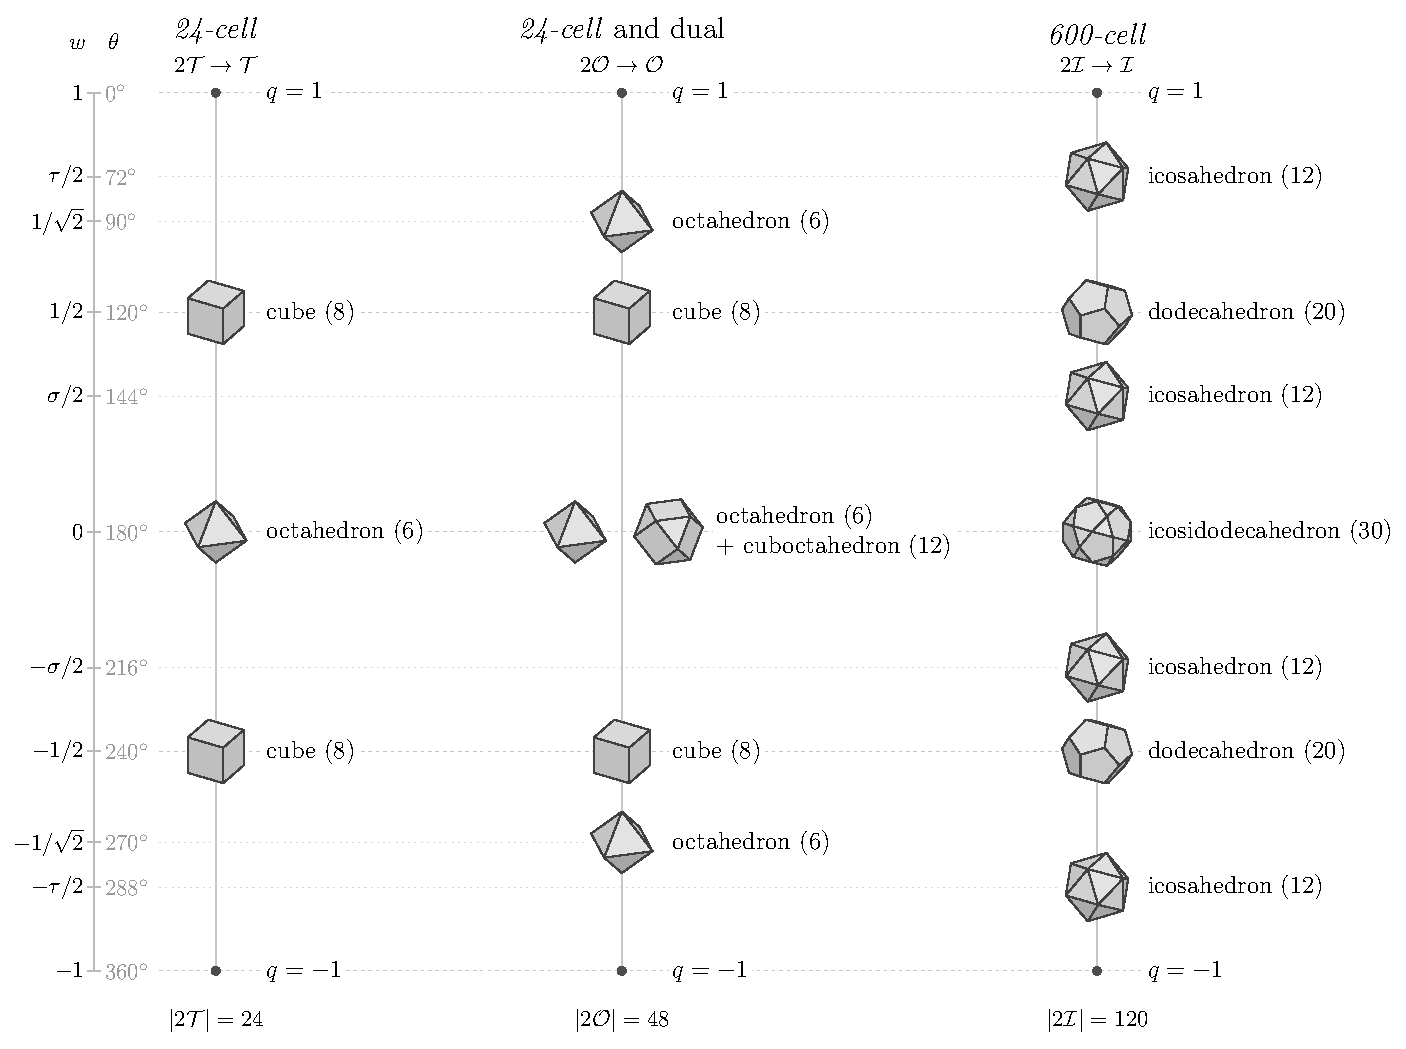
\includegraphics[width=\textwidth]{figures/section_ladder.pdf}
  \caption{The parallel sections of the three polytopes, drawn at their true latitudes. Each solid is the section at that $w$, its vertices the axes of the rotations the section holds; the count beside it is how many $\TwoG$ group elements that is, so a column sums to the order of its group. The scale on the left reads both a latitude $w$ and the turn angle $\theta = 2\arccos w$ it stands for. Below the equator, $\theta$ passes $180^\circ$, and a turn by $\theta$ about $\hat n$ is the turn by $360^\circ - \theta$ about $-\hat n$: each column is a palindrome, and the far pole is the $2\pi$ turn and not the identity. The dotted latitudes at $w = \pm 1, \pm \tfrac12, 0$ are the 24-cell's, recurring in all three columns as all three groups contain $\TwoT$. At $w = 1/2$ we see $\TwoT \subset \TwoO$ as the 24-cell's cube recurs in the $\TwoO$ column, and $\TwoT \subset \TwoI$ as five cubes are inscribed in a dodecahedron. $\TwoO$'s equator is a single section carrying two conjugacy classes, so it is drawn as its two solids. Coordinates are the Bloch axes of Section~\ref{subsec:double-cover}, computed from the group data behind Table~\ref{tab:rotation-sections}. \textcite{boolestott1900certainseriessections} developed these visualizations, and later introduced the term \textit{polytope} into English~\cite{coxeter1973regularpolytopes}. Mentally perceiving these 4D solids has also been reported, most famously of Thurston~\cite{bessis2024mathematicasecretworlda}.}
  \label{fig:section-ladder}
\end{figure}

Note the bolded row of Table~\ref{tab:rotation-sections}: the eight Paulis $\{\pm 1, \pm i, \pm j, \pm k\}$ of Section~\ref{sec:constructionrelationship} are the 24-cell's two poles and its equator, an octahedron, present in all three polytopes since all three groups contain $\TwoT$; hence two-fold edge axes for $\Tgroup$ and $\Igroup$, four-fold vertex axes for $\Ogroup$.

\chapter{Quantum Circuits for the Platonic Solid POVMs} \label{app:decker}

\textcite{decker2004quantumcircuitssinglequbit} give Naimark constructions of the five Platonic solid POVMs as projective measurements on enlarged registers. We adapt them here. In each, the solid box is Decker's circuit as published; the gate to its left on the data wire is ours---the reorientation carrying his solid into atlas orientation, written $U_R$ and derived in Section~\ref{sec:decker:using}. A prefix acts on the effects by conjugation, so each figure's $U_R$ is the \textit{inverse} of that solid's rotation $R$ in Table~\ref{tab:decker-pose}. So prefixed, each circuit measures the POVM of Appendix~\ref{sec:povm-atlas:vertices} in atlas orientation, up to the relabelling of outcomes. Section~\ref{sec:decker:using} shows that only two of the five prefixes are exact, and only over Clifford${}+T$. The optional pre-rotation $U_g$ of Section~\ref{subsec:rotated-povms} (Figure~\ref{fig:tet_povm_circuit}) is drawn dashed on each. Section~\ref{sec:decker:exactness} tackles octahedral exactness.

The construction is uniform across solids, excepting the tetrahedron, and Section~\ref{subsec:deckercircuits} states the factorization $\tilde{M}^\dagger = (A^\dagger \otimes \mathsf{F}_m^\dagger)\,Q^\dagger$ that the figures below name. One convention is fixed here: $\mathsf{F}_m = \tfrac{1}{\sqrt{m}}\bigl(\omega^{jk}\bigr)_{j,k=0}^{m-1}$ with $\omega = e^{-2\pi i/m}$, except in the cubic circuit, where we take $\omega = +i$, same as Decker. Conjugating $\mathsf{F}_m$ gives the same POVM with each orbit's outcomes reversed, so it fixes only the outcome labelling.

The data qubit $\rho$ sits on the bottom wire and ancillae $\ket{0}$ on top, matching Figure~\ref{fig:tet_povm_circuit}; all wires are measured in the computational basis. The tetrahedral and cubic registers match the vertex count $V$; the other three embed into a strictly larger register of $n$ qubits, where $2^n$ is the smallest power of two with $2^n \geq V$, so $2$, $4$, and $12$ of the basis outcomes, respectively, are by construction unreachable (zero effects).

The dodecahedron and icosahedron are dual solids sharing the symmetry group $A_5$, so their circuits share the four-stage factorization of $A^\dagger$,
\begin{equation} \label{eq:adagger}
A^\dagger \;=\; \bigl(I_2 \oplus (-\sigmaz)\bigr)\,(I_2 \otimes B)\,\mathsf{R}\,(I_2 \otimes C), \qquad \mathrm{diag}(-1, 1) = -\sigmaz,
\end{equation}
where $\mathsf{R}$ is realized as two controlled rotations on the upper ancilla; $B$ and $C$ are given with Figures~\ref{fig:dec_icos_circuit} and~\ref{fig:dec_dodec_circuit}. The unfactored $A$ is
% The prefactor here is de-symbolized on purpose --- in Appendix D the letter $c$ is the multiple of Corollary~\ref{cor:directions} and nothing else. It is printed as Decker's two factors, \sqrt{m} (his \sqrt3, \sqrt5) times his \sqrt{2/V} rescaling of the entries, not as their product 1/\sqrt2, so that his scaling is reconstructible from this paragraph alone, the cards printing nothing of A but the pointer. The display is numbered because both A_5 cards \eqref it. code/_build_povm_cards.py's check 32 pins the label, the matrix, the visible \sqrt{2/V}, the gamma/delta pairing and the pointer; its 32b parses the prefactor, the alpha/beta pair and the two pairing values back out of THIS paragraph and rebuilds Decker's circuit from them, so a drifting scale factor, radicand or pairing fails the card build --- the values may sit in a sentence, in $$ displays or in rows of this display (gathered or aligned), as `alpha^2 = X, ... beta^2 = Y,' and `gamma_icos^2 = delta_dodec^2 = X, ... delta_icos^2 = gamma_dodec^2 = Y,' with each pair on one line; reword with the builder open.
\begin{equation} \label{eq:aunfactored}
\begin{gathered} A \;=\; \sqrt{m}\,\sqrt{\tfrac{2}{V}}\begin{pmatrix}\alpha & \beta & \gamma & \delta \\ \beta & -\alpha & \delta & -\gamma \\ \gamma & -\delta & -\alpha & \beta \\ \delta & \gamma & -\beta & -\alpha\end{pmatrix}, \qquad \alpha^2 + \beta^2 = \gamma^2 + \delta^2 = 1, \\[6pt] \alpha^2 = \tfrac{1}{2} + \tfrac{1}{30}\sqrt{75 + 30\sqrt{5}}, \qquad \beta^2 = \tfrac{1}{2} - \tfrac{1}{30}\sqrt{75 + 30\sqrt{5}}, \\[2pt] \gamma_\mathrm{icos}^2 = \delta_\mathrm{dodec}^2 = \tfrac{1}{2} - \tfrac{1}{30}\sqrt{75 - 30\sqrt{5}}, \qquad \delta_\mathrm{icos}^2 = \gamma_\mathrm{dodec}^2 = \tfrac{1}{2} + \tfrac{1}{30}\sqrt{75 - 30\sqrt{5}}, \end{gathered}
\end{equation}
on the same $\alpha$ and $\beta$ for both solids, with $\gamma$ and $\delta$ swapping between the two and all four roots taken positive. The $\sqrt{2/V}$ rescales the unit pairs $(\alpha, \beta)$ and $(\gamma, \delta)$ to POVM-vector length, $\sqrt{\Tr[E_k]} = \sqrt{2/V}$; the $\sqrt{m}$, from $\mathsf{F}_3^\dagger \oplus I_1$ for the icosahedron and $\mathsf{F}_5^\dagger \oplus I_3$ for the dodecahedron, then normalizes the rows, which are orthogonal for any real entries, so $A$ is orthogonal; as $V = 4m$, the product is $1/\sqrt{2}$ for either solid.

\makeatletter\setlength\@fptop{0pt}\makeatother% top-aligns THESE five float pages only
\begin{figure}[p]
% Appendix D, Figure D.1 --- "The tetrahedral POVM, end to end".  The layout only.
%
% Layout: card_oct_body.tex's header is binding.  Deviations from it, and only
% they, are listed here.
%
%   * the sphere is Figure 1.1's own recipe_tet_sphere.pdf, reused byte for
%     byte rather than redrawn, so that Figure 1.1 and this card agree by
%     construction instead of by luck.  Assertion 21 measures whichever file
%     is named, so the reuse is checked and not exempted.
%   * the circuit is the widest of the five relative to its content
%     (336.465bp) and the side stack the tallest (four atoms: $U_A$, $\alpha$,
%     $\beta$, and $S$ with $H$), so band 2 runs 344pt + 103pt.
%   * BAND 4 HAS NO RAY LIST.  These four vertices form no antipodal pair, so
%     there is no coin: head 4 reads "No coin over axes" and the band is one
%     label.  Its first sentence is the only place on the five cards where
%     the two randomized protocols meet, and they must meet as a contrast --
%     without it a reader concludes this solid admits no randomization at
%     all, which its own dashed $U_g$ contradicts one band above.  Its
%     second sentence is the one claim on the five pages that bsc-thesis.tex
%     makes nowhere else: draw 2T against an aligned vertex anyway and the
%     readout's two poles assemble the CUBE, eight effects of weight 2/8.
%     Not a failure -- a different POVM, and the only Platonic case where
%     the vertex orbit is not already antipodally closed.  It is also this
%     card's one outward pointer, to Figure D.3.  Head 4 carries no Appendix
%     A pointer: there are no coin words to route.
%   * the reserve is 171.63pt, the largest of the five by a wide margin, and it sits
%     below the caption as trailing white.  The tetrahedron IS the small card
%     -- four vertices, two wires, no dead outcome, no coin -- and Figure 1.1
%     already carries it in full.
% All macros below are \def and therefore local to the figure environment.
\parindent=0pt \parskip=0pt
% Auto-generated by code/_build_povm_cards.py -- DO NOT EDIT.
% The data blocks of the tetrahedral card of Appendix D
% (paper/figures/card_tet_body.tex \input's this and calls them).  Every
% number is derived from code/data/*.npz, Decker's circuits as
% randomized_decker rebuilds them, Figure 1.1's own \RecipeSeriesStrip, and
% Tables E.1, 5.2, D.1, D.3 and D.4, and is checked back against them before
% this file is written; see the builder's docstring for the checks (and
% _povm_cards_controls.py, which shows each of them failing on one corrupted
% literal: 100 negative controls, all aborting, 0 stale).
% Requires: booktabs, mathtools, hyperref, and the thesis macros \Id, \pmat,
% \bra, \ket, \braket, \Tr, \C, \sigmavec, \TwoT, \TwoO, \TwoI, \phig,
% \invphig, \sigmaz.  The body defines \NIS, \CTR, \PBOX, \COL, \FULLHEAD,
% \BANDRULE and \TAB, which \CardSide and the tables use.
% Regenerate with `cd code && uv run _build_povm_cards.py`.

\newcommand{\CTitle}{The tetrahedral POVM, end to end}
\newcommand{\CPtrStrip}{Introduction reference: Figure~\ref{fig:tetrahedron-recipe}}
\newcommand{\CHeadA}{Vertices and effects, $E_k = \tfrac1V(\Id + \hat n_k \cdot \sigmavec)$.}
\newcommand{\CPtrA}{Table~\ref{tab:povm-atlas} $\cdot$ Equation~\eqref{eq:povmform}}
\newcommand{\CHeadB}{Circuit; the dashed $U_g$ is an optional prepended rotation.}
\newcommand{\CPtrB}{Section~\ref{subsec:rotated-povms} $\cdot$ Table~\ref{tab:decker-pose}}
\newcommand{\CHeadC}{Register $\to$ vertex, top wire first}
\newcommand{\CPtrC}{Table~\ref{tab:decker-labels} $\cdot$ Section~\ref{sec:decker:using}}
\newcommand{\CHeadD}{No coin over axes}
\newcommand{\CPtrD}{Table~\ref{tab:decker-vs-coin} $\cdot$ Section~\ref{subsec:randomized-implementations}}

\newcommand{\CStrip}{{\footnotesize\setlength{\tabcolsep}{4pt}\renewcommand{\arraystretch}{0.88}%
\begin{tabular}{@{}c c c c l l l@{}}
\toprule
$V$ & group & anc. & dead & reorientation exact? & relabelling & \hyperref[tab:decker-vs-coin]{coin over axes}\\
\midrule
4 & $\TwoT$ & 1 & 0 & $T^\dagger$, over Clifford${}+T$ & identity & none: no antipodes\\
\midrule
\multicolumn{7}{@{}l@{}}{only the octahedral coin is exact --- this dilation is not (Theorem~\ref{thm:main}, Appendix~\ref{sec:decker:exactness})}\\
\bottomrule
\end{tabular}}}

\newcommand{\CardVertexTable}{%
\begin{tabular}{@{}r l c r@{}}
\toprule
$k$ & $\hat n_k$\ $(\times\tfrac{1}{\sqrt3})$ & $E_k\ (\times\tfrac{\sqrt3}{12})$ & $\bra{0}E_k\ket{0}$ \\
\midrule
$1$ & $(+1,\,+1,\,+1)$ & $\pmat{\sqrt3+1 & 1-i \\ 1+i & \sqrt3-1}$ & $0.3943$ \\ \addlinespace[3pt]
$2$ & $(-1,\,-1,\,+1)$ & $\pmat{\sqrt3+1 & -1+i \\ -1-i & \sqrt3-1}$ & $0.3943$ \\ \addlinespace[3pt]
$3$ & $(-1,\,+1,\,-1)$ & $\pmat{\sqrt3-1 & -1-i \\ -1+i & \sqrt3+1}$ & $0.1057$ \\ \addlinespace[3pt]
$4$ & $(+1,\,-1,\,-1)$ & $\pmat{\sqrt3-1 & 1+i \\ 1-i & \sqrt3+1}$ & $0.1057$ \\ \addlinespace[3pt]
\bottomrule
\end{tabular}
}

\newcommand{\CIdent}{$\sum_k E_k = \Id$, $\Tr E_k = \tfrac12$, rank one, a $2$-design; $|\braket{\psi_j}{\psi_k}|^2 = \tfrac13$ for $j \neq k$: the SIC condition.}
\newcommand{\CIdentB}{}

\newcommand{\CParams}{$U_R$ inverts Table~\ref{tab:decker-pose}'s $R$; a drawn $U_g$ twirls and relabels outcomes by $g^{-1}$.\par\vskip1pt $Q^\dagger$: the CNOT $\ket{00}\mapsto\ket{00}$, $\ket{11}\mapsto\ket{01}$; the ancilla-controlled $S$ realizes $\mathrm{diag}(1,1,1,i)$\par\vskip1pt $\tilde{M}^\dagger = (I_2 \otimes \mathsf{F}_2)\,\mathrm{diag}(1,1,1,i)\,(U_A \otimes I_2)\,Q^\dagger$, the Naimark extension unitary the solid box implements}

\newcommand{\CardSide}{\CTR{\hsize}{$U_A = \sqrt2\,\pmat{\alpha & \beta \\ \beta & -\alpha}$}\NIS{4pt}\CTR{\hsize}{$\alpha = \sqrt{(3+\sqrt3)/12}$}\NIS{4pt}\CTR{\hsize}{$\beta = \sqrt{(3-\sqrt3)/12}$}\NIS{4pt}\CTR{\hsize}{$S = \mathrm{diag}(1,i)$, $H = \mathsf{F}_2$}}

\newcommand{\CardKey}{%
\begin{tabular}{@{}c c c@{}}
\toprule
& \multicolumn{2}{c}{\footnotesize lower} \\
{\footnotesize upper} & $\mathtt{0}$ & $\mathtt{1}$ \\
\midrule
$\mathtt{0}$ & 1 & 2 \\
$\mathtt{1}$ & 3 & 4 \\
\bottomrule
\end{tabular}
}

\newcommand{\CKappa}{Run $U_R$ and read the key, or skip $U_R$ and read Decker's own numbered list~\cite{decker2004quantumcircuitssinglequbit}: either way $\kappa = 1$, free. His circuit with our list, index for index, is the mismatch: $\kappa = +0.804738$; under the drawn twirl it costs a $1/\kappa^2 = 1.54\times$ premium in shots, never a bias.}

\newcommand{\CRays}{}

\newcommand{\CCoin}{The dilation is forced; a drawn $U_g$ still twirls it. Align a vertex and draw from $\TwoT$ anyway: each readout reports an axis, not a vertex, and the eight effects assembled are the cube's (Figure~\ref{fig:dec_cube_circuit}).}

\long\def\NIS#1{\vskip #1\nointerlineskip}
\long\def\CTR#1#2{\hbox to #1{\hss #2\hss}}
\long\def\PBOX#1#2{\vtop{\hsize=#1\parindent0pt\sloppy\emergencystretch=1.5em\small #2}}
\long\def\COL#1#2{\vtop{\hsize=#1\parindent0pt\hbox{}\nointerlineskip #2}}
\long\def\FULLHEAD#1#2#3{\hbox to \hsize{\small\textbf{#1}\,#2\hfil{\footnotesize #3}}}
\def\BANDRULE{\vskip2pt\hrule height0.5pt\vskip1.5pt\nointerlineskip}
\long\def\TAB#1{{\small\renewcommand{\arraystretch}{0.88}\setlength{\tabcolsep}{3pt}#1}}
%
\vbox{\hsize\textwidth\parindent0pt
%
% --- title and the header strip: Figure 1.1's own row -----------------------
\hbox to \hsize{\large\bfseries \CTitle\hfil{\normalfont\footnotesize \CPtrStrip}}%
\NIS{5pt}%
\hbox{\CStrip}%
\BANDRULE
%
% --- band 1: the object -----------------------------------------------------
\FULLHEAD{1}{\CHeadA}{\CPtrA}%
\NIS{5pt}%
\hbox to \hsize{%
  \COL{170pt}{\CTR{170pt}{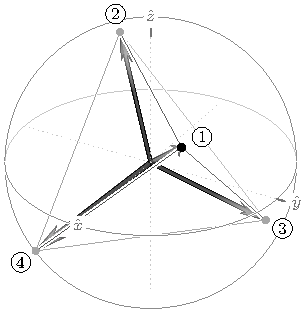
\includegraphics{figures/recipe_tet_sphere.pdf}}}%
  \hfil
  \COL{277pt}{\hbox to 277pt{\hfil\TAB{\CardVertexTable}}}%
}%
\NIS{4pt}%
\PBOX{\hsize}{\CIdent}%
\BANDRULE
%
% --- band 2: the machine ----------------------------------------------------
\FULLHEAD{2}{\CHeadB}{\CPtrB}%
\NIS{5pt}%
\hbox to \hsize{%
  \COL{344pt}{\hbox to 344pt{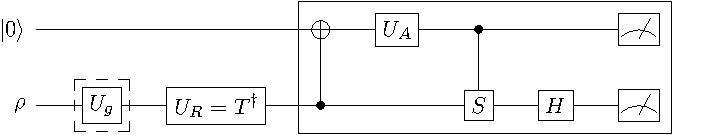
\includegraphics{figures/card_dec_tet.pdf}\hss}}%
  \hfil
  \COL{103pt}{\small\CardSide}%
}%
\NIS{5pt}%
\PBOX{\hsize}{\CParams}%
\BANDRULE
%
% --- band 3: the readout ----------------------------------------------------
\FULLHEAD{3}{\CHeadC}{\CPtrC}%
\NIS{5pt}%
\hbox to \hsize{%
  \COL{120pt}{\TAB{\CardKey}}%
  \hfil
  \COL{324pt}{\PBOX{324pt}{\CKappa}}%
}%
\BANDRULE
%
% --- band 4: the alternative ------------------------------------------------
\FULLHEAD{4}{\CHeadD}{\CPtrD}%
\NIS{5pt}%
\PBOX{\hsize}{\CCoin}%
}%

\caption{The solid box is \textcite[Fig.~7]{decker2004quantumcircuitssinglequbit}'s; $U_R$ and $U_g$ are ours.}
\label{fig:dec_tet_circuit}
\end{figure}

\begin{figure}[p]
% Appendix D, Figure D.2 --- "The octahedral POVM, end to end".  The layout only.
%
% THIS FILE IS THE TEMPLATE.  The other four card bodies declare this header
% binding and list only their own deviations.  Every rule below was bought with
% a measurement in the real class (11pt scrbook, a4paper, margin=1in,
% \textwidth 452.9679pt, \textheight 700.50687pt); do not "tidy" any of them.
%
% WHAT A CARD IS.  The card labels rather than narrates: a header strip the
% reader has already met in Figure 1.1, four objects, one label per object,
% and a pointer per band.  The strip is Figure 1.1's own \RecipeSeriesStrip --
% its column heads and this solid's row, character for character, minus the
% name column -- plus one spanned footer carrying the thesis's exactness
% conjunction in nine words.  That is what makes the recognition a build
% check (assertion 30) rather than a hope.
%
% Everything numeric comes from ../code/data/card_oct_data.tex, which
% code/_build_povm_cards.py writes after its checks against the npz data,
% Decker's circuits as randomized_decker rebuilds them, Figure 1.1's own
% recipe_tet_data.tex, and Tables E.1, 5.2, D.1, D.3 and D.4 -- and refuses to
% write a byte if any of them fails.  The heads, the labels and the caption are
% emitted too, so this file holds the LAYOUT and nothing else; assertion 12
% requires the facts on the page verbatim and assertion 29 parses the printed
% surface back out of the data file, cell by cell.
%
% The four numerals must read 1..4 straight down the left edge.
%
% ASSEMBLY RULES (each one bought with a measurement; do not "tidy" them):
%   * rows are stacked in one \vbox and separated by \vskip<n>pt\nointerlineskip,
%     and EVERY source line inside the \vbox ends in %.  Without either, LaTeX
%     adds ~13.6pt of baseline glue PER ROW: the same dodecahedron body measured
%     726.79pt with the glue and 662.96pt without.
%   * the body is a plain \vbox, NEVER \vbox to.  Equal-height bodies were
%     measured and rejected: they strand the tetrahedron's caption 152pt below
%     its own content.  The five start at the same height because the float
%     pages are top-aligned locally (bsc-thesis.tex brackets these five floats
%     with \@fptop 0pt and restores the default after the \clearpage); ragged
%     bottoms, aligned tops.
%   * a two-column row is one \hbox to \hsize{<left>\hfil<right>} whose columns
%     are \vtop's opening with \hbox{}\nointerlineskip, which is what top-aligns
%     them (a \vtop otherwise aligns on its first line's baseline).
%   * every prose block is \PBOX: \sloppy plus \emergencystretch, or the
%     unbreakable math atoms throw overfull boxes into the neighbouring column.
%     WIDEN A COLUMN BY 4pt BEFORE TOUCHING A SENTENCE.
%   * NOTHING may be glued to the right of the U_R atom.  At \footnotesize this
%     card's product measured 181.64pt bare and 190.89pt with an em-dash
%     attached, a 3.58pt overfull box.  Every rider therefore follows the
%     CLAUSE, never the formula, and the generator's params() carries the note.
%   * the parameter block is ONE FORMULA PER LINE (\par\vskip1pt between), full
%     width, at \small.  Set as a justified paragraph at \footnotesize, the
%     inline 4x4 A opens a four-line hole; A belongs to the chapter head
%     (assertion 32) and the block reads as a list.  Justified, not
%     \raggedright: \raggedright costs +12.69pt.
%   * the vertex table and the key are set flush RIGHT in their columns; the
%     circuit is set flush LEFT, never centred, because all 13.73bp of xy-pic's
%     slack is on the right and centring hangs the \lstick ket bar into the
%     left margin.
%   * FOUR band rules, one per band, \vskip2pt\hrule height0.5pt\vskip1.5pt =
%     4.00pt each.  No other rules, no boxes, no tints, NO COLOUR: the
%     numbered chips do identity, so the pages are greyscale-safe.
%   * every head must fit on ONE line with its pointer.  Measured natural
%     widths against the 452.9679pt line: head 2 with its pointers is 348.82
%     on all five, and head 4 is the tightest at 437.53 on the A_5 pair
%     (", rightmost factor first" + three pointers, 15.44pt of slack).
%     Re-measure before rewording any head or giving a band a fourth pointer;
%     the strip and the dodecahedron's ray list may not change without
%     re-measuring either (the ray list is 443.86pt natural -- 9.11pt of
%     slack).
%   * \PanelScale 2.47 on all five, Figure 1.1's own.  The tetrahedron reuses
%     Figure 1.1's recipe_tet_sphere.pdf byte for byte, not redrawn.
%   * the float, not the body, is what LaTeX measures: \@largefloatcheck
%     compares \ht\@currbox against \textheight = 700.50687pt.  Measure over
%     the FLOAT: a pass over the body alone leaves the kappa label's \cite
%     unresolved -- no biber -- and inflates.  Measured that way, with
%     bsc-thesis.aux's labels replayed and biber run, the five reserves are
%     tet 171.63pt, oct 90.35, cube 35.99, icos 56.01, dodec 21.30; a card
%     that takes an extra band-4 line pays about 11pt of its reserve for it.
%   * the caption is ONE line on all five and must stay one: a second line
%     costs 13.60pt against the dodecahedron's 21.30pt of reserve.  Measured
%     with \@makecaption in this class: the shipped caption sets 429.82pt
%     (Fig.~7) / 435.29pt (Figs.~11 and~13) WITH its "Figure D.5.: " label,
%     against the 452.9679pt line, and the caption box is 23.60pt with 0
%     overfull.  A longer wording that also calls the $U_g$ box dashed
%     ("$U_R$ and the dashed $U_g$ are ours") measures
%     485.24 / 490.71pt and does NOT break: \@makecaption still returns a
%     23.60pt box and TeX reports Overfull \hbox 9.07 / 14.55pt.  Head 2
%     names the dashed box one band above, which is what pays for the cut.
%   * THE DODECAHEDRON IS THE BINDING CARD, at 21.30pt of reserve.  Every
%     literal in the generator's emitters is shared, so any wording change
%     must be re-measured against card_dodec_body.tex before it ships.  Two
%     of its objects are already at the edge: the kappa label (its box must
%     stay near the 75.56pt key) and the U_R parameter line (one word of
%     rider wraps it: "twirls the noise" measures 490.81pt against the
%     452.9679pt line; "twirls" ships at 448.53).  Its ray line is 443.86pt
%     natural -- 9.11pt of slack.
%   * ... but one shared literal binds its WIDTH elsewhere: the
%     M-tilde-dagger line's gloss, ", the Naimark extension unitary the solid
%     box implements".  The tetrahedron prints the longest of the five
%     formulas, so the gloss sets 438.23pt there against 351.56 on the
%     dodecahedron -- 14.73pt of slack, and "the boxed circuit" in place of
%     "the solid box" misses by 3.02pt and wraps.
%
% WORDING RULES:
%   * print the positive with the negative.  The strip's spanned footer carries
%     the conjunction on every card -- "only the octahedral coin is exact ---
%     this dilation is not" -- with the negative also in the `reorientation
%     exact?` cell beside it; on this card the positive is its own row's
%     `3 axes --- exact`.  The dilation clause is what binds Theorem 1 to the
%     circuit printed 10cm below it and may not be compressed away.  Its
%     polarity is fragile: "exact, this dilation included" reads as putting
%     the dilation AMONG the exact things -- the appositive needs the host
%     Figure 1.1 gives it ("any dilation, this one included") -- so this card
%     spells the negative out instead.
%   * Decker is named WITH the cite wherever his objects appear: the caption
%     (the solid box) and the kappa label (his own outcome list).  Figure 1.1
%     prints no cold names; the cards do the opposite -- a \cite for
%     everything belonging to Decker, and his name with it.
%   * say what a reorientation IS before asking whether it is exact -- the
%     chapter head does it one page earlier, in its second sentence, and the
%     strip's head is Figure 1.1's own `reorientation exact?`.
%   * the two randomized protocols stay distinct.  "coin over axes" is
%     Figure 1.1's hyperlinked phrase, in the strip and in head 4; the twirl
%     appears as "a drawn $U_g$ twirls and relabels outcomes by $g^{-1}$" on
%     the parameter line, as "the drawn twirl" in the kappa label, and on the
%     tetrahedron as the contrast in band 4.  Every card's protocol line
%     closes with its own DRAW NOTE, the five together a ladder: no
%     projective route at all (the tetrahedron, where drawing anyway
%     assembles the cube), the twirl binding on this card and the cube
%     (realization needs only the three or four words printed above the
%     sentence), the two meeting at the icosahedron (the two-jobs sentence,
%     still that card's alone), realization binding on the dodecahedron.
%     Check 19d derives all five and pins each phrase to its own card: the
%     two-jobs one here would contradict the thesis's own counterexample,
%     this card's coin realizing and twirling nothing.  Head 4's "no ancilla"
%     is what says the coin REPLACES the dilation rather than running inside
%     it -- neither Figure 1.1 (which never explains the coin) nor the
%     protocol line supplies that, and it negates the strip's own `anc.` cell
%     two bands above, so it costs no new noun.
%   * direction is g^{-1}.  Never "acts on" -- assertion 11 greps this file.
%   * no italic run-in heads.
%   * the register convention lives ON THE OBJECT: the key rectangle's `upper`
%     stub and `lower` spanned head, whose bit widths say which wires those
%     are, plus head 3's "top wire first".
%   * one page, two F's: the circuit's upright sans $\mathsf F_3^\dagger$ and
%     band 4's bold $\mathbf F$ are different objects a band apart.  Never
%     gloss $\mathbf F = \mathbf H\mathbf S^\dagger$ here.
%   * the coin's order is the drawn word FIRST, the fixed alignment after it,
%     and the alignment is a LABEL, not a sentence ("($\Id$ here)").  Assertion
%     19b builds the reversed order and requires it to miss the vertex set.
%
% All macros below are \def and therefore local to the figure environment.
\parindent=0pt \parskip=0pt
% Auto-generated by code/_build_povm_cards.py -- DO NOT EDIT.
% The data blocks of the octahedral card of Appendix D
% (paper/figures/card_oct_body.tex \input's this and calls them).  Every
% number is derived from code/data/*.npz, Decker's circuits as
% randomized_decker rebuilds them, Figure 1.1's own \RecipeSeriesStrip, and
% Tables E.1, 5.2, D.1, D.3 and D.4, and is checked back against them before
% this file is written; see the builder's docstring for the checks (and
% _povm_cards_controls.py, which shows each of them failing on one corrupted
% literal: 100 negative controls, all aborting, 0 stale).
% Requires: booktabs, mathtools, hyperref, and the thesis macros \Id, \pmat,
% \bra, \ket, \braket, \Tr, \C, \sigmavec, \TwoT, \TwoO, \TwoI, \phig,
% \invphig, \sigmaz.  The body defines \NIS, \CTR, \PBOX, \COL, \FULLHEAD,
% \BANDRULE and \TAB, which \CardSide and the tables use.
% Regenerate with `cd code && uv run _build_povm_cards.py`.

\newcommand{\CTitle}{The octahedral POVM, end to end}
\newcommand{\CPtrStrip}{Introduction reference: Figure~\ref{fig:tetrahedron-recipe}}
\newcommand{\CHeadA}{Vertices and effects, $E_k = \tfrac1V(\Id + \hat n_k \cdot \sigmavec)$.}
\newcommand{\CPtrA}{Table~\ref{tab:povm-atlas} $\cdot$ Equation~\eqref{eq:povmform}}
\newcommand{\CHeadB}{Circuit; the dashed $U_g$ is an optional prepended rotation.}
\newcommand{\CPtrB}{Section~\ref{subsec:rotated-povms} $\cdot$ Table~\ref{tab:decker-pose}}
\newcommand{\CHeadC}{Register $\to$ vertex, top wire first; --- never fires}
\newcommand{\CPtrC}{Table~\ref{tab:decker-labels} $\cdot$ Section~\ref{sec:decker:using}}
\newcommand{\CHeadD}{Coin over axes, no ancilla, $\ket0$-vertex first}
\newcommand{\CPtrD}{Table~\ref{tab:decker-vs-coin} $\cdot$ Section~\ref{subsec:randomized-implementations} $\cdot$ Table~\ref{tab:binary-octahedral-group-2o}}

\newcommand{\CStrip}{{\footnotesize\setlength{\tabcolsep}{4pt}\renewcommand{\arraystretch}{0.88}%
\begin{tabular}{@{}c c c c l l l@{}}
\toprule
$V$ & group & anc. & dead & reorientation exact? & relabelling & \hyperref[tab:decker-vs-coin]{coin over axes}\\
\midrule
6 & $\TwoO$ & 2 & 2 & no thesis gate set & permuted & 3 axes --- \textbf{exact}\\
\midrule
\multicolumn{7}{@{}l@{}}{only the octahedral coin is exact --- this dilation is not (Theorem~\ref{thm:main}, Appendix~\ref{sec:decker:exactness})}\\
\bottomrule
\end{tabular}}}

\newcommand{\CardVertexTable}{%
\begin{tabular}{@{}r l c r@{}}
\toprule
$k$ & $\hat n_k$ & $E_k\ (\times\tfrac16)$ & $\bra{0}E_k\ket{0}$ \\
\midrule
$1$ & $(+1,\,\phantom{+}0,\,\phantom{+}0)$ & $\pmat{1 & 1 \\ 1 & 1}$ & $0.1667$ \\ \addlinespace[3pt]
$2$ & $(-1,\,\phantom{+}0,\,\phantom{+}0)$ & $\pmat{1 & -1 \\ -1 & 1}$ & $0.1667$ \\ \addlinespace[3pt]
$3$ & $(\phantom{+}0,\,+1,\,\phantom{+}0)$ & $\pmat{1 & -i \\ i & 1}$ & $0.1667$ \\ \addlinespace[3pt]
$4$ & $(\phantom{+}0,\,-1,\,\phantom{+}0)$ & $\pmat{1 & i \\ -i & 1}$ & $0.1667$ \\ \addlinespace[3pt]
$5$ & $(\phantom{+}0,\,\phantom{+}0,\,+1)$ & $\pmat{2 & 0 \\ 0 & 0}$ & $0.3333$ \\ \addlinespace[3pt]
$6$ & $(\phantom{+}0,\,\phantom{+}0,\,-1)$ & $\pmat{0 & 0 \\ 0 & 2}$ & $0.0000$ \\ \addlinespace[3pt]
\bottomrule
\end{tabular}
}

\newcommand{\CIdent}{$\sum_k E_k = \Id$, $\Tr E_k = \tfrac13$, rank one, a $3$-design; the Pauli eigenprojectors, $\times\tfrac13$.}
\newcommand{\CIdentB}{}

\newcommand{\CParams}{$U_R = R_{\hat z}(180^\circ)R_{\hat y}(-\arccos(1/\sqrt3))R_{\hat z}(-45^\circ)$, rightmost factor first, inverts Table~\ref{tab:decker-pose}'s $R$; a drawn $U_g$ twirls and relabels outcomes by $g^{-1}$.\par\vskip1pt $Q_8^\dagger$: the CNOT $\ket{000}\mapsto\ket{000}$, $\ket{101}\mapsto\ket{001}$; $\mathsf{F}_3^\dagger \oplus I_1 \in \C^{4\times4}$, lower two wires\par\vskip1pt $\tilde{M}^\dagger_8 = (U_A \otimes (\mathsf{F}_3^\dagger \oplus I_1))\,Q_8^\dagger$, the Naimark extension unitary the solid box implements}

\newcommand{\CardSide}{\CTR{\hsize}{$U_A = \sqrt3\,\pmat{\alpha & \beta \\ \beta & -\alpha}$}\NIS{4pt}\CTR{\hsize}{$\alpha = \sqrt{(3+\sqrt3)/18}$}\NIS{4pt}\CTR{\hsize}{$\beta = \sqrt{(3-\sqrt3)/18}$}}

\newcommand{\CardKey}{%
\begin{tabular}{@{}c c c c c@{}}
\toprule
& \multicolumn{4}{c}{\footnotesize lower} \\
{\footnotesize upper} & $\mathtt{00}$ & $\mathtt{01}$ & $\mathtt{10}$ & $\mathtt{11}$ \\
\midrule
$\mathtt{0}$ & 5 & 3 & 1 & --- \\
$\mathtt{1}$ & 6 & 4 & 2 & --- \\
\bottomrule
\end{tabular}
}

\newcommand{\CKappa}{Run $U_R$ and read the key, or skip $U_R$ and read Decker's own numbered list~\cite{decker2004quantumcircuitssinglequbit}: either way $\kappa = 1$, free. His circuit with our list, index for index, is the mismatch: $\kappa = +0.321975$; under the drawn twirl it costs a $1/\kappa^2 = 9.65\times$ premium in shots, never a bias.}

\newcommand{\CRays}{$\mathbf{F}^\dagger$~$1$,\,$2$ $\cdot$ $\mathbf{F}$~$3$,\,$4$ $\cdot$ $\Id$~$5$,\,$6$}

\newcommand{\CCoin}{Draw one, apply it, then the alignment ($\Id$ here); measure $Z$. Random Pauli measurement. Realization needs only these three; among groups it is the twirl that forces the full $\TwoT$ draw (Section~\ref{sec:shadows:bills}).}

\long\def\NIS#1{\vskip #1\nointerlineskip}
\long\def\CTR#1#2{\hbox to #1{\hss #2\hss}}
\long\def\PBOX#1#2{\vtop{\hsize=#1\parindent0pt\sloppy\emergencystretch=1.5em\small #2}}
\long\def\COL#1#2{\vtop{\hsize=#1\parindent0pt\hbox{}\nointerlineskip #2}}
\long\def\FULLHEAD#1#2#3{\hbox to \hsize{\small\textbf{#1}\,#2\hfil{\footnotesize #3}}}
\def\BANDRULE{\vskip2pt\hrule height0.5pt\vskip1.5pt\nointerlineskip}
\long\def\TAB#1{{\small\renewcommand{\arraystretch}{0.88}\setlength{\tabcolsep}{3pt}#1}}
%
\vbox{\hsize\textwidth\parindent0pt
%
% --- title and the header strip: Figure 1.1's own row -----------------------
\hbox to \hsize{\large\bfseries \CTitle\hfil{\normalfont\footnotesize \CPtrStrip}}%
\NIS{5pt}%
\hbox{\CStrip}%
\BANDRULE
%
% --- band 1: the object -----------------------------------------------------
% Where the effect table is the taller column, the sphere is vertically
% centred against it.  The offset is computed at TeX time from the two
% boxes, so a regenerated table cannot strand a hand-measured constant;
% the row's total height is unchanged (the taller column still sets it).
% The other three cards keep the template's top alignment -- their panels
% are the taller column.
\FULLHEAD{1}{\CHeadA}{\CPtrA}%
\NIS{5pt}%
\setbox0=\hbox{\TAB{\CardVertexTable}}%
\setbox2=\hbox{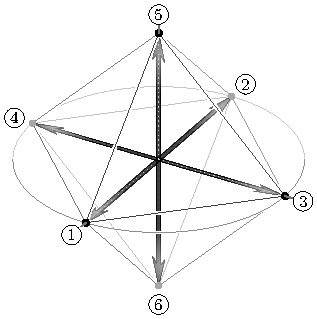
\includegraphics{figures/card_oct_sphere.pdf}}%
\dimen0=\dimexpr(\ht0+\dp0-\ht2-\dp2)/2\relax
\hbox to \hsize{%
  \COL{170pt}{\vskip\dimen0 \CTR{170pt}{\box2}}%
  \hfil
  \COL{277pt}{\hbox to 277pt{\hfil\box0}}%
}%
\NIS{4pt}%
\PBOX{\hsize}{\CIdent}%
\BANDRULE
%
% --- band 2: the machine ----------------------------------------------------
\FULLHEAD{2}{\CHeadB}{\CPtrB}%
\NIS{5pt}%
\hbox to \hsize{%
  \COL{264pt}{\hbox to 264pt{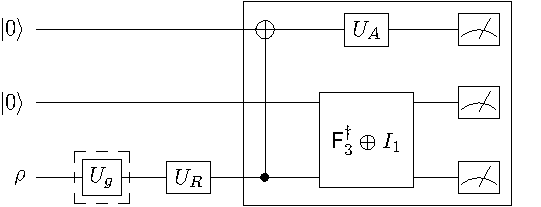
\includegraphics{figures/card_dec_oct.pdf}\hss}}%
  \hfil
  \COL{183pt}{\small\CardSide}%
}%
\NIS{5pt}%
\PBOX{\hsize}{\CParams}%
\BANDRULE
%
% --- band 3: the readout ----------------------------------------------------
\FULLHEAD{3}{\CHeadC}{\CPtrC}%
\NIS{5pt}%
\hbox to \hsize{%
  \COL{150pt}{\TAB{\CardKey}}%
  \hfil
  \COL{294pt}{\PBOX{294pt}{\CKappa}}%
}%
\BANDRULE
%
% --- band 4: the alternative ------------------------------------------------
\FULLHEAD{4}{\CHeadD}{\CPtrD}%
\NIS{5pt}%
\PBOX{\hsize}{\CRays}%
\NIS{2pt}%
\PBOX{\hsize}{\CCoin}%
}%

\caption{The solid box is \textcite[Fig.~11]{decker2004quantumcircuitssinglequbit}'s; $U_R$ and $U_g$ are ours.}
\label{fig:dec_oct_circuit}
\end{figure}

\begin{figure}[p]
% Appendix D, Figure D.3 --- "The cubic POVM, end to end".  The layout only.
%
% Layout: card_oct_body.tex's header is binding.  Deviations from it, and only
% they, are listed here.
%
%   * the sphere column is 162pt and the table column 285pt: eight rows with
%     an effect column is the widest vertex table of the five.
%   * the key is the widest of the five (190pt): eight live cells in a
%     2 x 4 rectangle with no dead column.
%   * $\omega = +i$ is deliberately NOT printed: the chapter head states the
%     cubic circuit's Fourier convention one page earlier, and the caption
%     this card replaces never printed it either.
% All macros below are \def and therefore local to the figure environment.
\parindent=0pt \parskip=0pt
\input{../code/data/card_cube_data}
\long\def\NIS#1{\vskip #1\nointerlineskip}
\long\def\CTR#1#2{\hbox to #1{\hss #2\hss}}
\long\def\PBOX#1#2{\vtop{\hsize=#1\parindent0pt\sloppy\emergencystretch=1.5em\small #2}}
\long\def\COL#1#2{\vtop{\hsize=#1\parindent0pt\hbox{}\nointerlineskip #2}}
\long\def\FULLHEAD#1#2#3{\hbox to \hsize{\small\textbf{#1}\,#2\hfil{\footnotesize #3}}}
\def\BANDRULE{\vskip2pt\hrule height0.5pt\vskip1.5pt\nointerlineskip}
\long\def\TAB#1{{\small\renewcommand{\arraystretch}{0.88}\setlength{\tabcolsep}{3pt}#1}}
%
\vbox{\hsize\textwidth\parindent0pt
%
% --- title and the header strip: Figure 1.1's own row -----------------------
\hbox to \hsize{\large\bfseries \CTitle\hfil{\normalfont\footnotesize \CPtrStrip}}%
\NIS{5pt}%
\hbox{\CStrip}%
\BANDRULE
%
% --- band 1: the object -----------------------------------------------------
% The sphere is vertically centred against the taller eight-row effect
% table, by TeX-time arithmetic as on the octahedron card; the row's
% height is unchanged.
\FULLHEAD{1}{\CHeadA}{\CPtrA}%
\NIS{5pt}%
\setbox0=\hbox{\TAB{\CardVertexTable}}%
\setbox2=\hbox{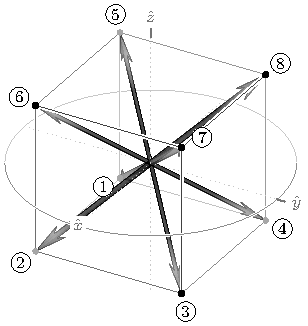
\includegraphics{figures/card_cube_sphere.pdf}}%
\dimen0=\dimexpr(\ht0+\dp0-\ht2-\dp2)/2\relax
\hbox to \hsize{%
  \COL{162pt}{\vskip\dimen0 \CTR{162pt}{\box2}}%
  \hfil
  \COL{285pt}{\hbox to 285pt{\hfil\box0}}%
}%
\NIS{4pt}%
\PBOX{\hsize}{\CIdent}%
\BANDRULE
%
% --- band 2: the machine ----------------------------------------------------
\FULLHEAD{2}{\CHeadB}{\CPtrB}%
\NIS{5pt}%
\hbox to \hsize{%
  \COL{268pt}{\hbox to 268pt{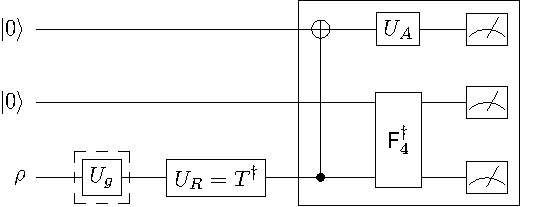
\includegraphics{figures/card_dec_cube.pdf}\hss}}%
  \hfil
  \COL{179pt}{\small\CardSide}%
}%
\NIS{5pt}%
\PBOX{\hsize}{\CParams}%
\BANDRULE
%
% --- band 3: the readout ----------------------------------------------------
\FULLHEAD{3}{\CHeadC}{\CPtrC}%
\NIS{5pt}%
\hbox to \hsize{%
  \COL{190pt}{\TAB{\CardKey}}%
  \hfil
  \COL{254pt}{\PBOX{254pt}{\CKappa}}%
}%
\BANDRULE
%
% --- band 4: the alternative ------------------------------------------------
\FULLHEAD{4}{\CHeadD}{\CPtrD}%
\NIS{5pt}%
\PBOX{\hsize}{\CRays}%
\NIS{2pt}%
\PBOX{\hsize}{\CCoin}%
}%

\caption{The solid box is \textcite[Fig.~9]{decker2004quantumcircuitssinglequbit}'s; $U_R$ and $U_g$ are ours.}
\label{fig:dec_cube_circuit}
\end{figure}

\begin{figure}[p]
% Appendix D, Figure D.4 --- "The icosahedral POVM, end to end".  The layout only.
%
% Layout: card_oct_body.tex's header is binding.  Deviations from it, and only
% they, are listed here.
%
%   * band 1 NESTS the worked $E_1$ under the two vertex blocks, in the slack
%     the sphere leaves beside them -- zero words, and it is what gives the
%     covariance rule $E_{g(k)} = U_g E_k U_g^\dagger$ an effect to act on.
%     It costs 0pt: the panel, not the right column, sets the row.
%   * the vertex blocks carry no effect column (twelve two-line pmatrices do
%     not fit beside a panel), which is why the worked effect is printed.
%   * band 2 runs 377pt + 75pt: the circuit is 375.032bp and the side column
%     holds $B$ and $C$ -- the two matrices that DIFFER between this card and
%     the dodecahedron's.  The unfactored $A$, which the pair shares, is the
%     chapter head's (assertion 32 refuses to write this card until it is
%     there).  Measured: A on the card costs 43.81pt.
%   * head 4 carries ", rightmost factor first": this card prints two
%     composite atlas words and the order decides the rotation (19c).
%   * band 4's protocol line carries the two-jobs sentence: a full 2T draw
%     realizes AND twirls -- Appendix F.3.3's crossing card.  Check 19d backs
%     it and keeps that phrase off the other four, which carry their own rung
%     of the same ladder.  This is the card where the coin (six words) and
%     the draw (T's twelve rotations) part company in size and not in
%     verdict, so the sentence names the DRAW and never the ray list above
%     it.
% All macros below are \def and therefore local to the figure environment.
\parindent=0pt \parskip=0pt
% Auto-generated by code/_build_povm_cards.py -- DO NOT EDIT.
% The data blocks of the icosahedral card of Appendix D
% (paper/figures/card_icos_body.tex \input's this and calls them).  Every
% number is derived from code/data/*.npz, Decker's circuits as
% randomized_decker rebuilds them, Figure 1.1's own \RecipeSeriesStrip, and
% Tables E.1, 5.2, D.1, D.3 and D.4, and is checked back against them before
% this file is written; see the builder's docstring for the checks (and
% _povm_cards_controls.py, which shows each of them failing on one corrupted
% literal: 100 negative controls, all aborting, 0 stale).
% Requires: booktabs, mathtools, hyperref, and the thesis macros \Id, \pmat,
% \bra, \ket, \braket, \Tr, \C, \sigmavec, \TwoT, \TwoO, \TwoI, \phig,
% \invphig, \sigmaz.  The body defines \NIS, \CTR, \PBOX, \COL, \FULLHEAD,
% \BANDRULE and \TAB, which \CardSide and the tables use.
% Regenerate with `cd code && uv run _build_povm_cards.py`.

\newcommand{\CTitle}{The icosahedral POVM, end to end}
\newcommand{\CPtrStrip}{Introduction reference: Figure~\ref{fig:tetrahedron-recipe}}
\newcommand{\CHeadA}{Vertices and effects, $E_k = \tfrac1V(\Id + \hat n_k \cdot \sigmavec)$.}
\newcommand{\CPtrA}{Table~\ref{tab:povm-atlas} $\cdot$ Equation~\eqref{eq:povmform}}
\newcommand{\CHeadB}{Circuit; the dashed $U_g$ is an optional prepended rotation.}
\newcommand{\CPtrB}{Section~\ref{subsec:rotated-povms} $\cdot$ Table~\ref{tab:decker-pose}}
\newcommand{\CHeadC}{Register $\to$ vertex, top wire first; --- never fires}
\newcommand{\CPtrC}{Table~\ref{tab:decker-labels} $\cdot$ Section~\ref{sec:decker:using}}
\newcommand{\CHeadD}{Coin over axes, no ancilla, $\ket0$-vertex first, rightmost factor first}
\newcommand{\CPtrD}{Table~\ref{tab:decker-vs-coin} $\cdot$ Section~\ref{subsec:randomized-implementations} $\cdot$ Table~\ref{tab:binary-icosahedral-group-2i}}

\newcommand{\CStrip}{{\footnotesize\setlength{\tabcolsep}{4pt}\renewcommand{\arraystretch}{0.88}%
\begin{tabular}{@{}c c c c l l l@{}}
\toprule
$V$ & group & anc. & dead & reorientation exact? & relabelling & \hyperref[tab:decker-vs-coin]{coin over axes}\\
\midrule
12 & $\TwoI$ & 3 & 4 & no thesis gate set & permuted & 6 axes, no $\Phi$\\
\midrule
\multicolumn{7}{@{}l@{}}{only the octahedral coin is exact --- this dilation is not (Theorem~\ref{thm:main}, Appendix~\ref{sec:decker:exactness})}\\
\bottomrule
\end{tabular}}}

\newcommand{\CardVertexBlockA}{%
\begin{tabular}{@{}r l r@{}}
\toprule
$k$ & $\hat n_k$\ $(\times\tfrac{1}{\sqrt{2+\phig}})$ & $\bra{0}E_k\ket{0}$ \\
\midrule
$1$ & $(+\phig,\,+1,\,\phantom{+}0)$ & $0.0833$ \\
$2$ & $(-\phig,\,+1,\,\phantom{+}0)$ & $0.0833$ \\
$3$ & $(+\phig,\,-1,\,\phantom{+}0)$ & $0.0833$ \\
$4$ & $(-\phig,\,-1,\,\phantom{+}0)$ & $0.0833$ \\
$5$ & $(\phantom{+}0,\,+\phig,\,+1)$ & $0.1271$ \\
$6$ & $(\phantom{+}0,\,-\phig,\,+1)$ & $0.1271$ \\
\bottomrule
\end{tabular}
}

\newcommand{\CardVertexBlockB}{%
\begin{tabular}{@{}r l r@{}}
\toprule
$k$ & $\hat n_k$\ $(\times\tfrac{1}{\sqrt{2+\phig}})$ & $\bra{0}E_k\ket{0}$ \\
\midrule
$7$ & $(\phantom{+}0,\,+\phig,\,-1)$ & $0.0395$ \\
$8$ & $(\phantom{+}0,\,-\phig,\,-1)$ & $0.0395$ \\
$9$ & $(+1,\,\phantom{+}0,\,+\phig)$ & $0.1542$ \\
$10$ & $(-1,\,\phantom{+}0,\,+\phig)$ & $0.1542$ \\
$11$ & $(+1,\,\phantom{+}0,\,-\phig)$ & $0.0124$ \\
$12$ & $(-1,\,\phantom{+}0,\,-\phig)$ & $0.0124$ \\
\bottomrule
\end{tabular}
}

\newcommand{\CIdent}{$\sum_k E_k = \Id$, $\Tr E_k = \tfrac16$, rank one, a $5$-design; numbered at each axis's near vertex.}
\newcommand{\CIdentB}{$E_1 = \tfrac1{12}\pmat{1 & \dfrac{\phig-i}{\sqrt{2+\phig}} \\ \dfrac{\phig+i}{\sqrt{2+\phig}} & 1}$, $E_{g(k)} = U_g E_k U_g^\dagger$.}

\newcommand{\CParams}{$U_R = R_{\hat y}(\arccos(1/(\phig\sqrt3)))$ inverts Table~\ref{tab:decker-pose}'s $R$; a drawn $U_g$ twirls and relabels outcomes by $g^{-1}$.\par\vskip1pt $A^\dagger$: Equation~\eqref{eq:adagger}; $A$: Equation~\eqref{eq:aunfactored}\par\vskip1pt $u_\pm = \sqrt{1/2 \pm \sqrt{(2+\phig)/20}}$, $v_\pm = \mp\sqrt{1/2 \pm \invphig/(2\sqrt3)}$, each $\pm1$ in the two rotation boxes is $\pm\sqrt{1/2}$\par\vskip1pt $Q_{16}^\dagger$: the CNOT $\ket{0000}\mapsto\ket{0000}$, $\ket{0101}\mapsto\ket{0001}$; $\mathsf{F}_3^\dagger \oplus I_1$, lower two wires\par\vskip1pt $\tilde{M}_{16}^\dagger = (A^\dagger \otimes (\mathsf{F}_3^\dagger \oplus I_1))\,Q_{16}^\dagger$, the Naimark extension unitary the solid box implements}

\newcommand{\CardSide}{\CTR{\hsize}{$B = \pmat{u_- & -u_+ \\ u_+ & u_-}$}\NIS{4pt}\CTR{\hsize}{$C = \pmat{v_- & v_+ \\ v_+ & -v_-}$}}

\newcommand{\CardKey}{%
\begin{tabular}{@{}c c c c c@{}}
\toprule
& \multicolumn{4}{c}{\footnotesize lower} \\
{\footnotesize upper} & $\mathtt{00}$ & $\mathtt{01}$ & $\mathtt{10}$ & $\mathtt{11}$ \\
\midrule
$\mathtt{00}$ & 10 & 4 & 2 & --- \\
$\mathtt{01}$ & 11 & 1 & 3 & --- \\
$\mathtt{10}$ & 9 & 8 & 7 & --- \\
$\mathtt{11}$ & 12 & 5 & 6 & --- \\
\bottomrule
\end{tabular}
}

\newcommand{\CKappa}{Run $U_R$ and read the key, or skip $U_R$ and read Decker's own numbered list~\cite{decker2004quantumcircuitssinglequbit}: either way $\kappa = 1$, free. His circuit with our list, index for index, is the mismatch: $\kappa = +0.116566$; under the drawn twirl it costs a $1/\kappa^2 = 73.60\times$ premium in shots, never a bias.}

\newcommand{\CRays}{$\mathbf{F}^\dagger$~$1$,\,$4$ $\cdot$ $\mathbf{X} \mathbf{F}^\dagger$~$2$,\,$3$ $\cdot$ $\mathbf{F}$~$5$,\,$8$ $\cdot$ $\mathbf{X} \mathbf{F}$~$6$,\,$7$ $\cdot$ $\Id$~$9$,\,$12$ $\cdot$ $\mathbf{X}$~$11$,\,$10$}

\newcommand{\CCoin}{Draw one, apply it, then the alignment ($9 \mapsto \hat z$, inexact); measure $Z$. A full $\TwoT$ draw does randomness's two jobs at once: it realizes the POVM and twirls the noise (Section~\ref{sec:shadows:bills}).}

\long\def\NIS#1{\vskip #1\nointerlineskip}
\long\def\CTR#1#2{\hbox to #1{\hss #2\hss}}
\long\def\PBOX#1#2{\vtop{\hsize=#1\parindent0pt\sloppy\emergencystretch=1.5em\small #2}}
\long\def\COL#1#2{\vtop{\hsize=#1\parindent0pt\hbox{}\nointerlineskip #2}}
\long\def\FULLHEAD#1#2#3{\hbox to \hsize{\small\textbf{#1}\,#2\hfil{\footnotesize #3}}}
\def\BANDRULE{\vskip2pt\hrule height0.5pt\vskip1.5pt\nointerlineskip}
\long\def\TAB#1{{\small\renewcommand{\arraystretch}{0.88}\setlength{\tabcolsep}{3pt}#1}}
%
\vbox{\hsize\textwidth\parindent0pt
%
% --- title and the header strip: Figure 1.1's own row -----------------------
\hbox to \hsize{\large\bfseries \CTitle\hfil{\normalfont\footnotesize \CPtrStrip}}%
\NIS{5pt}%
\hbox{\CStrip}%
\BANDRULE
%
% --- band 1: the object -----------------------------------------------------
\FULLHEAD{1}{\CHeadA}{\CPtrA}%
\NIS{5pt}%
\hbox to \hsize{%
  \COL{170pt}{\CTR{170pt}{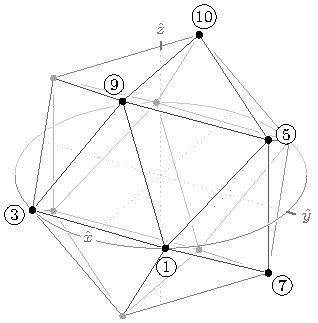
\includegraphics{figures/card_icos_sphere.pdf}}}%
  \hfil
  \COL{277pt}{\hbox to 277pt{\hfil\TAB{\CardVertexBlockA}\hskip10pt\TAB{\CardVertexBlockB}}%
    \NIS{4pt}\PBOX{277pt}{\CIdentB}}%
}%
\NIS{4pt}%
\PBOX{\hsize}{\CIdent}%
\BANDRULE
%
% --- band 2: the machine ----------------------------------------------------
\FULLHEAD{2}{\CHeadB}{\CPtrB}%
\NIS{5pt}%
\hbox to \hsize{%
  \COL{377pt}{\hbox to 377pt{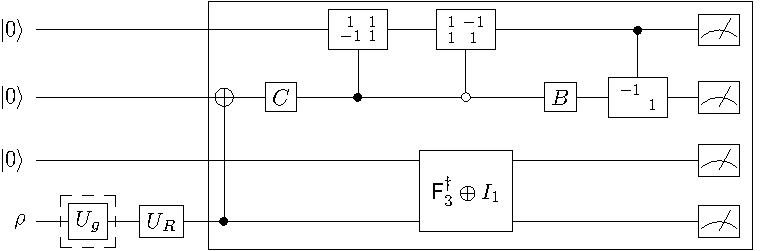
\includegraphics{figures/card_dec_icos.pdf}\hss}}%
  \hfil
  \COL{75pt}{\small\CardSide}%
}%
\NIS{5pt}%
\PBOX{\hsize}{\CParams}%
\BANDRULE
%
% --- band 3: the readout ----------------------------------------------------
\FULLHEAD{3}{\CHeadC}{\CPtrC}%
\NIS{5pt}%
\hbox to \hsize{%
  \COL{200pt}{\TAB{\CardKey}}%
  \hfil
  \COL{244pt}{\PBOX{244pt}{\CKappa}}%
}%
\BANDRULE
%
% --- band 4: the alternative ------------------------------------------------
\FULLHEAD{4}{\CHeadD}{\CPtrD}%
\NIS{5pt}%
\PBOX{\hsize}{\CRays}%
\NIS{2pt}%
\PBOX{\hsize}{\CCoin}%
}%

\caption{The solid box is \textcite[Fig.~15]{decker2004quantumcircuitssinglequbit}'s; $U_R$ and $U_g$ are ours.}
\label{fig:dec_icos_circuit}
\end{figure}

\begin{figure}[p]
% Appendix D, Figure D.5 --- "The dodecahedral POVM, end to end".  The layout only.
%
% Layout: card_oct_body.tex's header is binding.  Deviations from it, and only
% they, are listed here.
%
%   * THIS IS THE BINDING CARD, at 21.30pt of reserve: its float is the
%     tallest of the five against \textheight = 700.50687pt.  Every literal
%     in the generator's emitters is shared across the five, so any wording
%     change must be re-measured here before it ships.
%   * the ray line is the most fragile object on the five pages: ten rays,
%     443.86pt natural at \small against the 452.9679pt line -- 9.11pt of
%     slack.  Re-measure before changing any ray label.
%   * band 1 nests the worked $E_1$ under the two vertex blocks, as on the
%     icosahedron.
%   * band 2 runs 377pt + 75pt, with $B$ and $C$ in the side column; the
%     unfactored $A$ is the chapter head's (assertion 32).
%   * band 4's draw note runs to TWO lines, and every word of it is
%     measured.  "Realization forces the $\TwoI$ draw." alone is false: the
%     ten-word coin times a drawn $\{\Id, X, Y, Z\}$ flip, applied last, puts
%     forty non-group elements on both of randomness's jobs at once,
%     exactly, for half the $\Phi$ (randomized_twojobs' check_flip_completion),
%     so "forces" needs its scope ("Among groups") and the cheaper draw needs
%     saying.  The relabelling "($X$ or $Y$ swaps the pair)" may not be
%     dropped either: without the swap the four flips average the readout to
%     a multiple of $\Id$.  The wrapping is NOT read off the natural width:
%     888.29pt breaks to three lines where 880.80 still sets two, because
%     $\Id, X, Y, Z$ and $0.4\,\Phi$ cannot break.  Set the candidate in a
%     \vtop at 452.9679pt and read its DEPTH -- 2.5pt is one line, about
%     14pt is two.  A third line costs about 11pt of the reserve, so
%     re-measure before adding a word; if height is ever needed the ladder
%     below is the source.  One thing the note must not say: that a $\TwoT$
%     draw would hand this card the inscribed cube.  A $\TwoT$ draw splits
%     the ten axes 4 + 6 and the ALIGNMENT VERTEX selects which -- vertex 9,
%     this card's, selects the six, not the inscribed cube.
%   * the cut ladder, if this card must ever give height, in measured order:
%     drop the worked $E_1$ (-25.34pt); band rules 4.00 -> 3.00pt (-4.00pt);
%     the six \NIS 5 -> 4pt (-6.00pt); the key's `upper`/`lower` heads
%     (-11pt, at the cost of head 3 naming the wires again); and only as a
%     last resort \PanelScale 2.47 -> 2.20 here alone (-17pt), which forfeits
%     the uniform panel this design spends most on.
% All macros below are \def and therefore local to the figure environment.
\parindent=0pt \parskip=0pt
% Auto-generated by code/_build_povm_cards.py -- DO NOT EDIT.
% The data blocks of the dodecahedral card of Appendix D
% (paper/figures/card_dodec_body.tex \input's this and calls them).  Every
% number is derived from code/data/*.npz, Decker's circuits as
% randomized_decker rebuilds them, Figure 1.1's own \RecipeSeriesStrip, and
% Tables E.1, 5.2, D.1, D.3 and D.4, and is checked back against them before
% this file is written; see the builder's docstring for the checks (and
% _povm_cards_controls.py, which shows each of them failing on one corrupted
% literal: 100 negative controls, all aborting, 0 stale).
% Requires: booktabs, mathtools, hyperref, and the thesis macros \Id, \pmat,
% \bra, \ket, \braket, \Tr, \C, \sigmavec, \TwoT, \TwoO, \TwoI, \phig,
% \invphig, \sigmaz.  The body defines \NIS, \CTR, \PBOX, \COL, \FULLHEAD,
% \BANDRULE and \TAB, which \CardSide and the tables use.
% Regenerate with `cd code && uv run _build_povm_cards.py`.

\newcommand{\CTitle}{The dodecahedral POVM, end to end}
\newcommand{\CPtrStrip}{Introduction reference: Figure~\ref{fig:tetrahedron-recipe}}
\newcommand{\CHeadA}{Vertices and effects, $E_k = \tfrac1V(\Id + \hat n_k \cdot \sigmavec)$.}
\newcommand{\CPtrA}{Table~\ref{tab:povm-atlas} $\cdot$ Equation~\eqref{eq:povmform}}
\newcommand{\CHeadB}{Circuit; the dashed $U_g$ is an optional prepended rotation.}
\newcommand{\CPtrB}{Section~\ref{subsec:rotated-povms} $\cdot$ Table~\ref{tab:decker-pose}}
\newcommand{\CHeadC}{Register $\to$ vertex, top wire first; --- never fires}
\newcommand{\CPtrC}{Table~\ref{tab:decker-labels} $\cdot$ Section~\ref{sec:decker:using}}
\newcommand{\CHeadD}{Coin over axes, no ancilla, $\ket0$-vertex first, rightmost factor first}
\newcommand{\CPtrD}{Table~\ref{tab:decker-vs-coin} $\cdot$ Section~\ref{subsec:randomized-implementations} $\cdot$ Table~\ref{tab:binary-icosahedral-group-2i}}

\newcommand{\CStrip}{{\footnotesize\setlength{\tabcolsep}{4pt}\renewcommand{\arraystretch}{0.88}%
\begin{tabular}{@{}c c c c l l l@{}}
\toprule
$V$ & group & anc. & dead & reorientation exact? & relabelling & \hyperref[tab:decker-vs-coin]{coin over axes}\\
\midrule
20 & $\TwoI$ & 4 & 12 & no thesis gate set & permuted & 10 axes, 4 with one $\Phi$\\
\midrule
\multicolumn{7}{@{}l@{}}{only the octahedral coin is exact --- this dilation is not (Theorem~\ref{thm:main}, Appendix~\ref{sec:decker:exactness})}\\
\bottomrule
\end{tabular}}}

\newcommand{\CardVertexBlockA}{%
\begin{tabular}{@{}r l r@{}}
\toprule
$k$ & $\hat n_k$\ $(\times\tfrac{1}{\sqrt3})$ & $\bra{0}E_k\ket{0}$ \\
\midrule
$1$ & $(+1,\,+1,\,+1)$ & $0.0789$ \\
$2$ & $(+1,\,+1,\,-1)$ & $0.0211$ \\
$3$ & $(+1,\,-1,\,+1)$ & $0.0789$ \\
$4$ & $(+1,\,-1,\,-1)$ & $0.0211$ \\
$5$ & $(-1,\,+1,\,+1)$ & $0.0789$ \\
$6$ & $(-1,\,+1,\,-1)$ & $0.0211$ \\
$7$ & $(-1,\,-1,\,+1)$ & $0.0789$ \\
$8$ & $(-1,\,-1,\,-1)$ & $0.0211$ \\
$9$ & $(\phantom{+}0,\,+\invphig,\,+\phig)$ & $0.0967$ \\
$10$ & $(\phantom{+}0,\,+\invphig,\,-\phig)$ & $0.0033$ \\
\bottomrule
\end{tabular}
}

\newcommand{\CardVertexBlockB}{%
\begin{tabular}{@{}r l r@{}}
\toprule
$k$ & $\hat n_k$\ $(\times\tfrac{1}{\sqrt3})$ & $\bra{0}E_k\ket{0}$ \\
\midrule
$11$ & $(\phantom{+}0,\,-\invphig,\,+\phig)$ & $0.0967$ \\
$12$ & $(\phantom{+}0,\,-\invphig,\,-\phig)$ & $0.0033$ \\
$13$ & $(+\invphig,\,+\phig,\,\phantom{+}0)$ & $0.0500$ \\
$14$ & $(+\invphig,\,-\phig,\,\phantom{+}0)$ & $0.0500$ \\
$15$ & $(-\invphig,\,+\phig,\,\phantom{+}0)$ & $0.0500$ \\
$16$ & $(-\invphig,\,-\phig,\,\phantom{+}0)$ & $0.0500$ \\
$17$ & $(+\phig,\,\phantom{+}0,\,+\invphig)$ & $0.0678$ \\
$18$ & $(+\phig,\,\phantom{+}0,\,-\invphig)$ & $0.0322$ \\
$19$ & $(-\phig,\,\phantom{+}0,\,+\invphig)$ & $0.0678$ \\
$20$ & $(-\phig,\,\phantom{+}0,\,-\invphig)$ & $0.0322$ \\
\bottomrule
\end{tabular}
}

\newcommand{\CIdent}{$\sum_k E_k = \Id$, $\Tr E_k = \tfrac1{10}$, rank one, a $5$-design; numbered at each axis's near vertex.}
\newcommand{\CIdentB}{$E_1 = \tfrac1{20}\pmat{1+1/\sqrt3 & (1-i)/\sqrt3 \\ (1+i)/\sqrt3 & 1-1/\sqrt3}$, $E_{g(k)} = U_g E_k U_g^\dagger$.}

\newcommand{\CParams}{$U_R = R_{\hat y}(-\arccos(\phig/\sqrt{\phig+2}))$ inverts Table~\ref{tab:decker-pose}'s $R$; a drawn $U_g$ twirls and relabels outcomes by $g^{-1}$.\par\vskip1pt $A^\dagger$: Equation~\eqref{eq:adagger}; $A$: Equation~\eqref{eq:aunfactored}\par\vskip1pt $u_\pm = \sqrt{1/2 \pm \phig/(2\sqrt3)}$, $v_\pm = \mp\sqrt{1/2 \pm 1/(2\sqrt{2+\phig})}$, each $\pm1$ in the two rotation boxes is $\pm\sqrt{1/2}$\par\vskip1pt $Q_{32}^\dagger$: the CNOT $\ket{00000}\mapsto\ket{00000}$, $\ket{01001}\mapsto\ket{00001}$; $\mathsf{F}_5^\dagger \oplus I_3$, lower three wires\par\vskip1pt $\tilde{M}_{32}^\dagger = (A^\dagger \otimes (\mathsf{F}_5^\dagger \oplus I_3))\,Q_{32}^\dagger$, the Naimark extension unitary the solid box implements}

\newcommand{\CardSide}{\CTR{\hsize}{$B = \pmat{u_- & -u_+ \\ u_+ & u_-}$}\NIS{4pt}\CTR{\hsize}{$C = \pmat{v_- & v_+ \\ v_+ & -v_-}$}}

\newcommand{\CardKey}{%
\begin{tabular}{@{}c c c c c c c c c@{}}
\toprule
& \multicolumn{8}{c}{\footnotesize lower} \\
{\footnotesize upper} & $\mathtt{000}$ & $\mathtt{001}$ & $\mathtt{010}$ & $\mathtt{011}$ & $\mathtt{100}$ & $\mathtt{101}$ & $\mathtt{110}$ & $\mathtt{111}$ \\
\midrule
$\mathtt{00}$ & 17 & 3 & 11 & 9 & 1 & --- & --- & --- \\
$\mathtt{01}$ & 20 & 6 & 10 & 12 & 8 & --- & --- & --- \\
$\mathtt{10}$ & 18 & 14 & 7 & 5 & 13 & --- & --- & --- \\
$\mathtt{11}$ & 19 & 15 & 2 & 4 & 16 & --- & --- & --- \\
\bottomrule
\end{tabular}
}

\newcommand{\CKappa}{Run $U_R$ and read the key, or skip $U_R$ and read Decker's own numbered list~\cite{decker2004quantumcircuitssinglequbit}: either way $\kappa = 1$, free. His circuit with our list, index for index, is the mismatch: $\kappa = -0.009703$; under the drawn twirl it costs a $1/\kappa^2 = 10621.86\times$ premium in shots, never a bias.}

\newcommand{\CRays}{$\Phi$~$1$,\,$8$ $\cdot$ $\mathbf{F}^\dagger \Phi$~$2$,\,$7$ $\cdot$ $\Phi^\dagger \mathbf{F}^\dagger$~$3$,\,$6$ $\cdot$ $\Phi^\dagger$~$5$,\,$4$ $\cdot$ $\Id$~$9$,\,$12$ $\cdot$ $\mathbf{Z}$~$11$,\,$10$ $\cdot$ $\mathbf{F}$~$13$,\,$16$ $\cdot$ $\mathbf{F} \mathbf{X}$~$14$,\,$15$ $\cdot$ $\mathbf{F}^\dagger$~$17$,\,$20$ $\cdot$ $\mathbf{F}^\dagger \mathbf{Z}$~$19$,\,$18$}

\newcommand{\CCoin}{Draw one, apply it, then the alignment ($9 \mapsto \hat z$, inexact); measure $Z$. Among groups, realization forces $\TwoI$. With a drawn flip $\Id, X, Y, Z$ last ($X$ or $Y$ swaps the pair), these forty twirl too, at $0.4\,\Phi$, not $\TwoI$'s $0.8$.}

\long\def\NIS#1{\vskip #1\nointerlineskip}
\long\def\CTR#1#2{\hbox to #1{\hss #2\hss}}
\long\def\PBOX#1#2{\vtop{\hsize=#1\parindent0pt\sloppy\emergencystretch=1.5em\small #2}}
\long\def\COL#1#2{\vtop{\hsize=#1\parindent0pt\hbox{}\nointerlineskip #2}}
\long\def\FULLHEAD#1#2#3{\hbox to \hsize{\small\textbf{#1}\,#2\hfil{\footnotesize #3}}}
\def\BANDRULE{\vskip2pt\hrule height0.5pt\vskip1.5pt\nointerlineskip}
\long\def\TAB#1{{\small\renewcommand{\arraystretch}{0.88}\setlength{\tabcolsep}{3pt}#1}}
%
\vbox{\hsize\textwidth\parindent0pt
%
% --- title and the header strip: Figure 1.1's own row -----------------------
\hbox to \hsize{\large\bfseries \CTitle\hfil{\normalfont\footnotesize \CPtrStrip}}%
\NIS{5pt}%
\hbox{\CStrip}%
\BANDRULE
%
% --- band 1: the object -----------------------------------------------------
\FULLHEAD{1}{\CHeadA}{\CPtrA}%
\NIS{5pt}%
\hbox to \hsize{%
  \COL{170pt}{\CTR{170pt}{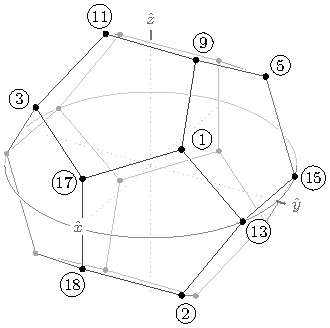
\includegraphics{figures/card_dodec_sphere.pdf}}}%
  \hfil
  \COL{277pt}{\hbox to 277pt{\hfil\TAB{\CardVertexBlockA}\hskip10pt\TAB{\CardVertexBlockB}}%
    \NIS{4pt}\PBOX{277pt}{\CIdentB}}%
}%
\NIS{4pt}%
\PBOX{\hsize}{\CIdent}%
\BANDRULE
%
% --- band 2: the machine ----------------------------------------------------
\FULLHEAD{2}{\CHeadB}{\CPtrB}%
\NIS{5pt}%
\hbox to \hsize{%
  \COL{377pt}{\hbox to 377pt{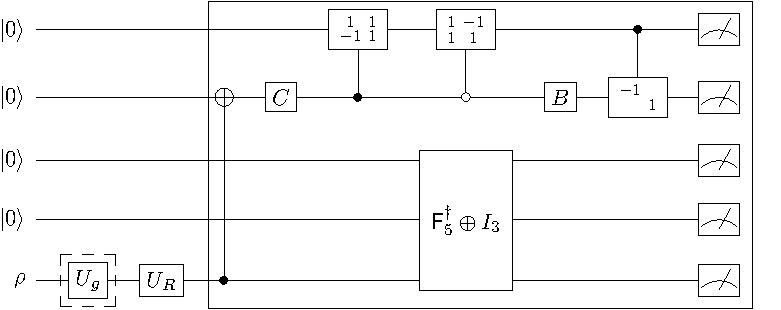
\includegraphics{figures/card_dec_dodec.pdf}\hss}}%
  \hfil
  \COL{75pt}{\small\CardSide}%
}%
\NIS{5pt}%
\PBOX{\hsize}{\CParams}%
\BANDRULE
%
% --- band 3: the readout ----------------------------------------------------
\FULLHEAD{3}{\CHeadC}{\CPtrC}%
\NIS{5pt}%
\hbox to \hsize{%
  \COL{206pt}{\TAB{\CardKey}}%
  \hfil
  \COL{238pt}{\PBOX{238pt}{\CKappa}}%
}%
\BANDRULE
%
% --- band 4: the alternative ------------------------------------------------
\FULLHEAD{4}{\CHeadD}{\CPtrD}%
\NIS{5pt}%
\PBOX{\hsize}{\CRays}%
\NIS{2pt}%
\PBOX{\hsize}{\CCoin}%
}%

\caption{The solid box is \textcite[Fig.~13]{decker2004quantumcircuitssinglequbit}'s; $U_R$ and $U_g$ are ours.}
\label{fig:dec_dodec_circuit}
\end{figure}

\clearpage % Flushes the five card floats before D.1; they are [p] and must all land first.
\makeatletter\setlength\@fptop{0pt plus 1fil}\makeatother% restores the default float-page glue
\section{Only the Octahedron Is Exactly Implementable, and Never Deterministically} \label{sec:decker:exactness}

The radicals, $\sqrt{(3\pm\sqrt{3})/12}$ for the tetrahedron and nested five-fold surds $\sqrt{\tfrac{1}{2} \pm \tfrac{1}{30}\sqrt{75 + 30\sqrt{5}}}$ for the $A_5$ solids, are forced by the geometry. (A five-fold surd for a five-fold axis.) They require a field extension no gate set here supplies. What follows quantifies over protocols, not circuits. Implementing a POVM exactly means an adaptive protocol's effects \textit{are} the POVM's, and a Platonic solid POVM's are rank one by Equation~\eqref{eq:povmform}. Circuits do arithmetic: composing gates only adds and multiplies matrix entries, so a circuit never leaves the ring its gates' entries generate---for unitaries, this is exact synthesis. We take this arithmetic from unitaries to POVMs, through ancillas, coins, feedforward and discarding---a discarding protocol's surviving effects summing to a multiple of $\Id$, its outcomes reported conditioned on acceptance. We find two obstructions. A rank-one effect's direction must land in one real field, the same in every pose, so the number that convicts a solid need not be Decker's---for the dodecahedron it is $\sqrt{3}$, no five-fold surd at all. And a deterministic protocol's weights must land in the ring itself, a denominator obstruction no field can see ($\tfrac{1}{3}$ and $1$ are equally at home in $\mathbb{Q}$). Section~\ref{sec:decker:statements} states the results with proof sketches, and Section~\ref{sec:decker:exactness:expanded} proves the two the sketches cannot carry: the octahedron's construction and the weight obstruction. The whole argument at reading pace is in \texttt{extras/math/} in the repository. Table~\ref{tab:decker-vs-coin} lists each solid's realizing coin (Section~\ref{subsec:randomized-implementations}), including the octahedron's three-word construction.

Throughout, $\mathcal{R} \subset \C$ is a subring containing $i$ and closed under complex conjugation, $K = \operatorname{Frac}\mathcal{R}$ its field of fractions and $K_\R = K \cap \R$ the real subfield. The circuits will stay inside $\mathcal{R}$, and only the reading of a direction will step out, into $K_\R$.

% Auto-generated by code/randomized_implementations.py.
% Include this file with \input{...}.
% Requires: \usepackage{booktabs}, \usepackage{float}, and the thesis
% macros \TwoT, \TwoO, \TwoI, \Tgroup, \Ogroup, \Igroup, \Id,
% \Tr, \SO, \R, \phig.
% Regenerate with `cd code && uv run randomized_implementations.py`.

\begin{table}[H]\centering
\small
\setlength{\tabcolsep}{6pt}
\renewcommand{\arraystretch}{1.2}
\begin{tabular}{l l c c}
\toprule
 & & \multicolumn{2}{c}{Coin cost} \\
\cmidrule(lr){3-4}
POVM ($V$) & Coin words (min-$\Phi$) & Depth & $\Phi$ \\
\midrule
  Tetrahedron (4) & --- (indecomposable; the dilation is forced) & --- & --- \\
  Octahedron (6) & $\Id$, $\mathbf{F}$, $\mathbf{F}^\dagger$ & $\le 1$ & $0$ \\
  Cube (8) & $\Id$, $\mathbf{F}$, $\mathbf{Z}$, $\mathbf{F}^\dagger$ & $\le 1$ & $0$ \\
  Icosahedron (12) & $\Id$, $\mathbf{F}$, $\mathbf{X}$, $\mathbf{F}^\dagger$, $\mathbf{X} \mathbf{F}$, $\mathbf{X} \mathbf{F}^\dagger$ & $\le 2$ & $0$ \\
  Dodecahedron (20) & $\Id$, $\mathbf{F}$, $\mathbf{Z}$, $\mathbf{F}^\dagger$, $\mathbf{F} \mathbf{X}$, $\mathbf{F}^\dagger \mathbf{Z}$, $\Phi$, $\Phi^\dagger$, $\mathbf{F}^\dagger \Phi$, $\Phi^\dagger \mathbf{F}^\dagger$ & $\le 2$ & $\le 1$ \\
\bottomrule
\end{tabular}
\caption{The realizing coin over axes: one atlas circuit per Platonic solid POVM vertex axis (min-$\Phi$ synthesis, one word per antipodal pair). A uniform draw reproduces the POVM's effects exactly. These words replace Decker's ancilla register; what they do not replace is the fixed \textit{alignment} rotation every projective shot applies after the drawn word, on which the field demand of Table~\ref{tab:implementation-ledger} is paid---the identity for the octahedron, inexact for every other solid (Theorem~\ref{thm:main}). The cost columns price this realizing coin alone; Table~\ref{tab:implementation-ledger}'s \textit{draw} costs more because a single draw must also twirl, which no group below order $12$ can do. (For the dodecahedron the gap is forced by transitivity rather than by the twirl; Section~\ref{sec:povmsinuse}.)}
\label{tab:decker-vs-coin}
\end{table}


\subsection{Statements} \label{sec:decker:statements}

Call a gate set \textit{admissible} if every one of its gates has entries in $\mathcal{R} = \mathbb{Z}[\phig, i, \sqrt{2}, \tfrac{1}{2}]$. Its field of fractions is $K = \mathbb{Q}(\sqrt{2},\sqrt{5},i)$, the smallest field holding every entry of Table~\ref{tab:complexity_hierarchy}'s Algebraic Field row, whence $K_\R = \mathbb{Q}(\sqrt{2},\sqrt{5})$. Every gate set of this thesis is admissible and contains $\TwoT$: $\TwoT$, Clifford, Clifford${}+T$, $\TwoI$, Clifford${}+\Phi$, and their unions, each adjoined with an entangling Clifford such as CNOT, whose $0$'s and $1$'s change nothing.

\begin{theorem} \label{thm:main}
Over any admissible gate set, of the five Platonic solid POVMs only the octahedral is exactly implementable, i.e., with no approximation, by a protocol in the sense of Lemma~\ref{lem:branch}: the other four in no pose, the octahedron at least in atlas orientation over any set containing $\TwoT$, where its vertices are the Pauli axes. Over any admissible gate set, no deterministic protocol in the sense of Theorem~\ref{thm:weight}, hence no dilation, implements any of the five exactly: the octahedron's exactness costs a coin, a discarded branch, or unbounded repetition.\footnote{Cf.\ the no-go over a strictly narrower model~\cite[Thm.~1]{monaco2025nonstabilizernesscostquantum}: one fixed Clifford unitary, stabilizer ancillas, a stabilizer-basis readout and no coin never realize an informationally complete POVM, where the three-word coin of Table~\ref{tab:decker-vs-coin} realizes one, every effect $\tfrac13$ of a stabilizer projector.}
\end{theorem}

\begin{sketch}
Four impossibilities by arithmetic plus one construction: Lemmas~\ref{lem:witness} and~\ref{lem:membership} with Table~\ref{tab:povm-exactness} put the other four solids' witness outside $K_\R$ in every pose, where Corollary~\ref{cor:directions} bans them, while the octahedron's Pauli axes are realized by a three-word coin from $\TwoT$. For the octahedron, determinism fails separately: by Theorem~\ref{thm:weight}, a deterministic protocol has dyadic weights only, and its effects weigh $\tfrac{1}{3}$.
\end{sketch}

\begin{lemma}[branch decomposition] \label{lem:branch}
Let $\mathcal{R} \subset \C$ contain $i$ and be closed under complex conjugation, let a gate set have all its matrix entries in $\mathcal{R}$, and consider any protocol built from it: one data qubit, finitely many ancillas prepared in $\ket{0}$, gates from the set, computational-basis measurements, classical coins of arbitrary bias, feedforward (later gates conditioned on earlier coins and outcomes), and classical post-processing assigning at most one label per record, a randomized labelling being one more coin. Every effect it realizes decomposes as
\begin{equation*}
E_k \;=\; \sum_{b} p_b \ketbra{a_b}{a_b}, \qquad \ket{a_b} \in \mathcal{R}^2, \quad p_b > 0,
\end{equation*}
one term per \textit{branch} $b$, a branch being one complete record of coin values and measurement outcomes that post-processing labels $k$, with $p_b$ the product of the coin probabilities along $b$. If the protocol tosses no coin, every $p_b = 1$.\footnote{For \textit{unitaries} the analogous characterization is classical, and finer, exact synthesizability being decided by \textit{ring} membership of the entries~\cite{kliuchnikov2013fastefficientexacta,giles2013exactsynthesismultiqubit,kliuchnikov2015frameworkexactsynthesis}, \textcite[\S2.4]{forest2015exactsynthesissinglequbit} giving the $\SO(3)$ form from which Corollary~\ref{cor:alignment}'s gate-level variant is immediate. Here the object is the adaptive measurement protocol and its rank-one effects; the nearest prior statement is that a repeat-until-success circuit over Clifford${}+T$ reaches only unitaries over $\mathbb{Z}[i,\sqrt{2}]$ \textit{after multiplication by a scalar}~\cite[\S3.1]{paetznick2014repeatuntilsuccessnondeterministicdecomposition}, the same conditioning on a branch. Heralded protocols reach the whole fraction field~\cite[Cor.~21]{bocharov2015efficientsynthesisuniversala}, which the lemma survives by being projective, the escaping scalar absorbed into $c$, which Corollary~\ref{cor:directions} does not constrain; and the $\ket{0}$ ancillas keep every branch in $\mathcal{R}$, where a catalyst outside it would not~\cite[\S VI\,B]{amy2023catalyticembeddingsquantum}.}
\end{lemma}

\begin{sketch}
Condition on a branch and every fork is decided, leaving one definite sequence of gates, $0/1$ projectors and $\ket{0}$ ancillas; composing them only adds, multiplies and conjugates entries, which never leaves $\mathcal{R}$, and the coins contribute no operator at all---only the scalar $p_b$.
\end{sketch}

The lemma has two readings. Its \textit{weights} $\Tr[E_k]$ stay in $\mathcal{R}$ under a deterministic protocol (Theorem~\ref{thm:weight}); its \textit{directions}, the Bloch vectors $\hat n$, divide once, and land in $K_\R^3$ either way. What separates the two readings is the coin, the discarded branch, or unbounded repetition. Theorem~\ref{thm:weight} is the only statement here that needs any of the three: banning the discard makes the outcome classes partition the branches, bounding the rounds keeps them finitely many. The rest count no branches, and never ask the effects to sum to $\Id$.

% Letters in Appendix D: $w$ stays out --- it already means the quaternion real part (Ch.~2, App.~A, App.~C latitude), the Pauli-string weight (App.~F) and Algorithm~\ref{alg:dijkstra_gen}'s gate sequence. \textit{Weight} names $\Tr[E_k]$ throughout D.1, symbolized at its definition point in Theorem~\ref{thm:weight}; the positive multiple in front of $\ketbra{\psi}{\psi}$ is representative-dependent ($\ket{\psi}$ must stay unnormalized to stay in $\mathcal{R}^2$), so it is called \textit{the multiple} or \textit{the scale} and never a weight --- in print it carries the letter $c$, defined in Corollary~\ref{cor:directions}, which leaves it unconstrained, and $c \notin \mathcal{R}$ in general even where the effect's weight is. The weights $p_b$ of the protocol's branches are untouched. Prefer symbols over words here.
\begin{corollary}[directions] \label{cor:directions}
Any rank-$1$ effect such a protocol realizes is $c\ketbra{\psi}{\psi}$ for some $c > 0$ and some $\ket{\psi} \in \mathcal{R}^2$, and its Bloch vector $\hat n$ lies in $K_\R^3$. Neither $c$ nor $p_b$ need lie in $\mathcal{R}$.\footnote{None of this is about \textit{simulability}: with an ancilla of the system's own dimension, projective measurements and classical randomness reproduce the statistics of any POVM~\cite[Thm.~1]{oszmaniec2017simulatingpositiveoperatorvaluedmeasures}, but there the measurements may point anywhere, and the constraint here is which directions a gate set can build.}
\end{corollary}

\begin{sketch}
Rank one forces all the $\ket{a_b}$ parallel, so the effect has one direction over $\mathcal{R}$; its Bloch coordinates divide by $\braket{\psi}{\psi}$ and so land in $K_\R$, which is blind to the weight that division removed.
\end{sketch}

\begin{theorem}[weights] \label{thm:weight}
Call a protocol \textit{deterministic} if it tosses no classical coin, discards no branch, and halts within a bounded number of rounds, every run returning an outcome; feedforward is still allowed. A deterministic protocol realizes only effects whose \textit{weight} $\Tr[E_k]$ lies in $\mathcal{R}$. For $\mathcal{R} = \mathbb{Z}[\phig, i, \sqrt{2}, \tfrac{1}{2}]$ the rationals in $\mathcal{R}$ are the dyadics $\mathbb{Z}[\tfrac{1}{2}]$, so a transitive covariant qubit POVM on $V$ outcomes admits a deterministic implementation only if $V$ is a power of two.\footnote{Decker's dilations are therefore optimal on the only terms open to a dilation: within the Naimark construction the register cannot shrink---more than $d$ vectors in $\C^d$ cannot be mutually orthogonal, so $V$ outcomes need dimension at least $V$~\cite[\S2]{decker2005implementationgroupcovariantpositive}---and the radicals inside $A^\dagger$ cannot rationalize. Neither can they be relocated: the construction leaves the completing unitary, the POVM vectors' order and phases, a permutation of the irreducibles and a restriction to a subgroup all free, but not the block the POVM determines, the freedom living in the rows that block does not occupy~\cite[\S5 and Ex.~7]{decker2005implementationgroupcovariantpositive}. Both obstructions quantify over protocols and over the POVM, never over a circuit.}
\end{theorem}

\begin{sketch}
Ban the coin and every $p_b$ is $1$; ban the discard and no renormalization follows, so no division intervenes here; given a bounded number of rounds, $\Tr[E_k]$ is a \textit{finite} sum over $\mathcal{R}$, hence in $\mathcal{R}$; $\mathcal{R}$'s members being algebraic integers over a power of two makes $\mathcal{R} \cap \mathbb{Q}$ the dyadics, and transitive covariance makes $\Tr[E_k] = 2/V$.
\end{sketch}

\begin{lemma}[rotation-proof witness] \label{lem:witness}
Let $v_1,\dots,v_n$ span $\R^3$ with all inner products in $K_\R$. Then for an independent triple, $\det[v_a\,v_b\,v_c] \in K_\R$ exactly when the Gram determinant $\det\Gamma_{abc}$ is a square in $K_\R$; independent triples share a square class, so any one of them decides. Inner products are unchanged by $\mathrm{O}(3)$, so the verdict is the same in every pose.
\end{lemma}

\begin{sketch}
A triple's determinant is unmoved by rotation and squares to their Gram determinant, so if any pose put every vertex in $K_\R^3$ the number computed in the pose at hand would already lie in $K_\R$; and passing between spanning triples multiplies the Gram determinant by a square, so one triple decides for the solid.
\end{sketch}

\begin{lemma}[membership in $K_\R$] \label{lem:membership}
For $K_\R = \mathbb{Q}(\sqrt{2},\sqrt{5})$ and squarefree $d > 1$, $\sqrt{d} \in K_\R$ if and only if $d \in \{2,5,10\}$; in particular $\sqrt{3} \notin K_\R$. If $\alpha \in \mathbb{Q}(\sqrt{5})$ is a square in $K_\R$, then at least one of $\alpha$ and $\alpha/2$ is a square in $\mathbb{Q}(\sqrt{5})$, and that one's field norm is a rational square---so if neither norm is a rational square, $\alpha$ is not a square in $K_\R$. Neither $\tfrac{2}{25}(5-\sqrt{5})$ nor $\tfrac{1}{2}(5+\sqrt{5}) = 2 + \phig$ is a square in $K_\R$. Outsiders come in cosets: for real $\xi \neq 0$ and nonzero $\nu \in K_\R$, each of $\nu\xi$ and $\nu/\xi$ lies in $K_\R$ exactly when $\xi$ does, so the ban on $\sqrt{3}$ and $\sqrt{2+\phig}$ reaches their nonzero $K_\R$-multiples and quotients.
\end{lemma}

\begin{sketch}
Write $\sqrt{d} = p + q\sqrt{2}$ with $p, q \in \mathbb{Q}(\sqrt{5})$; squaring forces $pq = 0$, and the same coefficient comparison, now for $\mathbb{Q}(\sqrt{5})$ over $\mathbb{Q}$, leaves one of $d$, $2d$, $5d$, $10d$ a rational square---for squarefree $d$, that pins $d \in \{2, 5, 10\}$. The five-fold surds enter squared, and $\alpha = \beta^2$ splits the same way: $\alpha$ or $\alpha/2$ is a square in $\mathbb{Q}(\sqrt{5})$, whose field norm $a^2 - 5b^2$ must then be a rational square---and all four candidates fail on squarefree part $5$. The coset clause is closure forward, and $\xi = (\nu\xi)/\nu = \nu/(\nu/\xi)$ backward.
\end{sketch}

% Auto-generated by code/randomized_implementations.py.
% Include this file with \input{...}.
% Requires: \usepackage{booktabs}, \usepackage{float}, and the thesis
% macros \TwoT, \TwoO, \TwoI, \Tgroup, \Ogroup, \Igroup, \Id,
% \Tr, \SO, \R, \phig.
% Regenerate with `cd code && uv run randomized_implementations.py`.

\begin{table}[h]\centering
\renewcommand{\arraystretch}{1.2}
\begin{tabular}{l c c c c}
\toprule
Solid & $(a,b,c)$ & $\det[v_a\,v_b\,v_c]$ & Minimal polynomial & Demands \\
\midrule
  Tetrahedron & $(1,2,3)$ & $-4\sqrt{3}/9$ & $27 x^{2} - 16$ & $\sqrt{3}$ \\
  Octahedron & $(1,3,5)$ & $+1$ & $x - 1$ & --- (none) \\
  Cube & $(1,2,3)$ & $-4\sqrt{3}/9$ & $27 x^{2} - 16$ & $\sqrt{3}$ \\
  Icosahedron & $(1,2,5)$ & $+\tfrac{1}{5}\sqrt{10-2\sqrt{5}}$ & $125 x^{4} - 100 x^{2} + 16$ & $\sqrt{5+2\sqrt{5}}$ \\
  Dodecahedron & $(1,2,3)$ & $-4\sqrt{3}/9$ & $27 x^{2} - 16$ & $\sqrt{3}$ \\
\midrule
\multicolumn{5}{c}{One extension, three names: $\sqrt{5+2\sqrt{5}} = \phig\sqrt{2+\phig}$ and $\sqrt{10-2\sqrt{5}} = (2/\phig)\sqrt{2+\phig}$.} \\
\bottomrule
\end{tabular}
\caption{The exactness obstruction. Here $v_a, v_b, v_c$ is the solid's first vertex triple spanning $\R^3$, numbered and posed as in Appendix~\ref{sec:povm-atlas:vertices}. The triple is a choice, but every spanning triple's determinant is a $K_\R$-multiple of the one shown, so any one decides (Lemma~\ref{lem:witness}), and the determinant is unchanged by rotation, so no pose escapes the test. The minimal polynomial pins each determinant exactly; degree four alone bars nothing, $K_\R$ having degree four, and Lemma~\ref{lem:membership} gives the verdict, barring all three surds of the footer row by naming $2+\phig = \tfrac{1}{2}(5+\sqrt{5})$ and the determinant's square. Only the octahedron survives this test. Computed symbolically by \texttt{code/randomized\_implementations.py}.}
\label{tab:povm-exactness}
\end{table}


\begin{corollary}[alignment] \label{cor:alignment}
In atlas orientation (Table~\ref{tab:povm-atlas}), no protocol over an admissible gate set measures projectively along any vertex of the tetrahedron, cube, icosahedron, or dodecahedron exactly.
\end{corollary}

\begin{sketch}
Both effects of a projective measurement along a vertex $\hat v$ are rank $1$ with Bloch vectors $\pm\hat v$, so Corollary~\ref{cor:directions} puts $\hat v$ in $K_\R^3$. Swept per vertex (\texttt{code/randomized\_implementations.py}), every nonzero coordinate of a tetrahedron, cube or dodecahedron vertex is $p/\sqrt{3}$ with $\abs{p} \in \{1, \invphig, \phig\}$, and of an icosahedron vertex $p/\sqrt{2+\phig}$ with $\abs{p} \in \{1, \phig\}$; Lemma~\ref{lem:membership} bans both surds, and its coset clause carries the ban to these quotients.
\end{sketch}

\subsection{Two proofs} \label{sec:decker:exactness:expanded}

% This subsection proves Section~\ref{sec:decker:statements}'s statements, so it must carry their notation: the branch index is $b$, the multiple is $c$ (defined in Corollary~\ref{cor:directions}), and the effect weight is $\Tr[E_k]$ (see the note there). Keep all three on any future edit.
% The slow walk (the refresher on the ring, the protocol model, the $K_\R$ refresher, the witness, the three doors' arithmetic, the alignment corollary slowly, the axis dictionary) is in extras/math/exactness-slow-walk.tex, and the notation note above binds that document too; what stays here is the octahedron's construction and Theorem~\ref{thm:weight}'s proof.

\begin{proof}[The octahedron, exhibited]
Draw a word $W$ uniformly from $\{\Id, \mathbf{F}, \mathbf{F}^\dagger\}$ (Table~\ref{tab:decker-vs-coin}), apply it, measure $Z$, and report both the word and the sign $\pm$. The effect for the label $(W, \pm)$ is $\tfrac{1}{3}W^\dagger\tfrac{1}{2}(\Id \pm \sigmaz)W$. Now $F = HS^\dagger$ acts on the Bloch sphere as the $3$-cycle $\hat x \to \hat y \to \hat z \to \hat x$, so the conjugates $W^\dagger\sigmaz W$ are $\sigmaz$, $\sigma_y$, $\sigma_x$ in turn, and the six effects are $\tfrac{1}{6}(\Id \pm \sigma_a)$ for $a \in \{x, y, z\}$. Against the definition: each is rank $1$, their directions are the Pauli axes, each has trace $\tfrac{1}{3} = 2/6$, and they sum to $\Id$. That is the octahedral POVM in atlas orientation, exactly. And $F$ lies in $\TwoT$ up to phase (the symmetrized $\mathbf{F} = e^{-i\pi/4}F$ is the group element, and a conjugation cannot see a global phase), and every gate set of this thesis contains $\TwoT$, so the construction is available over all of them---nothing approximated, no $T$ and no $\Phi$ required. Theorem~\ref{thm:main}'s first sentence is now proved in both directions: four solids ruled out by arithmetic, the fifth built, at the weight $\tfrac13$ Theorem~\ref{thm:weight} convicts.
\end{proof}

\begin{proof}[Proof of Theorem~\ref{thm:weight}]
The yardstick is the \textit{algebraic integer}, a root of a monic polynomial with integer coefficients; the only rational ones are the integers, and they are closed under $+$ and $\times$~\cite[Lem.~13.1.1, Exercise~13.1.3(a) and Ex.~14.M.8(c)]{artin2011algebra}. Every generator of $\mathcal{R} = \mathbb{Z}[\phig, i, \sqrt{2}, \tfrac{1}{2}]$ is an algebraic integer over a power of two, so every member is, and $\mathcal{R} \cap \mathbb{Q} = \mathbb{Z}[\tfrac{1}{2}]$, the dyadics. Ban the coin, and every $p_b$ is $1$; a randomized labelling is a coin too, and for rank-one effects Corollary~\ref{cor:directions} defeats it regardless: the effect of every label a branch feeds is a multiple of $\ketbra{a_b}{a_b}$, and the solids' vertices are distinct, so each branch feeds one label only, hence with probability $1$. Ban the discard and bound the rounds, and no division intervenes (the direction-reading division of Corollary~\ref{cor:directions} was ours); so, Lemma~\ref{lem:branch} having run over $\mathcal{R}$, the trace $\Tr[E_k] = \sum_b \braket{a_b}{a_b}$ is a finite sum over $\mathcal{R}$ and its conjugates, a real member of $\mathcal{R}$. Transitive covariance (Section~\ref{subsubsec:platonic-transitive}) makes the effects one orbit of equal weight, totalling $\Tr[\Id] = 2$, so $\Tr[E_k] = 2/V$ is rational, hence dyadic, and $V$ is a power of two: the tetrahedron ($\tfrac{1}{2}$) and the cube ($\tfrac{1}{4}$) pass, and fail the vertex test instead; the octahedron ($\tfrac{1}{3}$), icosahedron ($\tfrac{1}{6}$) and dodecahedron ($\tfrac{1}{10}$) fail outright, as \texttt{code/randomized\_implementations.py} confirms solid by solid. This is Theorem~\ref{thm:main}'s second sentence: no deterministic protocol (any dilation, Decker's or the coin-free construction of~\cite[Eq.~(8)]{yordanov2019implementationgeneralsinglequbit} included) implements any of the five exactly.
\end{proof}

The coin in the exhibition is interchangeable with a discarded branch or with unbounded repetition (Figure~\ref{fig:protocol-doors}): each realizes the weight $\tfrac13$ exactly, and Theorem~\ref{thm:weight} excludes each. Excluding the discard (i.e., \textit{postselection}) is not arbitrary: a POVM answers every shot, so its effects sum to $\Id$ with no acceptance probability to divide by. Corollary~\ref{cor:directions} counts no branches, so the other four solids stay banned under all three; the octahedron's weight $\tfrac13$ is all that randomization provides.

\begin{figure}[htbp]
\centering
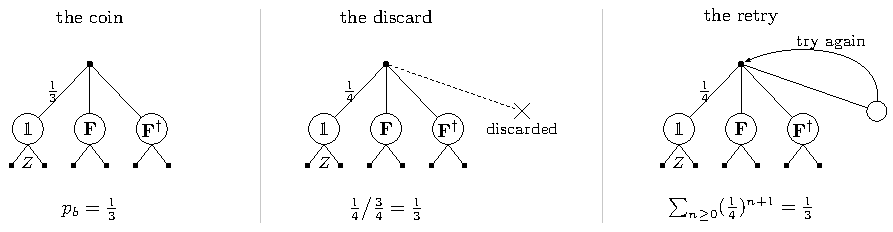
\includegraphics{figures/protocol_doors.pdf}
\caption{Three realizations of the weight $\tfrac13$: the octahedron's exhibition with one classical edge changed. The coin draws three branches at probability $\tfrac13$ each. The discard draws four at dyadic weight $\tfrac14$ and deletes one, reaching $\tfrac13$ as a ratio of acceptance probabilities; the acceptance probability is state-independent, so the conditional statistics are exactly the POVM's. The retry returns that branch to the root instead, reaching $\tfrac13$ as a limit of dyadic partial sums, at $\tfrac43$ expected rounds. All three realize $\tfrac{1}{6}(\Id \pm \sigma_a)$ exactly, so \textit{deterministic} in Theorem~\ref{thm:weight} must exclude each separately. Verified in \texttt{code/weight\_obstruction\_escapes.py}.}
\label{fig:protocol-doors}
\end{figure}

In atlas orientation, then, a Platonic solid POVM is exactly implementable, never deterministically, if and only if its vertices are the Pauli axes: the other four solids' vertices sit on the rotation axes of $F$ and $\Phi$, whose eigenstates are magic states~\cite[Def.~1 and Fig.~1]{bravyi2005universalquantumcomputation}, non-constructible by Clifford means for the same field-theoretic reason~\cite[Thm.~1 and \S3.2]{veitch2014resourcetheorystabilizer}.


\section{Reorientation and Relabelling} \label{sec:decker:using}

Two things stand between the solid-boxed circuits of the figures above and the POVMs of Section~\ref{sec:platonic-solid-povms}. This section derives both corrections---the prefix $U_R$ of those figures, and the outcome relabelling they record---and prices them. The first is orientation. Decker parks the solid's cyclic symmetry axis on $\hat z$, and the size of his Fourier block $\mathsf{F}_m$ is the order of that axis; ours is read off Figure~\ref{fig:platonic-solid-povms}, the order of each feature being its stabilizer in Table~\ref{tab:permutation-structure}. Table~\ref{tab:decker-pose} holds the comparison.

% Permutations and premiums live in Table~\ref{tab:decker-labels} below (emitted, data/randomized_labels.tex), whose cells are bare. The permutation column prints because a card's rectangle key needs base-2 decoding while the column reads at sight; the fragment's ``% key'' comment lines stay for the card and recipe builds.
\begin{table}[h]
\centering
\begin{tabular}{@{} l c c l c @{}}
\toprule
Solid & Decker's $\hat z$ & Our $\hat z$ & A reorientation $R$, exact? & Outcomes \\
\midrule
Tetrahedron  & edge, $2$ ($\mathsf{F}_2$)   & edge, $2$   & $R_z(45^\circ)$, over Clifford${}+T$ & $k \mapsto k$ \\
Octahedron   & face, $3$ ($\mathsf{F}_3$)   & vertex, $4$ & $R_z(45^\circ)R_y(\arccos(1/\sqrt3))R_z(180^\circ)$, no & permuted \\
Cube         & face, $4$ ($\mathsf{F}_4$)   & face, $4$   & $R_z(45^\circ)$, over Clifford${}+T$ & permuted \\
Icosahedron  & face, $3$ ($\mathsf{F}_3$)   & edge, $2$   & $R_y(-\arccos(1/(\phig\sqrt3)))$, no & permuted \\
Dodecahedron & face, $5$ ($\mathsf{F}_5$)   & edge, $2$   & $R_y(\arccos(\phig/\sqrt{\phig+2}))$, no & permuted \\
\bottomrule
\end{tabular}
\caption{Decker's orientation against ours (Table~\ref{tab:povm-atlas}): the feature each $\hat z$ passes through and the order of the rotation about it, his the size of the $\mathsf{F}_m$ block~\cite[\S\S4, 6--10]{decker2004quantumcircuitssinglequbit}, ours read off Figure~\ref{fig:platonic-solid-povms}. The reorientation $R$ carries his solid onto ours, one representative of a coset of the solid's rotation group ($12$, $24$, $24$, $60$, and $60$ members, none an atlas word), exact over the gate set named, if any; the prefix $U_R$ realizing it has Bloch rotation $R^{-1}$, and \textit{Outcomes} records whether it also preserves the outcome labelling. Computed in \texttt{code/randomized\_implementations.py}.}
\label{tab:decker-pose}
\end{table}

Two of the reorientations are turns about $\hat y$ and two about $\hat z$ itself; the octahedron's is not a rotation about a coordinate axis (Figure~\ref{fig:dec_oct_circuit}). Decker stands each solid on its own, so neither dual pair is actually dual-aligned in his poses; we pose the five as a family, keeping both pairs. Reorienting comes at two prices: the operation over a fixed gate set, and, larger by up to four orders of magnitude, not noticing it was needed.

The second thing to correct is labelling. A reorientation carries vertices to vertices but not indices to indices, and only the tetrahedron is lucky: exactly one of the twelve possible reorientations sends outcome $k$ to vertex $k$ of Table~\ref{tab:povm-atlas}, and it is the one drawn in Figures~\ref{fig:tet_povm_circuit} and~\ref{fig:dec_tet_circuit}. For the remaining four solids, no reorientation preserves outcome order, so each needs a fixed permutation applied in post-processing: classical bookkeeping, free but not optional; printed in each figure and in Table~\ref{tab:decker-labels}.

The upshot: apply both corrections, and the atlas rows are POVM rotations; or neither, and keep Decker's pose and vertex list. A mismatch costs, and Table~\ref{tab:decker-labels} prices it.

A reorientation needs no exactness the circuit never had, Lemma~\ref{lem:witness} being rotation-proof and weights not geometric, and it leaves the twirl's factor alone. Run twirled-native unreoriented and the estimator stays unbiased under the same estimator-channel factor $\Tr[T]/3$, Schur wanting irreducibility and nothing more; the snapshots (the sampled vertices, Appendix~\ref{sec:shadows:setup}) must then be read against Decker's vertices, and handing the estimator our list instead moves the factor, which Table~\ref{tab:decker-labels} prices.

% $\kappa$ is defined in Table~\ref{tab:decker-labels}'s caption (emitted, data/randomized_labels.tex), with the failure modes and the misattribution warning; the $\kappa = 3\eta$ dictionary prints in Section~\ref{sec:shadows:belief}, so this caption stays dictionary-free by design and carries only the scale-guard sentence.
% Do not price the reorientation \textit{rotation} alone: valid reorientations form a left coset $G R_0$ with $\kappa(h) = \Tr(h R_0)/3$, whose mean is $0$ and mean-square $1/9$ universally --- any solid, any pose --- so a single member is never ``the'' figure. Table~\ref{tab:decker-labels}'s numbers price rotation $\circ$ labelling, which is what running his circuit actually costs; all five land inside their coset ranges, the tetrahedron exactly at its maximum (it is the one solid whose outcome order survives) and the cube exactly at its minimum.
% A general outcome permutation is laundered to a scalar too --- over a uniformly random relabelling $\mathbb{E}[\kappa] = 0$ and $\mathbb{E}[\kappa^2] = 1/(3(V-1))$ exactly --- so a scrambled label is worse on a bigger POVM. This does not print; if it ever does, $\kappa$ stays bare and the relabelling clause with it, since $\pi$ is the representation of Section~\ref{subsec:schur} and the constant everywhere else, never a permutation.

% Auto-generated by code/randomized_implementations.py.
% Include this file with \input{...}.
% Requires: \usepackage{booktabs}, \usepackage{float}, and the thesis
% macros \TwoT, \TwoO, \TwoI, \Tgroup, \Ogroup, \Igroup, \Id,
% \Tr, \SO, \R, \phig.
% Regenerate with `cd code && uv run randomized_implementations.py`.

% The register-to-vertex key of each solid, live computational
% outcome (from 0) -> our vertex (from 1); printed in the table
% below and on the cards, read here by code/_build_povm_cards.py
% and code/_build_recipe_figure.py.
% key tetrahedron: 0 1 2 3 -> 1 2 3 4
% key octahedron: 0 1 2 4 5 6 -> 5 3 1 6 4 2
% key cube: 0 1 2 3 4 5 6 7 -> 7 8 5 6 1 2 3 4
% key icosahedron: 0 1 2 4 5 6 8 9 10 12 13 14 -> 10 4 2 11 1 3 9 8 7 12 5 6
% key dodecahedron: 0 1 2 3 4 8 9 10 11 12 16 17 18 19 20 24 25 26 27 28 -> 17 3 11 9 1 20 6 10 12 8 18 14 7 5 13 19 15 2 4 16
\begin{table}[h]\centering
\small
\setlength{\tabcolsep}{5pt}
\renewcommand{\arraystretch}{1.2}
\begin{tabular}{l l c c}
\toprule
Solid & Outcome (from $0$) $\mapsto$ our vertex (from $1$) & $\kappa$ & $1/\kappa^{2}$ \\
\midrule
  Tetrahedron & $\bigl(\begin{smallmatrix} 0 & 1 & 2 & 3 \\ 1 & 2 & 3 & 4 \end{smallmatrix}\bigr)$ & $+0.804738$ & $1.54$ \\
  Octahedron & $\bigl(\begin{smallmatrix} 0 & 1 & 2 & 4 & 5 & 6 \\ 5 & 3 & 1 & 6 & 4 & 2 \end{smallmatrix}\bigr)$ & $+0.321975$ & $9.65$ \\
  Cube & $\bigl(\begin{smallmatrix} 0 & 1 & 2 & 3 & 4 & 5 & 6 & 7 \\ 7 & 8 & 5 & 6 & 1 & 2 & 3 & 4 \end{smallmatrix}\bigr)$ & $-1/3$ exactly & $9.00$ \\
  Icosahedron & $\bigl(\begin{smallmatrix} 0 & 1 & 2 & 4 & 5 & 6 & 8 & 9 & 10 & 12 & 13 & 14 \\ 10 & 4 & 2 & 11 & 1 & 3 & 9 & 8 & 7 & 12 & 5 & 6 \end{smallmatrix}\bigr)$ & $+0.116566$ & $73.60$ \\
  Dodecahedron & $\bigl(\begin{smallmatrix} 0 & 1 & 2 & 3 & 4 & 8 & 9 & 10 & 11 & 12 & 16 & 17 & 18 & 19 & 20 & 24 & 25 & 26 & 27 & 28 \\ 17 & 3 & 11 & 9 & 1 & 20 & 6 & 10 & 12 & 8 & 18 & 14 & 7 & 5 & 13 & 19 & 15 & 2 & 4 & 16 \end{smallmatrix}\bigr)$ & $-0.009703$ & $10621.86$ \\
\bottomrule
\end{tabular}
\caption{Decker's outcome order, and the price of ignoring it. The permutation column records, in two-line notation, the relabelling owed once the reorientation of Table~\ref{tab:decker-pose} is applied: the top row holds the live computational outcomes of Figures~\ref{fig:dec_tet_circuit}--\ref{fig:dec_dodec_circuit}, top wire first, and beneath each is the vertex it then fires as, numbered from $1$ as in Appendix~\ref{sec:povm-atlas:vertices}; outcomes absent from a top row are dead and never fire. This permutes Decker's own printed vertex numbering, which the adapted circuits reproduce. Run $U_R$ and relabel, or skip $U_R$ and read Decker's own numbered list: either way $\kappa = 1$. The column prices a mismatch, his circuit as published with our list, index for index. No misspecified belief can tilt a twirled estimator: the estimator channel is $\kappa\,\Id$ with zero offset, $\kappa$ the overlap of the believed vertex list with the measured one, ideal $1$, and the whole bill is a $1/\kappa^{2}$ premium in shots. The $\kappa$ column runs on the estimator's scale, not the calibration's $1/3$. The failure modes nest from harmless to hostile: the tetrahedron pays the premium and nothing more; the cube's exact $-1/3$ also flips the calibration's sign, inviting the discard of a salvageable run; at the dodecahedron's $\kappa \approx 0$ the channel is indistinguishable from heavy depolarizing noise, a labelling bug charged to the hardware. Computed in \texttt{code/randomized\_implementations.py}.}
\label{tab:decker-labels}
\end{table}


What the two corrections buy, then, $U_R$ in the circuit and the relabelling in post-processing, is that, with both applied, the outcomes are the vertices of Table~\ref{tab:povm-atlas}, in the table's numbering. Both applied, or neither, the estimator is unbiased, $\kappa = 1$ and offset zero; only a mismatch costs: his circuit with our list gives the $\kappa$ in Table~\ref{tab:decker-labels}, and $U_R$ without the relabelling sends the octahedron's $\kappa$ to $0$ exactly, every vertex onto a perpendicular one, killed rather than taxed.

Only two of the five reorientations are exact, and only once $T$ is adjoined. Over the gate sets without a $T$, $\TwoT$, Clifford, $\TwoI$ and Clifford${}+\Phi$, every gate's Bloch matrix has entries in $\mathbb{Q}(\sqrt{5})$, a Clifford's a signed permutation matrix and $\Phi$'s a turn through $\{\pm\tfrac{1}{2}, \pm\tfrac{\invphig}{2}, \pm\tfrac{\phig}{2}\}$, so every gate sequence's does. The five reorientations demand $\sqrt{2}$ (tetrahedron, cube), $\sqrt{3}$ (octahedron, icosahedron) and $\phig/\sqrt{\phig+2}$ (dodecahedron), none in $\mathbb{Q}(\sqrt{5})$, and each coset falls with its representative, the covariance group being made of atlas words. $T$ supplies the $\sqrt{2}$: its Bloch rotation is $R_z(45^\circ)$ exactly, so over Clifford${}+T$ the tetrahedron's and the cube's correction is drawn, the $T^\dagger$ of Figures~\ref{fig:dec_tet_circuit} and~\ref{fig:dec_cube_circuit}. The other three survive every gate set of this thesis: a circuit's Bloch matrix $R_{ab} = \tfrac{1}{2}\Tr[\sigma_a U \sigma_b U^\dagger]$ is real and quadratic in entries from $\mathcal{R}$, so it lies in $K_\R$, which by Lemma~\ref{lem:membership} holds neither $\sqrt{3}$ nor $\sqrt{\phig+2}$, nor, being a field, $\phig/\sqrt{\phig+2}$. What stays inexact stays approximable to arbitrary accuracy~\cite{blackman2022fastnavigationicosahedral,kliuchnikov2013asymptoticallyoptimalapproximation}, Clifford${}+\Phi$ being universal~\cite[Thm.~6.5]{nebe2000invariantscliffordgroups}.

The field binding here is smaller than in Section~\ref{sec:decker:exactness}. $T$'s entries $(1, e^{i\pi/4})$ lie in $\mathcal{R}$, so adjoining a $T$ moves neither Corollary~\ref{cor:directions} nor Theorem~\ref{thm:weight}---and yet its Bloch rotation has order $8$, where the rotation groups carry only orders $2$, $3$, $4$, and $5$, so it is no atlas word. $K_\R$-exactness is necessary, not sufficient.

Exactness settled, what the pose can still move is the third moment of the sampled vertex, which the tetrahedron alone has and the draw zeroes in Decker's pose, and the estimate's fourth, the weight of its tails.
% The fourth-moment paragraph below is stated self-contained; \texttt{check\_tail\_weight} in code/randomized_implementations.py is the pin for every number it prints.

% Unprinted: no pose of the octahedron beats 11, its axes there signed permutations of $(1/3, 2/3, 2/3)$, so Decker's 12 is all but the best available; \texttt{check\_tail\_weight} proves minimality.
For a Pauli observable the twirled-native single-shot estimate is $3$ times the sampled snapshot coordinate, the draw averaging state and axis dependence away, so the fourth moment is a functional of the posed vertex set alone, landing in $[9, 27]$ for every solid in every pose, floor at the eight cube directions, ceiling at the six Pauli axes. In atlas pose the tails are $9$ for the tetrahedron and cube, the floor, and $27$ for the octahedron, the ceiling, one pose a global best and a global worst at once; in Decker's pose they are $15$, $15$, and $12$. The two $5$-designs' tails are $81/5$ in every pose: design strength buys orientation-independence, not light tails. \texttt{code/randomized\_implementations.py} asserts all of it.

The price of an inexact correction is small: miss $R$ by an angle $\varepsilon$ and the twirl prices the shortfall as $\kappa = (1 + 2\cos\varepsilon)/3$, a law in the angle alone (Appendix~\ref{sec:shadows:belief}). What needs the correction regardless is covariance in atlas orientation: prepending $U_g$ rotates the vertices of Table~\ref{tab:povm-atlas} by $g^{-1}$, so a row of Appendix~\ref{app:atlas} is a gate sequence and a POVM rotation at once. Decker's circuits do not measure in that orientation, and reorienting them costs one fixed unitary, exact, over the gate sets we have, only for the tetrahedron and the cube. The returns on that price are collected in Chapters~\ref{cha:results} and~\ref{cha:discussion}, where atlas rows are read as POVM rotations without further comment. An experimentalist who wants a working POVM and not the derivation has a page per solid: Figures~\ref{fig:dec_tet_circuit}--\ref{fig:dec_dodec_circuit} give the reorientation, the relabelling, the projective coin, and the price of a mismatch; Figure~\ref{fig:tetrahedron-recipe} works the tetrahedron end to end.

\chapter{Platonic Solid POVM Vertices and Verification} \label{app:povm-atlas}

The five Platonic solid POVMs admit closed-form vertex coordinates and a small suite of structural identities that can be verified symbolically. This appendix tabulates both, organized into three sections: vertices and POVM construction (Section~\ref{sec:povm-atlas:vertices}); orientation, dual alignment, and $\TwoI$ families (Section~\ref{sec:povm-atlas:families}); informational completeness and design strengths (Section~\ref{sec:povm-atlas:designs}). Everything is computed with SymPy, one real field per solid. \texttt{code/povm\_properties.py}.
% The thesiswide standard for the word: ``exact'' = zero error over a fixed gate set, its owning sense, which never yields ($\Phi$-Count and Exactness, and the Decker appendix); ``symbolically'' = computed with SymPy, no floating point (Methods, and here); ``in closed form'' or ``computed, not sampled'' where the arithmetic is float and the point is that nothing was sampled --- the shadows appendix's own tables are float, and its three ``symbolically'' claims cite code/randomized_implementations.py, whose randomized_field runs over SymPy algebraic fields, so there the word is licensed. Term-of-art exemptions stand: exact synthesis, exact diagonalization, exact unitary $t$-design, and bibliography titles.

\section{Vertex Coordinates and POVM Construction} \label{sec:povm-atlas:vertices}

Table~\ref{tab:povm-atlas} lists each solid's Bloch vectors $\hat n_k$, oriented so that the vertices match Figure~\ref{fig:platonic-solid-povms}. The seed coordinates from Section~\ref{subsec:constructing-solids} live at different natural radii: $1$ for the octahedron, $\sqrt{2+\phig}$ for the icosahedron, and $\sqrt{3}$ for the cube, tetrahedron, and dodecahedron. They are rescaled to unit length here, so that all five POVMs are inscribed on the Bloch sphere. The dodecahedron's union of the cube with the orbit of $(0,\invphig,\phig)$ is consistent, as $\invphig^2 + \phig^2 = (2-\phig) + (\phig+1) = 3$ matches the cube's squared radius: a single factor of $1/\sqrt{3}$ normalizes all twenty vertices at once. Each Bloch vector generates a rank-$1$ effect $E_k = \tfrac{1}{V}(\Id + \hat n_k \cdot \sigmavec)$ as in Equation~\eqref{eq:povmform}. Completeness $\sum_k E_k = \Id$ holds exactly for each solid.

% Careful: the [H] flag makes this table unbreakable and unmovable, so its fit on the section's first page is decided entirely by the two preambles above it (the chapter opens on a fresh page, so nothing upstream matters). Less than a line of slack is left below the caption --- one more line in either preamble pushes the whole table to the next page.
% Auto-generated by code/povm_properties.py.
% Include this file with \input{...}. Requires booktabs, multirow, float (for
% the [H] placement), mathtools, and the thesis macros \braket, \TwoT, \TwoO, \TwoI.
% Symbolic, exact over each solid's own number field; regenerate with `uv run python code/povm_properties.py`.

\begin{table}[H]\centering
\begin{tabular}{r@{\;\,}l @{\qquad} r@{\;\,}l @{\qquad} r@{\;\,}l @{\qquad} r@{\;\,}l}
\toprule
% --- Tetrahedron ---
\multicolumn{8}{c}{Tetrahedron --- components scaled by $\tfrac{1}{\sqrt{3}}$} \\
\addlinespace[2pt]
  {\scriptsize $1.$} & $(\begin{array}{@{}r@{}l@{,\,}r@{}l@{,\,}r@{}l@{}}+ & \mathrlap{1}\hphantom{1} & + & \mathrlap{1}\hphantom{1} & + & \mathrlap{1}\hphantom{1}\end{array})$ & {\scriptsize $2.$} & $(\begin{array}{@{}r@{}l@{,\,}r@{}l@{,\,}r@{}l@{}}- & \mathrlap{1}\hphantom{1} & - & \mathrlap{1}\hphantom{1} & + & \mathrlap{1}\hphantom{1}\end{array})$ & {\scriptsize $3.$} & $(\begin{array}{@{}r@{}l@{,\,}r@{}l@{,\,}r@{}l@{}}- & \mathrlap{1}\hphantom{1} & + & \mathrlap{1}\hphantom{1} & - & \mathrlap{1}\hphantom{1}\end{array})$ & {\scriptsize $4.$} & $(\begin{array}{@{}r@{}l@{,\,}r@{}l@{,\,}r@{}l@{}}+ & \mathrlap{1}\hphantom{1} & - & \mathrlap{1}\hphantom{1} & - & \mathrlap{1}\hphantom{1}\end{array})$ \\
% --- Octahedron ---
\midrule
\multicolumn{8}{c}{Octahedron} \\
\addlinespace[2pt]
  \multicolumn{8}{c}{%
    \begin{tabular}{r@{\;\,}l @{\qquad} r@{\;\,}l @{\qquad} r@{\;\,}l}
      {\scriptsize $1.$} & $(\begin{array}{@{}r@{}l@{,\,}r@{}l@{,\,}r@{}l@{}}+ & \mathrlap{1}\hphantom{1} & \phantom{+} & \mathrlap{0}\hphantom{1} & \phantom{+} & \mathrlap{0}\hphantom{1}\end{array})$ & {\scriptsize $2.$} & $(\begin{array}{@{}r@{}l@{,\,}r@{}l@{,\,}r@{}l@{}}- & \mathrlap{1}\hphantom{1} & \phantom{+} & \mathrlap{0}\hphantom{1} & \phantom{+} & \mathrlap{0}\hphantom{1}\end{array})$ & {\scriptsize $3.$} & $(\begin{array}{@{}r@{}l@{,\,}r@{}l@{,\,}r@{}l@{}}\phantom{+} & \mathrlap{0}\hphantom{1} & + & \mathrlap{1}\hphantom{1} & \phantom{+} & \mathrlap{0}\hphantom{1}\end{array})$ \\
      {\scriptsize $4.$} & $(\begin{array}{@{}r@{}l@{,\,}r@{}l@{,\,}r@{}l@{}}\phantom{+} & \mathrlap{0}\hphantom{1} & - & \mathrlap{1}\hphantom{1} & \phantom{+} & \mathrlap{0}\hphantom{1}\end{array})$ & {\scriptsize $5.$} & $(\begin{array}{@{}r@{}l@{,\,}r@{}l@{,\,}r@{}l@{}}\phantom{+} & \mathrlap{0}\hphantom{1} & \phantom{+} & \mathrlap{0}\hphantom{1} & + & \mathrlap{1}\hphantom{1}\end{array})$ & {\scriptsize $6.$} & $(\begin{array}{@{}r@{}l@{,\,}r@{}l@{,\,}r@{}l@{}}\phantom{+} & \mathrlap{0}\hphantom{1} & \phantom{+} & \mathrlap{0}\hphantom{1} & - & \mathrlap{1}\hphantom{1}\end{array})$ \\
    \end{tabular}%
  } \\
% --- Cube ---
\midrule
\multicolumn{8}{c}{Cube --- components scaled by $\tfrac{1}{\sqrt{3}}$} \\
\addlinespace[2pt]
  {\scriptsize $1.$} & $(\begin{array}{@{}r@{}l@{,\,}r@{}l@{,\,}r@{}l@{}}- & \mathrlap{1}\hphantom{1} & - & \mathrlap{1}\hphantom{1} & - & \mathrlap{1}\hphantom{1}\end{array})$ & {\scriptsize $2.$} & $(\begin{array}{@{}r@{}l@{,\,}r@{}l@{,\,}r@{}l@{}}+ & \mathrlap{1}\hphantom{1} & - & \mathrlap{1}\hphantom{1} & - & \mathrlap{1}\hphantom{1}\end{array})$ & {\scriptsize $3.$} & $(\begin{array}{@{}r@{}l@{,\,}r@{}l@{,\,}r@{}l@{}}+ & \mathrlap{1}\hphantom{1} & + & \mathrlap{1}\hphantom{1} & - & \mathrlap{1}\hphantom{1}\end{array})$ & {\scriptsize $4.$} & $(\begin{array}{@{}r@{}l@{,\,}r@{}l@{,\,}r@{}l@{}}- & \mathrlap{1}\hphantom{1} & + & \mathrlap{1}\hphantom{1} & - & \mathrlap{1}\hphantom{1}\end{array})$ \\
  {\scriptsize $5.$} & $(\begin{array}{@{}r@{}l@{,\,}r@{}l@{,\,}r@{}l@{}}- & \mathrlap{1}\hphantom{1} & - & \mathrlap{1}\hphantom{1} & + & \mathrlap{1}\hphantom{1}\end{array})$ & {\scriptsize $6.$} & $(\begin{array}{@{}r@{}l@{,\,}r@{}l@{,\,}r@{}l@{}}+ & \mathrlap{1}\hphantom{1} & - & \mathrlap{1}\hphantom{1} & + & \mathrlap{1}\hphantom{1}\end{array})$ & {\scriptsize $7.$} & $(\begin{array}{@{}r@{}l@{,\,}r@{}l@{,\,}r@{}l@{}}+ & \mathrlap{1}\hphantom{1} & + & \mathrlap{1}\hphantom{1} & + & \mathrlap{1}\hphantom{1}\end{array})$ & {\scriptsize $8.$} & $(\begin{array}{@{}r@{}l@{,\,}r@{}l@{,\,}r@{}l@{}}- & \mathrlap{1}\hphantom{1} & + & \mathrlap{1}\hphantom{1} & + & \mathrlap{1}\hphantom{1}\end{array})$ \\
% --- Icosahedron ---
\midrule
\multicolumn{8}{c}{Icosahedron --- components scaled by $\tfrac{1}{\sqrt{2+\tau}}$} \\
\addlinespace[2pt]
  {\scriptsize $1.$} & $(\begin{array}{@{}r@{}l@{,\,}r@{}l@{,\,}r@{}l@{}}+ & \mathrlap{\tau}\hphantom{\tau} & + & \mathrlap{1}\hphantom{\tau} & \phantom{+} & \mathrlap{0}\hphantom{\tau}\end{array})$ & {\scriptsize $2.$} & $(\begin{array}{@{}r@{}l@{,\,}r@{}l@{,\,}r@{}l@{}}- & \mathrlap{\tau}\hphantom{\tau} & + & \mathrlap{1}\hphantom{\tau} & \phantom{+} & \mathrlap{0}\hphantom{\tau}\end{array})$ & {\scriptsize $3.$} & $(\begin{array}{@{}r@{}l@{,\,}r@{}l@{,\,}r@{}l@{}}+ & \mathrlap{\tau}\hphantom{\tau} & - & \mathrlap{1}\hphantom{\tau} & \phantom{+} & \mathrlap{0}\hphantom{\tau}\end{array})$ & {\scriptsize $4.$} & $(\begin{array}{@{}r@{}l@{,\,}r@{}l@{,\,}r@{}l@{}}- & \mathrlap{\tau}\hphantom{\tau} & - & \mathrlap{1}\hphantom{\tau} & \phantom{+} & \mathrlap{0}\hphantom{\tau}\end{array})$ \\
  {\scriptsize $5.$} & $(\begin{array}{@{}r@{}l@{,\,}r@{}l@{,\,}r@{}l@{}}\phantom{+} & \mathrlap{0}\hphantom{\tau} & + & \mathrlap{\tau}\hphantom{\tau} & + & \mathrlap{1}\hphantom{\tau}\end{array})$ & {\scriptsize $6.$} & $(\begin{array}{@{}r@{}l@{,\,}r@{}l@{,\,}r@{}l@{}}\phantom{+} & \mathrlap{0}\hphantom{\tau} & - & \mathrlap{\tau}\hphantom{\tau} & + & \mathrlap{1}\hphantom{\tau}\end{array})$ & {\scriptsize $7.$} & $(\begin{array}{@{}r@{}l@{,\,}r@{}l@{,\,}r@{}l@{}}\phantom{+} & \mathrlap{0}\hphantom{\tau} & + & \mathrlap{\tau}\hphantom{\tau} & - & \mathrlap{1}\hphantom{\tau}\end{array})$ & {\scriptsize $8.$} & $(\begin{array}{@{}r@{}l@{,\,}r@{}l@{,\,}r@{}l@{}}\phantom{+} & \mathrlap{0}\hphantom{\tau} & - & \mathrlap{\tau}\hphantom{\tau} & - & \mathrlap{1}\hphantom{\tau}\end{array})$ \\
  {\scriptsize $9.$} & $(\begin{array}{@{}r@{}l@{,\,}r@{}l@{,\,}r@{}l@{}}+ & \mathrlap{1}\hphantom{\tau} & \phantom{+} & \mathrlap{0}\hphantom{\tau} & + & \mathrlap{\tau}\hphantom{\tau}\end{array})$ & {\scriptsize $10.$} & $(\begin{array}{@{}r@{}l@{,\,}r@{}l@{,\,}r@{}l@{}}- & \mathrlap{1}\hphantom{\tau} & \phantom{+} & \mathrlap{0}\hphantom{\tau} & + & \mathrlap{\tau}\hphantom{\tau}\end{array})$ & {\scriptsize $11.$} & $(\begin{array}{@{}r@{}l@{,\,}r@{}l@{,\,}r@{}l@{}}+ & \mathrlap{1}\hphantom{\tau} & \phantom{+} & \mathrlap{0}\hphantom{\tau} & - & \mathrlap{\tau}\hphantom{\tau}\end{array})$ & {\scriptsize $12.$} & $(\begin{array}{@{}r@{}l@{,\,}r@{}l@{,\,}r@{}l@{}}- & \mathrlap{1}\hphantom{\tau} & \phantom{+} & \mathrlap{0}\hphantom{\tau} & - & \mathrlap{\tau}\hphantom{\tau}\end{array})$ \\
% --- Dodecahedron ---
\midrule
\multicolumn{8}{c}{Dodecahedron --- components scaled by $\tfrac{1}{\sqrt{3}}$} \\
\addlinespace[2pt]
  {\scriptsize $1.$} & $(\begin{array}{@{}r@{}l@{,\,}r@{}l@{,\,}r@{}l@{}}+ & \mathrlap{1}\hphantom{\tau} & + & \mathrlap{1}\hphantom{\tau} & + & \mathrlap{1}\hphantom{\tau}\end{array})$ & {\scriptsize $2.$} & $(\begin{array}{@{}r@{}l@{,\,}r@{}l@{,\,}r@{}l@{}}+ & \mathrlap{1}\hphantom{\tau} & + & \mathrlap{1}\hphantom{\tau} & - & \mathrlap{1}\hphantom{\tau}\end{array})$ & {\scriptsize $3.$} & $(\begin{array}{@{}r@{}l@{,\,}r@{}l@{,\,}r@{}l@{}}+ & \mathrlap{1}\hphantom{\tau} & - & \mathrlap{1}\hphantom{\tau} & + & \mathrlap{1}\hphantom{\tau}\end{array})$ & {\scriptsize $4.$} & $(\begin{array}{@{}r@{}l@{,\,}r@{}l@{,\,}r@{}l@{}}+ & \mathrlap{1}\hphantom{\tau} & - & \mathrlap{1}\hphantom{\tau} & - & \mathrlap{1}\hphantom{\tau}\end{array})$ \\
  {\scriptsize $5.$} & $(\begin{array}{@{}r@{}l@{,\,}r@{}l@{,\,}r@{}l@{}}- & \mathrlap{1}\hphantom{\tau} & + & \mathrlap{1}\hphantom{\tau} & + & \mathrlap{1}\hphantom{\tau}\end{array})$ & {\scriptsize $6.$} & $(\begin{array}{@{}r@{}l@{,\,}r@{}l@{,\,}r@{}l@{}}- & \mathrlap{1}\hphantom{\tau} & + & \mathrlap{1}\hphantom{\tau} & - & \mathrlap{1}\hphantom{\tau}\end{array})$ & {\scriptsize $7.$} & $(\begin{array}{@{}r@{}l@{,\,}r@{}l@{,\,}r@{}l@{}}- & \mathrlap{1}\hphantom{\tau} & - & \mathrlap{1}\hphantom{\tau} & + & \mathrlap{1}\hphantom{\tau}\end{array})$ & {\scriptsize $8.$} & $(\begin{array}{@{}r@{}l@{,\,}r@{}l@{,\,}r@{}l@{}}- & \mathrlap{1}\hphantom{\tau} & - & \mathrlap{1}\hphantom{\tau} & - & \mathrlap{1}\hphantom{\tau}\end{array})$ \\
  {\scriptsize $9.$} & $(\begin{array}{@{}r@{}l@{,\,}r@{}l@{,\,}r@{}l@{}}\phantom{+} & \mathrlap{0}\hphantom{\tau} & + & \mathrlap{\sigma}\hphantom{\tau} & + & \mathrlap{\tau}\hphantom{\tau}\end{array})$ & {\scriptsize $10.$} & $(\begin{array}{@{}r@{}l@{,\,}r@{}l@{,\,}r@{}l@{}}\phantom{+} & \mathrlap{0}\hphantom{\tau} & + & \mathrlap{\sigma}\hphantom{\tau} & - & \mathrlap{\tau}\hphantom{\tau}\end{array})$ & {\scriptsize $11.$} & $(\begin{array}{@{}r@{}l@{,\,}r@{}l@{,\,}r@{}l@{}}\phantom{+} & \mathrlap{0}\hphantom{\tau} & - & \mathrlap{\sigma}\hphantom{\tau} & + & \mathrlap{\tau}\hphantom{\tau}\end{array})$ & {\scriptsize $12.$} & $(\begin{array}{@{}r@{}l@{,\,}r@{}l@{,\,}r@{}l@{}}\phantom{+} & \mathrlap{0}\hphantom{\tau} & - & \mathrlap{\sigma}\hphantom{\tau} & - & \mathrlap{\tau}\hphantom{\tau}\end{array})$ \\
  {\scriptsize $13.$} & $(\begin{array}{@{}r@{}l@{,\,}r@{}l@{,\,}r@{}l@{}}+ & \mathrlap{\sigma}\hphantom{\tau} & + & \mathrlap{\tau}\hphantom{\tau} & \phantom{+} & \mathrlap{0}\hphantom{\tau}\end{array})$ & {\scriptsize $14.$} & $(\begin{array}{@{}r@{}l@{,\,}r@{}l@{,\,}r@{}l@{}}+ & \mathrlap{\sigma}\hphantom{\tau} & - & \mathrlap{\tau}\hphantom{\tau} & \phantom{+} & \mathrlap{0}\hphantom{\tau}\end{array})$ & {\scriptsize $15.$} & $(\begin{array}{@{}r@{}l@{,\,}r@{}l@{,\,}r@{}l@{}}- & \mathrlap{\sigma}\hphantom{\tau} & + & \mathrlap{\tau}\hphantom{\tau} & \phantom{+} & \mathrlap{0}\hphantom{\tau}\end{array})$ & {\scriptsize $16.$} & $(\begin{array}{@{}r@{}l@{,\,}r@{}l@{,\,}r@{}l@{}}- & \mathrlap{\sigma}\hphantom{\tau} & - & \mathrlap{\tau}\hphantom{\tau} & \phantom{+} & \mathrlap{0}\hphantom{\tau}\end{array})$ \\
  {\scriptsize $17.$} & $(\begin{array}{@{}r@{}l@{,\,}r@{}l@{,\,}r@{}l@{}}+ & \mathrlap{\tau}\hphantom{\tau} & \phantom{+} & \mathrlap{0}\hphantom{\tau} & + & \mathrlap{\sigma}\hphantom{\tau}\end{array})$ & {\scriptsize $18.$} & $(\begin{array}{@{}r@{}l@{,\,}r@{}l@{,\,}r@{}l@{}}+ & \mathrlap{\tau}\hphantom{\tau} & \phantom{+} & \mathrlap{0}\hphantom{\tau} & - & \mathrlap{\sigma}\hphantom{\tau}\end{array})$ & {\scriptsize $19.$} & $(\begin{array}{@{}r@{}l@{,\,}r@{}l@{,\,}r@{}l@{}}- & \mathrlap{\tau}\hphantom{\tau} & \phantom{+} & \mathrlap{0}\hphantom{\tau} & + & \mathrlap{\sigma}\hphantom{\tau}\end{array})$ & {\scriptsize $20.$} & $(\begin{array}{@{}r@{}l@{,\,}r@{}l@{,\,}r@{}l@{}}- & \mathrlap{\tau}\hphantom{\tau} & \phantom{+} & \mathrlap{0}\hphantom{\tau} & - & \mathrlap{\sigma}\hphantom{\tau}\end{array})$ \\
\bottomrule
\end{tabular}
\caption{Vertex coordinates for the five Platonic-solid POVMs. Within each solid's block, the common radial scalar is factored into the section-header row so that tuple magnitudes hold only the bare integer, $\tau$, $\sigma$, or $0$. Orderings match Figure~\ref{fig:platonic-solid-povms}.}\label{tab:povm-atlas}
\end{table}


\section{Orientation, Dual Alignment, and the Two Icosahedral Families} \label{sec:povm-atlas:families}

Table~\ref{tab:povm-atlas} fixes an \textit{orientation}, an alignment relative to the Pauli axes, meaningful for the icosahedron--dodecahedron pair. Three binary dials are in play: (i) the icosahedron's seed $(0, \phig, 1)$ or its transpose (Section~\ref{subsec:constructing-solids}); (ii) the 600-cell's completion by even or odd permutations, i.e., the anchored copy of $\TwoI$ (Section~\ref{sec:constructionrelationship}); (iii) the quaternion-to-rotation convention, ours or the textbook's (Section~\ref{subsec:double-cover}). Each dial is a sign, so only their combined parity matters: set any two and consistency sets the third (Table~\ref{tab:povm-dials}).

Our icosahedron is the orbit of the seed $(0, \phig, 1)$ under cyclic permutations and sign flips; the transposed seed $(0, 1, \phig)$, equally standard~\cite[Exercise~12.7]{waldron2018introductionfinitetight}, generates a disjoint twelve-vertex set. The half-turn about $\hat x - \hat z$ carries one onto the other but swaps the $\hat x$- and $\hat z$-axes, which are not anonymous lines but labeled, physical directions fixed by the gates $X$ and $Z$: no rotation fixing the Pauli axes connects the two. ``Which icosahedron'' is a genuine binary choice.
% Amphichirality: the transposed seed is a mirror image of ours (an odd permutation is a reflection), yet equally the rotated copy above---the icosahedron is amphichiral. The handedness is of the coordinates, never of the solid.

The choice decides the covariance group. Conjugation by $\Phi$ permutes our icosahedral and dodecahedral effects: the atlas copy $\langle \mathbf{X}, \mathbf{Z}, \mathbf{F}, \Phi \rangle$ is the covariance group of both. Conjugation by $\Phi^\star$ permutes neither set: the transposed family is served by $\langle \mathbf{X}, \mathbf{Z}, \mathbf{F}, \Phi^\star \rangle$ instead. This is the second dial descending to the Bloch sphere: even or odd permutations of a 4D base coordinate completed two 600-cells. Back in 3D, our seed's orbit runs over the \textit{cyclic} permutations of its coordinates, and on three letters cyclic \textit{is} even ($C_3 = A_3$), so the transposed seed generates the image set under odd permutations: transposing the seed and flipping that parity are one move. Two 600-cells, two families, one per anchored copy of $\TwoI$. (\textit{Pari passu}: $\sqrt{5} \mapsto -\sqrt{5}$ flips \textit{both}.)

The octahedron, cube, and tetrahedron are immune to transposing the 3D seed: it maps each of their vertex sets to itself~\cite[\S3.7]{coxeter1973regularpolytopes}. The $\hat x - \hat z$ half-turn, the third dial's flip below, lies in $\Ogroup$ (its lift, up to sign, is the Hadamard cousin $\mathbf{Z}\mathbf{H}\mathbf{Z}$) and so fixes the octahedron and cube as sets, but carries our tetrahedron onto the other one in the same cube. Covariance survives, as $\Tgroup$ is normal in $\Ogroup$; the vertex list of Table~\ref{tab:povm-atlas} does not, with implications for an experimentalist who doesn't notice (Appendix~\ref{sec:decker:using}). $\TwoT$ and $\TwoO$ each have exactly one anchored copy (Section~\ref{sec:constructionrelationship}).

The choice also decides \textit{dual alignment}, every vertex of one solid the face center of the other. The octahedron and cube are aligned; the icosahedron and dodecahedron only within a family, and mixing sources can land one solid in each: cyclic permutations of $(0, \pm 1, \pm\phig)$ for the icosahedron~\cite[Exercise~12.7]{waldron2018introductionfinitetight}, cube $\cup$ cyclic permutations of $(0, \pm\invphig, \pm\phig)$ for the dodecahedron~\cite[\S8.3]{slomczynski2015highlysymmetricpovms}. The mixed pair is two perfectly good POVMs, unaligned, sharing no copy of $\TwoI$, no one group copy serving both. Figure~\ref{fig:platonic-solid-povms} and Table~\ref{tab:povm-atlas} present the matched pair, dual-aligned, covariant under the atlas group copy, its circuits (Appendix~\ref{app:atlas}) serving both.

Last, the third dial, the promise of Section~\ref{subsec:double-cover}'s footnote: why our quaternion-to-rotation convention. Covariance notices it only icosahedrally. A quaternion and its unitary are one group element, $\mathbb{H}_1 \cong \SU(2)$, and conjugation by it one rotation of one abstract $\R^3$; a convention only names which Bloch axis each abstract direction is. The candidates, twenty-four signed axis permutations forming an $\Ogroup$ copy, have two outcomes: the twelve in $\Ogroup \cap \Igroup = \Tgroup$ preserve the icosahedral family, the twelve outside flip it. Only the class in $\Ogroup/\Tgroup \cong \mathbb{Z}_2$ matters.\footnote{An identification permutes the three axes up to signs; its class is that permutation's parity, which also decides the 3D seed dial.} Quaternion-to-rotation conventions are not standardized~\cite{sola2017quaternionkinematicserrorstate}; ours and the textbook's are two in circulation.

Both conventions compute. They disagree by the relabel $(x, y, z) \mapsto -(z, y, x)$; the $\hat x - \hat z$ half-turn once more. For $\TwoT$ and $\TwoO$ a convention mismatch is invisible to the group; for $\TwoI$ the two conventions assign the same quaternions to different icosahedral families, and mixing them, vertices seeded in one and rotated in the other, trades our icosahedron for the transposed family and breaks covariance. All of the above is verified symbolically in \texttt{code/povm\_properties.py}: each icosahedron vertex is the normalized center of a dodecahedral pentagon and vice versa (likewise octahedron--cube; the tetrahedron's face centers are its antipodal copy); conjugation by $\Phi$ permutes the icosahedral and dodecahedral effect sets only, by $\Phi^\star$ none of the five, and by $\mathbf{F}$, common to all three groups, all five. That our three settings cohere is also shown geometrically in Appendix~\ref{app:rotations:4dastimetables}: the POVMs land, vertex for vertex, on their polytopes' latitude sections.

\begin{table}[h]
\centering
% The axes are glossed on first use only: they repeat identically down the column, so rows 3--8 carry the label alone. That needs the column left-aligned (l, header re-centred by hand) so the gloss trails off the right --- centred, the six short rows float in a column still sized by the two long ones. Do NOT gloss the 600-cell column the same way: its pair is short and near-equal-width, so there is no width to win, and Phi on row 1 against Phi-star on row 3 just stutters.
\begin{tabular}{c c l c c}
\toprule
Seed & 600-cell & \multicolumn{1}{c}{Convention} & Flips & Covariant \\
\midrule
$(0, \phig, 1)$ & even, $\Phi$      & ours, $-(z, y, x)$    & $0$ & \checkmark \\
$(0, \phig, 1)$ & even, $\Phi$      & textbook, $(x, y, z)$ & $1$ &            \\
$(0, \phig, 1)$ & odd, $\Phi^\star$ & ours                  & $1$ &            \\
$(0, \phig, 1)$ & odd, $\Phi^\star$ & textbook              & $2$ & \checkmark \\
$(0, 1, \phig)$ & even, $\Phi$      & ours                  & $1$ &            \\
$(0, 1, \phig)$ & even, $\Phi$      & textbook              & $2$ & \checkmark \\
$(0, 1, \phig)$ & odd, $\Phi^\star$ & ours                  & $2$ & \checkmark \\
$(0, 1, \phig)$ & odd, $\Phi^\star$ & textbook              & $3$ &            \\
\bottomrule
\end{tabular}
\caption{The three dials, all eight ways. \textit{Covariant}: our anchored copy of $\TwoI$, projected under the stated convention, permutes the icosahedron's twelve effects; the dodecahedron of the same seed always agrees. \textit{Flips}: dials changed from row one, this thesis's setting---covariant exactly when even. The tetrahedron, octahedron, and cube are covariant in all eight settings, and so are absent. So is dual alignment: a relation between two vertex sets, decided by the seed alone, which no setting of the other two dials restores for a mixed pair. Verified in \texttt{code/dial\_settings.py}.}
\label{tab:povm-dials}
\end{table}

\section{Informational Completeness and Design Strengths} \label{sec:povm-atlas:designs}

Informational completeness is checked twice per solid, the second strictly stronger: the $V \times 4$ matrix of Pauli components of the $E_k$ has full column rank $d^2 = 4$, so the $\{E_k\}$ span the space of Hermitian operators on $\C^2$, and the second-moment identity of Section~\ref{sec:platonic-solid-povms} holds, computed from $\ketbra{\psi_k}{\psi_k} = \tfrac{1}{2}(\Id + \hat n_k \cdot \sigmavec)$, so $\ket{\psi_k}$ needs no phase choice.\label{sec:povm-atlas:ic}

Complex-projective design strength is decided by Welch-bound saturation: with the frame potential $\Phi_t$ of Section~\ref{subsec:tdesigns} computed symbolically from the Bloch identity $|\braket{\psi_i}{\psi_j}|^2 = \tfrac{1}{2}(1 + \hat n_i \cdot \hat n_j)$, the largest $t$ with $\Phi_t = 1/(t+1)$, the Welch bound $\binom{d+t-1}{t}^{-1}$ at $d = 2$, is the projective strength $t_p$ of Table~\ref{tab:povm-properties}, saturating entries bolded. Spherical strength $t_s$ is checked separately by matching the moment tensor $\frac{1}{V}\sum_k \hat n_k^{\otimes t}$ against its sphere integral. The pairwise-overlap multisets behind them are in the repository, \texttt{code/data/povm\_angle\_multisets.tex}.

% Auto-generated by code/povm_properties.py.
% Include this file with \input{...}. Requires booktabs, multirow, float (for
% the [H] placement), mathtools, and the thesis macros \braket, \TwoT, \TwoO, \TwoI.
% Symbolic, exact over each solid's own number field; regenerate with `uv run python code/povm_properties.py`.

% --- Summary ---
\begin{table}[H]\centering
\setlength{\tabcolsep}{8pt}
\renewcommand{\arraystretch}{1.25}
\begin{tabular}{l c c c c c c c}
\toprule
Solid & $V$ & Group & $t$ & $\Phi_2$ & $\Phi_3$ & $\Phi_4$ & $\Phi_5$ \\
\midrule
  Tetrahedron & $\mathbf{4}$ & $\TwoT$ & 2 & $\mathbf{\tfrac{1}{3}}$ & $\tfrac{5}{18}$ & $\tfrac{7}{27}$ & $\tfrac{41}{162}$ \\
  Octahedron & $\mathbf{6}$ & \multirow{2}{*}{$\TwoO$} & \multirow{2}{*}{3} & $\mathbf{\tfrac{1}{3}}$ & $\mathbf{\tfrac{1}{4}}$ & $\tfrac{5}{24}$ & $\tfrac{3}{16}$ \\
  Cube & $8$ &  &  & $\mathbf{\tfrac{1}{3}}$ & $\mathbf{\tfrac{1}{4}}$ & $\tfrac{11}{54}$ & $\tfrac{19}{108}$ \\
  Icosahedron & $\mathbf{12}$ & \multirow{2}{*}{$\TwoI$} & \multirow{2}{*}{5} & $\mathbf{\tfrac{1}{3}}$ & $\mathbf{\tfrac{1}{4}}$ & $\mathbf{\tfrac{1}{5}}$ & $\mathbf{\tfrac{1}{6}}$ \\
  Dodecahedron & $20$ &  &  & $\mathbf{\tfrac{1}{3}}$ & $\mathbf{\tfrac{1}{4}}$ & $\mathbf{\tfrac{1}{5}}$ & $\mathbf{\tfrac{1}{6}}$ \\
\midrule
\multicolumn{8}{c}{All five POVMs are IC; $t_s = t_p$ throughout.} \\
\bottomrule
\end{tabular}
\caption{Symbolic properties of the Platonic-solid POVMs, grouped by binary polyhedral symmetry group. Bolded $\Phi_t$ entries saturate the Welch bound $\Phi_t \ge 1/(t+1)$ for $d=2$; bolded $V$ entries mark tight projective $t$-designs, hitting the absolute lower bound $V \ge (1 + \lfloor t/2 \rfloor)(1 + \lceil t/2 \rceil)$ at $d=2$.}
\label{tab:povm-properties}
\end{table}



\chapter{Randomized Readout with the Platonic Solid POVMs} \label{app:shadows}

This appendix derives the estimator channel of each randomized implementation of Section~\ref{subsec:randomized-implementations}, randomized-projective and twirled-native, sizes the group draw each needs, and prices the gate-noise assumption each rests on, all in Section~\ref{sec:shadows:twirlednatvsrandomproj}; Sections~\ref{sec:shadows:setup} and~\ref{sec:shadows:robust} assemble the estimation machinery. Deterministic claims are computed, not sampled. A numerical study of these estimators is in the repository (\texttt{code/shadow\_experiments.py}, \texttt{code/shadow\_walkthrough.ipynb}). % NOTE: The preamble and Section F.1 now both print on a single page: there is not a single line of slack.

\section{Setup} \label{sec:shadows:setup}

Shadow estimation predicts many observable expectations $\langle O\rangle = \Tr[O\rho]$ from few measurements of $\rho$ and cheap classical post-processing~\cite{huang2020predictingmanyproperties, acharya2021informationallycompletepovmbased}. Write a Platonic solid POVM by its Bloch vertices $\{\hat n_k\}_{k=1}^V$, with effects $E_k = \frac{1}{V}(\Id + \hat n_k \cdot \sigmavec)$ as in Equation~\eqref{eq:povmform}. Two facts about the vertices carry everything that follows: they sum to zero, $\sum_k \hat n_k = 0$ (the solid is centered at the origin), and they are isotropic,
\begin{equation} \label{eq:shadow-covariance}
  \sum_{k=1}^V \hat n_k\, \hat n_k^\top = \frac{V}{3}\, \Id_3,
\end{equation}
together the $2$-design property established in Section~\ref{sec:platonic-solid-povms} and verified in Appendix~\ref{sec:povm-atlas:designs}.

From~\eqref{eq:shadow-covariance} the measurement channel $\mathcal M$ is depolarizing with shrinkage $1/3$ (Section~\ref{sec:povmsinuse:frames};~\cite{nguyen2022optimisingshadowtomography}): averaging the \textit{snapshot} $\frac12(\Id + \hat n_k \cdot \sigmavec)$ against the outcome probabilities $p(k) = \Tr[E_k \rho] = \frac1V(1 + \hat n_k \cdot r)$ contracts any Bloch vector $r \to \frac13 r$. Undoing that contraction, $\hat n_k \to 3\hat n_k$, radially off the sphere, gives the \textit{canonical dual frame}
\begin{equation*}
  D_k = \frac{3V}{2}\, E_k - \Id = \tfrac12 \Id + \tfrac32\, \hat n_k \cdot \sigmavec, \qquad \Tr[D_k] = 1,
\end{equation*}
which is, per solid, the single-shot \textit{classical shadow} $\hat\rho_k = D_k = \mathrm a\, E_k + \mathrm b\,\Id$ with $\mathrm a = 3V/2$ and $\mathrm b = -1$; Table~\ref{tab:shadow-reconstruction} collects the values for all five solids~\cite{nguyen2022optimisingshadowtomography, nguyen2020symmetriesmeasurementsquantum}. On outcome $k$ the single-shot estimate of an observable $O$ is $\hat o = \Tr[O D_k]$, and the \textit{frame condition} $\sum_k \Tr[E_k \rho]\, D_k = \rho$, the defining property of a dual frame~\cite{innocenti2023shadowtomographygeneral, christensen2016introductionframesriesz}, makes it unbiased for every state. On $n$ qubits we measure with $\bigotimes_i E$ and take the product dual $D_k = \bigotimes_i D_{k_i}$, so that the estimate of a Pauli string factorizes over qubits, $\hat o = \prod_i \Tr[P_i D_{k_i}]$, an identity $P_i$ contributing $\Tr[D_{k_i}] = 1$, the non-identity $P_i$ counting the string's \textit{weight} $w$: every estimator in this appendix lives in this \textit{per-qubit factorized} class (the community's \textit{local shadows}).

\begin{table}[H]
\centering
\begin{tabular}{c c l c c}
\toprule
$\TwoG$ & $V$ & Platonic Solid & $\mathrm a$ & $\mathrm b$ \\
\midrule
$\TwoT$                  & 4  & Tetrahedron  & 6  & $-1$ \\
\cmidrule(lr){1-5}
\multirow{2}{*}{$\TwoO$} & 6  & Octahedron   & 9  & $-1$ \\
                         & 8  & Cube         & 12 & $-1$ \\
\cmidrule(lr){1-5}
\multirow{2}{*}{$\TwoI$} & 12 & Icosahedron  & 18 & $-1$ \\
                         & 20 & Dodecahedron & 30 & $-1$ \\
\bottomrule
\end{tabular}
\caption{Canonical-dual (classical-shadow) reconstruction parameters $\hat\rho_k = \mathrm a\, E_k + \mathrm b\,\Id$ for the Platonic solid POVMs, $\mathrm a = 3V/2$ and $\mathrm b = -1$ inverting the $1/3$ shrinkage~\cite{nguyen2022optimisingshadowtomography, nguyen2020symmetriesmeasurementsquantum}.}
\label{tab:shadow-reconstruction}
\end{table}

\section{Robust Estimation and Calibration} \label{sec:shadows:robust}

Real measurements are noisy, and on noisy outcomes the canonical dual returns biased estimates. Robust shadow estimation~\cite{chen2021robustshadowestimationa} learns the noisy measurement channel on a known calibration state and inverts it in place of the ideal one. We model that channel as depolarizing: it is the one noise whose whole effect is a single number, so one calibration state suffices to learn and invert it, and it composes cleanly with the $1/3$ shrinkage already present. The untwirled native implementation, measuring the POVM directly, takes the model as an assumption.

\subsection{The robust dual and its calibration} \label{sec:shadows:calibration}

Write single-qubit noise as an affine map on the Bloch vector, $r \to T r + t$, with a $3\times3$ matrix $T$ and shift $t$ (Section~\ref{sec:single-qubit-noise}), applied before the measurement. Depolarizing noise, $\Lambda(\rho) = (1-p)\rho + p\,\Id/2$, is the isotropic case $T = (1-p)\Id$, $t = 0$, and the composed measurement channel $\mathcal M \circ \Lambda$ is still depolarizing, now with shrinkage $\eta = (1-p)/3$ in place of $1/3$. Correcting the bias is thus a one-parameter rescaling: where the noiseless dual inverts the $1/3$ shrinkage, the robust dual inverts $\eta$,
\begin{equation*}
  \hat\rho_k^{\,\mathrm{robust}} = \tilde{\mathrm a}\, E_k + \tilde{\mathrm b}\,\Id, \qquad
  \tilde{\mathrm a} = \frac{V}{2\hat\eta}, \quad \tilde{\mathrm b} = \frac12 - \frac{1}{2\hat\eta},
\end{equation*}
with $\hat\eta$ the calibrated shrinkage. At the noiseless reading $\hat\eta = 1/3$ this is the canonical dual of Table~\ref{tab:shadow-reconstruction}; in general $\tilde{\mathrm a} = \mathrm a/(1-p)$, so noisier channels amplify the shadow, killing the bias at the price of variance, the defining tradeoff of robust shadows~\cite{chen2021robustshadowestimationa}. Under factorized per-qubit noise, the $n$-qubit robust shadow is the tensor product of these single-qubit corrections, within the per-qubit class of Section~\ref{sec:shadows:setup}.

Learning $\hat\eta$ takes one experiment. Prepare $\ket{0}$ and measure it $R_C$ times with the POVM. The noisy outcome probabilities are $\tilde p(k) = \frac1V\bigl(1 + 3\eta\,(\hat n_k)_z\bigr)$, so the expected $z$-component of the observed vertex is
\begin{equation*}
  \mathbb E\bigl[(\hat n_k)_z\bigr] = \sum_k \tilde p(k)\,(\hat n_k)_z
  = \frac1V\sum_k (\hat n_k)_z + \frac{3\eta}{V}\sum_k (\hat n_k)_z^2
  = 0 + \eta,
\end{equation*}
by the zero-sum property and the covariance identity~\eqref{eq:shadow-covariance}. Calibration is therefore a single sample mean over the calibration shots,
\begin{equation*}
  \hat\eta = \frac{1}{R_C}\sum_{j=1}^{R_C} (\hat n_{k^{(j)}})_z,
\end{equation*}
the averaged $z$-coordinate of the sampled vertices, tending to $1/3$ as the noise vanishes. The derivation works from POVM outcomes, never from a decomposition into projective measurements, so the indecomposable tetrahedral SIC (Section~\ref{subsubsec:tetrahedral-sic}) is calibrated by the same~$\hat\eta$.

\subsection{Blind to every channel that fixes \texorpdfstring{$\ket{0}$}{|0⟩}} \label{sec:shadows:blind}

The convenience of a single scalar has a flip side. A single scalar $\hat\eta$ read off $\ket{0}$ presumes isotropic, depolarizing noise. For randomized Pauli measurements too, calibrating on $\ket{0}$ alone \textit{inevitably} forces a noise assumption~\cite{wilkens2026localrobustshadowsa}. Any channel that \textit{fixes} $\ket{0}$, dephasing or amplitude damping among them, leaves the calibration reading $\hat\eta = 1/3$, exactly as if noiseless, so the robust dual inverts $1/3$ and reports the noisy expectation values as though clean. Section~\ref{sec:shadows:twirlednatvsrandomproj} shows what an implementation that changes the noise buys instead.

\section{Twirled-Native versus Randomized-Projective} \label{sec:shadows:twirlednatvsrandomproj}

The blindness of Section~\ref{sec:shadows:blind} belongs to the untwirled native implementation, measuring the POVM directly and calibrating on $\ket{0}$. Both randomized implementations of Section~\ref{subsec:randomized-implementations} circumvent it. \textit{Randomized-projective}, defined for every solid but the tetrahedron, drops the dilation: a rotation $U_g$ drawn uniformly from a group acts on the bare data qubit, a fixed alignment rotation\footnote{The alignment step matters: the group orbit of the measurement axis \textit{is} the vertex set being sampled, and in atlas orientation only the octahedron has $\hat z$ (for it, the alignment is the identity). Measuring the icosahedral group along unaligned $\hat z$ would sample the orbit of an \textit{edge midpoint}, and not our POVM. Alignment selects which POVM the same group implements (Section~\ref{subsubsec:platonic-transitive}); being fixed and $g$-independent, it leaves the twirl argument untouched. The same $g$-independence covers the alignment's synthesis error as well (Section~\ref{sec:shadows:belief}).} identifies the computational-basis readout with the solid's vertices, and post-processing undoes the draw. We need a group that realizes the POVM and acts irreducibly on $\R^3$, and naturally first consider the covariance groups $\TwoO$ and $\TwoI$; their subgroup $\TwoT$ already suffices for all but the dodecahedron (Section~\ref{sec:shadows:bills}). On the Bloch sphere, $U_g$ acts as $R_g = \phi(U_g) \in \SO(3)$ (Section~\ref{sec:platonic-solid-povms}), and noise between rotation and readout is averaged (twirled) over the group. \textit{Twirled-native} prepends the drawn rotation to the fixed Naimark circuit instead, Decker's dilation reoriented and relabelled (Appendix~\ref{sec:decker:using}), and keeps every solid, SIC included.

\subsection{The two estimator channels: \texorpdfstring{$T_{zz}$ versus $\Tr[T]/3$}{Tzz versus Tr[T]/3}} \label{sec:shadows:channels}

We first consider the randomized-projective implementation. The twirl is exactly depolarizing, via Schur. Take the measurement-side noise as its Bloch map $r \to T r + t$ in the readout basis, where the fixed alignment has carried the drawn group to a rotated copy, the $R_g$ below. Each shot contributes readout probability times snapshot vertex $\pm R_g^\top \hat z$, the drawn axis with its sign read off the outcome bit, so what sits inside the conjugation below is the composition $\hat z \hat z^\top T$ of readout projector and noise: the readout is drawn with the same $g$ that conjugates the noise. The group average of that conjugation commutes with every rotation in the group, and the groups $\Ogroup$ and $\Igroup$ act irreducibly on the Bloch space $\R^3$ (no invariant line), so the corollary to Schur's lemma (Sections~\ref{subsec:schur} and~\ref{sec:single-qubit-noise}) forces it to be a scalar; the trace fixes the scalar, $\Tr[\hat z \hat z^\top T]/3 = T_{zz}/3$, and the shift term rides on the mean sampled vertex, which vanishes (the solid is centered):
\begin{equation*}
  \frac{1}{|G|}\sum_{g \in G} R_g^\top\, \hat z \hat z^\top T\, R_g = \frac{T_{zz}}{3}\,\Id_3, \qquad \frac{1}{|G|}\sum_{g \in G} R_g^\top \hat z = 0.
\end{equation*}
Whatever the original noise, the measured channel is depolarizing with shrinkage $\eta = T_{zz}/3$: the estimator-channel factor $T_{zz}$ is the randomized-projective protocol's signature. Had the average been of the noise alone, as it will be for the twirled-native implementation below, the factor would have been $\Tr[T]/3$, the mean that forgets which axis the readout was drawn along.\footnote{Verified to $10^{-12}$ against the $\SO(3)$ groups of the atlas (\texttt{group\_O.npz}, \texttt{group\_I.npz}), alignment included, on a random affine map.}

This is the single-qubit core of \textcite{chen2021robustshadowestimationa}'s robust shadow estimation: their measurement primitive, a uniformly random Clifford followed by a computational-basis readout, is randomized-projective on the octahedron, whose alignment is the identity, since the single-qubit Clifford group is $\TwoO$ itself (Section~\ref{sec:canonicalgenerators}), acting on the Bloch sphere as $\Ogroup$; the shrinkage $\eta$ is their fidelity parameter. Nothing in the argument uses more than irreducibility, which $\Igroup$ shares, so $\TwoI$, no Clifford group, twirls just as well. And depolarizing is precisely the one-parameter noise that the $\ket{0}$-calibration of Section~\ref{sec:shadows:robust} can learn, the calibration's mean sampled vertex being exactly $\eta\,\hat z$, so randomization turns \textit{any} measurement-side noise into the single scalar $\hat\eta$ the dual divides out, closing the blind spot by construction.

The twirled-native implementation runs the same average through a different circuit: the drawn rotation prepended to the reoriented Naimark dilation. The readout is now the fixed POVM, not a $g$-selected axis, so what sits inside the conjugation is the noise alone, and Schur returns its average,
\begin{equation*}
  \frac{1}{|G|}\sum_{g \in G} R_g^\top\, T\, R_g = \frac{\Tr[T]}{3}\,\Id_3,
\end{equation*}
with no offset. The measured channel is depolarizing with shrinkage $\eta = (\Tr[T]/3)/3$ for all five solids, the tetrahedral SIC included, and already so under the uniform $\TwoT$ draw, a twirl needing only irreducibility (Section~\ref{sec:single-qubit-noise}). Against one generic example channel (diagonal entries $0.83, 0.71, 0.62$) the two protocols read $3\eta = T_{zz} = 0.62$ and $3\eta = \Tr[T]/3 = 0.72$, each correct for its own protocol. The payoff for Section~\ref{sec:shadows:blind}: dephasing and amplitude damping, which fix $\ket{0}$ and pin the untwirled native calibration at $\hat\eta = 1/3$, are under twirled-native noise the calibration \textit{can} see ($\hat\eta = 0.289$ and $0.311$ at rate $0.1$), while under randomized-projective that dephasing is no noise at all ($T_{zz} = 1$) and the damping at rate $\gamma$ reads $(1-\gamma)/3$, so its $\hat\eta$ is simply right. The blind spot survives neither randomized implementation.

A shrinkage calibrated on the other protocol was never learned on the run being reconstructed: a mismatch will cost bias. The two calibrations differ by $T_{zz}/3 - \Tr[T]/9 = (2T_{zz} - T_{xx} - T_{yy})/9$, so they agree exactly when $T_{zz}$ equals the mean of the two transverse entries of the noise, depolarizing noise among them: the hazard is invisible under the very noise model the calibration presumes. Elsewhere, the wrong shrinkage enters the factorized dual once per qubit, so a weight-$w$ term picks up the $w$-th power of the ratio between the two calibrations, the same law by which the uncalibrated dual under depolarizing noise at rate $p$ shrinks a weight-$w$ term by $(1-p)^w$. Under the dephasing above, run randomized-projective, which twirls that channel away, then divide by twirled-native's $0.289$, and the ground-state energy of a four-qubit critical transverse-field Ising model (TFIM) comes out at $-6.49$ against a true $-5.23$, a bias no shot count removes, with the calibration ostensibly switched on.

\textcite{onorati2024noisemitigatedrandomizedmeasurements} met $T_{zz}$ and $\Tr[T]/3$, as decay parameters of two randomized-benchmarking calibrations, and noted the same collapse under depolarizing noise.
% Provenance: \texttt{check\_calibration\_mismatch} in code/randomized_implementations.py runs the weight-$w$ law against code/shadow_experiments.py's own exact estimator (term-exact at $10^{-9}$, both directions, solid-blind), pinning the worked example's $-6.49$ against $-5.23$.

\subsection{Belief priced by the same conjugation} \label{sec:shadows:belief}

Nothing in either average of Section~\ref{sec:shadows:channels} asked $T$ to describe noise. The same conjugation prices any fixed discrepancy between the believed measurement and the performed one. An approximated gate is a fixed rotation $R_\varepsilon$ away from the one intended, the affine map $T = R_\varepsilon$, $t = 0$, so the inexact alignment and reorientation are priced by the two factors above: $(R_\varepsilon)_{zz}$ for randomized-projective and $(1 + 2\cos\varepsilon)/3$ for twirled-native, each $1 - O(\varepsilon^2)$. A wrongly posed or numbered vertex list enters the same way. The estimator channel is exactly scalar with zero offset, its scalar the overlap of the believed dual frame with the measurement performed.\footnote{Asserted in \texttt{code/randomized\_implementations.py}: every affine map and pose symbolically, wrong lists and labellings at the identity and at the example channel.} Write $\kappa = 3\eta$ for the calibration scalar in units of its noiseless value: $\kappa$ is a signed overlap, $|\kappa| \le 1$ for a physical channel and unit vertex lists, with $\kappa = 1$ exactly when the believed list is the performed one. (Our list is Table~\ref{tab:povm-atlas}.) The $\ket{0}$-calibration reads $\kappa$ and the dual divides it out once per qubit, so a fixed misspecification costs zero bias and multiplies the single-shot second moment of a weight-$w$ term by exactly $1/\kappa^{2w}$, for every state. A fixed unitary error is already absorbed~\cite[Thm.~3]{chen2021robustshadowestimationa}; for known noise, the premium bounds shot counts~\cite[Cor.~5.5]{koh2022classicalshadowsnoisea}. Without the draw, the channel is the error map itself, a tilt with bias first order in $\varepsilon$, so the exactness obstruction of Appendix~\ref{sec:decker:exactness}, once randomized, is paid in variance, not bias.

We need here two hypotheses, and both bite. Schur's argument needs a group acting irreducibly: the octahedron's coin, a reducible group, realizes its POVM and twirls nothing, and Section~\ref{sec:shadows:bills} exhibits a draw that twirls every affine map without being a group. The error must be independent of the drawn $g$: noise inside the drawn words is priced in Section~\ref{sec:shadows:gatenoise}. Equal $\kappa$ means identical channels, so no first-moment diagnostic separates a coherent alignment error, a wrong pose, or a permuted labelling from depolarizing noise. A bookkeeping error can cost more than synthesis inexactness: $\kappa$ can sit anywhere in $[-1, 1]$, and Table~\ref{tab:decker-labels} prices an uncorrected outcome order at weight-one premia from $1.54\times$ to $10621.86\times$, a larger impact than the field obstruction Appendix~\ref{sec:decker:exactness} proves.

\subsection{Two bars: realizing versus twirling} \label{sec:shadows:bills}

A drawn rotation performs two jobs: \textit{twirling} the noise and \textit{realizing} the POVM. The twirl is all-Clifford for every solid: a $\TwoT$ draw suffices, atlas words of depth at most two and no $\Phi$, layered on the dilation or folded into the projective draw. The finite subgroups of $\SO(3)$ are the cyclic and dihedral groups together with $\Tgroup$, $\Ogroup$, and $\Igroup$~\cite{artin2011algebra}, and only the last three act irreducibly, so no group smaller than $\Tgroup$ twirls any solid and $\Tgroup$ twirls all five. The twirl bar is flat at $\Tgroup$. Realizing the POVM is the bar that moves, and for two of the four solids it moves below the twirl: a single $C_3$ realizes the octahedron, a $C_4$ or the Klein four-group $V_4 = \{\Id, X, Y, Z\}$ the cube, so for those two it is the twirl that forces $\TwoT$ on the projective draw. The icosahedron is where the bars meet, both at $\TwoT$. Only the dodecahedron is bound by realization: its ten axes lie out of reach of every proper subgroup of $\Igroup$, so among group draws it alone is forced up to the full $\TwoI$ draw, at most one $\Phi$ per shot and $0.8$ on average over the min-$\Phi$ atlas words (Section~\ref{sec:povmsinuse:randomizing}).\footnote{Drawing from $\TwoT$ regardless changes the realized POVM: its orbits split the ten axes $4 + 6$, the inscribed cube or an irregular icosahedron of pyritohedral symmetry, selected by the alignment vertex.} The projective route also pays the alignment, and must pay it inexactly for every solid but the octahedron, by the field obstruction behind Decker's radicals (Appendix~\ref{sec:decker:exactness}); the dilation pays those radicals for every solid and, for all but the tetrahedron and the cube, an inexact reorientation too (Appendix~\ref{sec:decker:using}), though the accompanying outcome relabelling is free. The tetrahedron is left out of the projective route entirely; it must pay for the dilation.

\subsubsection{Subgroup sweep} \label{sec:shadows:bills:sweep}

Both bars are found via an exhaustive sweep of every subgroup of $\Ogroup$ and of $\Igroup$; realization and twirling are checked independently (Table~\ref{tab:two-bars-sweep}). The twirling column comes out as exactly the set of \textit{irreducible} subgroups, the protocol test recovering Schur rather than assuming it.

% Auto-generated by code/randomized_implementations.py.
% Include this file with \input{...}.
% Requires: \usepackage{booktabs}, \usepackage{float}, and the thesis
% macros \TwoT, \TwoO, \TwoI, \Tgroup, \Ogroup, \Igroup, \Id,
% \Tr, \SO, \R, \phig.
% Regenerate with `cd code && uv run randomized_implementations.py`.

\begin{table}[H]\centering
\small
\setlength{\tabcolsep}{5pt}
\renewcommand{\arraystretch}{1.2}
\begin{tabular}{l c l l l l c}
\toprule
POVM & Lattice & Realizing & Twirling & Smallest realizing & Smallest twirling & Binds \\
\midrule
  Octahedron & $30$ ($\Ogroup$) & $3^{\times 4}$, $6^{\times 4}$, $12$, $24$ & $12$, $24$ & $C_3$ (3) & $\Tgroup$ (12) & twirl \\
  Cube & $30$ ($\Ogroup$) & $4^{\times 4}$, $8^{\times 3}$, $12$, $24$ & $12$, $24$ & $C_4, V_4$ (4) & $\Tgroup$ (12) & twirl \\
  Icosahedron & $59$ ($\Igroup$) & $12^{\times 5}$, $60$ & $12^{\times 5}$, $60$ & $\Tgroup$ (12) & $\Tgroup$ (12) & both \\
  Dodecahedron & $59$ ($\Igroup$) & $60$ & $12^{\times 5}$, $60$ & $\Igroup$ (60) & $\Tgroup$ (12) & realize \\
\bottomrule
\end{tabular}
\caption{Realization versus twirling, swept exhaustively over every subgroup of the solid's rotation group. \textit{Lattice}: the number of subgroups; $30$ and $59$ are the known subgroup counts of $S_4$ and $A_5$. \textit{Realizing} and \textit{Twirling} list the qualifying subgroups by order, with multiplicity: a draw realizes when its orbit of the alignment vertex, read out both ways, is the whole vertex set, uniformly, and twirls when its estimator channel comes out exactly depolarizing. The twirling column is exactly the set of \textit{irreducible} subgroups. Ranging over the covariance group suffices: a draw whose orbit is the whole vertex set permutes that set, hence lies inside the solid's rotation group already.}
\label{tab:two-bars-sweep}
\end{table}


The realizing and twirling families nest; the nesting inverts down the table. For the octahedron and the cube every twirling draw also realizes; at the icosahedron the two families are the same six subgroups; for the dodecahedron every realizing draw also twirls. Which bar binds is thus decided by a containment, turning over at a crossing point.

\subsubsection{A group that realizes and does not twirl} \label{sec:shadows:bills:coin}

One example makes Schur's hypothesis concrete. Of the four coins of Table~\ref{tab:decker-vs-coin} exactly one closes in $\SO(3)$, the octahedron's $\{\Id, F, F^\dagger\}$, the cyclic group $C_3$ about the $(1,1,1)$ axis: it realizes the octahedral POVM exactly, and leaves the noise undepolarized. The two averages of Section~\ref{sec:shadows:channels}, over this group and over the full $\Tgroup$:

% Auto-generated by code/randomized_implementations.py.
% Include this file with \input{...}.
% Requires: \usepackage{booktabs}, \usepackage{float}, and the thesis
% macros \TwoT, \TwoO, \TwoI, \Tgroup, \Ogroup, \Igroup, \Id,
% \Tr, \SO, \R, \phig.
% Regenerate with `cd code && uv run randomized_implementations.py`.

\begin{equation*}
  \begin{array}{l@{\qquad}c@{\qquad}c}
     & \text{over the coin } C_3 = \{\Id, F, F^\dagger\} & \text{over } \Tgroup \\[6pt]
    \dfrac{1}{|G|}\sum_{g \in G} R_g^\top\, \hat z \hat z^\top T\, R_g & \dfrac{1}{3}\,\begin{pmatrix}T_{zz} & T_{zx} & T_{zy}\\T_{zy} & T_{zz} & T_{zx}\\T_{zx} & T_{zy} & T_{zz}\end{pmatrix} & \dfrac{T_{zz}}{3}\,\Id_3 \\[16pt]
    \dfrac{1}{|G|}\sum_{g \in G} R_g^\top \hat z & \tfrac{1}{3}\,\begin{pmatrix}1 & 1 & 1\end{pmatrix}^{\top} & 0
  \end{array}
\end{equation*}


$C_3$ keeps the whole readout row of $T$ in play, as a circulant, and a mean sampled vertex along the axis it fixes; $\Tgroup$ keeps only $T_{zz}$ and kills the vertex. $C_3$'s rotations cycle the axes $\hat{x} \rightarrow \hat{y} \rightarrow \hat{z}$, so they are cyclic permutation matrices, and a matrix commutes with a cyclic permutation exactly when each row is the previous one shifted, that is, when it is a circulant. The average is one: the circulant whose last row is a third of the readout row, $(T_{zx}, T_{zy}, T_{zz})/3$. The self-intertwiners of $C_3$ are thus the circulants, a three-dimensional space. $C_3$ also fixes a line, and the averaged vertex, fixed by the draw, survives along it as $(1,1,1)/3$. The hypothesis is therefore not ``twirl over a group'' but ``twirl over a group acting \textit{irreducibly}''. The two senses of \textit{realizing} are also worth keeping apart: the realizing \textit{set} of Table~\ref{tab:decker-vs-coin} is a list of words and need not be a group, while the realizing \textit{group} of Table~\ref{tab:implementation-ledger} is a smallest subgroup that will do the job, and only the octahedron's set is a group in $\SO(3)$.

\subsubsection{Draws that are not groups} \label{sec:shadows:bills:nongroup}

A non-group draw can still suffice once the noise class is narrowed. \textcite{wilkens2026localrobustshadowsa} run randomized-projective on the octahedron with a $\hat z$-only readout, so their calibration coefficient is $\eta = T_{zz}/3$; six elements, not a group, stand in for the $\TwoO$ draw: $\{\Id, H, HS^\dagger\}$ selects the vertex axis, the coin's role (Table~\ref{tab:decker-vs-coin}), and the subgroup $\{\Id, X\}$ flips it, their ``Pauli-$X$-twirling.'' Layer by layer on $r \mapsto Tr + t$, the flip kills the offset and $T_{zx}$, the three axes spread $T_{zz}$ over the diagonal, and the absent $Y$ and $Z$ leave $T_{zy}$. The six-element channel is $(T_{zz}/3)\,\Id_3$ plus a residue proportional to $T_{zy}$. The residue is zero for their bit-flip readout, whose $T$ is diagonal, and not for a rotation about $\hat x$ by $\varepsilon$, where $T_{zy} = \sin\varepsilon$; and it kills $\hat z$, so $\ket{0}$-calibration still reads $T_{zz}/3$ and cannot see it (Section~\ref{sec:shadows:blind}). They deploy this protocol class, local robust shadows with one calibration coefficient per qubit, on a twelve-qubit trapped-ion system, where the bias is reliably reduced and the premium is real. This thesis narrows no noise class, unglamorously: we handle no device, so a full twirl costs little.
% Provenance: the layer accounting above holds against a generic affine map with the $X$ layer last, as in their Eq.~(6): $\{\Id, X\}$ alone leaves row $z = (0, T_{zy}, T_{zz})$, nothing else, and no offset; $\{\Id, H, HS^\dagger\}$ alone leaves a uniform diagonal $T_{zz}/3$ and every off-diagonal; jointly $(T_{zz}/3)\,\Id_3 + (T_{zy}/3)(\hat z \hat y^\top - \hat x \hat y^\top + \hat y \hat x^\top)$ with zero offset, so exact iff $T_{zy} = 0$; with the $Y$ and $Z$ flips added (12 elements, still not a group since $H \notin \Tgroup$) exactly scalar. The in-repo assertion is \texttt{check\_wilkens\_layers} in \texttt{code/randomized\_twojobs.py}, exact over the symbolic readout row and $t_z$, the four parameters R1's channel sees, and bridged to \texttt{channel\_R1} on the probe. Their coin is not Table~\ref{tab:decker-vs-coin}'s $\{\Id, \mathbf{F}, \mathbf{F}^\dagger\}$: it shares $\Id$ and $F = HS^\dagger$, swaps $\mathbf{F}^\dagger$ for $H$, and is not a group, so Section~\ref{sec:shadows:bills}'s $C_3$ circulant is not its witness (the same six slots; only row $\hat x$ differs).
% Two facts the accounting above leaves unstated: $X$ \textit{first} fails (the residue gains $T_{zx}$ and the offset $t_z/3\,(1,0,0)$ survives), so the Eq.~(6) order is load-bearing; and their bit-flip readout, Eqs.~(10)--(12), collapses the six-element channel to $(1 - 2p_{\mathrm{flip}})/3$ with zero offset, their calibration coefficient. From the paper itself: Eq.~(5) $\tilde f = (\sigma_Z|\Lambda|\sigma_Z)/3 = T_{zz}/3$; Fig.~1's $\{\Id, H, HS^\dagger\}$ and Eq.~(6)'s $X$ last; ``inevitably requires the assumption of local Clifford-symmetric noise''; twelve ions; ``we do not observe a net gain in efficiency.''
% The floor is attained. The Klein completion $\{\Id, X, Y, Z\}$ AFTER the alignment, times the ten-word coin, realizes and twirls the dodecahedron exactly for every affine map at $0.4\,\Phi$ per shot (forty elements, not a group); $0.4$ is the floor for every realizing draw of atlas words around the fixed alignment, group or not --- $\Phi$-free words lie in the $\TwoT$ copy, no $\Phi$-free post-word can re-aim the seed (no two vertex axes are orthogonal; the 144-pair sweep decides it), and the four unreached axes are an inscribed cube's diagonals. Asserted in-repo: \texttt{check\_flip\_completion} in \texttt{code/randomized\_twojobs.py}, beside \texttt{check\_wilkens\_layers}. The bars stay scoped to subgroups in print. Caveats the print avoids: at the octahedron the completion IS $\Tgroup$ (the coin is a transversal of the Klein subgroup in $\Tgroup$); the icosahedron accepts both flip orders (its before-order covers $\Tgroup$ uniformly twice --- the minimal draw in disguise); the order is load-bearing for the cube and the dodecahedron, whose before-order does not even realize.

Completing the flip layer settles our own worst case: $\{\Id, X, Y, Z\}$ after the alignment, times the ten-word coin of Table~\ref{tab:decker-vs-coin}, realizes the dodecahedral POVM with channel exactly $(T_{zz}/3)\,\Id_3$ for every affine map---forty elements, still not a group, $0.4\,\Phi$ average per shot against the full $\TwoI$ draw's $0.8$. The $0.4$ is a floor for every realizing draw of atlas words, group or not, on either side of the alignment. All $\Phi$-free words are in $\TwoT$: before the alignment, they keep the alignment vertex within its $\Tgroup$-orbit of six axes; after it, they turn the readout onto $\pm\hat z$, the same axis, or orthogonal to it, and no two dodecahedral vertex axes are orthogonal.
% NOTE: the flip's outcome swap ($X$ or $Y$ reverses the pair) is stated on the dodecahedron's card, where the reading order is fixed; here it is inside ``post-processing undoes the draw'' and stays unprinted on purpose, so the non-group point is not buried under a sign.

\subsection{Gate noise: pricing the assumption} \label{sec:shadows:gatenoise}

The twirl rests on an assumption that the noise is \textit{independent of the drawn rotation}, sitting between rotation and readout. Noise in the randomizing gates themselves is correlated with the draw, and Schur's lemma has nothing to say about a correlated average; robust shadow estimation assumes the same independence~\cite[Thm.~3]{chen2021robustshadowestimationa}. The projective route's whole circuit varies with $g$, while the twirled-native circuit varies only in its drawn $\TwoT$ prefix, a Clifford gate sequence of depth at most two, the dilation being the same circuit every shot.

We can test it. The atlas of Appendix~\ref{app:atlas} gives a circuit for every rotation, so we run each drawn rotation as that circuit, put amplitude damping of strength $\gamma$ after every gate, average the estimator channel over the group exactly, and read off the bias left after the $\ket{0}$-calibration, for both protocols (Table~\ref{tab:shadow-gatenoise}). Only the drawn words carry noise that varies with $g$: the projective rows hold the alignment ideal,\footnote{An approximation of relative order $\varepsilon$, not an identity: the alignment is fixed and $g$-independent, so on its own the coherent error Appendix~\ref{sec:decker:exactness} makes unavoidable twirls to the exact scalar of Section~\ref{sec:shadows:belief}, which the calibration absorbs; only its cross term with the words' noise, of order $\varepsilon\gamma$, reaches the tabulated slopes. The twirled-native row holds its reorientation ideal on the same grounds, through $\Tr[T]/3$.} and the twirled-native row models the fixed dilation as one $g$-independent channel that the twirl removes, what randomized compiling of its gates targets in practice~\cite{ivashkov2024highfidelitymultiqubitgeneralized}. Each row's residual is the work of its drawn words alone.

A bias survives the calibration, small and linear in $\gamma$: at a per-gate $\gamma = 10^{-3}$ the worst row biases $Z_0$ by $1.7 \times 10^{-3}$. It comes from the part of the noise that varies with the drawn rotation; noise that does not vary, of any strength, leaves none (the second control row). The bill depends on the drawn words: $\TwoI$, deeper and carrying most of a $\Phi$ per rotation, pays about twice $\TwoO$ in $Z_0$, and charging the $\Phi$ gate triple more than doubles $\TwoI$'s bill. But no count of gates sets it: recompiling for minimum $\Phi$ raises the bill again, with less $\Phi$ per rotation.

The protocols differ in how much of the circuit the draw varies, all of it or a Clifford prefix of at most two gates, and the rows price the difference. With the minimal $\TwoT$ draw the twirled-native bias in $Z_0$ vanishes at first order in $\gamma$ and resumes at $\gamma^2$; the caption keeps the mechanism and the size. $X_0$ stays linear. Both halves are needed: the same $\TwoT$ words read projectively bias $Z_0$ at first order, and so does twirled-native over $\TwoO$. And since the drawn words never see which POVM the dilation implements, this one row prices every solid, the tetrahedral SIC included.

% Auto-generated by code/shadow_report.py from data/shadow_experiments.npz.
% Include this file with \input{...}.  Requires booktabs, float.
% Regenerate: `uv run shadow_experiments.py && uv run shadow_report.py` in code/.

\begin{table}[H]\centering
\renewcommand{\arraystretch}{1.15}
\begin{tabular}{lll cc rr}
\toprule
 & & & Mean & Mean & \multicolumn{2}{c}{Residual bias $/\, \gamma$} \\
\cmidrule(lr){6-7}
Draw & Compiled & Noise & depth & $\Phi$ & $X_0$ & $Z_0$ \\
\midrule
\multicolumn{7}{l}{\itshape Controls: every draw, every compilation, both protocols} \\
  \multicolumn{3}{l}{no gate noise ($\gamma = 0$)} & & & $0$ & $0$ \\
  \multicolumn{3}{l}{gate-\emph{independent} noise, any $\gamma$} & & & $0$ & $0$ \\
\midrule
\multicolumn{7}{l}{\itshape Randomized-projective, octahedral POVM} \\
  $\TwoO$ & min-depth & uniform $\gamma$ & 1.71 & --- & $+0.219$ & $+0.250$ \\
\multicolumn{7}{l}{\itshape Randomized-projective, icosahedral POVM} \\
  $\TwoI$ & min-depth & uniform $\gamma$ & 2.43 & 0.92 & $-0.010$ & $+0.530$ \\
  \quad $\TwoI$ & min-depth & $3\gamma$ on $\Phi$ & 2.43 & 0.92 & $-0.332$ & $+1.218$ \\
  \quad $\TwoI$ & min-$\Phi$ & $3\gamma$ on $\Phi$ & 2.53 & 0.80 & $-0.307$ & $+1.686$ \\
  $\TwoT$ & min-depth & uniform $\gamma$ & 1.50 & --- & $+0.348$ & $-0.293$ \\
\multicolumn{7}{l}{\itshape Twirled-native, every POVM (SIC included)} \\
  $\TwoT$ & min-depth & uniform $\gamma$ & 1.50 & --- & $+0.167$ & $0$ \\
\bottomrule
\end{tabular}
\caption{Residual bias of the $\ket{0}$-calibrated estimator on the site-0 Bloch components of the critical transverse-field Ising (TFIM) ground state, $H_{\mathrm{TFIM}} = -\sum_i Z_i Z_{i+1} - h \sum_i X_i$ on the four-qubit ring at $h = 1$, when amplitude damping of strength $\gamma$ follows every elementary gate of the drawn word, per unit $\gamma$; across $\gamma \le 0.05$ every randomized-projective row is linear in $\gamma$ to within 5\% in $Z_0$ and 15\% in $X_0$ (the latter set by the plain-$\TwoI$ row's near-zero cell). Atlas circuits (Appendices~\ref{app:atlas} and~\ref{app:synthesis}), min-depth (BFS) or min-$\Phi$ (Dijkstra); in the indented rows the non-Clifford $\Phi$ receives $3\gamma$. \emph{Randomized-projective rows}: $\gamma$ after each gate of the drawn word, the alignment (to the vertex nearest $+\hat z$; $\hat z$ itself for $\TwoO$) ideal; across the twelve icosahedral alignments the plain-$\TwoI$ $Z_0$ slope spans $[+0.335,\, +0.709]$ and the $\TwoT$ row's $[-0.293,\, +0.217]$, wholly below it in magnitude. \emph{Twirled-native row}: $\gamma$ after each gate of the same drawn $\TwoT$ word, the fixed dilation modeled as a $g$-independent pre-measurement channel (amplitude damping of strength $0.05$) that the twirl removes. Its $Z_0$ slope is exactly zero; the residual resumes at $-0.082\,\gamma^2$, three to four orders below the projective rows at $\gamma = 10^{-3}$. The reason, proved symbolically for every state and dilation strength (\texttt{code/randomized\_implementations.py}): to first order in $\gamma$ the $\TwoT$ words' estimator channel is a diagonal matrix, whose $zz$-entry the calibration absorbs, plus an offset with no $z$-component; the $\TwoO$ words' offset has one. Its $X_0$ slope is about half the projective $\TwoT$ row's. \emph{Controls}: with the gate noise off, or present but gate-\emph{independent}, every series vanishes to $10^{-12}$ under both protocols, asserted in code; at $\gamma = 0$ the $\TwoT$ and $\TwoO$ draws' channels are ideal symbolically, the twirled-native one at every dilation strength.}
\label{tab:shadow-gatenoise}
\end{table}

Deliberately minimal, one noise species at one rate, the model illustrates the assumption's price rather than forecasting hardware. But the loop it closes is the thesis's own: the atlas synthesizes the rotations, the $\Phi$-count prices them, and the measurement inherits the bill.

\end{document}
